\documentclass[12pt]{article}
\usepackage{amsmath,amssymb,amsfonts,amsthm}
\usepackage{fullpage}
\usepackage{tikz}
\usetikzlibrary{calc}
\usepackage{enumitem}
\usepackage{hyperref}
\usepackage{xypic}
\usepackage{longtable}
\usepackage{tikz-cd}

\numberwithin{equation}{section}
\newtheorem{theorem}{Theorem}[subsection]
\newtheorem{lemma}[theorem]{Lemma}
\newtheorem{corollary}[theorem]{Corollary}
\newtheorem{proposition}[theorem]{Proposition}
\newtheorem{statement}[theorem]{Conjecture}
\newtheorem{assumption}[theorem]{Assumption}
\theoremstyle{definition}
\newtheorem{definition}[theorem]{Definition}
\newtheorem{question}[theorem]{Question}
\newtheorem{conjecture}[theorem]{Conjecture}
\newtheorem{example}[theorem]{Example}
\newtheorem{exercise}[theorem]{Exercise}
\newtheorem{fact}[theorem]{Fact}

\theoremstyle{remark}
\newtheorem{remark}[theorem]{Remark}
\newtheorem{remarks}[theorem]{Remarks}
\newtheorem{warning}[theorem]{Warning}

\newcommand{\FF}{\mathbb{F}}
\newcommand{\QQ}{\mathbb{Q}}
\newcommand{\RR}{\mathbb{R}}
\newcommand{\CC}{\mathbb{C}}
\newcommand{\ZZ}{\mathbb{Z}}

\newcommand{\id}{\operatorname{id}}
\newcommand{\Aut}{\operatorname{Aut}}
\newcommand{\Hom}{\operatorname{Hom}}

\newcommand{\Gal}{\operatorname{Gal}}
\newcommand{\ann}{\operatorname{ann}}
\newcommand{\Tor}{\operatorname{Tor}}

\newcommand{\Ocal}{\mathcal{O}}
\newcommand{\PP}{\mathbb{P}}
\renewcommand{\AA}{\mathbb{A}}

\newcommand{\Spec}{\operatorname{Spec}}
\newcommand{\Max}{\operatorname{Max}}
\newcommand{\Proj}{\operatorname{Proj}}
\newcommand{\ord}{\operatorname{ord}}
\newcommand{\Div}{\operatorname{Div}}
\newcommand{\CartDiv}{\operatorname{CartDiv}}
\newcommand{\CaCl}{\operatorname{CaCl}}
\newcommand{\Pic}{\operatorname{Pic}}
\renewcommand{\div}{\operatorname{div}}
\newcommand{\Cl}{\operatorname{Cl}}
\newcommand{\Bl}{\operatorname{Bl}}

\newcommand{\Lcal}{\mathcal{L}}
\newcommand{\Fcal}{\mathcal{F}}
\newcommand{\Gcal}{\mathcal{G}}
\newcommand{\Ecal}{\mathcal{E}}
\newcommand{\Scal}{\mathcal{S}}
\newcommand{\Mcal}{\mathcal{M}}
\newcommand{\Ncal}{\mathcal{N}}
\newcommand{\Pcal}{\mathcal{P}}
\newcommand{\pr}{\operatorname{pr}}

\newcommand{\Sym}{\operatorname{Sym}}

\newcommand{\cl}{\operatorname{cl}}
\newcommand{\Open}{\operatorname{Open}}
\newcommand{\Nat}{\operatorname{Nat}}
\newcommand{\Sch}{\mathsf{Sch}}
\newcommand{\Var}{\mathsf{Var}}
\newcommand{\GrRing}{\mathsf{GrRing}}
\newcommand{\sat}{\operatorname{sat}}
\newcommand{\Coh}{\operatorname{Coh}}
\newcommand{\supp}{\operatorname{supp}}
\newcommand{\Mod}{\operatorname{Mod}}

\newcommand{\codim}{\operatorname{codim}}
\newcommand{\Krull}{\operatorname{Krull}}
\newcommand{\height}{\operatorname{ht}}

\newcommand{\Ucal}{\mathcal{U}}
\newcommand{\sgn}{\operatorname{sgn}}
\newcommand{\colim}{\operatorname{colim}}
\newcommand{\Hv}{\Check{H}}
\newcommand{\Zv}{\Check{Z}}
\newcommand{\Bv}{\Check{B}}
\newcommand{\Cv}{\Check{C}}
\newcommand{\Wcal}{\mathcal{W}}
\newcommand{\Vcal}{\mathcal{V}}
\newcommand{\Ical}{\mathcal{I}}
\newcommand{\GL}{\operatorname{GL}}
\newcommand{\im}{\operatorname{im}}

\newcommand{\rk}{\operatorname{rk}}

\newcommand{\Fields}{\mathsf{Fields}}
\newcommand{\Curves}{\mathsf{Curves}}
\newcommand{\Jac}{\operatorname{Jac}}

\newcommand{\xtilde}{\widetilde{x}}
\newcommand{\ytilde}{\widetilde{y}}
\newcommand{\Atilde}{\widetilde{A}}
\newcommand{\Btilde}{\widetilde{B}}
\newcommand{\Ctilde}{\widetilde{C}}
\newcommand{\Dtilde}{\widetilde{D}}
\newcommand{\Etilde}{\widetilde{E}}
\newcommand{\Ftilde}{\widetilde{F}}
\newcommand{\Gtilde}{\widetilde{G}}

\newcommand{\Fbar}{\overline{F}}
\newcommand{\BS}{\operatorname{BS}}
\newcommand{\Der}{\operatorname{Der}}
\renewcommand{\top}{\operatorname{top}}

\newcommand{\mult}{\operatorname{mult}}
\newcommand{\len}{\operatorname{len}}
\newcommand{\dR}{\operatorname{dR}}
\newcommand{\Gr}{\operatorname{Gr}}

\newcommand{\sep}{\operatorname{sep}}
\newcommand{\kod}{\operatorname{Kod}}
\newcommand{\iitaka}{\operatorname{Iitaka}}
\newcommand{\Irr}{\operatorname{Irr}}
\newcommand{\op}{\operatorname{op}}
\newcommand{\red}{\operatorname{red}}
\newcommand{\sing}{\operatorname{sing}}
\newcommand{\Rees}{\operatorname{Rees}}

\newcommand{\rat}{\operatorname{rat}}
\newcommand{\alg}{\operatorname{alg}}
\newcommand{\num}{\operatorname{num}}
%\newcommand{\hom}{\operatorname{hom}}
\newcommand{\NS}{\operatorname{NS}}
\newcommand{\Num}{\operatorname{Num}}

%\newcommand{\im}{\operatorname{im}}
\newcommand{\GG}{\mathbb{G}}

%\newcommand{\sing}{\operatorname{sing}}
\newcommand{\ch}{\operatorname{ch}}
\newcommand{\td}{\operatorname{td}}
%\newcommand{\op}{\operatorname{op}}
\newcommand{\Group}{\operatorname{\Groups}}
\newcommand{\NN}{\mathbb{N}}
\newcommand{\PGL}{\operatorname{PGL}}
%\newcommand{\GL}{\operatorname{GL}}
\newcommand{\univ}{\operatorname{univ}}
\renewcommand{\top}{\operatorname{top}}


\usepackage{color}
\newcommand{\taylor}[1]{{\color{blue} \sf $\spadesuit\spadesuit\spadesuit$ Taylor: [#1]}}
\newcommand{\todo}[1]{{\color{purple} \sf $\spadesuit\spadesuit\spadesuit$ TODO: [#1]}}

\title{Notes on Algebraic Curves and Surfaces} 
\date{\today}
\author{Taylor Dupuy}
\begin{document}

\maketitle

\tableofcontents

\section{Remarks on these Notes}
Everyone in the course is starting out at a different level. 
Some people know a lot of commutative algebra but have never taken a course in algebraic geometry, some people have studied a fair amount of algebraic geometry on their own, and some people haven't seen any algebraic geometry all. 
The purpose of these notes is to sort of level the playing field by doing lots of examples which motivate essential tools and notation from algebraic geometry without diving deep into technical proofs. 

If you don't know a lot of the adjectives I'm going to use, I recommend 1) asking your classmates, 2) going through Ravi Vakil's AGITTOC pseudolecture series for an introduction to sheaves and schemes. The link to the pseudolecture series is here:
\begin{center}
\url{https://math216.wordpress.com/agittoc-2020/}
\end{center}
The main aim of this class is to do ``the fun part'' of curves and surfaces.

\section{Projective Schemes}
Over the complex numbers, projective varieties are essentially zero sets of homogeneous polynomial equations in projective space $\PP^n(\CC)$ (I'm going to just assume everyone know how projective coordinates work --- but you can piece together what this is by reading more below). 
The reason we say homogeneous polynomials is because this is the only place where zeros make sense; for 
$$\lbrace [a_0,\ldots,a_n] \in \PP^n(\CC) \colon F(a_0,a_1,\ldots,a_n)=0 \rbrace $$
to make sense we need that $F(\lambda X_0,\lambda X_1,\ldots, \lambda X_n)= \lambda^d F(X_0,X_1,\ldots,X_n)$ for some natural number $d$ ($d$ is called the degree of the homogenous polynomial). 
More generally we need to deal with homogeneous ideals $I$ in the graded ring $\CC[X_0,X_1,\ldots,X_n]$.\footnote{There is one ideal that is garbage: $( X_0,X_1,\ldots, X_n) $. 
We call it the \emph{irrelevant ideal}, and for projective varieties we don't allow their ideal to contain this ideal. It is garbage because it would cut out the point $[0,0,\ldots,0]$ which is not a valid point of projective space.}


I lied a little. Projective varieties are just the zero set, we also keep track of information given to use by the ideal; the technical language for this is a scheme. 
Essentially a scheme is a collection of rings glued together.
\footnote{The data of a scheme $X$ is rigorously defined as a tuple $(\vert X \vert, \Ocal_X)$ topological space $\vert X\vert$ together with a sheaf of rings $\Ocal_X$ on the topological space $\vert X \vert$.}
We assume some familiarity with this, but for those not familiar we run though some basic examples.

\begin{example}
	The projective line over $\QQ$ is the scheme
	$\PP^1_{\QQ}=U \cup V$ where $U = \Spec \QQ[x]$ and $V = \Spec \QQ[y]$ and at the intersection we have 
	$$ U\cap V = \Spec \QQ[x,y]/(xy-1) = \Spec \QQ[x,x^{-1}] = \QQ[y,y^{-1}].$$
	So $\PP^1_{\QQ}$ is just a a copy of the `usual affine line' with coordinate ring $\QQ[u]$
	with a ``chart at infinity''.
	In terms of $\Ocal_{\PP^1_{\QQ}}$ we have 
	$$\Ocal_{\PP^1_{\QQ}}(U) =\QQ[x], \quad \Ocal_{\PP^1_{\QQ}}(V) = \QQ[y], \quad \Ocal_{\PP^1_{\QQ}}(U\cap V) = \QQ[x,x^{-1}].$$
\end{example}
	It is exhausting to write $\Ocal_{\PP^1_{\QQ}}$ and $\PP^1_{\QQ}$ all the time so sometimes we write things like $\Ocal = \Ocal_{\PP^1_{\QQ}}$ and $\PP^1=\PP^1_{\QQ}$ hope things are clear from context. 
	In this example there is nothing special about $\QQ$. 
	I actually could have used any field or any ring as the ``base''.
	
	Sometimes we work with ``homogeneous coordinates'' when dealing with projective objects. 
	Algebraically, this means working with graded rings,.  
	We repeat the example of the projective lline in homogeneous coordinates.
\begin{example}
	Let $K$ be a field. 
	We have $\PP^1_K = \Proj K[X_0,X_1]$ where $x = X_0/X_1$ and $y = X_1/X_0$.\footnote{$\Proj(S)$ is the construction we use that says to take the scheme associated with a graded ring $S$. Given a graded ring $S$ there is a way to glue a bunch of rings together which generalized the example I am giving now. To get the rings, you basically localize as a homogeneous element as take degree zero pieces. }
	In these coordinates $U= \Spec \QQ[X_0/X_1]$ and $V = \Spec K[X_1/X_0]$.
	We abbreviate these open subschemes as 
	 $$ U = \lbrace X_1 \neq 0 \rbrace, \qquad V = \lbrace X_0\neq 0 \rbrace. $$
\end{example}

We now give some very basic facts about the $\Proj$ construction. 
For a general graded ring $S = \bigoplus_{n=0}^{\infty} S_n$, homogeneous elements are $\coprod_{n=1}^{\infty} S_n$, we also may refer to $S_+ = \bigoplus_{n=1}^{\infty} S_d$.
The underlying topological space $\vert \Proj S\vert$ is the set of homogeneous prime ideals excluding the irrelevant ideal and closed sets of $\vert \Proj S \vert$ are cut out homogeneous ideals (ideals generated by homogeneous elements), we call these closed subschemes $V_+(I) \cong \Proj S/(I)$.
For $G$ a homogenous element in $D_+(G)$ the complement of $V_+(G)$ is denoted by 
 $D_+(G) = \Proj S \setminus V_+(G)$. 
The structure sheaf $\Ocal_{\Proj S}$ has a very simple description on principal open sets:
It turns out that for any homogeneous element $G$ in $S_+$ xthe principal localization $S[1/G]$ is also graded ring and $\Ocal_{\Proj S}(D_+(G)) = S[1/G]_0$, that is, it is the degree zero pieces of the graded ring $S[1/G]$.

\begin{exercise}
	\begin{enumerate}
		\item Describe the standard affine open cover of $\Proj K[X_0,X_1,\ldots, X_n] = \PP^n_K$ (this should be fairly easy).
		\item If $G = X_0^2+X_1^2$ compute $\Ocal_{\PP^2}(D_+(G))$.
	\end{enumerate}
\end{exercise}

The following example is an ``elliptic curve''. 
It turns out that the $K$-points of this scheme will have the structure of a group.
\begin{example}
	Let $K$ be your favorite field (say $K=\QQ(i)$).
	Inside $\PP^2_{K} = \Proj K[X,Y,Z]$ a we could define a hypersurface $E$  cut out by the equation $ZY^2=X^3+aXZ^2+bZ^3$ with $a,b\in K$.
	This corresponds to the homogeneous ideal $I = (ZY^2-X^3+aXZ^2+bZ^3)$, containing a single homogeneous degree three polynomial. 
	In terms of graded rings we have 
	 $$ E = \Proj K[X,Y,Z]/I. $$
	Let's break this down in terms of coordinate charts: in $\PP^2$ we have three standard open sets. 
	The sets where $Z\neq 0$, $Y\neq 0$, and $X\neq 0$. 
	Each of these correspond to the coordinate rings 
	 $$ K[X/Z,Y/Z], \quad K[X/Y,Z/Y], \quad K[Y/X,Z/X],$$
	which correspond to three open sets 
	 $$ U=\Spec K[X/Z,Y/Z], \quad V = \Spec K[X/Y,Z/Y], \quad W = \Spec K[Y/X,Z/X],$$
	where we have $\PP^2 = U \cup V \cup Z$. 
	Let's introduce affine coordinates to make things a little easier. 
	We will let $x = X/Z, y=Y/Z, u = X/Y, v=Z/Y, s=Y/X, t=Z/X$. 
	Then one can check that the relations like $u=x/y, v = 1/y$ etc.
	We get three charts.
	 $$U':=E\cap U = \Spec K[x,y]/(y^2-x^3-ax-b), $$
	 $$V':=E \cap V = \Spec K[u,v]/(v-u^3-auv^2-bv^3)$$
	 $$W':=E \cap W = \Spec K[s,t]/(ts^2-1-at^2-bt^3)$$
\end{example}


The process of converting the equation 
$ZY^2-X^3-aXZ^2-bZ^3$ to $y^2 -x^2-ax-b$ is called \emph{dehomogenization}.
You can do this for any homogenous polynomial or ideal in any coordinate in the natural way we just described.

\begin{exercise}
	Show that if $K = \CC$ then for most $(a,b) \in \CC^2$ we have $E(\CC)= U'(\CC) \cup V'(\CC)$. That is, we rarely need the third chart $W'$. 
	(Hint: $E(\CC)$ is only going to have finitely points not in $U'(\CC)$; most of the time $V'(\CC)$ will take care of that.)\footnote{
		The only solutions of $Y^2Z=X^3-aXZ^2-bZ^3$ which aren't where $Z\neq 0$ is where $Z=0$.
		In the case $Z=0$ we have $X^3=0$ which implies $X=0$.
		This forces the point $[0,1,0]$ which is a solution of the original equation.
		This also lies in the chart $V'$.	
}
\end{exercise}

\begin{exercise}
	Convince yourself of the following $\Ocal(U'\cap V')=K[x,y,y^{-1}]/(y^2-x^3-ax-b)$.
\end{exercise}




\section{Invertible Sheave, Line Bundles, Locally Free Sheaves, and Vector Bundles}
Sheaves of rings $\Ocal$ on a space $X$ are ``functions'' from open sets to ring, except they have nice gluing properties. For every open set $U$ we get a ring $\Ocal(U)$.
A sheaf of $\Ocal$-modules on $X$ are similar. 
Such a sheaf $F$ has the property that for every open set $U$, the set $F(U)$ is an $\Ocal(U)$-module.
Again, the gluing properties of sheaves are what make them nice. 
In the next couple examples, I want to give some examples of sheaves which are locally free. I would skip the mumbo jumbo below and move right to Example~\ref{example:omega-on-p1} filling in the technical details below as you need them. 

\begin{definition}
	Let $r$ be a natural number.
	A sheaf of $\Ocal_X$-modules $\Fcal$ is called \emph{locally free of rank $r$} if and only if there exists Zariski open over $(U_i \to X)_{i \in I}$ such that $\Fcal\vert_{U_i} \cong (\Ocal_X\vert_{U_i})^{\oplus r}$. 
\end{definition}

\begin{definition}
	Locally free sheafs of rank one are called \emph{invertible sheaves}. 
\end{definition}

Invertible sheaves are called invertible because they have the property that $\Lcal \otimes \Lcal^{\vee} \cong \Ocal_X$; here $\Ocal_X$ is seen as the identify of a group operation under tensor product. 
In fact invertible sheaves under the tensor product operation form a group called the Picard group which is super interesting. 	

Here $\Lcal^{\vee} = \underline{\Hom}_X(\Lcal,\Ocal_X)$ is the dual defined by  $\Lcal^{\vee}(U) := \Hom_{\Ocal_X\vert_U}(\Lcal\vert_U, \Ocal_X\vert U)$, which is also a locally free sheaf.
	Locally free sheaves are quasicoherent and hence for $U$ sufficiently small $\Hom_{\Ocal_X\vert_U}(F\vert_U,G\vert_U) \cong \Hom_{\Ocal_X(U)}(F(U),G(U))$. %Lemma 17.10.5 \url{https://stacks.math.columbia.edu/tag/01BD}
	We need this $U$ to be a small enough affine open such that $F\vert_U \cong \widetilde{F(U)}$ --- that is, $F\vert_U$ is just the sheaf associated to the $\Ocal_X(U)$-modules $F(U)$.
	What this means in practice is that there exists affine opens where you can reduce everything to good old morphisms of modules. 
	Taking this as the definition one actually gets more: for every affine open $U$ one has $F\vert_U \cong \widetilde{M}$ for some $M$. 


I don't want to get bogged down here but I'm definitely going to conflate locally free sheaves and vector bundles so I need to say a few words. 
These two sets of objects are really the same thing.

\begin{theorem}
	Locally free sheaves and vector bundles are equivalent.\footnote{This is as categories 
		$\lbrace \mbox{locally free sheaves on $X$} \rbrace \cong \lbrace \mbox{ vector bundles on $X$}\rbrace, $
		but it is actually stronger than that. There is an equivalence of so-called fibered categories which means that not only do these functors respect morphisms over a fixed scheme but, for example, the pullback and pushforward functors from the category of over one scheme to the category over another scheme are respected as well.}
\end{theorem}
\begin{proof}[Proof Sketch]
For every locally free sheaf $\Ecal$ there exists a vector bundle $\pi:E \to X$ (which is a scheme) which has the property that the sheaf of modules $\Ecal$ is isomorphic to the sheaf determined by 
  $$U\mapsto \Gamma(U,E) =\lbrace s:U\to E \colon \pi s = \id_U \rbrace.$$ 
That is to say that sections of the map $\pi: E\to X$ are the same thing as sections of $\Ecal$.
Now to get a vector bundle from a locally free sheaf one takes 
$$E = \underline{\Spec}_X( \Sym(\Ecal^{\vee}) ).$$ 
Here $\underline{\Spec}$ is the global spectrum functor which takes any sheaf of algebras and turns it into a scheme --- the construction is described on the stacks project in more details for those interested: \url{https://stacks.math.columbia.edu/tag/01LL}. $\Sym$ is the symmetric algebra associated to a vector bundle. The main point here is that these two things are the same in an explicit way and it's ok for me to conflate the two.
\end{proof}

\begin{corollary}
	Invertible sheaves and line bundles are equivalent.
\end{corollary}
\begin{proof}
	This is the rank one statement of what was given above.
\end{proof}

\section{Examples of Invertible Sheaves on Curves}
The two most popular examples of these things are the sheaves of differentials $\Omega_{X/K}$ and the tangent sheaf $T_{X/K}$ which is dual to $\Omega_{X/K}$. which is the sheaf of derivations of the structure sheaf. 
For smooth schemes these two things are dual to each other.

For an $R$-algebra $A$ the sheaf $\Omega_{A/R}$ is the free $A$-module generated by $da$ for $a \in A$ subject to the relations $d(ra_1+a_2)=rda_1+da_2$ and $d(a_1a_2) = a_2da_1 + a_1 da_1$ for all $a_1,a_2 \in A$ and $r\in R$. 
What makes you allowed to do this to a scheme is the fact that this construction localizes well: for $S\subset A$ a multiplicatively closed set $\Omega_{S^{-1}A/R} = S^{-1} \Omega_{A/R}$.

\begin{example}\label{example:omega-on-p1}
	On $\PP^1_K$, let's look at the sheaf $\Omega^1_{\PP^1_K/K}$.
	This is the sheaf of differentials.
	It is a locally free sheaf of rank one meaning that $F(U) \cong \Ocal(U)$ on certain open sets $U$ covering $\PP^1_K$.
	Naturally, these open sets are going to be $U_1 = \Spec K[x]$ and $U_2 = \Spec K[y]$ where on the intersection they satisfy $xy=1$.
	
	Ok, so we know that $\Omega_{\PP^1_K/K}(U_1) = \Omega_{K[x]/K}=K[x]dx$, similarly $\Omega_{\PP^1_K/K}(U_2) = \Omega_{K[y]/K} = K[y]dy$.
	This gives this locally free condition.
	How are they related?
	Well $xy-1=0$ so we apply $d$ to that relation to get 
	 $$ ydx + x dy =0, \quad \mbox{ on } U_1 \cap U_2. $$
	 This gives $dx = -y^{-2} dy$.
	 This is how we convert coordinates between the two charts.
	 
	 Technically speaking we have two trivializations 
	  $$\psi_1: \Omega_{\PP^1_K/K}(U_1) \to \Ocal(U_1), \quad \psi_1(f(x) dx)=f(x)$$
	  $$\psi_2:\Omega_{\PP^1_K/K}(U_2) \to \Ocal(U_2), \quad \psi_2(g(y) dy) =g(y)$$
	 which means that the \emph{transition map} between the two are given by 
	  $$ \psi_2\psi_1^{-1}(f ) = \psi_2( f dx ) = \psi_2( f y^{-2} dy ) = y^{-2} f ,$$
	  so it is multiplication by $y^{-2}$.
	  Note that $y^{-2} \in \Ocal(U_1\cap U_2)^{\times}$. 
	  This is one way we classify invertible sheaves.
\end{example}

\begin{example}
	Does there exist a global section of $\Omega_{\PP^1_K/K}?$ 
	To answer this we need to use the sheaf property:
	The existence of a global section is the same as finding local pieces that glue together. In this situation we are asking: can we find some $f(x) dx \in \Omega_{\PP^1_K/K}(U_1)$ and some $g(y) dy \in \Omega_{\PP^1_K/K}(U_2)$ such that they agree on $\Omega_{\PP^1_K/K}(U_1\cap U_2)$?
	The answer to this question is no, only the zero element works:
		$$f(x)dx = g(y) dy \iff f(x)dx =-\dfrac{g(1/x)}{x^2} dx$$
	and this is equivalent to asking for some $f(x),g(x) \in K[x]$ such that $f(x) + \dfrac{g(1/x)}{x^2}=0$.
	But as a $K$-vector space $K[x,x^{-1}] = \bigoplus_{j\in \ZZ} K x^j$ that is $x^j$ for $j\in \ZZ$ form a basis as an infinite dimensional $K$-vector space.
	We have $f(x) \in \bigoplus_{j \geq 0} Kx^j$ and $\dfrac{g(x)}{x^2} \in \bigoplus_{j\leq 2 } K x^j$ and these two spaces have trivial intersection.
\end{example}

We have just proved that $H^0(\PP^1_K,\Omega_{\PP^1_K/K})=0$. 
In general for a sheaf $\Fcal$ on a scheme $X$ we let $H^0(X,\Fcal)$ denote the collection of global sections of $\Fcal$. That is, $\Fcal(X) = H^0(X,\Fcal)$.

This example also furnishes what we call a \emph{rational section}. 
The element $dx$ doesn't give a global section but if you allow for some denominators then $dx=y^{-2}dy$ which makes sense in the coordinates at the chart at infinity.

\begin{definition}
Let $X$ be an integral scheme (so that its function field $\kappa(X)$ makes sense).
Let $\Lcal$ be an invertible sheaf. 
A \emph{rational section} is a section some element of $\Lcal(U)$ for some $U$. 
\end{definition}
The point here is that if $t$ is a rational section we can make sense of it on any open subset. 
To see this suppose $(U_i \to X)_{i\in I}$ is a cover with $\Lcal_{U_i} = \Ocal_{U_i} s_i$ for some $s_i \in \Lcal(U_i)$ and the $s_i = g_{ji} s_j$ where $g_{ji} \in \Ocal_X(U_i \cap U_j)^{\times}$. 
For simplicity suppose that $t \in \Lcal(U_1)$ where $1\in I$, then we just let $t_{j} = g_{1j}t$, continuing in this way allows use to define a ``section'' of any open set.
More generally, given trivializations we can just say it is a collection $f_i \in \kappa(X)$ such that $ g_{ij}f_i=f_j$.\footnote{Indexing sanity check: in terms of trivializations we have $\varphi_{ij}(1) = \varphi_i(s_j) =  \varphi_i(g_{ij}s_i) = g_{ij}$.  This makes it so that $\varphi_{ij}(f_j) = g_{ij}f_j = f_i.$}
Finally, the last way to think about a rational section is as global section of $\kappa(X) \otimes_{\Ocal_X} \Fcal$.

It is natural to ask about our elliptic curve $E/K$.
We will do this one next.
\begin{example}
	Consider the elliptic curve over $\CC$ with affine model
	 $$ y^2 = f(x), $$
	where $f(x)=x^3+ax+b$ and $a,b\in \CC$ and we suppose that $f(x)$ and $f'(x)$ have no common zeros (this is equivalent to $\Delta=a^2-4c\neq 0$).
	That is to say, consider the curve $E \subset \PP^2$ given by
	 $$ Y^2Z - X^3-aXZ^2-bZ^3=0. $$
	We claim that the differential $\eta=dx/2y$ defines a global section.
	On the set where $y\neq 0$ this is a regular\footnote{has no poles} differential.
	We have $$dx/2y=dy/f'(x)$$ 
	which is not vanishing when $y=0$. 
	
	It remains to check regularity of this differential at the point $[0:1:0]$ (this took a bit of fiddling for me to get this right).
	On this chart the curve is given by 
	$$v=u^3+auv^2+bv^3.$$ 
	We can figure out the relations between $(u,v)$ and $(x,y)$ using $(u,v) = (X/Y,Z/Y)$ and $(x,y)=(X/Z,Y/Z)$. 
	We get the relations
	$$ x=u/v, \quad y = 1/v.$$
	and the point  $[0,1,0]$ is $(u,v)=(0,0)$. 
	
	We now compute 
	 $$ \eta = \frac{dy}{f'(x)} = -\dfrac{dv}{v^2f'(u/v)} = \frac{-dv}{3u^2+av^2}.$$
	This appears to have a pole at $(u,v)=(0,0)$ (which is the only pole we need to check). 
	But, we can switch to the local parameter being $u$ using the relation
	 $$dv = 3u^2du+a (v^2du+ u 2vdv) + 3bv^2dv.$$
	 A big of computation here tells use that  
	 $$\dfrac{dv}{3u^2+av^2} = \dfrac{du}{1-2uv-2bv^2}.$$
	This is handy as it implies that 
	 $$ \eta = \dfrac{du}{1-2uv-2bv^2}.$$
	 
	 I'm just going to summarize what happened in words now:
	 For $E \subset \PP^2$ there are affine open sets that cover it. 
	 The ``main'' affine open has $(x,y)$-coordinates and the other one has $(u,v)$-coordinates and they are glued using certain relations. 
	 On the set with $(x,y)$-coordinates we had two sets which described our differential $\eta$ and in the $(u,v)$-coordinates we had another single open set which could describe the differential at the point at infinity without singularities.
	 Putting all of this together gives a global differential.
\end{example}


\begin{exercise}
\taylor{Hyperelliptic curves, singularities at infinity, and global sections}
\end{exercise}

%%%%%%%%%%%
\section{\'Etale Morphisms}\label{sec:etale}

So in the example computation with $\Omega_{E/F}$ I swept something under the rug. 
How did I know that a section was not a rational section, and well-defined?
In other words, how did we know what the local trivializtions were. 
The answer lies in ``\'etale coordinates''; this trick lets me determine what the trivializations are and hence what the regular sections look like.

\taylor{
	Draw the picture of the circle $g(x,y)=0$ and the open sets $\partial g/\partial x\neq 0$ and $\partial g/\partial y \neq 0$. Show how it looks like a covering map on these affine opens.  
}

\begin{definition}
	Let $B \to A$ be a morphism of $R$-algebra.
	If for all diagrams 
	$$\xymatrix{
		B \ar[r] \ar[d] & A\ar[d] \\
		C \ar[r] & C/I 
	}$$
	where $I^2=0$ in $C$ there exists a unique $\sigma:B \to C$ such that 
	\begin{equation}\label{eqn:infinitesimal-lifting}
	\xymatrix{
		B \ar[r] \ar[d]_{\alpha}& A\ar[d]^{\beta} \ar[dl]_{\exists \sigma} \\
		C \ar[r] & C/I 
	}
	\end{equation}
	then we say that the map $B\to A$ is \emph{formally \'etale}.	
\end{definition}

Ok, so what is an \'etale map of rings then? \'Etale is formally etale and finite type. 
For rings, a finite type $R$-algebra is anything that looks like  $R[x_1,\ldots,x_n]/(f_1,\ldots,f_e)$. 
A morphism of schemes is finite type if it looks like this affine-locally (that's called locally of finite type) and it is quasicompact.
A morphism is quasicompact if and only if the inverse image of every affine open is quasicompact. 

What does this have to do with anything?
Well if $B \to A$ is a formally \'etale morphism of $R$-algebras then $A\otimes_B \Omega_{B/R} \cong \Omega_{A/R}$ as $A$-modules. 
That's a big deal. 
In particular note that if $B = R[x_1,\ldots,x_n]$ then since $\Omega_{B/R} = B dx_1 \oplus \cdots \oplus B dx_n$ we will get that $\Omega_{A/R} = Adx_1 \oplus \cdots \oplus A dx_n$. 
This is how we got our trivializations: we covered our scheme by $U_i$'s with maps $\psi_i:U_i \to \AA^n_R$ which were formally \'etale. 

Consider the case of $B \to B[x_1,\ldots,x_n]/(f_1,\ldots,f_e)$. 
Let's use vector notation: 
$$\vec{x} = (x_1,\ldots,x_n), \quad \vec{f}(\vec{x}) = (f_1,\ldots,f_e)$$. 
Then the map $\beta(x_i) = \overline{b}_i$ and any such $\sigma$ that would work will have the form $\sigma(x_i) = b_i + \varepsilon_i$ where $\varepsilon_i \in I$ and hence satisfies $\varepsilon_i^2=0$. 
Now in order for the map $\sigma$ to be well defined one needs 
$$ \vec{f}(\vec{b}+\vec{\varepsilon})=0.$$
Since $\varepsilon_i^2=0$ we can use a taylor expansion: $\vec{f}(\vec{b}+\vec{\varepsilon})=\vec{f}(\vec{b}) + \vec{f}'(\vec{b})\vec{\varepsilon}=0$. 
Here 
$$\vec{f}'(\vec{x}) = \begin{pmatrix}
\partial f_1/\partial x_1 & \partial f_1/\partial x_2 & \cdots & \partial f_1/\partial x_n \\
\partial f_2/\partial x_1 & \partial f_2/\partial x_2 & \cdots & \partial f_2/\partial x_n \\
\vdots & \vdots &\ddots  & \vdots\\
\partial f_e/\partial x_1 & \partial f_e/\partial x_2 & \cdots & \partial f_e/\partial x_n \\
\end{pmatrix}, \quad \vec{\varepsilon} = \begin{pmatrix} \varepsilon_1 \\
\varepsilon_2 \\
\vdots \\
\varepsilon_n
\end{pmatrix}.
$$
Now, provided I got my convention for matrix multiplication of the Jacobian correct, the existence of some $\vec{\varepsilon} \in I^{\oplus n}$ reduces to solving the equation 
\begin{equation}
-\vec{f}(\vec{b}) =\vec{f}'(\vec{b})\vec{\varepsilon}.
\end{equation}
This means we need a left inverse for the Jacobian matrix $\vec{f}'(\vec{b})$. 
One case is the case that the number of equations and the number of unknowns are the same: $e=n$, and we know that $\vec{f}'(\vec{b})$ is invertible. 
Here we have a unique inverse given by 
$$ \vec{\varepsilon} = -[\vec{f}(\vec{b})]^{-1} \vec{f}(\vec{b}). $$
For the matrix to be invertible it suffices to localize at $\det(\vec{f}'(\vec{x}))$ since the inverse of a matrix is the adjugate times $1/\det$.
\begin{theorem}
	The morphism $B \to \dfrac{B[x_1,\ldots,x_n]}{\langle f_1,\ldots,f_n\rangle}\left [\dfrac{1}{\det{\vec{f}'(\vec{x})}}\right ]$ is formally \'etale. 
\end{theorem}
If there are many unknowns and just say two equation, then we are more likely to find a solution and the existence of a solution is guaranteed by the determinant of any $2\times 2$ minor being inverted; This is in general how smooth morphisms factor 
$$ B \xrightarrow{\mbox{\'etale}^*} B[x_1,x_2]/(f_1,f_2)\left[ \frac{1}{\Delta_{1,2}}\right] \xrightarrow{\mbox{projection}^*} B[x_1,x_2,\ldots,x_n]/(f_1,f_2) \left[ \frac{1}{\Delta_{1,2}}\right],$$
where $\Delta_{1,2}$ is the minor of the Jacobian involving variables $x_1,x_2$. 
In this situation we are free to choose $\varepsilon_3,\ldots,\varepsilon_n$ to be whatever we like.

I'm going to give some complements to this infinitesimal lifting stuff a bit later.
The main point is that if you replace ``there exists a unique'' with ``there exists at most one'' and ``there exists'' you get the conditions of formally unramified and formally smooth respectively. 
These are totallly valid and related to differentials as well.

The other main takeaway is that this stuff is related to differentials.

\subsection{Smoothness and the Jacobian Criterion}
\taylor{This needs to be fixed}
What does formal smoothness this have to do with differentials?
Let $A = B[x_1,\ldots,x_n]/(f_1,\ldots,f_e)$.
Then 
$$\Omega_{A/B} = \dfrac{A dx_1 + \ldots  + A dx_n}{\langle df_1, df_2,\ldots,df_e \rangle }.$$
In terms of presentations of $A$-modules we have 
$$ A^{\oplus e} \xrightarrow{J} A^{\oplus n} \to \Omega_{A/B} \to 0, \quad J: \begin{pmatrix}
a_1\\
a_2\\
\vdots\\
a_e
\end{pmatrix}
\mapsto 
\begin{pmatrix}
\partial f_1/\partial x_1 & \partial f_2/\partial x_2& \cdots & \partial f_e/\partial x_1\\ 
\partial f_1/\partial x_2 & \partial f_2/\partial x_2 & \cdots & \partial f_e/\partial x_2 \\
\vdots & \vdots & \ddots & \vdots \\
\partial f_1/\partial x_n & \partial f_2/\partial x_n & \cdots & \partial f_e/\partial x_n  
\end{pmatrix}
\begin{pmatrix}
a_1\\
a_2\\
\vdots\\
a_e
\end{pmatrix}
$$
Which corresponds to $(a_1,\ldots,a_e) \mapsto a_1 df_1 + \cdots + a_e df_e$.
This means $J = \vec{f}'(\vec{x})^T$.
This tells us that, at a point, 
$$\dim_{\kappa(P)}(\Omega_{A/B} \otimes_A \kappa(P)) = n - \rk(J(P)),$$ 
where $J(P)$ is of course the reduction modulo $P$ of the matrix. 

\section{Relative Tangent and Cotangent Sequences}
I'm going to explain there $\Omega_{A/R} \cong A\otimes_B \Omega_{B/R}$ comes from when $B\to A$ is an \'{e}tale morphism of rings. 

First, on the level of rings.
\begin{theorem}[Relative Cotangent Sequence for Rings]
	Let $B \to A$ be a morphism of $R$-algebras. 
	Then 
	 $$ A \otimes_B \Omega_{B/R} \to \Omega_{A/R} \to \Omega_{A/B} \to 0$$
	is an exact sequence of $A$-modules.
	The sequence is exact when $B\to A$ is relatively smooth of some dimension.
\end{theorem}
\begin{proof}[Reference]
	The proof of this is given in Eisenbud's commutative algebra. 
	There is a nice complete treatment of differentials there. 
\end{proof}

Using that isomorphisms are stalk-local that that for $f: \Spec(A)\to \Spec(B)$ and an $B$-module $M$ we have $f^* \widetilde{M} =\widetilde{A \otimes_B M}$ we get a version of this for sheaves:
\begin{theorem}[Relative Cotangent Sequence]
	Let $f:X\to Y$ be a morphism of $S$-schemes. 
	We have the following exact sequence of $\Ocal_X$-modules 
	 $$ f^*\Omega_{Y/S} \to \Omega_{X/S} \to \Omega_{X/Y} \to 0. $$
\end{theorem}
It turns our that when $X\to Y$ is a smooth morphism (which includes \'etale morphisms) of $S$-scheme then the sequence is left exact as well. 
As we have seen before the $T_{X/S} = \Omega_{X/S}^{\vee}$ is the relative tangent sequence and local sections correspond to $f^*\Ocal_S$-linear derivations on $\Ocal_X$.
\begin{remark}
Perhaps now is as good a time as any to tell you that locally free sheaves of $\Ocal_X$-modules correspond to vector bundles ($\AA^n$-bundles in the category of schemes, which have an $\Ocal_X$-module structure) and conversely. 
This remark explains why I interchange the words ``locally free sheaf'' and ``vector bundle'' as well as ``invertible sheaf'' and ``line bundle''.
If $\pi: E\to X$ is an a vector bundle then 
 $$ U \mapsto \Gamma_X(U,E) = \lbrace s: U \to E \ \vert \ \pi s = \id_U \rbrace $$
is a sheaf of $\Ocal_X$-modules which is locally free.
The construction in the other direction takes $\mathcal{E}$, a locally free sheaf, constructs the symmetric algebra of the dual $\Sym(\mathcal{E}^{\vee}) = \bigoplus_{n \geq 0} \Sym^n(\mathcal{E}^{\vee})$ which has the structure of an $\Ocal_X$-algebra, then then apply the global spec construction 
 $$ E := \underline{\Spec}_X( \Sym(\mathcal{E}^{\vee})).$$
The global spec contruction takes any sheaf of $\Ocal_X$-algebras and turns it into a scheme $Z$ over $X$ where the morphism $Z\to X$ is affine (the inverse image of every affine open is an affine open). 
\end{remark} 
The picture of the sequence 
 $$ 0 \to f^*T_{X/Y} \to T_{X/S} \to T_{Y/S} \to 0 $$
is is what I always remember. 
This dual sequence is called the relative tangent sequence (and it is exact when $f:X\to Y$ is a smooth morphism of $S$-schemes).
\taylor{
Draw the picture of the tangent bundles and how $T_{X/S}$ is made up of two directions with $f^*T_{X/Y}$ being the vertical direction and $T_{Y/S}$ being the horizontal direction.
}

\section{Dimension}
This section is a crash course in dimension theory. 
There are essentially two notions of dimension, algebraic, and topological, which are related to each other. 
\subsection{Topological Dimension of Schemes}

Let $X$ be a topological space (here we are thinking of the weird underlying topological space of a scheme) . First recall that a closed subspace $Y\subset X$ is called \emph{irreducible} if and only if whenever $Y = Z_1 \cup Z_2$ where $Z_1$ and $Z_2$ are closed then $Y=Z_1$ or $Y=Z_2$.

Second, recall that the dimension of a topological space $X$ is the maximal $l$ such that there exists a chain $Y_0 \subsetneq Y_1 \subsetneq \cdots \subsetneq Y_l$ of irreducible topological spaces. 

\taylor{Draw a paraboloid containing a parabola containing a point to give an example of dimension 2.}

\begin{remark}
	This notion applies to weird topologies like the underlying topological space of a scheme. Don't apply this to things like manifolds. 
\end{remark}


If $Y \subset X$ is irreducible then we can define the \emph{codimension} of $Y$ in $X$ by the length of a maximal sequence of irreducible subschemes starting from $Y$ and ending at $X$:
$$ \codim(Y,X) = \sup \lbrace l \colon Y=Y_0 \subsetneq Y_1 \subsetneq \cdots \subsetneq Y_l = X \rbrace. $$
This notion is completely topological. 

There is a local version of this. 
For each $x \in X$ we can define $\dim_x(X)$ to be the maximal $l$ where where $Y_0$ is forced to contain $x$.

\subsection{Algebraic Dimension of Schemes}
Let $X$ be a scheme. 
For every $x \in X$ we can associate $\overline{\lbrace x\rbrace} \subset \vert X \vert$ with is an irreducible topological space. 
If we want, we can consider $\overline{\lbrace x \rbrace}$ with its reduced scheme structure (meaning we just kill all the nilpotents). 
Conversely to every irreducible $Y$ there exists a point $\eta_Y \in X$ with this property. 
We call this point the \emph{generic point} of $Y$. 

\begin{remark}
Topological spaces with the property above are called \emph{sober}. 
The underlying topological space of algebraic schemes, algebraic spaces, and algebraic stacks are all sober. 
\end{remark}
The reason I bring this up is because to irreducible schemes $Y$ we can associate a local ring
 $$ \Ocal_{X,Y} := \Ocal_{X,\eta_Y},$$
which will be useful for us. Also, I have a habit of conflating generic points with irreducible subschemes when talking about divisors. 

There is an interesting commutative algebra theorem that says 
\begin{theorem}
	$\Krull(\Ocal_{X,Y}) = \codim(Y,X)$ 
\end{theorem}
Here $\Krull$ denotes the Krull dimension of a ring. 
For a ring $R$, 
$$ \Krull(R) = \sup_{P \in \Spec(R)} \height(P) $$
where $\height(P)$ is the height of a prime ideal and it defined to be 
 $$ \height(P) = \sup_l \lbrace l \colon \exists \quad P = P_0 \supset P_1 \supset P_2 \supset \cdots \supset P_l \rbrace. $$
One should think of the height of a prime ideal as the number of equations needed to cut it out. 

\taylor{Draw a picture of a paraboloid containing a parabola containing a point. }

This is more or less true up to nilpotents due to a famous theorem of Krull. 
\begin{theorem}
	Let $R$ be a Noetherian ring and $P$ be a prime ideal in $R$. 
	If $P$ has height $n$ then there exists $f_1,\ldots,f_n\in R$ such that $P$ is a minimal prime ideal about $(f_1,\ldots,f_n)$. 
	Conversely, any minimal prime ideal above any $(f_1,\ldots,f_n)$ has height at most $n$.
\end{theorem}
The first exercise to do in this business is to try and prove that $F[x_1,\ldots,x_n]$ has Krull dimension $n$.
You will realize one direction is easy and the other direction is hard. 
Krull's theorem handles this hard direction. 
The proof I know uses these things called symbolic powers and is contained in Eisenbud's book and I'm not going to worry about it here.
I guess one important thing to remember is that if $I$ is prime ideal and $P$ is a minimal prime above is then $R/I \to R/P$ is a nilpotent thickening; that is the kernel $J$ satisfies $J^m=0$ for some $m$. 
Also, nilpotent thickenings don't change the dimension of things. 

\taylor{Draw a picture of $V(P) \subset V(f)$ as a thickening.}

In a way that is similar to the Krull dimension of scheme we have 
\begin{theorem}
	$\dim(X) = \sup_{x\in X} \dim_x(X)=\sup_{x\in X} \Krull(\Ocal_{X,x})$
\end{theorem}
\begin{proof}
	The first equality is easy it is the biggest codimension of a subscheme. 
	The last inequality follows from the previous theorem.
\end{proof}

\begin{remark}
	Anton pointed out that the rational normal curve, which is a projective variety, is cut out by three equations but is dimension one. 
	This is not an affine situation.
	\taylor{I should write down the equations... we are coming to this later though}
\end{remark}

\section{Normal and Regular Schemes}
I didn't give an entire talk about this on class and just stuck this here for reference.
I want to explain why in order to take valuations we need will assume the scheme is normal. 
All the properties I want to use are local, so let me just list them for reference. 
I wouldn't pay too much attention to this the first time through:
\begin{itemize}
	\item $P \in \Spec(R)$ is \emph{normal} if and only if $R_P$ is integrally closed in its field of fractions. 
	\item $R$ is \emph{normal} if and only if for all $P\in \Spec(R)$, $P$ is normal.
	\item A local ring $(R,M)$ is \emph{regular local ring} if and only if $M/M^2$ has dimension $\Krull(R)$ as a $\kappa(M)$-vector space.
	\item $R$ is \emph{regular} if and only if $R_P$ is a regular local ring for every prime ideal $P$.
\end{itemize}

From the Krull theorem we can see that if $(R,M)$ is a regular Noetherian ring of Krull dimension one then $M=(f)$ for some $f$ which give $R$ the structure of a DVR. 
This is why we carry about schemes being regular at codimension on points... so that we have a notion of valuation. 
One condition that implies this is normality: a scheme $X$ is normal if and only if $\Ocal_{X,x}$ is normal for all $x\in X$.
A scheme $X$ is regular in codimension $d$ if and only if for every point of codimension $\leq d$, the ring $\Ocal_{X,x}$ is a regular local ring. 
This ``regular in codimension blah'' is a measure of how singular something is but it is generally weaker than the notion of being smooth over a base. 
It is also not a property of morphisms but a property of the underlying scheme itself. 

\begin{example}
	$y^2=x^2(x-1)$ is not regular at $(0,0)$. \taylor{draw the picture}
\end{example}

\begin{example}
	$\ZZ_p[x,y]/(xy-p)$ is regular but $\ZZ_p[x,y]/(xy-p^2)$ is not. \taylor{I need to double check this before presenting it. }
\end{example}

From these examples you can see that it catches some nortion of ``singularity'' but not all. The way to do these computations is that you need to look at things like $M/M^2$ for $M$ a maximal ideal. 
Generically we expect the dimension of this as a $\kappa(M)$-vector space to stay constant but in singular situations it jumps.

\subsection{Characterization of Units}
Eventually I want to take the divisor associated to the rational section of an invertible sheaf. 
This will allows us to define a first chern class. 
To make sure this divisor is well-defined I need to talk about how valuations at codimension one points characterize whether an element of a ring is invertible or not.

\begin{theorem}
	Let $R$ be a normal, Noetherian ring. 
	An element $f \in R$ is a unit if and only if for all prime ideals $P$ of height one we have $\ord_P(f)=0.$
\end{theorem}
The discussion below proves this theorem.
First, let $R$ be any commutative ring in the world. 
We know that $f\in R$ is a unit if and only if for all $P\in \Spec(R)$ the localization $l_P(f) \in R_P$ is also a unit. 
Clearly if $f$ is a unit then so is $l_P(f)$. 
Conversely, if $f$ is not a unit then $(f) \subset M$ for some maximal ideak $M$.
This means that $l_M(f) \notin R_M^{\times} = R_M\setminus MR_M$.

We can actually do better if we assume our ring is Noetherian: If $f \notin R^{\times}$ then $(f) \subset P$ where $P$ is a minimal prime ideal above $P$. 
By Krull's theorem, this prime ideal must have height one. 
Hence we can test being a unit at prime ideals of height one in Noetherian rings. 

We can do even better if we assume our ring is regular in codimension one (which is implied by normality). 
In this situation for $P$ a prime ideal of height one we have $R_P$ a DVR. 
This means that we have some $\ord_P: F \to \ZZ$ where $F$ is the fraction field of $R$.
In this situation we have 
$$ R \in R^{\times} \iff \forall P \in \Spec(R)^{(1)} \quad \ord_P(f)=0.$$
Here the superscript $(1)$ denotes the prime ideals of height one (which correspond to codimension one subschemes).

\subsection{The example $y^2=x^2(x+1)$}
This the main example I like to think about. 
Consider the ring $A=k[x,y]/(y^2-x^2(x+1))$. 
\taylor{draw the picture of the nodal cubic, with its two tangent lines at $(0,0)$.}
If you let $t=y/x$ you find that $t^2=x+1$ which shows that $t$ needs to be in the integral closure and that $A$ is not integrally closed.

\section{Complements to Formally \'Etale: Formally Smooth and Formally Unramified}
I didn't talk about this in class but referred people to this section after doing the class with \'etale maps.
I wouldn't pay too much attention to this the first time through.
Come back here as you need it.

Recall that a morphism $B \to A$ was formally \'etale was described by the following diagram:
$$ \begin{tikzcd}
B \ar[r] \ar[d, "\beta"] & A \ar[d,"\alpha"] \ar[dl, dashed, "\widetilde{\alpha}"] \\
C \ar[r] & C/I
\end{tikzcd}
$$
By this we mean for every $C\to C/I$ with $I^2=0$ and every $\alpha$ and $\beta$ making the diagram commute \emph{there exists a unique} $\widetilde{\alpha}$ such that the diagram commutes. 
The condition \emph{there exists a unique} can be replaced with other conditions to get new names:
\begin{itemize}
	\item If \emph{there exists at most one} $\widetilde{\alpha}$ then the map is called \emph{formally unramified}.
	\item If \emph{there exists some} $\widetilde{\alpha}$ (but it is not necessarily unique) then the map is called \emph{formally smooth}.
\end{itemize}
If we add the condition finite type \footnote{Depending on where you read you will see a different ``finiteness condition''. Some authors put ``locally finitely presented'' instead of ``finite type'' here.  Compare for example EGA vs the stacks project.} then we get to remove the ``formally'' from the definition. 
So finite type and formally smooth would be smooth etc; finite type and formally \'etale is \'etale; finite type and formally unramified is unramified. 

\subsection{Unramifiedness}
The other condition that floats around for formally unramified is a condition that $B\to A$ is formally unramified if and only if $\Omega_{A/B}=0$. 
In fact, this is an equivalent condition to the statement that we gave and we will prove this. 

To make sense of this we need to use the universal properties of derivations and $\Omega_{A/B}$. The property is this: if $V$ is an $A$-module and $\partial:A\to V$ is a $B$-linear derivation then there is a $\sigma: \Omega_{A/B} \to V$ such that $\partial = \sigma d$ where $d:A \to \Omega_{A/B}$ is the universal derivation.

\begin{proof}
	Suppose that $\Omega_{A/B}=0$. 
	This is equivalent to $\Hom_A(\Omega_{A/B},-)=0$ as a functor (if it wasn't zero there would be the identity morphism).
	This is equivalent to there existing no $B$-linear derivations from $A$ to $V$ for any $V$. 
	
	Now suppose for the sake of contradiction that there existed two lifts $\widetilde{\alpha}_1$ and $\widetilde{\alpha}_2$. 
	Then the map 
	$$\partial_{12}(a) := \widetilde{\alpha}_1(a) - \widetilde{\alpha}_2(a)$$ 
	is a $B$-linear derivation from $A \to I$. 
	Also observe that since $I^2=0$ we have that $\alpha_1(a)I = \alpha_2(I) = \alpha(a) I$; multiplication by elements of $C$ on $I$ are well defined modulo $I$.
	But, we supposed that derivations don't exist, so this gives us a contraction.
	
	Now we are going to do the converse.
	Suppose that we have the at most one list $\widetilde{\alpha}$ for every infinitesimal lifting situation but that $\Omega_{B/A}\neq 0$. 
	This is a similar story. 
	We are going to use the theory of derivations now to produce some $C$ and $C/I$ where lifts exist for every non-trivial derivation (which by hypothesis of $\Omega_{B/A}$ being non-trivial must exist by its universal property.
	
	Here is the construction. Suppose that $\Hom_A(\Omega_{B/A},V)$ is non-zero. 
	We let $C = A\oplus V$ (as abelian groups) and give it the multiplication rule 
	$$ (a_1,v_1)(a_2,v_2) = (a_1a_2,a_1v_2+a_2v_1).$$
	We can now produce a diagram 
	$$ 
	\begin{tikzcd}
	B \ar[r] \ar[d, "\beta"] & A \ar[d, "\alpha=\id"] \ar[dl, "\widetilde{\alpha}_0"] \\
	A \oplus V \ar[r] & A
	\end{tikzcd}
	$$
	where $\alpha(a)=a$, $\beta(b) = (b,0)$ (the algebra map $B\to A$ is used), and $\widetilde{\alpha}_0(a) = (a,0)$.
	This is the trivial extension.
	Now supposing we have a $B$-linear derivation $\partial:A \to V$ then we get the map 
	$$\widetilde{\alpha}_{\partial}: A \to A\oplus V, \quad \widetilde{\alpha}_{\partial}(a) = (a,\partial(a)). $$
	This gives two derivations. 
\end{proof}

\begin{exercise}
	Verify that $\partial_{12}$ in the above proof is indeed a $B$-linear derivation.
\end{exercise}

\subsection{Smoothness}
\taylor{This and the section on the Jacobian criterion need to be cleaned up. 
In particular we need to make sure that $f:X \to Y$ is smooth of relative dimension $n$ if and only if $\Omega_{X/Y}$ is locally free of rank $n$. 
The formula we gave previously was that 
 $$ \dim_{\kappa(x)}(\Omega_{X/Y}\otimes \kappa(x)) = \mbox{(number of variables)} - \mbox{ (rank of the jacobian) } $$
}
Here is another definition of smoothness:
\begin{definition}
	\begin{enumerate}
		\item A morphism of rings $R \to R[x_1,\ldots,x_{n+r}]/(f_1,\ldots,f_e)$ is called \emph{smooth of relative dimension $n$} at a prime ideal $P$ of $R[x_1,\ldots,x_{n+r}]/(f_1,\ldots,f_e)$ if and only if 
		$$\rk( \dfrac{\partial f_i}{\partial x_j}(P) ) = r. $$
		\item Let $f:X\to Y$ be a morphism of schemes. 
		We say that $f$ is \emph{smooth of relative dimension $n$} at $x\in X$ if and only if there exists some $U \owns x, V\owns f(x)$ open with $f(U)\subset V$ where the map $U\to V$ factors as 
		$$
		\xymatrix{
			U \ar[r] \ar[d] & \Spec R[x_1,\ldots, x_{n+r}]/(f_1,\ldots,f_e) \ar[d] \\
			V \ar[r] & \Spec(R) 
		}
		$$
		and the map $R \to R[x_1,\ldots,x_{n+r}]/(f_1,\ldots,f_e)$ is a smooth morphism of rings of relative dimension $n$ the image of $P$. \taylor{This could be stated cleaner.}
		\item A morphism of schemes $f:X\to Y$ is \emph{smooth of relative dimension $n$} if and only if it is smooth of relative dimension $n$ at every point $x\in X$.
	\end{enumerate}
\end{definition}
The previous definition of formally smooth had to do with invertibility of the Jacobian and so does this one. 

\subsection{Smooth if and only if Flat and Geometric Fibers are Regular}

The goal of this section is to prove the following:
\begin{theorem}
	Let $f:X\to S$ be a finite type morphisms of schemes. 
	The morphism $f$ is smooth of relative dimension $n$ if and only if it is flat and its geometric fibers are regular $n$-dimensional schemes.
\end{theorem}

In the above condition, the word ``geometric fiber'' means that for $s\in S$ we take the fiber $X_s = X\times_S \Spec(\kappa(s))$ and then base change further to the algebraic closure of $\kappa(s)$.

The following I learned from Mumford's Red Book and there he references Bourbaki's Commutative Algebra.
It is a lemma for showing things are flat by cutting flat things down inductively. 
\begin{lemma}
	Let $A$ be an $R$-algebra. 
	Let $V$ be an $A$-module.
	Suppose that $f\in A$ is injective on the fibers of closed points: 
	$$\forall{M\in \Max(A)}, \quad V/MV\xrightarrow{f}V/MV \mbox{ is injective }.$$ In the above display the $f$ above the arrow denotes multiplication by $f$.
\end{lemma}

Using the lemma we prove the forward direction of the theorem. \taylor{We need to say that the Jacobian Criterion is a condition for geometric regularity} 
\begin{proof}
	First observe that smooth is preserved under base change. 
	Because of this we base change to algebraically closure will remain smooth and we use the fact that over algebraically closed fields regular and smooth are the same.
	
	Now we want to show flatness.
	The problem is affine local. 
	We will want to show that $A = R[x_1,\ldots,x_{n+r}]/(f_1,\ldots,f_n)$ is a flat $R$-module. 
	We make the following notation:
	$$ A_i = R[x_1,\ldots,x_{n+r}]/(f_1,\ldots,f_i) $$
	so that $A_{i+1}=A_i/f_{i+1}A_i$ and $A_0 = R[x_1,\ldots,x_{n+r}]$. 
	Clearly $A_0$ is flat (since it is free).
	We will prove that $A_{i+1}$ is flat over $R$ assuming that $A_i$ is flat over $R$.
	Let $m \subset R$ be a maximal idea. 
	By the lemma, we need to show that $f_{i+1}$ is a nonzero divisor of 
	$$\kappa(m)[x_1,\ldots,x_{n+r}]/(f_1,\ldots,f_i).$$ 
	Let $\overline{\kappa} \supset \kappa(m)$ be an algebraic closure. 
	We have that $f_{i+1}$ is a nonzero divisor if and only if $f_{i+1}\vert_{V_{ij}}\neq 0$ for each component $V_{ij}$ of the geometric fiber of $\Spec(A_i)$ above $P$ where $P$ is the point associated to $M$. 
	Here we are using that $\overline{\kappa}[x_1,\ldots,x_{n+r}]/(f_1,\ldots,f_i)$ is a direct sum of domains. 
	All the components of this $A_{i+1}$ have lower dimension by the statement about geometric regularity so it can't be a zero on any component.
\end{proof}

\section{Divisors}
This section is super important.
\begin{definition}
	For a scheme $X$ a \emph{divisor} on $X$ is a formal $\ZZ$-linear combination of codimension one subschemes. That is, 
	$$ D = \sum_Z n_Z Z $$
	as $Z$ varies over integral codimension one subschemes and $n_Z \in \ZZ$ is nonzero for only finitely many integral codimension one subschemes.
\end{definition}
The set of divisors form a free abelian group which we denote by $\Div(X)$.
The collection of divisors form a partially ordered group where $D\geq E$ if and only if $D-E\geq 0$ (and a divisor is greater that zero if and only if all of its coefficients are positive).

A divisor $D\geq 0$ is called \emph{effective}.

In the case that $X$ is a normal scheme, it makes sense to talk about valuations associated to codimemsion one subschemes.\footnote{
		Recall that a ring is normal if it is integrally closed in its total ring of fractions. 
		Since a ring being normal is a stalk-local property this notion extends to schemes --- so it makes sense to talk about when a scheme is normal. 
		Why the hell should you care? In a normal domain, minimal prime ideals (which geometrically correspond to codimension one subschemes) give rise to valuations --- the multiplicity of vanishing along the given ideal. 
		The same sort of thing works for schemes: integral subschemes of codimension one give rise to valuations and it makes sense to talk about order of vanishing along these subschemes.
	}. This gives a notion of order of vanishing along a rational function.

 For every nonzero rational function $f \in \kappa(X)$ we can associate a divisor $\div(f) := \sum_{Z} \ord_Z(f) Z$. 
	Such a divisor is called a \emph{principal divisor}. 
	The set of principal divisors is denoted by $P(X)$ and there is a group homomorphism $\div: \kappa(X)^{\times} \to P(X)$.
	For any two divisors $D_1,D_2\in \Div(X)$ we will write $D_1\sim D_2$ if and only if there exists some $f\in \kappa(X)$ such that $D_1 = D_2 + \div(f)$. 
	We will call two such divisors \emph{rationally equivalent}.
\begin{definition}
The \emph{divisor class group} $\Cl(X)$ is defined to be $\Div(X)/P(X)$. 
\end{definition}
This is an extremely important invariant. We will see more of it later.

\begin{remark}
	If two effective divisors are rationally equivalent then they can be seen as a deformation of each other. 
	Write $D_1 - D_2 = \div(f)$, then there is a map $f:X \to \PP^1$ where $D_1 = f^{-1}(0)$ and $D_2 = f^{-1}(\infty)$. 
	All the fibers $f^{-1}(t)$ with $t$ ``between'' $0$ and $\infty$ should be thought of as continuously deforming the divisor $D_1$ to $D_2$.
\end{remark}

Anyway, to any divisor $D$ we can associate an invertible sheaf $\Ocal_X(D)$ which is the collection of rational functions which have poles at worst $D$:
For every open set $U$ we define 
$$ \Ocal_X(D)(U) = \lbrace f \in \kappa(X) \colon \forall Z \in U^{(1)}, \ord_Z(f)+\ord_Z(D) \geq 0 \rbrace. $$
Here $U^{(1)}$ denotes the codimension one points of $U$.\footnote{Every reduced irreducible subscheme corresponds to a point of $X$ --- the Zariski closure of the point is the scheme. This point is called the generic point.}
The double parentheses in $\Ocal_X(D)(U)$ can be a bit annoying but you will get used to it.


\begin{example}
	In this example we will work over $\CC$ and let $x$ be the ``standard'' coordinate on $\PP^1$ and $y$ for the coordinate for that chart at infinity. 
	These coordinates satisfy $xy=1$.
	
	Lets look at some simple examples in order to determine how the order of vanishing of a polynomial $f(x) \in \CC[x]$ at the point $\infty$ behaves. 
	\begin{itemize}
		\item If $f=ax+b$ then $f = a(1/y)+b = (a+by)/y$ and $\ord_{\infty}(f)=\ord_y(f)=1$.
		\item If $f=ax^2+bx+c$ then $f=a(1/y)^2+b(1/y)+c = \dfrac{a+by+cy^2}{y^2}$ and $\ord_{\infty}(f) = \ord_y(f) = 2$. .
	\end{itemize}
 This pattern continues and we have $\ord_{\infty}(f(x)) = \deg(f(x))$ for polynomials $f(x) \in \CC[x].$
	
	
	Let's look at $\Ocal_{\PP^1}(2\infty)$. 
	These are the collection of functions on $\PP^1$ which at worst have a pole at $\infty = [1,0]$ with multiplicty $2$.
	In other words for every open set $U$ we have 
	$$ \Ocal_{\PP^1}(2\infty)(U) = \lbrace f \in \CC(x) \colon \forall P \in U, \ord_P(f) \geq -\ord_P(2\infty) \rbrace.$$
	The global sections are generated by $1, x, x^2.$
	so the $\dim H^0(\PP^1,\Ocal_{\PP^1}(2\infty))=3$.
\end{example}


\begin{lemma}
	Let $F$ be a field and $d\geq 0$. The global sections of $\Ocal_{\PP^1}(d\infty)$ are polynomials of degree less than $d$.
\end{lemma}
\begin{proof}
	The idea is that $f(x) \in \kappa(\PP^1_F) = F(x)$ is a polynomial of degree less than $d$ then it certainly defines a global section since $\ord_{\infty}(f) = -\deg(f)$ and we have 
	 $$ \div(f) + d\underline{\infty}= Z(f) - P(f) = Z(f) - \deg(d) \underline{\infty} + d \underline{\infty} = Z(f) + (d-\deg(f))\underline{\infty} \geq 0$$
	Conversely if $f$ is a global section then we have $\div(f) + d\underline{\infty} \geq 0$ which implies that $Z(f) - P(f) + d \underline{\infty}\geq 0$, which implies $-P(f)+d \underline{\infty}\geq 0$.
	This proves that $f(x)$ only has poles at infinity and hence must be a polynomial.  
\end{proof}

To compute $\Cl(\PP^1_F)$ it is useful to define a degree map 
 $$ \deg: \Div(\PP^1_F) \to \ZZ, \quad \sum_P n_P P \mapsto \sum_P n_P[\kappa(P):F]. $$
Note that if $F$ were algebraically closed $[\kappa(P):F]=1$ for all $P$.
We claim that if $f(x)$ is a rational function then $\deg(\div(f))=0$.
First, this is true for polynomials as $f(x)$ can be factored as a product of irreducible polynomials as $\div$ is the sum of $\div(p(x))$ for each irreducible factor $p(x)$. 
Since $p(x)$ is irreducible, it defined a points $P$ of $\Spec F[x]$ with $[\kappa(P):F]=\deg(p)$. 
Also, from the previous statement $\ord_{\infty}(p(x)) = -\deg(p)$. 
Since these are the only two places where the divisor is supported this implies that $\deg(\div(p))=0$. 
This proves the result for polynomials. 
Now since any rational function $f(x)$ can be written as $f(x) = \alpha(x)/\beta(x)$ we have $\div(f) = \div(\alpha)-\div(\beta)$. 
Since $\deg$ is a group homomorphism and they both have degree zero, it must be the case that $f$ has degree zero.

Any two divisors of the same degree are rationally equivalent. 
Every point of degree $d$ in $\AA^1_F$ corresponds to a unique monic irreducible polynomial in $F[x]$ of degree $d$. 
By taking the ratio of the two polynomials this shows that any two points of degree $d$ are rationally equivalent. 
Similarly, by taking products of polynomials you can see that any two divisors of the same degree are rationally equivalent.
 
We can now put everything together to get the following result:
\begin{theorem}
	Let $F$ be a field. We have $\Cl(\PP^1_F)\cong \ZZ$.
\end{theorem}
\begin{proof}
	The isomorphism $\deg: \Cl(\PP^1_F) \to \ZZ$ provides the isomorphism. 
	Since $\deg(\div(f))=0$ for every rational function $f$ the map is well defined. 
	Also, since any two divisors of the same degree are rationally equivalent this shows that if $\deg(D_1)=\deg(D_2)$ then $D_1\sim D_2$ so the map is injective. 
	Finally, surjectivity follows from the existence of $d \underline{\infty} \in \Div(\PP^1_F)$. 
\end{proof}


\section{Serre Twists}
In this section we define $\Ocal_{\PP^n_F}(m)$ for $m \in \ZZ$. We first need some preliminary definitions.
\begin{itemize}
\item If $S$ is a graded ring we let $S(d)$ denote the graded $S$-module given by $S(d)_e = S_{e+d}$ and call it the \emph{$d$th twist of $S$}. 
\item To every graded $S$-module $M$ there is a sheaf of modules on $\Proj(S)$ satisfying $\widetilde{M}(D_+(F)) = M[\frac{1}{F}]_0$ for $F$ homogeneous of degree $d\geq 0$.
\end{itemize}
with these two tools we have the twisting sheaf.
\begin{definition}
	For any ring $R$, any $d\in \ZZ$, and any $n$ the \emph{Serre Twisting Sheaf} is the sheaf on $\PP^n_R$ given by 
	 $$\Ocal_{\PP^n_R}(d) := \widetilde{ S_{\PP^n_R}(d) }.$$
\end{definition} 


\begin{example}
	There is an alternative perspective to $\Ocal_{\PP^1}(2\underline{\infty})$ that I want to point out. 
	If $S = \CC[X_0,X_1]$ and we let $S(2)$ be the Serre twist of $S$ then $\widetilde{S(1)}:=\Ocal_{\PP^1}(2)$ defines a sheaf where for $D_+(F)$ we have 
	$$ \Ocal_{\PP^1}(2)(D_+(F)) = \CC[X_0,X_1][1/F]_2. $$
	In particular $F=1$ we have 
	$$ \Ocal_{\PP^1}(1)(X) = S(2)_0= S_2 = \CC X_0^2 + \CC X_0 X_1 + \CC X_1^2. $$
	Actually, the two sheaves $\Ocal_{\PP^1}(2)$ and $\Ocal_{\PP^1}(2\infty)$ are isomorphic. 
	Really, $1,x,x^2$ are $X_0/X_0$,$X_1/X_0$, $X_1^2/X_0$ and after dehomogenizing we get $X_0^2,X_0X_1,X_1^2$ as sections. 
	Note that if we wanted to we could get a map $\PP^1 \to \PP^2$ via $[X_0^2,X_0X_1,X_1^2]$, the image of this map is a conic.
\end{example}
The isomorphism of sheaves $\Ocal_{\PP^1}(2H) \cong \Ocal_{\PP^1}(2)$ generalizes:
\begin{theorem}
	Let $F$ be any field.
	Show that for every natural number $d$ we have $\Ocal_{\PP^n_F}(d) \cong \Ocal_{\PP^n_F}(dH)$ where $H$ is any hyperplane.
\end{theorem}

\begin{exercise}
	Prove the theorem above. 
	You will want to show that there are isomorphisms on affine open sets $U_i=D_+(X_i)$ for $i=0,\ldots, n$ and that these isomorphisms agree on the intersections.
\end{exercise}

In general, given an invertible sheave $\Lcal$ on a scheme $X$ if one takes an ordered basis $s_0,s_1,\ldots,s_N$ of $H^0(X,\Lcal)$ one gets a rational map
$$ [s_0,s_1,\ldots,s_N]: X\setminus \lbrace s_0=\ldots =s_n=0 \rbrace \to \PP^N,$$
we say much more about this in section~\ref{sec:maps-to-projective-space}.
Before that we want to give an extended example which is awesome.
\begin{example}[Veronese]
	Let $\PP^2 = \Proj \CC[X,Y,Z]$.
	The sheaf $\Ocal_{\PP^2}(2)$ has global sections $X^2,Y^2,Z^2,XY,XZ,YZ$ and hence determines a map $v_2: \PP^2 \to \PP^5$ which on points looks like
	 $$v_2: [X,Y,Z] \mapsto [X^2,Y^2,Z^2,XY,XZ,YZ].$$  
	This embedding is super interesting because hyperplanes $H \subset \PP^5$ intersected with $v_2(\PP^2)$ correspond to conics on $\PP^2$, so as you vary your hyperplane you are really varying your conic. 
	One can also see the degree of $v_2(\PP^2)$ quite easily (the degree of a subscheme of $\PP^5$ is the number of points in the intersection with a generic hyperplane of complementary codimension). 
	Since $v_2(\PP^2)$ has codimension $3$ we need to cut it down by two hyperplanes. 
	On $\PP^2$ this corresponds to the intersection of two conics which has four points (we like to think of this as two circles intersecting). 
	 
	 As a fun little aside, I will explain how to actually compute the image of $v_2(\PP^2)$. 
	 First give $\PP^5$ coordinates $[T_0,T_2,T_2,T_3,T_4,T_5]$. 
	 To compute the system of equations on writes down $T_0 = X^2$, $T_1=Y^2$, $T_2=Z^3$, $T_3=XY$, $T_4=XZ$, $T_5=YZ$, then computes a Groebner basis using an elimination order and intersects that basis with $\CC[T_0,T_1,T_2,T_3,T_4,T_5]$ (because we started with a homogenous ideal and monomials are always homogeneous, Buchburger's  algorithms gives a homogenous output for homogeneous input).
	 For this particular example it turns out that  the equations are equivalent to the simultaneous vanishing of the $2\times 2$ minors of the matrix
	 $$\begin{pmatrix}
	 T_0 & T_3 & T_4\\
	 T_3  & T_1 & T_5 \\
	 T_4  & T_5 & T_2
	 \end{pmatrix}.$$
	 This minors description is a little unusual because there are 6 equations cutting out something of codimension 3.
\end{example}

Lets get some terminology out of the way:
	\begin{itemize}
		\item A divisor $D$ for which $\phi_D$ is an embedding is called \emph{very ample}. (example: $D=3(\infty)$ on $\PP^1$.)
		\item A divisor $D$ for which the image of the rational map $\phi_D$ has $\dim(X)$ is called \emph{big}. (The first nontrivial example of this is the pullback of a divisor under the map $\Bl_p(\PP^2) \to \PP^2$ which we will meet later.)
		\item A divisor $D$ for which exists some $n\geq 0$ such that $nD$ is very ample is called \emph{ample}. (example: $D=(\infty)$ on $\PP^1$).
	\end{itemize}


The following example illustrates that very ample divisors correspond to hyperplane sections in various embeddings. 
\begin{example}
	\begin{itemize}
		\item An embedding $\PP^1$ into $\PP^2$ when intersected with a hyperplane $H$ gives you a point. Conversely a divisor of degree one gives you this embedding. 
		\item An emedding of $\PP^1$ into $\PP^2$ as a conic intersected with a hyperplane $H$ you two points. Conversely a divisor of degree two gives you such an embedding. 
		\item An embedding of $\PP^1$ into $\PP^3$ by the twisted cubic gives you three points. Conversely a divisor of degree three gives you such an embedding.
	\end{itemize}
\end{example}

\begin{exercise}
	Let $\varphi: X \to \PP^n$ be a rational map determined by a basis $s_0,s_1,\ldots,s_n$ of $H^0(X,\Lcal)$. 
	Determine how $\varphi$ changes under a change of basis.
\end{exercise}

\begin{exercise}
	Show that $h^0( \Ocal_{\PP^1}(d\infty)) = d+1$.
\end{exercise}

\begin{exercise}
	Compute the image of $\PP^1$ in $\PP^3$ associated to $\Ocal_{\PP^1}(3)$ (this is called the \emph{rational normal curve}).\footnote{You may want to use a Groebner basis here}.
\end{exercise}

\begin{exercise}
	There is a map $\PP^n \to \PP^N$ associated to global sections of $\Ocal_{\PP^n}(d)$ called the $d$-uple embedding. 
	Determine what $N$ is. 
\end{exercise}


\section{Morphisms to Projective Space}\label{sec:maps-to-projective-space}
I didn't cover this in class.
In this section we sort of follow Hartshorne Chapter II section 7.
This section is about how global generators are related to morphisms to projective space. 
This is extremely important: morphisms to projective space are determined by line bundles together with their sections. 
\begin{definition}
	Let $X$ be a scheme over a ring $R$ and let $\Lcal$ be an invertible sheaf on $X$. 
	We will say that $\Lcal$ is \emph{globally generated by} $s_0,s_1,\ldots,s_n \in H^0(X,\Lcal)$ if  
	\begin{enumerate}
		\item $s_0,s_1,\ldots,s_n$ span $H^0(X,\Lcal)$ as an $R$-module. 
		\item For every $P \in X$, $s_0,s_1,\ldots,s_n$ generate $\Lcal_P$ as n $\Ocal_{X,P}$-module. 
	\end{enumerate}
\end{definition}

\begin{example}
	Let $\PP^n_R = \Proj R[X_0,X_1,\ldots,X_n]$. 
	We know that $\Ocal(1)(X)$ is generated by $X_0,X_1,\ldots,X_n$ and futhermore that for every $P\in \PP^n_R$ that $\Ocal(1)_P$ is generated by $X_0,X_1,\ldots, X_n$ as an $\Ocal_{\PP^n_R,P}$-module.
\end{example}

\begin{example}
	Let $\varphi: X \to \PP^n_R$ be a morphism of $R$-schemes. 
	Let $\Lcal = \varphi^*\Ocal(1)$. 
	If we let $s_i = \varphi^*X_i$ then $s_0,s_1,\ldots,s_n$ generate the global sections of $\Lcal$ and also generate every stalk $\Lcal_P$ for each $P$. 
\end{example}
The next example says that the above example is basically everything. 

\begin{theorem}\label{thm:maps-to-projective-space}
	Let $R$ be a ring and let $X$ be an $R$-scheme. 
	Morphism to projective space are in bijection with line bundles together with sections that globally generate it. 
	\begin{enumerate}
		\item If $\varphi:X \to \PP^n_R$ is a morphisms of $R$-schemes then $\varphi^* \Ocal(1)$ is an invertible sheaf which is generated by global sections $\varphi^* X_i$ for $i=0,1,\ldots,n$. 
		\item Let $\Lcal$ be an invertible sheaf on $X$ and let $s_0,s_1,\ldots,s_n \in \Lcal(X)$ globally generate $\Lcal$, then there exists a morphisms $\varphi: X \to \PP^n_R$ such that $s_i = \varphi^*X_i$.
	\end{enumerate}
\end{theorem}

Let $\Lcal$ be an invertible sheaf on $X$. 
Let $s$ be a global section of an invertible sheaf $\Lcal$.	
We define $s(P)=0$ if and only if the image of $s$ in $\Lcal_P$ is contained in $m_P\Lcal_P$, there $m_P$ is the maximal ideal at $\Ocal_{X,P}$.

We will take for granted the fact that 
$$D(s) = \lbrace P \in X \colon s(P)\neq 0 \rbrace $$ 
is an open subset of $X$.
In what follows we estabilish that for $s \in \Lcal(X)$, the set $s$ generates $\Lcal\vert_{D(s)}$.

\begin{lemma}
	Let $\Lcal$ be a locally free sheaf of rank one. 
	Let $U$ be an open set where $\Lcal$ is locally trivial. 
	If $s \in \Lcal(U)$ be nowhere vanishing on $U$, then $s$ is a generator.  
\end{lemma}
\begin{proof}
	Let $t \in \Lcal(U)$ be a local generator: i.e. $\Lcal(U) = \Ocal(U)t$.
	We must have $s = ft$ for $f\in\Ocal(U)$. 
	We have that $f(P) \neq 0$ for all $P$ since $s(P)\neq 0$ and  $t(P)\neq 0$ for all $P$. 
	This means that $f$ must be a unit (otherwise it would be contained in a maximal ideal). 
	This implies that $s$ is also a generator.
\end{proof}
We now prove the lemma we wanted.
\begin{lemma}
	Let $s$ be a global section of $\Lcal$. 
	Let $D(s) = \lbrace P \in X \colon s(P) \neq 0\rbrace$. 
	We have $\Lcal\vert_{D(s)} \cong \Ocal_X\vert_{D(s)}$.
\end{lemma}
\begin{proof}
	Let $U = D(s)$.
	Since $\Lcal$ is locally free there exists a cover $(U_i \to U)_{i\in I}$ and trivializations $\Lcal(U_i) = \Ocal(U_i)v_i$. 
	Suppose that $s$ is not vanishing on $U$. 
	Then by the previous Lemma, $\Lcal(U_i) = \Lcal(U_i)s$ and this provides a trivialization $\Lcal\vert_U \cong \Ocal_U$.
\end{proof}
We can now give the proof about maps to projective space. 
\begin{proof}[Proof of Theorem~\ref{thm:maps-to-projective-space}]
	The first part is essentially the example above. 
	For the second part we let $X_i = \lbrace P \in X \colon s_i(P)=0 \rbrace$. 
	It is a fact that this is an open set. 
	
	Note that since $s_i$ globally generate $\Lcal$, the collection $\lbrace X_i \rbrace_{i=0}^n$ form a trivializing cover of $X$.
	We now give a map $\varphi_iX_i \to U_i = \lbrace X_i \neq 0 \rbrace  = \Spec R[X_0/X_i,\ldots,X_n/X_i] \subset \PP^n_A$. 
	On the level of rings the map is
	$$ R[x_{0/i},\ldots, x_{n/i}] \to \Ocal(X_i), \quad x_{j/i} \mapsto s_j/s_i, $$
	where $s_j/s_i =g_{ij} \in \Ocal(X_i\cap X_j)^{\times}$ is defined so that $v_i = g_{ji} v_j$. 
	I'm going to claim this is well-defined, basically because we are using $X_i \to s_i$ and all the coordinated are given in terms of quotients of these that make sense.
\end{proof}


Let $X$ be a scheme over $R$ and $\Lcal$ be an invertible sheaf on $X$. 
Given a bunch of global sections $s_0,\ldots,s_n$ of $\Lcal$ we can always consider the locus of nonvanishing $U = X \setminus \lbrace s_0=s_1=\cdots=s_n=0\rbrace$ and define a map $[s_0,\ldots,s_n]: U \to \PP^n_R$. 

\begin{definition}
	With notation as above, the set $\lbrace P \in X \colon s_0(P)=s_1(P)=\cdots =s_n(P) =0 \rbrace $ is called the \emph{base locus} of the set of generators.
\end{definition}


The simplest non-trivial example of a collection of global sections given a map with a base locus is projection from a point. 
\begin{example}
	Consider $X = \PP^n_R$ and let $s_1 = X_1, s_2=X_2, \ldots, s_n = X_n$ be global section of $\Ocal(1)$.
	We have that $P_0 = [1,0,\ldots,0]$ is the only point where all the sections are simultaneously vanishing. 
	The map 
	$$ [X_1,\ldots,X_n] \colon \PP^n_R - \lbrace P_0 \rbrace \to \PP^{n-1}_R $$
	is projection from the point $P_0$.
\end{example}
\taylor{Draw projection from a point}

\subsection{Closed Immersions Into Projective Space}
We prove the following characterization.
\begin{theorem}
	Let $\varphi: X \to \PP^n_R$ be a morphism of schemes over a ring $R$. 
	Let $\Lcal = \varphi^*\Ocal(1)$. 
	Let $s_i = \varphi^*X_i$ for $i=0,\ldots,n$. 
	The map $\varphi$ is a closed immersion if and only if
	\begin{enumerate}
		\item $V_i:=D(s_i)$ is affine. 
		\item The map associated maps $R[x_{0/i},\ldots,x_{n/i}] \to \Ocal(V_i)$ given by $x_{j/i} \mapsto s_j/s_i$ are surjective.
	\end{enumerate}
\end{theorem}
\begin{proof}
	Suppose that $X \subset \PP^n_R$ is closed. 
	Then $V_i = X \cap \lbrace X_i \neq 0 \rbrace$. 
	We also have $X \cap U_i \subset U_i$ is closed since the base change of a closed immersion is closed. 
	Also, $V_i$ are affine since the closed subscheme of an affine subscheme is affine (and hence the maps are surjective).
	
	Conversely, suppose that $D(s_i) = V_i$ is affine and that the map $R[x_{1/j},\ldots,x_{n/j}] \to \Ocal(V_j)$ is surjective. 
	The by the surjection we know that $V_i \to \lbrace X_i \neq 0$ is a closed immersion. 
	Also $\varphi^{-1}(U_i) = V_i$ cover $X$ hence it is a closed immersion.
\end{proof}

\begin{definition}
	Let $X$ be an $S$-scheme and $\Lcal$ a line bundle on $S$. 
	\begin{enumerate}
		\item We say that $\Lcal$ is \emph{very ample} over $S$ if and only if $\Lcal = \varphi^*\Ocal_{\PP^n_S}(1)$ for some embedding $X \to \PP^n_S$ of $S$-schemes.  
		\item We say that $\Lcal$ is \emph{ample} over $S$ if and only if there exist some $n\geq 1$ such that $\Lcal^{\otimes n}$ is very ample over $S$.
	\end{enumerate}
\end{definition}

As a warning: this definition is different from the definition in Hartshorne.

\section{Cech Cohomology}
Let $X$ be a scheme, let $\Ucal=(U_i \to X)_{i\in I}$ be an cover by affine opens, let $\Fcal$ be a sheaf of abelian groups or quasicoherent sheaves.
To this data we associate a cochain complex of groups
$$ 0 \to \Cv^0(\Ucal, \Fcal) \xrightarrow{d} \Cv^1(\Ucal,\Fcal) \xrightarrow{d}  C^2(\Ucal,\Fcal) \xrightarrow{d} \cdots $$
where $C^j(\Ucal,\Fcal) \subset \prod_{(i_0,\ldots,i_j) \in I^{j+1}} \Fcal(U_{i_0i_1\ldots i_j})$ where $U_{i_0i_1\ldots i_j} = U_{i_0} \cap U_{i_1} \cap \cdots \cap U_{i_j}$ are the collection of $s=(s_{i_0i_1\ldots i_j})_{(i_0,\ldots,i_j)\in I^{j+1}}$ that satisfy 
$s_{i_{\sigma(0)}i_{\sigma(1)} \ldots i_{\sigma(j)} } = \sgn(\sigma) s_{i_0i_1\ldots i_j}$, for $\sigma \in S_{j+1}.$
This condition of being anti-symmetric on the indices implies, for example, that  $s_{ij}=-s_{ji}$ and $s_{ii}=0$ if the characteristic is not 2. 
We then define the coboundary maps \
$$\Cv^{i-1}(\Ucal,\Fcal) \to \Cv^i(\Ucal,\Fcal),\qquad 
 (ds)_{i_0i_1\ldots i_j} = \sum_{r=0}^j (-1)^r s_{i_0\cdots \widehat{i_r} \cdots  i_j}. $$
The hat means that we omit that subscript, so for example $s_{i\widehat{j}k} =s_{ik}$.
 \begin{exercise}
	Check that $d^2=0$.
\end{exercise}
We then define $\Check{H}^i(\Ucal,\Fcal) =\Check{Z}^i(\Ucal,\Fcal)/\Check{B}^i(\Ucal,\Fcal)$ to be the cohomology associated to this cochain complex where as usual the cocycles $\Check{Z}^i(\Ucal,\Fcal)$'s are the kernel of $d$'s and are the coboundaries $\Check{B}^i(\Ucal,\Fcal)$'s are the image of the previous $d$.
To make \v{C}ech cohomology independent of the cover we need to find a way to refine covers $\mathcal{U}$ and $\mathcal{V}$ to a common cover and then take the colimit over all covers:
 $$ \Check{H}^i(X,\Fcal) := \colim_{\Ucal} \Check{H}^i(\Ucal,\Fcal). $$ 

\iffalse
\begin{exercise}
	Given two covers $\Ucal = (U_i \to X)_{i\in I}$ and $\Vcal = (V_j\to X)_{j\in J}$ defined a new cover $\Wcal = (W_i)_{i \in I \sqcup J}$ where 
	 $$ W_i = \begin{cases}
	 U_i, & i\in I\\
	 V_i, & i\in J
	 \end{cases}$$
	show that there is a map (there are maps) \taylor{I need to finish this exercise}
\end{exercise}
\fi

\subsection{First Cohomology}
Let $(U_i\to X)_{i\in I}$ be a finite cover and $F$ be a sheaf of abelian groups. 
Then if $(s_{ij})$ is a cochain then 
 $$ (ds)_{ijk} = s_{jk}-s_{ik}+s_{ij} = s_{ij} + s_{jk} + s_{ki}, $$
so cocycles satisfy the cocycle condition $s_{ij}+s_{jk}+s_{ki}=0$. 
Two cocycles $(s_{ij})$ and $(t_{ij})$ are cohomologous if there exists some $(h_i)$ such that 
 $$ s_{ij}  - t_{ij} = (dh)_{ij} = h_i-h_j.$$

% \url{https://stacks.math.columbia.edu/tag/01EO}.
\subsection{Cohomology of Projective Space}
The following is the first major cohomology computation that one needs to do. 
I'm not going to cover it here since it is covered very well in many other places. 
\begin{theorem}[Key Computations]\label{thm:cohomology-of-projective-space}
	In what follows $\PP^n=\PP^n_R$ for some ring $R$, and $\Ocal(m) = \Ocal_{\PP^m}(m)$ is the Serre twisting sheaves. 
	We have the following:
	\begin{enumerate}
		\item $S_{\PP^n} \cong \bigoplus_{m\geq 0} H^0(\PP^n, \Ocal(m))$
		\item $H^i(\PP^n,\Ocal(m))=0$ for $0<i<n$ and $m\in \ZZ$.
		\item $H^n(\PP^n,\Ocal(-n-1))\cong R$ (we call this canonical isomorphism the trace map)
		\item The pairing $H^0(\PP^n,\Ocal(m))\times H^n(\PP^n,\Ocal(-m-n-1)) \to H^n(\PP^n,\Ocal(-n-1)) \cong R$
	\end{enumerate}
\end{theorem}
\begin{proof}[Remarks]
	This is an explicit computation using \v{C}ech cohomology. 
	It's a fun one. 
	It is also the only explicit computation that appears in Hartshorne. 
	\taylor{I may add the proof later, I like doing this with graded rings}.
\end{proof}

\section{Sheaf Cohomology}
For a sheaf $F$ of abelian groups or quasicoherent sheaves on a scheme $X$ an important invariant are the sheaf cohomology groups $H^i(X,F)$ which naturally compare to our \v{C}ech cohomology groups $\Hv^i(X,F)$.

\subsection{Derived Functors}
Let $A$ be an object of an abelian category\footnote{
This is a category enriched in the category of abelian groups (meaning its hom sets are abelian groups), has a zero object, has all finite limits and colimits (it is sufficient to have products, coproducts, equalizers and coequalizers), finite products are equal to coproducts, and every monomorphism is the kernel of a map and every epimorphism is the cokernel of some map; by the Freyd-Mitchell embedding theorem every such category is a full category of the category of $R$-modules. 
} $\mathcal{A}$ and let $G: \mathcal{A} \to \mathcal{B}$ be an additive functor. 
We will construct the complex $RF(A)$ and the right derived functors $R^iF(A)$ which are cochain complexes and objects of $B$. 
\begin{description}
	\item[Step 1] Take an injective resolution $A[0] \to I^{\bullet}$ (more comments on this notation below).
	This is a complex of injective objects\footnote{This is an object $I$ where $\Hom(-,I)$ is an exact functor. }
	$$
	\xymatrix{
	 I^0 \ar[r]^{\alpha_0} & I^1 \ar[r]^{\alpha_1} & I^2 \ar[r]^{\alpha_2} & \cdots 
	}.$$
	\item[Step 2] Apply the functor $F$ to get a complex $RF(A)$:
	$$
\xymatrix{
	G(I^0) \ar[r]^{d} & G(I^1) \ar[r]^{d} & G(I^2) \ar[r]^{d} & \cdots 
}$$
where the coboundary maps are given by $d=G(\alpha_i)$ (as usual, there are many maps and we abusively give them the same name).
	\item[Step 3] Take the cohomology of the cochain complex $(G(I^{\bullet}), d)$:
	  $$ R^iG(A) := H^i( G(I^{\bullet}),d)$$
\end{description}
In the case of sheaf cohomology we don't really compute cohomology by trying to find an explicit resolution. It is more of a theoretical tool to get us things like functorality and short-exact-sequences to long-exact-sequences.
I will address this when we need it.

One thing about the injective resolution: we can either view it as an exact sequence
 $$ 0 \to A \to I^0 \to I^1 \to \cdots $$
or we can view it as a quasi-isomorphism of chain complexes (which is the better way to think about this)
	$$
\xymatrix{
	\cdots \ar[r] & 0 \ar[d] \ar[r]& A \ar[d]\ar[r] & 0 \ar[r] \ar[d] & 0 \ar[d] \ar[r] & \cdots &\\
	\cdots \ar[r] & 0\ar[r]  & I^0 \ar[r]^{\alpha_0} & I^1 \ar[r]^{\alpha_1} & I^2 \ar[r]^{\alpha_2} & \cdots 
}.$$
Here $A[0]$ is the stupid complex where we stick $A$ in degree zero and then have zero maps everywhere. 
These being quasi-isomorphic means they have the same homology so $H^i=0$ for $i>0$ and $H^0=A$; for the $I^{\bullet}$ this means $\ker(I^0\to I^1)/\im(I^{-1}\to I^0) \cong A$.

What about uniqueness issues? Well, for maps of chain complexes there is a notion of chain homotopy. This gives rise to a notion of chain homotopy equivalence of chain complexes. 
As it turns out any two such complexes $RG(I^{\bullet})$ are unique up to chain homotopy equivalence.
I'm not going to pursue this here but one can find details on this in Weibul's book \emph{Homological Algebra}.

\subsection{Definition of Sheaf Cohomology}
Let $F$ be a sheaf of abelian groups or quasicoherent sheaf on $X$.
\begin{definition}
	The $i$th \emph{sheaf cohomology} of $F$ on $X$ is defined to be 
	 $$ H^i(X,F):= R^i\Gamma_X(F), $$
	 where $\Gamma_X$ is the global sections functor which takes a sheaf $\mathcal{E}$ and sends it to $\mathcal{E}(X)$.
\end{definition}

When you start with $\mathcal{E}$ a sheaf of abelian groups $H^i(X,\Ecal)$ is an abelian group. 
When you start with $\Ecal$ an $\Ocal_X$-module, $H^i(X,\Ecal)$ is an $\Ocal(X)$-module.
The forgetful functor from $R$-modules to abelian groups is exact.
This means that any limit or colimit constructions we did with $R$-modules or $\Ocal(U)$-modules will turn into the corresponding limit or colimit of abelian groups. 
In particular the construction of cohomology commutes with forgetting. 



\subsection{Higher Direct Images $R^if_*F$ }

There is another functor which we might not use for a cover $f:X\to S$ is the \emph{higher direct images} of a sheaf $F$. 
There is a functor $f_*$ from sheaves on $X$ to sheaves on $S$ and hence we can consider $R^if_*F$. 
This is a sheaf of abelian groups or quasicoherent modules depending on what $F$ is. 
It is characterized as the sheaf associated to the presheaf 
 $$ U \mapsto H^i(f^{-1}(U),F\vert_U). $$

An important theorem is that when $F$ is locally free then $R^if_*F$ is locally free. 
When $S=\Spec(A)$ we have $R^if_*F = \widetilde{H^i(X,F)}$.

\subsection{Vanishing on Affine Schemes}
We will need this from time to time. 
\begin{theorem}
	Let $A$ be a ring and let $F$ be a quasicoherent sheaf on $\Spec(A)$ (so necessarily of the form $F=\widetilde{M}$ for some $A$-module $M$).
	Then $H^i(X,F)= 0$ for $i>0$.
\end{theorem}

The following amazing theorem of says that the converse holds.  
\begin{theorem}
	 If $H^i(X,F)=0$ for every $i>0$ and every quasicoherent $F$ then $X$ must be affine. 
\end{theorem}

For proofs of these we will refer you to Rossler's notes:
\begin{center}
\url{http://people.maths.ox.ac.uk/rossler/mypage/pdf-files/ISLN.pdf}
\end{center}
See page 38. I like the proof there. 

\subsection{Comparison of Sheaf and \v{C}ech Cohomology}

Comparisons come from two things: totalization of double complexes and spectral sequences.
First, given sheaf $F$, an injective resolution $F[0] \to I^{\bullet}$, and a cover $(U_i\to X)_{i\in I}$ we can take this double complex:
$$
\xymatrix{
	& \vdots & \vdots & \vdots  &  \\
	\Cv^2(\Ucal,F) \ar[u] \ar[r]&\Cv^2(\Ucal,I^0) \ar[r] \ar[u] & \Cv^2(\Ucal,I^1) \ar[r] \ar[u] & \Cv^2(\Ucal,I^2) \ar[r]  \ar[u] & \cdots \\
	\Cv^1(\Ucal,F) \ar[u] \ar[r] &\Cv^1(\Ucal,I^0) \ar[r] \ar[u] & \Cv^1(\Ucal,I^1) \ar[r] \ar[u] & \Cv^1(\Ucal,I^2) \ar[r] \ar[u] & \cdots \\
	\Cv^0(\Ucal,F) \ar[u] \ar[r]&\Cv^0(\Ucal,I^0) \ar[r] \ar[u] & \Cv^0(\Ucal,I^1) \ar[r] \ar[u] & \Cv^0(\Ucal,I^2) \ar[r] \ar[u] & \cdots \\
	&I^0(X) \ar[r] \ar[u] & I^1(X) \ar[r] \ar[u] & I^2(X) \ar[r] \ar[u] & \cdots \\
}$$
and then take the total complex associated to the double complex $T^{\bullet}$ defined by 
 $$ T^n = \bigoplus_{r+s=n}\Cv^r(\Ucal,I^s), \quad d^{e,s} = \Check{d}+(-1)^r d.$$
The bottom row of the diagram above shows how the map 
\begin{equation}\label{eqn:from-sheaf}
I(X)^{\bullet}\to T^{\bullet}
\end{equation}
is induced by the first map above sending $s\in I^s(X)$ to $(s\vert_{U_i})_{i \in I}$ in the $(r,s)=(0,s)$ component and zeros elsewhere. 
Similarly we have a chain map 
\begin{equation}\label{eqn:from-cech}
\Cv^{\bullet}(\Ucal,F) \to T^{\bullet}, 
\end{equation}
induced by the first column mapping to the right. 
We claim that both \eqref{eqn:from-sheaf} and \eqref{eqn:from-cech} are quasi-isomorphisms of chain complexes. 
The proof of this can be found in the stacks project for example.

\iffalse 
At per the stacks project there 08BN, one has 
 $$ E^{p,q}_2 = \Hv^p(\Ucal,\underline{H}^q(I^{\bullet})) \implies H^{p+q}(X,F)$$
Associate to this, and every $E_2$ spectral sequence, there is a 5-term exact sequence 
$$ 0 \to E_2^{1,0} \to H^1(X,F) \to E_2^{0,1} \to E_2^{2,0} \to H^2(X,F) \to 0 $$
\taylor{
The comparison of \v{C}ech and Sheaf cohomology can be found here:
\begin{center}
	\url{https://stacks.math.columbia.edu/tag/09V0}
\end{center}
To produce a map between the two cohomologies we take a double complex of \v{C}ech and $I^{\bullet}$ then take the total complex $T^{\bullet}$.
This gives us two maps to the total complex $\Gamma_X(I^{\bullet}) \to T^{\bullet}$ and $\Check{C}^{\bullet} \to T^{\bullet}$, the first of which is a quasi-isomorphism. 
It uses a 5-terms exact sequence with the sheafy version of \v{C}ech cohomology for injectivity. 
}
\fi

%http://math.mit.edu/~mckernan/Teaching/09-10/Spring/18.726/l_4.pdf

\section{High Sheaf Cohomology Vanishes}

Someone asked how you prove that curves over a field have vanishing $H^2$'s. 
The theorem you need is ``Grothendieck Vanishing'' and the way you prove it is by using \v{C}ech cohomology with two covers. 
Here is the general version. 
\begin{theorem}[Grothendieck Vanishing]
	Let $X$ be a projective scheme $R$ which is flat over $R$ and relative dimension $n$. \taylor{I want to double check this hypothesis}. For every sheaf of abelian groups $\Fcal$ on $X$ we have $H^i(X,\Fcal)=0$ for $i>n$.
\end{theorem}
\begin{proof}[Proof Sketch]
	Given our comparison with \v{c}ech and sheaf cohomology we are good.
	\begin{enumerate}
		\item There exists an affine open cover $\Ucal = (U_i \to X)_{i=1}^n$ by $n$ open sets. 
		\item We have $\Cv^i(\Ucal,\Fcal)=0$ for $i>n$, since the repeat index forces all the cycles to be zero. 
	\end{enumerate}
\end{proof}

\section{Cartier Divisors, Line Bundles, and Invertible Sheaves}

For a normal scheme $X$, we have some groups we want to define:
\begin{itemize}
	\item The group of divisors (sometimes called the group of Weil divisors): $\Div(X)$ the free abelian group of codimension one subschemes.
	There is an equivalence relation on these called linear equivalence: $D \sim E$ if and only if $D-E = \div(f)$ for some $f \in \kappa(X)$. 
	The divisors $\div(f)$ are called principal divisors.
	We let $\Cl(X)$ is the group of divisors modulo this equivalence. 
	\item The group of Cartier divisors: $\CartDiv(X)$ to group of Cartier Divisors. 
	We can again impose this equivalence relation and get $\CaCl(X)$ the Cartier divisor class group. 
	\item The group of Invertible Sheafs: Rank one locally free $\mathcal O$-modules modulo isomorphism where the group operation is the tensor product. This is sometimes denoted by the Picard Group $\Pic(X)$.
\end{itemize}
There line bundles, divisors, and cartier divisors are pretty much the same on smooth schemes and we will abusively conflat these objects.
For nonsmooth schemes, Cartier divisors are the divisors that correspond to invertible sheaves. 
See Table~\ref{tab:invertible-and-divisors}.
\begin{table}[h]
	\begin{center}
		\begin{longtable}{|p{1in}|p{1in}|p{2in}|p{2in}|}
			\hline Input & Output & Method & Equivalence \\ \hline
			$(\Lcal,s)$ invertible sheaf with rational section & Divisor $c_1(\Lcal)$, the first Chern class & Take divisor of $s$.
			This is well defined because the valuation of the transition map will be zero since they are units. & if $s,t$ are two rational sections, $\div(s) \sim \div(t)$. 
			The associated class is called the first chern class.\\ \hline
			$D$ Cartier divisor & Invertible sheaf $\Ocal_X(D)$.
			This is only invertible when you have a Cartier divisor. & Define $\Ocal_X(D)$ to be the collection of functions with poles at worst $D$ & $D_1= D_2 +\div(f)$ implies that $\Ocal_X(D_2) \to \Ocal_X(D_1)$ via multiplication by $f$. \\ \hline
		\end{longtable}
	\end{center}
	\caption{Various equivalences between divisors and invertible sheaves.}\label{tab:invertible-and-divisors}
\end{table}

Here is the main theorem:
\begin{theorem}
	Let $X$ be a scheme. 
	\begin{enumerate}
	\item There is an equivalence between Cartier divisors and line bundles and hence $\CaCl(X) \cong \Pic(X)$.
	\item On smooth schemes every divisor is Cartier, and hence on smooth schemes we have $\Pic(X) \cong \Cl(X)$.
	\item $\Pic(X) \cong H^1(X,\Ocal_X^{\times})$. 
	\end{enumerate}
\end{theorem}

The basic idea is that $D \mapsto \Ocal_X(D)$ allows you to convert from line bundles to divisors and taking the divisor of a rational section of $\Lcal$ allows you to get a divisor associated to a line bundle.
One hitch is that $\Ocal_X(D)$ is only a divisor when the divisor is \emph{Cartier}.
The basic properties are that $\Ocal_X(D_1) \otimes_{\Ocal_X} \Ocal_X(D_2) = \Ocal_X(D_1+D_2)$ and that $D_1\sim D_2$ if and only if $\Ocal_X(D_1) \cong \Ocal_X(D_2)$. 
We also have that $\Ocal_X(D)^{\vee} = \Ocal_X(-D)$.
I said this before, but the reason we need to work with normal schemes in all of this business is so that the notion of valuation makes sense.

As we have seen, the first and easiest to describe are the \emph{Divisors} (or Weil Divisors). An element $D\in \Div(X)$ is a finite integral combination of codimension one subschemes in $X$,
$$ D = \sum_{i=1}^n n_i Z_i $$
where $n_i\in\mathbb Z$. We can add an subtract Weil divisors in the way you would expect.

\subsection{Cartier Divisors}
Next we have \emph{Cartier Divisors}. Cartier divisors are a subset of divisors (on smooth schemes all divisors are Cartier). We will give a wonky definition at first and then bring them back to usual divisors. 
A Cartier Divisor $D$ is a collection of elements $D=\lbrace (f_i,U_i) \rbrace_{i\in I}$ where for each $i\in I$, $U_i\subset X$ is an open set and $f_i\in \kappa(X)$, satisfying
\begin{enumerate}
	\item The collection of open sets $\mathcal U = \lbrace U_i:i\in I\rbrace$ is an open cover of $U$ with nonempty pairwise intersection.
	\item For every $i\neq j$ we have $f_i/f_j\in \mathcal O(U_i\cap U_j)^{\times}$.
\end{enumerate}
The set of cartier divisors form a group. Suppose that $D = \lbrace (f_i,U_i)\rbrace_{i\in I}$ and $E = \lbrace (g_j,V_j)\rbrace_{j\in J}$ the $D+E:= (f_ig_j,U_i\cap V_j)\rbrace_{(i,j)\in I\times J}$. It's actually best to define cartier divisors with respect to an open cover $\mathcal U$ forming the group $\CartDiv(U;X)$ and then showing that if $\mathcal U'$ is a refinement on $\mathcal U$ we have a map $\CartDiv(U,X)\to \CartDiv(U',X)$. This actually forms a directed system for the partially ordered set of open covers (under the ordering of refinement) so we can then define
$$\CartDiv(X) = \varinjlim_{\mathcal U} \CartDiv(\mathcal U,X).$$
We should note that for every open cover $\mathcal U = \lbrace U_i \rbrace_{i\in I}$ the set of cartier divisors is actually a group where the identity is one.

Now we show how these are actually divisors: suppose that $D\in \CartDiv(X)$, then 
\begin{equation} \label{eqn:cartier_to_weil}
D\mapsto\sum_{P\in X^{(1)}} \ord_P(D) P
\end{equation}
to where $\ord_P(D)$ for $P \in X^{(1)}$ a codimension one point can be defined as follows: suppose that $D=\lbrace(f_i,U_i)\rbrace$, then take $\ord_P(D):= \ord_P(f_i)$ is $P\in U_i$. We can show that this definition is well defined: suppose that $P\in U_j$ as well, then 
$0=\ord_P(f_i/f_j)=\ord_P(f_i) - \ord_P(f_j)$
which shows the valuations are equal since $f_i/f_j\in \mathcal O(U_i\cap U_j)^{\times}$ which means it is one at every valuation. The kernel of this map contains divisors which are constant on $U_i$'s and which on have $f_i$ which have no zeros or poles on $U_i$.

\subsection{Picard Groups are Groups}
Next we have the group of invertible sheaves. These are just locally free $\Ocal$-modules of rank one on $X$.
\begin{theorem}
	For any scheme $X$, $\Pic(X)$ is a group.
\end{theorem}
\begin{proof}
	Suppose that $\mathcal F$ and $\mathcal G$ are invertible sheaves. There exists (affine) open sets $U$ that cover $X$ such that $\mathcal F(U) = \mathcal O(U) v_U$ and $\mathcal G(U) = \mathcal O(U) w_U $ where $v_U$ and $w_U$ are generators of $\mathcal F(U)$ and $\mathcal G(U)$ respectively. 
	Since tensor products commute with localization we have $\mathcal F(U)\otimes_{\mathcal O(U)} \mathcal G(U) = \mathcal O(U) v_u  \otimes_{\mathcal O(U)} \mathcal O(U) w_U  = \mathcal O(U)  v_U \otimes w_U$ which shows that the tensor products of invertible sheaves are invertible sheaves.
	
	What makes invertible modules invertible? In order to see the invertibility we need to consider invertible modules modulo isomorphism.
	Here we will let two sheafs of modules be isomorphic is the an a isomorphism of presheaves between them. This of course means a natural transformation of them as functors from $\Open(X)$ to modules. 
	
	We will now show that $\mathcal F^{\vee}:= \underline{\mathsf{Mod}}_{\mathcal O}(\mathcal F,\mathcal O)$ which takes an open set 
	$$U \mapsto \Nat(\mathcal F\vert_U, \mathcal O\vert_U )$$
	is the inverse.  That is $\Fcal\otimes\Fcal^{\vee} \cong \Ocal$.
	Let's look at what $\Fcal^{\vee}$ does. 
	If $U$ is an open set such that $\Fcal(U) = \Ocal(U) v_U $ then $L\in \Fcal^{\vee}(U)$ is completely determined by where it sends $v_U$. 
	This implies that $\Fcal^{\vee}(U)=\mathcal O(U) v_U^{\vee}$ where $v_U^{\vee}$ is the dual of $v_U$. We claim that $\mathcal F^{\vee}\otimes_{\mathcal O} \mathcal F\cong \mathcal O$. 
	Since $\mathcal F\otimes \Fcal^{\vee}$ is quasicoherent is it enough to determine an isomorphisms $\mathcal F^{\vee}(U)\otimes_{\mathcal O(U)} \mathcal F(U) \to \mathcal O(U)$ on the open sets $U$ since $(\mathcal F\otimes_\mathcal O \mathcal F^{\vee})\vert_U \cong \widetilde{\mathcal F(U) \otimes_{\mathcal O(U)} \Fcal^{\vee}(U)}$ and the category of quasicoherent modules on $U$ is equivalent to the category of $\Ocal(U)$-modules. 
	$\mathcal F(U)^{\vee}\otimes_{\mathcal O(U)}\mathcal F(U) = \mathcal O(U) v_U^{\vee}\otimes v_U $ and the map $ f v_U^{\vee} \otimes v_U \mapsto f v_U^{\vee}(v_U) = f$, gives an isomorphism. 
	This means that the collection of invertible sheaves modulo isomorphism is a group where the identity is the equivalence class of $\mathcal O$.
\end{proof}

There is a technical breaking down of $\Lcal^{\vee}$ that I did in class which may be useful. 
For $U$ affine open
\begin{align*}
  \Lcal^{\vee}(U) &= \underline{\Hom}_{\Ocal_X}(\Lcal,\Ocal_X)(U) \\
  &= \underline{\Hom}_{\Ocal_U}(\Lcal\vert_U, \Ocal_X\vert_U)\\
  &= \underline{\Hom}_{\Ocal_U}(\widetilde{\Lcal(U)},\widetilde{\Ocal(U)})\\
  &= \Hom_{\Ocal(U)}(\Lcal(U),\Ocal(U)) = \Lcal(U)^{\vee}.
\end{align*}
Here we used that on every affine open $U$ a quasicoherent sheaf satisfies $\Fcal\vert_U = \widetilde{\Fcal(U)}$.
Also, one needs to check that the map induced by evaluation $\Lcal(U)\otimes\Lcal(U)^{\vee} \to \Ocal_X(U)$ patches together to give a natural transformation of presheaves. 
Finally the check that it is an isomorphism, it suffices to check this map on the stalks. 
Since tensor products commute with taking stalks one has to check that for every $x\in X$ the map $\Lcal_x\otimes_{\Ocal_{X,x}} \Lcal^{\vee}_x \to \Ocal_{X,x}$ is an isomorphism (Homs of modules also localize which is why you get $(\Lcal^{\vee})_x = (\Lcal_x)^{\vee}$). 
The modules $\Lcal_x$ are locally free over a local ring and hence free of rank one. 
The isomorphism at this point is clear.


\subsection{Cartier Divisors to Invertible Sheaves}

There is a way to associate Divisor $D\in\Div(X)$ to an invertible sheaf $\Ocal_X(D)$, where the sheaf $\Ocal_X(D)$ associated to every open subset the collection of rational function on $X$ which have poles at worst $D$:
$$U \mapsto \Ocal_X(D)(U) = \lbrace f\in \kappa(X) : \forall P\in U, \ord_P(U)+\ord_P(D) \geq 0 \rbrace.$$
Note that if $D'\geq D$ (meaning that $\ord_P(D')\geq \ord_P(D)$ for all $P\in X$, $\mathcal \Ocal_X(D')$ should have more functions then $\Ocal_X(D)$ since we are allowing higher vanishing at poles. In particular we have
$$D'\geq D \implies \Ocal_X(D') \supset \Ocal_X(D).$$
This association can be done for Weil Divisors, so by the conversion of a Cartier Divisor to a Weil Divisor (equation \ref{eqn:cartier_to_weil}) we can also associate a Cartier Divisor to an Invertible Sheaf. 

\begin{theorem}\label{theorem:cartier-to-invertible}
	If $D$ is Cartier the $\Ocal_X(D)$ is an invertible sheaf.
\end{theorem}
\begin{proof}
	In the case that $\Ocal_X(D)$ comes from a Cartier divisor $D = \lbrace (f_i,U_i) \rbrace_{i\in I}$ it is not hard to show that $\Ocal_X(D)$ is locally trivial:
	\begin{eqnarray*}
		\Ocal_X(D)(U_i) &=& \lbrace f\in \kappa(X) : \forall P\in U_i, \ord_P(f) + \ord_P(D) \geq 0 \rbrace \\
		&=& \lbrace f\in \kappa(X) : \forall P\in U_i, \ord_P(f) + \ord_P(f_i) \geq 0 \rbrace \\
		&=& \lbrace f\in \kappa(X) : \forall P\in U_i, \ord_P(ff_i)\geq 0 \rbrace\\
		&=& \mathcal O(U_i)\frac{1}{f_i},
	\end{eqnarray*}
	this shows the map $\varphi_i:\Ocal_X(D)(U_i) = \frac{1}{f_i}\mathcal O(U_i) \to \mathcal O(U_i)$ given by $ \varphi_i(f) = f_i f$ defines a trivialization.
\end{proof}


\subsection{Transition Data and \v{C}ech Cohomology}
We would like to make a general observation multiplicative cocycles arising from trivializing covers: To every invertible module $\mathcal F$ with a trivializing cover $\mathcal U = \lbrace U_i:i\in I\rbrace$, with $\mathcal F(U_i) = \mathcal O(U_i) v_i $ we have trivializing maps $\varphi_i: \mathcal F(U_i) = \mathcal O(U_i) v_i \to \mathcal O(U_i)$ defined by $\varphi_i(av_i) = a.$
On the intersections $U_i\cap U_j$ the elements $v_i$ and $v_j$ can both generate $\mathcal F(U_i\cap U_j)$:
$$ \mathcal O(U_i\cap U_j) v_i = \mathcal F(U_i\cap U_j) = \mathcal O(U_i\cap U_j) v_j . $$
This means two things: 
\begin{enumerate}
	\item We have $v_i = m_{} v_j$ for some $m_{ij}\in \mathcal O(U_i\cap U_j)^*$ on the intersection since they both generate. 
	\item The map $\varphi_{ij}:=\varphi_i \circ \varphi_j^{-1}:\mathcal O(U_i\cap U_j)\to \mathcal O(U_i\cap U_j)$ is an automorphism of $\mathcal O(U_i\cap U_j)$ as a $\mathcal O(U_i\cap U_j)$ module. 
\end{enumerate}
These two idea are compatible since for every $a\in \mathcal O(U_i\cap U_j)$ we have
\begin{equation}\label{eqn:invertible_shead_to_multiplicative_cocycle}
\varphi_i\circ\varphi_j^{-1}(1) = \varphi_i(v_j) = \varphi_i(m_{ij} v_i) = m_{ij} \varphi_i(v_i) = m_{ij}.
\end{equation}
Note that these collections of $m_{ij}$'s satisfy $m_{ij}m_{jk}m_{ki}=1$:
\begin{eqnarray*}
	1 &=& \varphi_i\varphi_j^{-1}\circ \varphi_j\varphi_k^{-1}\circ \varphi_k\varphi_i^{-1}(1)\\
	&=& (\varphi_i\varphi_j^{-1})( \varphi_j\varphi_k^{-1}( \varphi_k\varphi_i^{-1}(1))))\\
	&=& m_{ij}m_{jk}m_{ki}.
\end{eqnarray*}
which makes it a cocycle in \v{C}ech cohomology.
We will let 
$$ \cl(\Fcal) = [m_{ij}] \in \Check{H}^1(X,\Ocal_X^{\times}),$$
be the multiplicative class associated to an invertible sheaf $\Fcal$.

\begin{remark}
	In the case of locally free sheaves of rank $n$ the transition data becomes $g_{ij} \in \GL_n(\Ocal(U_{ij}))$.
	The equivalence relation for nonabelian cohomology is 
	 $$ (\widetilde{g}_{ij}) \sim (g_{ij}) \iff \exists (h_i) \quad \widetilde{g}_{ij} = h_i g_{ij} h_j^{-1} $$
	where $h_i \in \GL_n(\Ocal(U_i))$. These equivalence classes define $\Hv^i(X,\GL_n)$ and they classify vector bundles of rank $n$.
\end{remark}

We now close some loose ends on this topic:
\begin{theorem}
	Let $X$ be a scheme. 
	\begin{enumerate}
		\item 	The map $\Pic(X) \to H^1(X,\Ocal_X^{\times})$ given by $[\Fcal]\mapsto \cl(\Fcal)$ is well-defined and an isomorphism.
		\item $\Pic(X)$ is isomorphic to $\CaCl(X)$ the divsor class group of Cartier divisors.
	\end{enumerate}
\end{theorem}
\begin{proof}[Proof Sketch]
	Suppose that the invertible modules,  $\mathcal G$ and $\mathcal F$ are isomorphic. Without loss of generality we can find a single cover $\mathcal U = \lbrace U_i : i\in I \rbrace$ such that $\mathcal F(U_i) = \mathcal O(U_i) v_i$ and $\mathcal G(U_i) = \mathcal O(U_i) w_i$ for each $i\in I$ with trivializations $F_i:\mathcal F(U_i) \to \mathcal O(U_i)$ and $G_i:\mathcal G(U_i)\to \mathcal O(U_i)$. 
	Since $\mathcal F$ and $\mathcal G$ are quasi-coherent the isomorphism $\Phi:\mathcal F\to \mathcal G$ can be determined by a compatible collection of isomorphisms $\Phi_i: \mathcal F(U_i) \to \mathcal G(U_i)$ for each $i$. 
	Such a morphism is completely determined by where $\Phi_i$ send $v_i$ if  $\Phi_i(v_i) = a_iw_i$ we must have $a_i\in \mathcal O(U_i)^{\times}$.
	Since $\Phi_{U_i\cap U_j}:\mathcal F(U_i\cap U_j)\to \mathcal G(U_i\cap U_j)$ respects the behavior of the above maps, 
	this tells use that $G_i \circ \Phi \circ F_i^{-1}$ has the affect of multiplying by $a_i$. Now suppose that that $v_i=m_{ji}v_j$ and that $w_i = n_{ji}  w_j$  so that $F_{j}\circ F_i^{-1}$ has the effect of multiplying by $m_{ji}$ and $G_j\circ G_i^{-1}$ has the effect of multiplying by $n_{ji}$ the commutative diagram
	$$\xymatrix{
		\mathcal O(U_i\cap U_j) \ar[d]^{F_j\circ F_i^{-1}} \ar[r]^{G_i\circ \Phi \circ F_i^{-1} }& \mathcal O (U_i\cap U_j)\ar[d]^{G_j\circ G_i^{-1}}\\
		\mathcal O(U_i\cap U_j) \ar[r]^{G_j\circ \Phi \circ F_j^{-1}} & \mathcal O(U_i\cap U_j)\
	}$$
	tells us that $n_{ji}a_i = a_j m_{ji}$, and that the cocycles associated to $[m_{ij}]$ and $[n_{ij}]$ are cohomologous.
	
	Conversely suppose we have two sheafs with $\cl(\mathcal F)$ = $\cl(\mathcal G)$ in $H^1(C,\mathcal O^{\times})$ meaning that their associated cocycles are cohomologous. This means that we can construct a morphism $\mathcal F\to \mathcal G$ by defining $\mathcal F(U_i)\to \mathcal G(U_i)$ with 
	\begin{eqnarray*}
		v_i \mapsto a_i w_j 
	\end{eqnarray*}
	as above. A computation similar to the one done above shows that the sheaves are isomorphic. 
	
	The next thing we would like to show is that the association of an invertible sheaf induces an isomorphism of groups $\Pic(X) \cong H^1(X,\mathcal O^{\times})$ given by
	$$ \mathcal F \mapsto [\mathcal F].$$ 
	We can check that $[\mathcal F\otimes\mathcal G] = [\mathcal F][\mathcal G]$.
	This part it done trivialization by trivialization as we showed for the tensor product of invertible sheaves.
	
	It turns out that Cartier divisors are equivalent as well. 
	If $D= (f_i,U )$ is a Cartier divisor, then the multiplicative cocycle we associate to it is $f_i/f_j$ and two cartier divisors $D$ and $D'$ define the same cocycle (not just cohomologous cocycles) provided that $D\sim D'$ in the sense that there exists some rational function $f$ such that $D= \div(f) + D'$.
	The isomorphism $\CaCl(X) \to \Pic(X)$ is induced by $D \mapsto \Ocal_X(D)$ and we will let the reader sort out the details as an exercise. 
	It follows in the spirit of Theorem~\ref{theorem:cartier-to-invertible}.
\end{proof}

\section{Picard groups of Affine and Projective Space}

I want to show that if $F$ is a field then $\Cl(\AA^n_F)=0$ and  $\Cl(\PP^n_F)\cong \ZZ$. 
The first statement follows from the following more general statement:
\begin{theorem}
	If $A$ is a UFD then all prime ideals of height one are principal. As a consequence $\Cl(\Spec(A))=0$.
\end{theorem}
\begin{proof}
	This is really an incarnation of Krull's ideal theorem that ideals of height $r$ are minimal over ideals generated by $r$ elements.
	
	Let $P$ be a minimal prime ideal of $A$. 
	Let $f \in P$ be irreducible (this can be found since $f=g_1g_2\in P$ implies $g_1\in P$ or $g_2\in P$). 
	We have that $(f)$ is a prime ideal. 
	This gives a chain of prime ideals.
	 $$ 0 \subset (f) \subset P. $$
	If $(f)\subsetneq P$ then this would be a chain of prime ideals of length two which contradicts the height of $P$ being one. 
	This implies that $(f) = P$.
	
	For the second part, we have shown that all divisors are principal and hence the statement follows.
\end{proof}

\begin{corollary}
	$\Cl(\AA^n_F)=0$.
\end{corollary}

\begin{theorem}
	All irreducible divisors in $\PP^n_F$ are cut our by irreducible homogeneous polynomials. 
\end{theorem}
\begin{proof}
	The proof is similar to the one given before but with homogeneous prime ideals:
	Every homogeneous prime ideal $P$ contains an irreducible homogeneous element $G$ (exercise: check that if $G=fg$ then both $f$ and $g$ need to be homogeneous.)
	This gives the chain of prime ideals $(0) \subset (G) \subset P$ and if $(G)\neq P$ then this would contradict that $V(P)$ has codimension one. 
\end{proof}

\begin{theorem}
	$\Cl(\PP^n_F)\cong \ZZ$.
\end{theorem}
\begin{proof}[Almost Proof]
	Let $H = \lbrace X_n = 0 \rbrace$.
	We will show that irreducible every divisor $D$ is rationally equivalent to $dH$ for some non-negative integer $d$. 
	This is because $D = V_+(G)$ where $G\in F[X_0,\ldots,X_n]$ is homogeneous of degree $d$. 
	This means that $f = G/X_n^d \in \kappa(\PP^n_F) = F(X_0,\ldots,X_n)$ has 
	$$ \div(f) = V_+(G) - d H $$
	which proves that $\Cl(\PP^n_F)$ is generated by the class of $H$, $[H]$.
	
	It remains to show that $d_1H$ and $d_2 H$ are not related.
	One can consider the embedding $i:L\cong \PP^1 \to \PP^n$ given by 
	 $$L  = \lbrace X_1=X_2=\cdots = X_{n-1}=0 \rbrace. $$
	We have that $H\vert_{L} = \lbrace Y_1 =0 \rbrace$ if $\PP^1$ has coordinates $[Y_0,Y_1]$. 
	This shows that $d_1 H\vert_L$ and $d_2 H\vert_L$ are not rationally equivalent in $\Cl(L)= \Cl(\PP^1_F)$.
	It remains to show that $i^*: \Cl(\PP^n_F) \to \Cl(\PP^1_F)$ given by $D \mapsto i^*D:=D\vert_L$ is a well-defined group homomorphism.
\end{proof}

The issue with the above proof is that we don't know that if we have $Y\subset X$ a closed subscheme that the map 
$$ \Div(X) \to \Div(Y), \quad D \mapsto D\vert_Y $$
is well-defined. For example, what if $D=Y$?! 
Also, in terms of rational equivalence we want $D_1 = D_2 + \div(f)$ for $f\in \kappa(X)$ to descend to $D_1\vert_Y = D_2\vert_Y + \div(f\vert_Y)$.

\section{Canonical Divisors and Canonical Sheaves}

The canonical sheaf of a smooth projective variety over a field is the top wedge power of it's cotangent bundle. 
The canonical divisor is the first chern class of this bundle. 
We now will explain these words.
\subsection{Wedge Powers}
Let $M$ be an $R$-module. 
We define the \emph{$n$th symmetric power} to be 
 $$ \wedge^n M := M^{\oplus}/\mbox{(relations)}$$
where the relations are generated by relations on elementary tensors. 
For each $m_1,m_2,\ldots,m_n\in M$ and $\sigma\in S_n$ we have 
 $$m_{\sigma(1)} \otimes m_{\sigma(2)} \otimes \cdots \otimes m_{\sigma(n)} = \sgn(\sigma) m_1\otimes m_2 \otimes \cdots \otimes m_n$$
where $\sgn(\sigma)$ is the sign of the permutation.
We denote the equivalence class of an elementary tensor by 
 $$ m_1 \wedge m_2 \wedge \cdots \wedge m_n. $$
 All the sign change means is that when you transpose two elements you flip the sign.
 \begin{example}
 $m_1 \wedge m_2 \wedge m_2 = - m_2 \wedge m_1 \wedge m_3$. 
 \end{example}
 Note that if $M$ is free of rank $r$ and $n>r$ then $\wedge^mM=0$. 
 The same hold for locally free of rank $r$ since everything commutes with localization in the sense that $S^{-1}(M\otimes_R N) \cong S^{-1}M \otimes_{S^{-1}R} S^{-1}N$ we have that this construction localizes well. 
 
 \begin{definition}
 	If $M$ is locally free of rank $r$ we call $\det(M) = \wedge^r M$ the determinant bundle. 
 \end{definition}

\begin{exercise}
	Let $A:R^n \to R^n$ be a linear map. 
	Check that this induces a linear map on $\det(R^n) \to \det(R^n)$ and that this map is given by multiplication by $\det(A)$, the usual determinant of the matrix.
\end{exercise}

Because of this comment about localization, all of these constructions extend to locally free sheafs of $\Ocal_X$-modules for $X$ a scheme.

\subsection{Symmetric Powers}
While I'm here I might as so symmetric powers. 
If $M$ is an $R$-module then 
 $$ \Sym^n(M) = M^{\otimes n}/\mbox{(relations)} $$
where the relations are generated by relations on elementary tensors 
For each $m_1,m_2,\ldots,m_n\in M$ and $\sigma\in S_n$ we have 
$$m_{\sigma(1)} \otimes m_{\sigma(2)} \otimes \cdots \otimes m_{\sigma(n)} = m_1\otimes m_2 \otimes \cdots \otimes m_n$$
we denote a representative of an elementary tensor class as 
 $$m_1m_2\cdots m_n. $$
 In these symbols you can permute the $m_i$'s in any way you want. 
 Unlike wedge powers, arbitrary high symmetric powers of locally free sheaves are non-zero. 
 This in fact allows us to define the symmetric algebra which is a graded ring 
  $$\Sym(M) = \bigoplus_{n\geq 0} \Sym^n(M).$$
  
\begin{example}
	If $M \cong R^{\oplus 2}$ is generated by $e_1,e_2$ then $\Sym(M) = R[e_1,e_2]$ so $\Spec \Sym(M) \cong \AA^2_R$.
\end{example}
As in the case of wedge powers, the same comments apply: these commute with localization and hence this construction applies to sheaves of $\Ocal_X$-modules. 

\subsection{Relative Canonical Sheaves}
For any $S$-scheme $X$, we can define $\Omega^j_{X/S} := \bigwedge^j \Omega^1_{X/S}$. 

\begin{definition}
	Let $S$ be a scheme.
	Let $X/S$ be a smooth scheme of relative dimension $n$.
	We make the following definition:
	\begin{enumerate}
		\item The inveritble sheaf $\omega_{X/S}:= \Omega^n_{X/S},$ will be called is the \emph{canonical sheaf} (or relative canonical sheaf). 
		\item Given any rational section $\eta$ of $\omega_{X/S}$ the divisor $ K_{X/S} := \div(\eta)$ is called a \emph{canonical divisor}. 
		(In the special case that $S = \Spec(k)$ where $k$ is a field, we just write $K_X$ instead of $K_{X/k}$.)
	\end{enumerate}
\end{definition} 

The canonical sheaf is uniquely defined and ``the'' canonical divisors is only defined up to linear equivalence. 
We still sometimes abusively call such choices ``the'' canonical divisor.

\subsection{Canonical Divisor of $\PP^n$}
\begin{example}
In a previous section we saw that $K_{\PP^1_F} = -2H$ where $H = \underline{\infty}$.
We will now generalize this.
\end{example}

\begin{example}
	We will show that $K_{\PP^2_R}= -3H$ where $H = \lbrace X_2 =0 \rbrace$. 
	On the chart $\lbrace X_i \neq 0 \rbrace$ we will use coordinates $x_{i/j}:=X_i/X_j$ for $j\neq i$ and $0\leq i \leq 2$. 
	We will let $\eta = dx_{0/2} \wedge dx_{1/2}\in \omega_{\PP^1_R}(\lbrace X_2 \neq 0 \rbrace)$ and let this determine our rational section from which we take divisors.
	
	On the chart $\lbrace X_1 \neq 0 \rbrace$ we have 
	$$x_{0/2} = \dfrac{x_{0/1}}{x_{2/1}}, \quad x_{1/2}=\dfrac{1}{x_{2/1}}$$ 
	which gives 
	$$ \eta = d\left(\frac{x_{0/1}}{x_{2/1}}\right) \wedge d \left( \frac{1}{x_{2/1}} \right)=\frac{-1}{x_{2/1}^2} dx_{0/1}\wedge dx_{2/1},$$
	In this computation (not displayed) we used the quotient rule and the fact that $dx_{2/1}\wedge dx_{2/1}=0$.
	The above displayed expression uses the coordinates on $\lbrace X_1\neq 0 \rbrace$. 
	Note that the generic point of $H = \lbrace X_2=0\rbrace$ is contained in $\lbrace X_1 \neq 0 \rbrace = \Spec R[x_{0/1},x_{2/1}]$ and is represented by the prime ideal $(x_{2/1})$. 
	
	Similarly, on the set $\lbrace X_0 \neq 0 \rbrace$ we have 
	$$x_{0/2} = \dfrac{1}{x_{2/0}}, \quad x_{1/2} = \dfrac{x_{1/0}}{x_{2/0}}$$ which gives by a similar computation,
	$$\eta  = \frac{-1}{x_{2/0}^3} dx_{2/0}\wedge dx_{1/0}. $$
	There are no new zeros or poles from this component.
	If we let $H = \lbrace X_2=0 \rbrace$ (which is shorthand for $D_+(X_2) \subset \PP^2_K$), we find that 
	 $$K_{\PP^2_R} =\div(\eta) = -3H.$$
\end{example}

The previous example generalizes. 
\begin{exercise}
	Let $R$ be a ring. 
	Show that $\omega_{\PP^n_R/R} \cong \Ocal_{\PP^n_R}(-n-1)$.
\end{exercise}

\section{Curves = Fields}
For these notes I'm going to follow Ravi's notes and slightly rephrase and reorder things; then make a comment about some generalizations.
Here are some links:
\begin{center}
	\url{https://math.stanford.edu/~vakil/0708-216/216class41.pdf}
\end{center}
\begin{center}
	\url{https://math.stanford.edu/~vakil/725/class18.pdf}
\end{center}
The basic Theorem that I want to get across is that the category of curves is equivalent to the category of function fields. 
That is, a morphism of curves over a field $k$ is determined by it's map of function fields and conversely. 

\begin{definition}
	Let $k$ be a field. 
	By a \emph{curve} we mean a one dimensional, noetherian scheme over $\Spec(k)$.
\end{definition}

In what follows we will let $\Curves_k$ denote the category of integral smooth projective curves over a field $k$.
Morphisms in this category are dominant morphisms of schemes (meaning that $f:X\to Y$ is a morphism of schemes such that $f(X)$ is topologically dense inside $Y$).

In what follows we will let $\Fields_k^1$ denote the category of fields of finite transcendence degree over $k$. 
\begin{theorem}
	The functor $\Curves_k \to \Fields_k^1$ given by $X \mapsto \kappa(X)$ is a full and faithful functor. 
	\taylor{There is a converse that many function fields can be realized as a curve but I need to this about how much I want to narrow my fields. I may want to omit things like the algebraic closure of $k(x)$. Certainly finite extensions of $k(x)$ are fine.}
\end{theorem}
This makes it very easy to specify morphisms betweem curves over fields. 
Note that there is no restriction on the base field.
Also, the proof is very nice. 
The idea is to use projective coordinates and then clear denominator... with some gluing. 
One big application is that the category of compact Riemann surfaces is equivalent to smooth projective curves over $\CC$. 

\subsection{More on Schematic points}
I need to say a little more about topological points $z\in Z$ for $Z$ a scheme and their associated morphisms. 
They live a sort of dual life. 
The symbol $z$ is both an element of an underlying topological space $\vert Z \vert$ but it is also a morphism $\Spec \kappa(z) \to Z$. 
I want to explain this map.

For every such $z$ we have the stalk of the structure sheaf $\Ocal_{Z,z}$ and its residue field $\kappa(z) = \Ocal_{Z,z}/M_z$ where $M_z$ is in its maximal ideal. 
We also have some affine open $\Spec(A) \subset Z$ such that $z \in \Spec(A)$. 
If $P$ is the prime ideal of $A$ corresponding to $z$ then we have $\Ocal_{Z,z}\cong A_{P}$ and a natural map $A\to A_P$, and $A\to A_P \to \kappa(P)$. 
These induce two maps:
$$ I_z: \Spec(\Ocal_{Z,z}) \to Z, \quad i_z: \Spec(\kappa(z)) \to Z$$
The first map $I_z$ we think of as a sort-of neighborhood of $z$ (but it isn't literally an open subscheme using the Zariski topology \taylor{Draw a picture of an open neighborhood of a point} \footnote{For readers who have heard of this, it is open in the fpqc sense. Fidelment Plat et Quasicompact = Faithfully flat and quasicompact is a class of morphisms, like etale morphisms, that form a nice category of covers which allow us to make a Grothendieck topology.}). 
It is just the inclusion of Spec of the local ring of $z$ into $Z$. 
There is a unique closed point that corresponds to the topological point $z$ in $Z$ and it is the image of the unique topological point of $\Spec(\kappa(z))$ is $z$ (or equivalently the image of the unique closed point of $\Spec(\Ocal_{Z,z})$. 
Also, observe that the little $i_z$ factors through the big $I_z$:
$$\xymatrix{
	\Spec(\Ocal_{Z,z}) \ar[r]^{I_z} & Z \\
	\Spec(\kappa(z))\ar[u] \ar[ur]_{i_z} & 
}$$
Also, by the remarks above note that $I_z$ always factors through an affine open $\Spec(A)$.
Some books (E.g. Fulton) even use the notation $\lbrace z \rbrace = \Spec(\kappa(z))$.

\subsection{Clear Denominators Theorem}
Ravi calls this the ``clear deminators theorem'' and I think that's a great name.  
\begin{theorem}[``Clear Denominators Theorem'']
	Let $X$ be an integral curve over a field $k$.
	Let $Y$ be a projective scheme over $k$.
	Let $x$ be a closed point of $X$.
	For any morphism of $k$-schemes $\varphi: X\setminus\lbrace x \rbrace \to Y$ there exists a morphism $\widetilde{\varphi}:X \to Y$ making the following diagram commute
	$$\xymatrix{
		X \setminus \lbrace x \rbrace \ar[r]^{\varphi} \ar[d]_{i} & Y\\
		X\ar[ur]_{\widetilde{\varphi}} & 
	}.$$
\end{theorem}
Before giving the proof we give an example. 
\begin{example}
	The map $\AA^1\setminus \lbrace 0 \rbrace \to \PP^1$ given by $t \mapsto [t^4+\frac{1}{t^3}, \frac{1}{t^2}+4t]$ can be completed to $[t^7+1, t+t^4]$ giving a map $\AA^1 \to \PP^1$.
\end{example}

I now will sketch a proof and give you some exercises that allow you to clean it up. 
\begin{proof}[Proof Sketch]
	Let $f:X\setminus x \to Y\subset \PP^n_k$ be a map of integral $k$-schemes. 
	The proof goes in two parts. 
	\begin{enumerate}
		\item Get a map $g:\Spec(\Ocal_{X,x}) \to Y$.
		\item Glue $f$ and $g$ together.
	\end{enumerate}
	Let's do the first part. The map $f$ induces a map $X\setminus x \to \PP^n_k$ and we will deal with extending this one first. 
	This map gives $\Spec(\kappa(X)) \to \PP^n_k$ or, equivalently, a point $\PP^n(\kappa(X))$ which are tuples $[a_1,a_2,\ldots,a_n]$ where $a_i\in \kappa(X)$.
	By the normality hypothesis $\Ocal_{X,x}$ is a DVR and hence the maximal ideal $M_x$ has a uniformizer $t_x$ meaning $M_x = (t_x)$.
	In what follows we just let $t=t_x$ so we don't have to keep writing the subscript $x$.
	To give us a map $\Spec(\Ocal_{X,x}) \to \PP^n_k$ we can clear denominators:
	$$[a_1,a_2,\ldots,a_n] = [t^ma_0,t^ma_2,\ldots,t^m a_n].$$
	After this one has to check that this actually lives in $Y$; which can be checked on equations.
	
	Another way of doing this is by applying to so-called valuative criterion of properness. 
	The fraction field of $\Ocal_{X,x}$ is $\kappa(X)$ so we have 
	$$\xymatrix{
		\Spec \kappa(X) \ar[r] \ar[d] & Y \ar[d] \\
		\Spec \Ocal_{X,x} \ar[r] & \Spec k 
	}$$
	and by virtue of $\PP^n_k\to \Spec(k)$ being a proper morphism there exists a map $g:\Spec(\Ocal_{X,x}) \to Y$ making the diagram commute (if you are having trouble with this: Spec of $\kappa(X)$ includes into $\Spec(\Ocal_{X,x})$ is as the generic point.)
	
	Now, the gluing.
	We have two maps. 
	\begin{itemize}
		\item We have the map from the neighborhood of $x$ to $Y$, $g: \Spec(\Ocal_{X,x}) \to Y$ 
		\item We have the map from $f: X\setminus x \to Y$.
	\end{itemize}
	One of these is data ``at $x$'' one of these is data ``away from $x$''.
	It only makes sense that we should be able to put these two things together to get a map $X\to Y$.
	
	This is best done by drawing two pictures.
	\taylor{Picture one is a local neighborhood of $x$ mapping to an image $y$.}
	\taylor{Picture two is $\Spec(B)$ containing $y$ and $\Spec(A)$ containing $x$ with a map $X\setminus x \to B$.}
	Let $y$ be the image of $x$ under $g$.
	We claim that there exists affine opens $\Spec(B) \subset Y$ containing $y$ and $\Spec(A)$ of $X$ containing $x$ such that the following hold:
	\begin{itemize}
		\item Affine locally the map $f: X\setminus x \to Y$ is just the map
		$$B \to A_t.$$
		Note that $A_t = A[1/t]$ is deleting the point $\lbrace x\rbrace=V(t)$.
		\item Affine locally the map $g: \Spec(\Ocal_{X,x}) \to Y$ is given by 
		$$ B \to A_{(t)}.$$
		It is sometimes helpful to think about $B \to B_Q \to \Ocal_{Y,y} \to \Ocal_{X,x} = A_{(t)}$ to see that such a map makes sense.
	\end{itemize}
	Note that we have $B \to A_t \cap A_{(t)} \subset \kappa(X)$ but $A_t \cap A_{(t)} = A$ inside $\kappa(X)$.
\end{proof}

There is a discussion later about the fpqc topology which you might be interested in. 
This is sort-of a baby example of fpqc descent.v

\begin{exercise}
	Let $A$ be a noetherian normal domain. 
	Let $(t)$ be a height one prime ideal. 
	Show that $A_{(t)} \cap A_t = A$.  (Hint: consider what elements of each ring look like and perform valuations).
\end{exercise}

\begin{exercise}
	Prove that we can arrange neighborhoods $\Spec(A)\subset X$ and $\Spec(B)\subset Y$ as in the statement of the theorem. 
	(Let $U=\Spec(B)$ be an affine open containing $x$, then $f^{-1}(U)$ can be covered by affine opens. Also, $\Spec(A')$ is an affine open containing $x$. 
	Then by the affine communication lemma (look this up in Ravi's book or watch the AGITTOC lecture), the intersection of two affine opens can be covered by principal localizations of each.)
\end{exercise}

\begin{exercise}
	Extend the hypotheses of the above theorem to $X$ of higher dimension but regular in codimension one. 
	This means that maps from regular schemes are at worst not defined in codimension bigger than one.
\end{exercise}

\begin{exercise}
	Explain the relationship between this theorem and Hartog's theorem (if you don't know what Hartog's theorem is, look it up).
\end{exercise}

\subsection{Morphisms Between Curves}
\taylor{This needs to be cleaned up}
One thorny issue that remains is whether all function fields correspond to curves. 
To deal with this issue we need to talk about normalization. 
Let $F$ have transcendence degree one over $k(x) =\kappa(\PP^1)$.
As usual write $\PP^1_k = \Spec k[x] \cup \Spec k[y]$ with $xy=1$. 
We now consider $k[x], k[y] \subset \kappa(\PP^1_k)$ with normalizations $A$ and $B$ in the function field then define 
$$ X_F = \Spec(A) \cup \Spec(B). $$
Since normality is a local property the normalization of $k[x,y]/(xy-1)$ in $F$ is both the localization of $A$ and $B$ at $x$ and $y$ respectively. 
This provides a regular scheme over $\Spec(k)$ with $\kappa(X_F)=F$.
 

\section{Serre Vanishing and Finiteness of Cohomology}

The big thing here is showing that for $X\to \Spec(R)$ projective the sheaves $H^i(X,F)$ are finitely generated $R$-modules. 
This amounts to a certain vanishing theorem which says that $H^i(X,F(n))=0$ for $n$ suffuciently large and $i>1$.
Here $F(n) = F\otimes \Ocal_X(n)$ where $\Ocal_X(1) = i^* \Ocal_{\PP^m}(1)$ where $i:X \to \PP^m$ is the closed immersion and as usual the $\Ocal_X(n) = \Ocal_X(1)^{\otimes n}$.
One of our main applications will be showing that divisors on projective schemes can be written as the difference of two very ample divisors.

\subsection{Coherent Sheaves}
The category of Coherent sheafs is an abelian category of sheaf which have nice finiteness properties. 
They are pretty much vector bundles, but, as it turns out, vector bundles don't form an abelian category, so when you take the quotient of a vector bundle by another one the thing you get back isn't generally locally free. 

For locally Noetherian schemes coherent is the same as locally finitely presented meaning that locally it finitely generated where that map giving the finite generation has finitely generated kernel.
Note that $V$ being a finitely generated $R$-module means there is a surjective map of $R$-modules $R^{\oplus n}\to V$ for some $n\geq 1$. 
We often use the version of this condition for sheaves. 
The condition of locally finitely presented then becomes: for all $x\in X$ there exists an open $U\subset X$ and an exact sequence 
 $$ \Ocal_X^{\oplus m}\vert_U \to \Ocal_X^{\oplus n}\vert_U \to F\vert_U \to 0. $$
We don't quite have such a simple condition on the kernel for schemes which are not locally Noetherian. 
\begin{definition}
A sheaf $F$ on a scheme $X$ is \emph{coherent} if 
\begin{enumerate}
	\item (locally finitely generated) For all $x\in X$ there exists an open $U\owns x$ such that and an exact sequence $\Ocal_X^{\oplus n} \to F \to 0$.
	\item (locally finitely generated kernels) for any open set $U$ and map $\Ocal_X^{\oplus n}\vert_U \to F\vert_U$ the kernel is locally finitely generated.
\end{enumerate}
\end{definition}
Also, this condition isn't exactly how it looks for projective schemes in practice.
We will be using resolutions of graded modules. 

\subsection{Preparation for Serre Vanishing}
In the proof of Serre vanishing we will reduce to a computation on $\PP^n_k$.
The following theorem gets that done for us. 
\begin{theorem}
	If $i:Y \to X$ is a closed immersion and $\Fcal$ a quasicoherent sheaf on $Y$ then $H^j(Y,\Fcal) = H^j(X,i_*\Fcal)$.
\end{theorem}
\begin{proof}
	This is a good one. 
	This is more generally true for affine morphisms. 
	Let $f: Y \to X$ be an affine morphism. 
	
	First, we record that for any quasicoherent sheave $\Gcal$ we have $R^if_*\Gcal=0$ since it is the sheaf associated to the presheaf 
	$$ U \mapsto H^i(f^{-1}(U), \Gcal).$$
	Since affine schemes are acyclic, whenever we take an affine open $U\subset X$ we will have $H^i(f^{-1}(U),\Gcal)=0$. 
	This is enough to take stalks and prove that $R^if_*\Gcal=0$.
	
	Next, we have a composition of functors: 
	$$\Gamma_Y = \Gamma_X \circ f_*$$
	and there is a general machinary of Grothendieck-Spectral sequences which tells us that 
	$$ E_2^{p,q} = ({\rm R}^p G \circ{\rm R}^q F)(A) \Longrightarrow {\rm R}^{p+q} (G\circ F)(A) $$
	so we have 
	$$ E_2^{p,q} = (R^p\Gamma_X\circ R^qf_*(\Gcal) = H^q(X,R^qf_*\Gcal). $$
	``converging'' to $H^{p+q}(Y,\Gcal)$. 
	What the hell does this mean? 
	This means there is a filtration on $H^n(Y,\Gcal)$ for every $n$ which is some collection of submodules $F^i$ looking like this:
	$$ H^n(Y,\Gcal) = F^0 \supset F^1 \supset F^2 \supset \cdots. $$
	The ``converging'' part of this statement is that we know what the ``graded pieces'' of this filtration are:
	$$ F^i/F^{i+1} \cong E_{2}^{i, n-i}$$
	where in our case $E_2^{i,j} = H^i(X,R^jf_*\Fcal)$.
	In our application then, we have these subquotients which for the most part are trivial:
	$$ F^i/F^{i+1} = H^i(X, R^{n-i}f_*\Fcal) = \begin{cases}
	0, & i<n,\\
	H^n(X,f_*\Fcal), & i=n
	\end{cases}.$$
	This means $H^n(Y,\Fcal)=F^0=F^1=\cdots = F^n$ and only at the $F^n/F^{n+1}$ step do we get something non-trivial: $F^n/F^{n+1} = H^n(X,f_*\Fcal)$.
	Also, apparently, there is always a map $H^n(X,f_*\Fcal) \to H^n(Y,\Fcal)$.
	This gives then 
	$$ H^n(X,f_*\Fcal) \xrightarrow{\mbox{from general reasons}} H^n(Y,\Fcal) \xrightarrow{\mbox{from vanishing}} H^n(X,f_*\Fcal) $$
	\taylor{FIXME: From this conclude that the two modules are isomorphic, maybe $F^{n+1}=0$. 
		%\url{https://www2.math.upenn.edu/~chai/624_08/mumford-oda_chap7-8.pdf}
	}
\end{proof}

\subsection{Serre Vanishing and Finiteness of Cohomomology}
I'm going to follow Ravi and Hartshorne here:
\begin{center}
	\url{https://math.stanford.edu/~vakil/0708-216/216class3536.pdf}
\end{center}
The crux of these proofs are the following:
\begin{enumerate}
	\item Coherent = finitely presented by nice things (so we get to do SES to LES on nice things).
	\item We know how to do explicit computations on $\PP^n_R$.
\end{enumerate}
The computations on $\PP^n_R$ amount to the following theorem:

\begin{theorem}[Key Computations]\label{thm:cohomology-of-projective-space}
	In what follows $\PP^n=\PP^n_R$ for some ring $R$, and $\Ocal(m) = \Ocal_{\PP^m}(m)$ is the Serre twisting sheaves. 
	We have the following:
	\begin{enumerate}
		\item $S_{\PP^n} \cong \bigoplus_{m\geq 0} H^0(\PP^n, \Ocal(m))$
		\item $H^i(\PP^n,\Ocal(m))=0$ for $0<i<n$ and $m\in \ZZ$.
		\item $H^n(\PP^n,\Ocal(-n-1))\cong R$ (we call this canonical isomorphism the trace map)
		\item The pairing $H^0(\PP^n,\Ocal(m))\times H^n(\PP^n,\Ocal(-m-n-1)) \to H^n(\PP^n,\Ocal(-n-1)) \cong R$
	\end{enumerate}
\end{theorem}
\begin{proof}[Remarks]
	This is an explicit computation using \v{C}ech cohomology. 
	It's a fun one. 
	It is also the only explicit computation that appears in Hartshorne. 
	\taylor{I may add the proof later, I like doing this with graded rings}.
\end{proof}

\begin{theorem}[Finiteness of Cohomology]
	Let $R$ be a Noetherian ring.
	Let $X \subset \PP^n_R$. 
	Let $F$ be a coherent sheaf on $X$. 
	For all $i\geq 0$, $H^i(X,F)$ is a finitely generated $R$-module.
\end{theorem}
\begin{proof}
	In what follows we let $\PP^n=\PP^n_R$ and $\Ocal(m) = \Ocal_{\PP^n_R}(m)$.
	\begin{description}
		\item[Step 1] Reduce to projective space. Let $i:X \hookrightarrow \PP^n_R$ denote the closed immersion. We have $H^i(X,F)=H^i(\PP^n,i_*F)$.
		The sheaf $i_*F$ is coherent on $\PP^n$.
		\item[Step 2] Theorem is true for $i^*\Ocal(m)$ for $m\in \ZZ$. 
		\item[Step 3] By Coherence, we can write $F$ as a quotient of $\bigoplus_{i=1}^N\Ocal(m_i)$ for some $m_i$'s. If we define $G$ to be the kernel of this map we get 
		\begin{equation}\label{eqn:coherent-exact-seq}
		0 \to G \to \bigoplus_{i=1}^N \Ocal(m_i) \to F \to 0.
		\end{equation}
		\item[Step 4] Use the short exact sequence to long exact serquence to get 
		$$\cdots \to  H^i(\PP^n, \bigoplus_{i=1}^N \Ocal(m_i) ) \to H^i(\PP^n,F) \to H^{i+1}(\PP^n,G) \to \cdots $$
		\item[Step 5] Argue by induction. 
		We will do descending induction on $i$. 
		By inductive hypothesis, $H^{i+1}(\PP^n,G)$ is a finitely generated $R$-module.
		By the computations for $\PP^n$ we did previously $H^i(\PP^n, \bigoplus \Ocal(m_j))$ is finitely generated. 
		By Noetherianity, the middle one is finitely generated.
	\end{description}
\end{proof}
The vanishing theorem is a twist on the previous proof (pun intended). 
\begin{theorem}[Serre Vanishing]
	Let $R$ be a Noetherian ring.
	Let $X \subset \PP^n_R$ so that $\Ocal_X(1)$ is very ample over $R$. 
	Let $F$ be a coherent sheaf on $X$. 
	For all $i\geq 0$, there exist some $N$ such that for all $m\geq N$ the $H^i(X,F(m))=0$.
\end{theorem}
\begin{proof}
	We twist the sheaves in \eqref{eqn:coherent-exact-seq} by $\Ocal(m)$ and take the short exact sequence to get
	$$\cdots \to  \underbrace{H^i(\PP^n, \bigoplus_{i=1}^N \Ocal(m_i+m) )}_{\mbox{vanishes by comps}} \to H^i(\PP^n,F(m)) \to \underbrace{H^{i+1}(\PP^n,G(m))}_{\mbox{vanishes by induction}} \to \cdots $$
\end{proof}

\subsection{Divisors are the difference of Very Amples}\label{sec:serre-vanishing-applications}

The main application for us will be showing that every cartier divisor $D$ can be written as the difference of two very ample divisors: 
$$ D = E-H $$
for some very ample $E$ and $H$. 
At the very end of this subsection we will prove it in terms of line bundles. 
It will be useful to recall the following. 
\begin{itemize}
	\item  $\Lcal$ is \emph{globally generated} then $H^0(X,\Lcal)\otimes \Ocal_X \to \Lcal$ is surjective and a choice of generators $s_0,\ldots,s_n$ defined a map to $\PP^n_R$. 
	\item $\Lcal$ is \emph{very ample} over $R$ if and only if there is an closd embedding $\varphi: X\to \PP^n_R$ such that $\Lcal\cong\varphi^*\Ocal_{\PP^n_R}(1)$ with $s_i = \varphi^*X_i$ being global generators. 
	\item $\Lcal$ is \emph{ample} over $R$ if and only if there exists some $n \geq 1$ such that $\Lcal^{\otimes n}$ is very ample over $R$. 
\end{itemize}

\begin{lemma}\label{lem:equivalent-conditions}
	Let $X$ be a proper scheme over a ring $R$.
	Let $\Lcal$ be an invertible sheaf on $X$. 
	The following are equivalent.
	\begin{enumerate}
		\item $\Lcal$ is ample over $R$.
		\item For all coherent $\Fcal$ there exists some $N\geq 1$ such that $n\geq N$ implies that $\Fcal \otimes \Lcal^{\otimes n}$ is globally generated.
	\end{enumerate}
\end{lemma}

\iffalse 
This is a trick about presentations.
Using that $\Fcal\otimes \Lcal^{\otimes n}$ is globally generated we get a surjective map $H^0(X,F\otimes L^{\otimes n})\otimes \Ocal_X =\Ocal_X^{\oplus N} \to F\otimes L^{\otimes n}$ which we can then turn into the first part of a resolution 
$$ G \to (L^{-n})^{\oplus N} \to F \to 0, $$
where $G$ is defined to be the kernel of the above map. 
Repeating this process we get a free resolution.
\fi


\begin{lemma}\label{lem:glob-gen+very-ample}
	Let $\Lcal$ and $\Mcal$ be invertible sheaves on a scheme $X$ over $R$. 
	If $\Lcal$ is very ample over $R$ and $\Mcal$ is base point free then $\Lcal\otimes \Mcal$ is very ample over $R$.
\end{lemma}
\begin{proof}
	Consider the map $\varphi_{\Lcal\otimes \Mcal} = \varphi_{\Lcal}\times \varphi_{\Mcal}$
	
	$$ X \xrightarrow{\varphi_{\Lcal\otimes\Mcal}} \PP^n \times \PP^m \xrightarrow{\pr_2} \PP^m $$
	
	The map is determined by global sections $H^0(X,\Lcal\otimes \Mcal) \owns s_i\otimes t_j$ where $s_i \in H^0(X,\Lcal)$ and $t_j \in H^0(X,\Mcal)$. 
	
	We need to use the cancellation trick \footnote{
		If $\Pcal$ is a property of morphisms which is closed under base change and contains closed immersions and $\alpha = \rho \beta$ are morphisms and $\rho$ is seprated then if $\alpha$ has property $\Pcal$ then $\beta$ has property $\Pcal$. 
		Here we are using $\Pcal$ being a closed immersion.
	} 
with $\varphi_{\Lcal} = \pr_2\varphi_{\Lcal\otimes \Mcal}$. 
	Since $\pr_2$ is proper it is separated and the cancellation lemma applies.\footnote{
		If $f=gh$, $g$ is separated and $f$ has the property you want, then $h$ has that property you want. This property needs to contain closed immersions and be preserved under composition and base change. 
		For example ``being proper'', or ``being a closed immersion'' would be an example of such a property.
	}
	
\end{proof}
Without the hypotheses above, this stuff can get crazy.
The global sections of a random proper scheme over $\Spec(R)$ generally can be some finite extension of $R$ (see Liu for examples).

The next theorem says that if $D$ is a divisor and $H$ is very ample there exists some large $n$ such that $D+nH$ is also very ample.
\begin{lemma}\label{thm:adding-multiple-of-very-ample}
	Let $\Lcal$ and $\Mcal$ be invertible sheaves of $X$ where $X \to \Spec(R)$ is proper. 
	Let $\Lcal$ be very ample over $R$. 
	There exists some $N\geq 1$ such that for all $n\geq N$ the invertible sheaf $\Lcal^{\otimes n} \otimes \Mcal$ is very ample over $R$.
\end{lemma}
\begin{proof}
	Since being very ample is equivalent to sufficients twists of coherents being globally generated (Lemma~\ref{lem:equivalent-conditions}) we have that $\Lcal^{\otimes N} \otimes \Mcal$ is globally generated for $N$ sufficiently large. 
	Since base-point-free + very amples are very ample (Lemma~\ref{lem:glob-gen+very-ample}) we have that $\Lcal \otimes (\Lcal^{\otimes N} \otimes \Mcal) =\Lcal^{\otimes(N+1)}\otimes \Mcal$ is very ample which proves our result. 
\end{proof}

We can now put everything together to prove our result. We will do it in the language of divisors. 
\begin{theorem}
	Let $X \to \Spec(R)$ be proper. 
	Every invertible sheaf $\Lcal$ on $X$ can be written as the difference of two invertible sheave $\mathcal{M}$, and $\mathcal{N}$ which are very ample over $R$:
	$$ \Lcal \cong \mathcal{M} \otimes \mathcal{N}^{\vee}.$$
\end{theorem}
\begin{proof}
	We can prove our result.
	We choose to write it out in the language of divisors.
	Let $D$ be a divisor. 
	Let $H$ be very ample. Since $D+nH=E$ is very ample by Theorem~\ref{thm:adding-multiple-of-very-ample} we get that $D = E-nH$ and both $E$ and $nH$ are very ample.
\end{proof}


\section{Riemann-Roch For Curves}
\subsection{Ingredients}
Here is a list of ingredients:
\begin{enumerate}
	\item Let $X \subset \PP^n_R$ be closed. Let $R$ be an integrally closed domain. 
	 $$ H^0(X,\Ocal_X)= R.$$
	 \item Let $X$ be a proper scheme over $R$
	 Any Cartier divisor $D$ is the difference of two very ample divisors over $R$, $D=E-F$ (the proof of this is a consequence of consequences of Serre Vanishing).
	 \item Let $i:Y\to X$ is a closed immersion and $F$ a quasicoherent sheaf on $Y$ then $H^i(Y,F) = H^i(X,i_*F)$. (The proof of this is a spectral sequences argument and vanishing of sheaf cohomology for affine schemes).
	 \item Basic facts and notation about Euler characteristics of sheaves. (additivity in exact sequences, what $h^i(F)$ means for a quasicoherent sheaf --- this uses the short exact sequence to long exact sequence trick)
	 \item If $E \subset X$ is an effective divisor on a curve over a field $k$ then $h^0(X,\Ocal_E)=\deg(E)$. (This is about the structure of zero dimensional schemes)
	 \item For $i>\dim(X)$ we have $h^i(X,F)=0$. (This is ``Grothendieck Vanishing'', it has to do with $n$-dimensional things being covered by fewer than $n$-things making $n+1$-chains and beyond zero)
\end{enumerate}

\subsection{Preparations for Riemann-Roch for Curves}
The following theorem makes use of the fact that if $f:X\to Y$ is both affine and proper then it must be a finite morphism. 
It also makes use of the cancellation trick of separated morphisms.
\begin{theorem}
	Let $X \subset \PP^n_R$ be a projective scheme over an integrally closed domain $R$. 
	One has $H^0(X,\Ocal_X)\cong R$. 
\end{theorem}
\begin{proof} (Compare to Liu Chapter 3, Section 3.3)
	We won't use that $X$ is projective just that it is proper.
	Let $f$ be a global section of $\Ocal_X$.
	Global sections $f$ of $\Ocal_X$ are represented by morphisms to $\AA^1_R$:
	There is an adjunction between morphisms of $R$-algebras $A\to \Ocal(X)$ and morphisms of $R$-schemes $X\to \Spec(A)$. 
	Letting $A=R[T]$ and taking the $T\mapsto f$ and applying the adjunction gives the map $X \to \AA^1_R$.	
	We have that $f(X) = \Spec R[T]/I = V(I)$ for some ideal $I$. 
	Claim: $f: X \to V(I)$ is proper. We have 
	$$ X\xrightarrow{f} V(I) \xrightarrow{g} \Spec(R) $$
	with $gf$ proper and $g$ separated (all morphisms of affine schemes are separated); this implies that $g$ is proper by cancelation of separated morphisms.
	Now we get to apply our trick: the map $g$ is both affine and proper and hence finite. 
	This implies that $R[f] \supset R$ is a finite extension and hence that $f$ is integral over $R$.
	
	
	\iffalse 
	By composition with the inclusion $\AA^1_R \to \PP^1_R$ we get a morphism to to $\PP^1_R$ which we will abusively denote as $f$.
	For any morphism $f: X\to Y$ we can form the graph $\Gamma_f \subset X \times Y$ and the map $X \to \Gamma_f$ given by $x \mapsto (x,f(x))$ is an isomorphism of schemes. 
	Also $\Gamma_f$ is a closed subscheme of $X\times Y$.
	
	Finally, since $X \to \Spec(R)$ is proper it is universally closed. 
	This implies that $\pr_2(\Gamma_f)=f(X) \subset Y=\PP^1_R$ is closed. 
	By integrality, $f(X)$ is an irreducible closed subscheme of $\PP^1_R$. 
	It remains to classify the irreducible closed subschemes of $\PP^1_R$.
	\fi 
\end{proof}

Let $X$ be a scheme over a field $k$. 
Suppose that $X$ has dimension $n$. 
For a quasicoherent sheaf $F$ on we define the \emph{Euler characteristic} of $F$ to be the integer
$$ \chi(F) = \sum_{i=0}^n (-1)^i h^i(F), $$
where $h^i(F) = \dim_k H^i(X,F)$.
\begin{theorem}
	Let $0\to F \to G \to H \to 0$ be an exact sequence of quasicoherent sheaves on a scheme $X$. 
	Then $\chi(F) - \chi(G) + \chi(H)=0$.
\end{theorem}
\begin{proof}[Proof Idea]
	This is a general homological algebra thing. 
	It uses the short exact sequence to long exact sequences property of sheaf cohomology. 
\end{proof}

\subsection{Riemann-Roch for Curves}
We follow Liu for our proof of Riemann-Roch. 

\begin{theorem}
	Let $X$ be a projective curve over a field $k$. 
	Let $D$ be a divisor on $X$. 
	We have 
	$$\chi(D) = \deg(D) + \chi(\Ocal_X).$$
\end{theorem}
\begin{proof}
	Let $D=E-F$ for $E,F$ non-zero effective divisors. 
	We have the exact sequence of ideal sheaves:
	$$ 0 \to \Ocal_X(-F) \to \Ocal_X \to \Ocal_F \to 0. $$
	This remains exact after tensoring with $\Ocal_X(E)$ since this is locally free (locally free implies flat since flatness is a local condition and flatness over a local ring is equivalent to free). 
	This gives 
	$$ 0 \to \Ocal_X(D) \to \Ocal_X(E) \to \Ocal_F(E) \to 0. $$
	Since $\Ocal_F(E) = \Ocal_X(E)\vert_F$ and $F$ is a finite group scheme and $\Ocal_X(E)$ is a line bundle we have $\Ocal_X(E)\vert_F \cong \Ocal_F$.
	This can be seen locally: we have $\Lcal_x \cong \Ocal_{X,x}$ which doesn't change the stalk anywhere by tensoring. 
	We now use additivity of the Euler characteristic in exact sequences which gives 
	$$ \chi(D) + \chi(\Ocal_F) = \chi(E).$$
	But we have $\chi(\Ocal_F) = h^0(\Ocal_F) - h^1(\Ocal_F)=\deg(F) -0$ where the fact that $h^1(\Ocal_F)=0$ follows from Grothendieck vanishing.
	Similarly we have $\chi(\Ocal_X)-\chi(E)+\chi(\Ocal_E(E))=0$ which gives $\chi(E) = \chi(\Ocal_X)+\deg(E)$, again we used that $\Ocal_X(E)\vert_E \cong \Ocal_E$.
	We have 
	$$\chi(D) = -\deg(F)+\chi(E) = \deg(E)-\deg(F) + \chi(\Ocal_X) = \deg(D) + \chi(\Ocal_X),$$
	which proves the result.
\end{proof}

\section{Applications of Riemann-Roch}


\subsection{Arithmetic and Geometric Genus of a Projective Curve}
For any projective curve $X$ over a field $k$ (with no assumptions on smoothness or irreducibility or anything like that) we can define the \emph{arithmetic genus} to be 
 $$p_a(X) = 1-\chi(\Ocal_X).$$
This definition has the benefit of being invariant under base-change: if $k'$ is a finite extension of $k$ then $p_a(X_k) = p_a(X_{k'})$.

In the case that $X$ is geometrically connected and geometrically reduced we have $h^0(\Ocal_X) = 1$ which tells us that $p_a(X) = h^1(\Ocal_X)$. 
The \emph{geometric genus} for smooth projective curves over a field $k$ is often defined by 
 $$p_g(X) = h^0(\omega_{X/k}).$$
This is also a situation where Riemann-Roch applies. 
For smooth projective schemes $Y$ over a field $k$ there is a canonical isomorphism, called Serre-Duality\footnote{This is an extremely important theorem and I'm sad that I'm not going through it in full detail. I might add something to the appendix.}, 
 $$ H^i(Y,\Fcal) \cong H^{n-i}(Y,\omega_{Y/k}\otimes \Fcal^{\vee})^* $$
where $n=\dim(Y)$ in the formula and the $*$ denotes the $k$-linear vectorspace dual. 
For smooth projective curves a special case gives us
 $$ p_a(X) = h^1(\Ocal_X) = h^0(\omega_{X/k}) = p_g(X), $$
which says that the arithmetic genus is equal to the geometric genus.
Both of these will be denoted by $g$ in the future.  
$$ g(X) = p_a(X) = p_g(X).$$

\subsection{Applications}

\begin{lemma}
	Let $X$ be a smooth projective curve over a field $k$. 
	Then $\deg(K_X) = 2g-2$ where $g$ is the genus of $X$. 
\end{lemma}
\begin{proof}
	Using Serre Duality the Riemann-Roch formula in our situation of a smooth projective curve over a field says that 
	 $$ h^0(D) - h^0(K_X-D) = \deg(D) + 1-g. $$
	Using $D = K_X$ and $h^0(K_X)=g$ with $h^0(K_X-K_X) = h^0(0) = h^0(\Ocal_X)=1$ we get 
	$g - 1 = \deg(K_X) + 1-g$ which gives the result.
\end{proof}

\begin{example}
	We previously showed that $K_{\PP^1} = -2\underline{\infty}$. 
	This shows that $2g-2=-2$ or that $g(\PP^1)=0$. 
\end{example}

\begin{example}
	It turns out that for $E$ an elliptic curve over a field $k$ we have $\Omega_{E/k} \cong \Ocal_{E}$ and hence $h^0(\Omega_{E/k}) = h^0(\Ocal_E)=1$ which shows 
	us that $g=1$. 
	We will prove this in the next section.
\end{example}

\subsection{Numerical Basics}
Throughout this section $X$ will be a smooth projective curve over a field $F$ and $D$ will denote a divisor on $X$. 

\subsubsection{Shifting By A Point}
\begin{lemma}
Let $P$ be a closed point of $X$. 
We have 
 $$ h^0(D-P) \leq h^0(P) \leq h^0(D-P) + [\kappa(P):F].$$
In the case that $F$ is algebraically closed, we have $[\kappa(P):F]=1$ and the lemma says that adding or subtracting a point can at most shift the dimension by one.
\end{lemma}
\begin{proof}
	We tensor the ideal sequence $0 \to \Ocal_X(-P) \to \Ocal_X \to \Ocal_P=\Ocal_X/\Ocal_X(-P) \to 0$ with $\Ocal_X(D)$ to get $0 \to \Ocal_X(D-P) \to \Ocal_X(D) \to \Ocal_P(D) \to 0$. 
	Since $P$ is zero dimensional $\Ocal_P(D) \cong \Ocal_P$. 
	Using that short exact sequences of modules give rise to long exact sequences in cohomology we get 
	 $$0 \to H^0(X,D-P) \to H^0(X,D) \to H^0(X,\Ocal_P) = \kappa(P) \to \cdots. $$
	The zero on the left means the map $H^0(X,D-P) \to H^0(X,D)$ is injective and hence $h^0(D-P) \leq h^0(D)$. 
	We identify $H^0(X,D-P)$ as an $F$-vector subspace of $H^0(X,D)$ and observe that we have an injection $H^0(X,D)/H^0(X,D-P) \to \kappa(P)$. 
	This proves 
	$$h^0(D) - h^0(D-P) = \dim_F(H^0(X,D)/H^0(X,D-P)) \leq \dim_F(\kappa(P)) = [\kappa(P):F].$$
\end{proof}

\subsubsection{Divisors of Negative Degree Have No Sections}
For the next lemma we need to use that principal divisors of have degree zero. 
We haven't developed the theory of pullbacks of divisors under finite maps $f:X\to Y$ but the basic idea is that if $D$ is a divisor on $Y$ then $f^*D$ is the preimages of all the points with multiplicity (measured by the ramification degree).
A key property of the pullback is that 
\begin{equation}\label{eqn:degree-formula}
\deg(f^*D)= \deg(f)\deg(D)
\end{equation}
We also haven't said what $\deg(f)$ is though and it is really just the number of preimages of any point up to multiplicity. 

Here is the proof: we have already seen how $f\in \kappa(X)$ can be viewed as a map $f:X\to \PP^1$. 
This gives us a fancy perspective on principal divisors:
 $$ \div (f) = f^*( \underline{0} - \underline{\infty}). $$
Using the key formula \eqref{eqn:degree-formula} we get that 
 $$\deg(\div(f))= f^*( \underline{0} - \underline{\infty}) = \deg(f) \deg(\underline{0} - \underline{\infty}) = 0.$$

Knowing that degrees are respected on equivalence classes of divisors (or equivalently that principal divisors on any curve have degree zero) we can proceed with the next proof. 

\begin{lemma}
	If $\deg(D)<0$ then $h^0(D)=0$. 
\end{lemma}
\begin{proof}
	Here is the big idea: if $D=-E$ where $E$ is effective that $\Ocal_X(-E)$ is an ideal sheaf. 
	Asking for an element of $H^0(X,\Ocal_X(-E))$ is asking for a rational function $f$ which vanishes on $E$ but has no poles. 
	This is impossible since divisors must have degree zero. 
	
	Ok, let's do the general proof now. 
	Suppose that $\deg(D)<0$ and that there exists some non-trivial $f\in H^0(X,D)$. 
	Then one can form 
	 $$ E = D + \div(f) \geq 0.$$
	[This is precisely the definition of $f$ to be a global section of $\Ocal_X(D)$].
	This means $\deg(E) = \deg(D)$. 
	But all effective divisors have non-negative degrees which contradicts $\deg(D)<0$. 
\end{proof}

We remark that this way of getting an effective divisor from a global section is in line with what we have discussed previously. 
We want to give some notation to this (the following discussion holds for general integral schemes):
The \emph{complete linear series} of $D$ is defined to be all the effective divisors rationally equivalent to $D$:
  $$ \vert D \vert = \lbrace E \in \Div(X) \colon E \geq 0 \mbox{ and } E \sim D \rbrace.$$
We got elements of this from global sections:
 $$ H^0(X,D) \to \vert D \vert, \quad f \mapsto D + \div(f). $$
It will turn out that this has a nice interpretation.

\subsubsection{Which Divisors of Degree Zero are Trivial?}
What about divisors of degree zero? Well they can either be trivial or not. 
We have the following criterion for divisors of degree zero. 
\begin{lemma}
	Let $D\in \Div(X)$ be a divisor of degree zero. 
	 $$ D \sim 0 \iff h^0(D) = 1.$$
\end{lemma}
\begin{proof}
	We will prove the converse first. 
	If $h^0(D)=1$ then by the remark about complete linear series there exists some effective $E$ with $E\sim D$. 
	But the only effective divisor of degree zero is $E=0$. 
	
	Conversely, suppose that $D\sim 0$. Then $\Ocal_X(D) \cong \Ocal_X(0) = \Ocal_X$ and $h^0(D) =h^0(\Ocal_X)=1$. 
\end{proof}
	Note that from general bounds given previously if $\deg(D)=0$ and $h^0(D)\neq 1$ then we have $h^0(D)=0$.
	
	\begin{remark}
		There are many many many divisor classes of degree zero which are nontrivial. 
		In fact there is a whole theory of this. 
		I will now state some things without proof.
		For $E/\CC$ and elliptic curve for each $P,Q\in E(\CC)$ with $P\neq Q$ we have  
		 $$ [P-O] \neq [Q-O], $$
		as elements of $\Cl^0(E)$ the collection of divisor classes of degree zero. 
		In fact we have a map $E(\CC) \to \Cl^0(E)$ which is injective. 
		It turns out that $\Cl^0(E) \cong \CC/\Lambda$ where $\Lambda\subset \CC$ is a lattice (meaning subgroup isomorphic to $\ZZ^2$ generated by two basis elements). 
		
		For higher genus curves over $\CC$ we have $\Cl^0(X) \cong \CC^g/\Lambda$ where $\Lambda$ again is a lattice in $\CC^g$. 
		In fact there is an ``abelian variety'' $\Jac_X$ such that $\Jac_X(\CC)\cong \CC^g/\Lambda$.
	\end{remark}

We will see in a bit that there is a strong converse to this. 
If $X$ is a smooth projective curve over a field $F$ with $X(F)\neq \emptyset$ and it has the property that all divisors of degree zero are equivalent then $X\cong \PP^1_F$. 
The proof will again product a map $f:X \to \PP^1_F$ from a global section and then use numerical criterion to determine that this morphism is a closed immersion.

\subsubsection{Some Canonical Divisor Examples}

Showing that canonical divisors on genus 1 curves are trivial is a direct application of the criterion we just developed. 
\begin{lemma}
	If $g=1$ then $K_X\sim 0$. 
\end{lemma}
\begin{proof}
	We have $\deg(K_X) =2g-2=0$. 
	We also have by definition (and Serre duality) that $h^0(K_X)=h^1(\Ocal_X)=g=1$.
	This proves that $K_X\sim 0$ by our criterion.
\end{proof}

Just for fun I wanted to give some more examples of linear series. 
\begin{lemma}
	If $X\subset \PP^2_F$ is a degree $d$ plane curve (which means it is cut out by a single irreducible homogeneous polynomial) then 
	$$K_X\sim (d-3) L, $$
	where $L = X\cdot H$ and $H$ is a line in $\PP^2$.
	Here $X\cdot H$ is the intersection product of $X$ and $H$ (which is essentially the intersection up to multiplicity). 
\end{lemma}
\begin{proof}
	The proof I want to give uses the adjunction formula and is given after our treatment of normal bundles.
	One could also do this thing directly if you wanted to but I'm not going to pursue that here.
	Appendix A of Hindry-Silverman do this sort of thing if anyone is interested.
\end{proof}

\taylor{Add the pictures of the conic, cubic, and quartic with the lines cutting them.
Add a little discussion of the word linear series.}
Using that $\deg(L) = (d-3)d$ and $\deg(K_X)=2g-2$ the equation $(d-3)d=2g-2$ gives us the formula for the genus of a degree $d$ plane curve:
 $$ g = \dfrac{(d-1)(d-2)}{2}.$$
We will see this again in a bit. 


\section{Finite, Flat, Projective (Prerequisites for Separates Points/Separates Tangent Vectors Theorem)}
I want to give a criterion for when a morphism is a closed immersion. 
To do this I need to talk about stuff. 
I wouldn't read this the first time through and just skip to the next section. 
As you read over that section, come back to here as you need.

\subsection{Finite Morphisms}
Recall that a morphisms of rings $R\to A$ is \emph{finite} if and only if $A$ is finitely generated as an $R$-module. 
A morphisms of schemes $f:X\to Y$ is \emph{finite} if and only if it is affine-locally finite.
We think of this notion as the fibers being finite and varying nicely. 
We will make this rigorous. 

\begin{theorem}
	Let $f:X\to Y$ be a finite morphism of schemes. 
	Assume that $Y$ is Noetherian. 
	\begin{enumerate}
		\item The morphism $f$ is flat if and only if $f_*\Ocal_X$ is a locally free $\Ocal_Y$-module.
		\item 	Suppose that $Y$ integral. 
		For each $y\in Y$ define $e(y) = \dim_{\kappa(y)}\left[ (f_*\Ocal_{X})_y \otimes_{\Ocal_{Y,y}}\kappa(y) \right]$
		$$ \mbox{$f$ flat} \iff \mbox{ $e(y)$ constant } $$
	\end{enumerate} 
\end{theorem}
\begin{proof}
	The problem is affine local. 
	We let $X = \Spec(A)$, $Y=\Spec(B)$. 
	Then $f_*\Ocal_X = \widetilde{A}$ and we have 
	\begin{align*}
	\mbox{ $f$ flat }&\iff \mbox{ $A$ flat over $B$ }\\
	& \iff \mbox{ $\widetilde{A}$ flat $\Ocal_Y$ module} \\
	& \iff \mbox{ $f_*\Ocal_X$ locally free $\Ocal_Y$-module}
	\end{align*}
	The second part follows from the dimension version of Nakayama's Theorem, Theorem~\ref{thm:nakayama-rank}.
\end{proof}



\begin{theorem}[Ravi: ``Miracle of Flatness'']
	Let $f:X\to Y$ be a finite morphisms of schemes. 
	If $X$ and $Y$ are regular (or if $Y$ is regular and $X$ is Cohen-Macaulay) then $f$ is flat. 
\end{theorem}
This is nice because flat morphisms are locally free and it then makes sense to talk about the rank of $f_*\Ocal_X$ as an $\Ocal_Y$-module.
We define the \emph{degree} of a flat morphism to be the rank of the module structure on the structure sheaves:
$$\deg(f) = [f_*\Ocal_X:\Ocal_Y].$$
where $[f_*\Ocal_X,\Ocal_Y]$ denotes this local rank.
\begin{theorem}
	Let $f:X \to Y$ be a finite flat morphism of schemes. 
	For each $y\in Y$ the length of $f^{-1}(y)$ is constant and equal to the degree of the morphism. 
\end{theorem}
\begin{proof}
	The problem is affine local so let $X=\Spec(A)$ and $Y=\Spec(B)$ and consider the ring homomorphism $B\to A$.
	We know that as $A$-modules we have $A\cong B^{\oplus d}$ as a $B$-module by local freeness.
	Let $m_y$ corresponding to the point $y\in Y$, then we have $\Ocal(f^{-1})=A\otimes \kappa(y) \cong \kappa(y)^{\oplus d}$, so it is a $d$-dimensions $\kappa(y)$-vector space. 
	We also know that $\overline{A}=\Ocal(f^{-1}(y))$ is artinian, or equivalently that $f^{-1}(y)$ is a zero dimensional scheme. 
	Every zero dimensional scheme is a made up of its zero dimensional connected components which gives us $\overline{A}= \bigoplus_{i=1}^s \overline{A}_{x_i}$ where as a topological space $\lbrace x_1,\ldots,x_s\rbrace$ make the underlying set of points (or maximal ideals). 
	By \url{https://stacks.math.columbia.edu/tag/00IU}, the dimension of $\overline{A}$ as a $\kappa(y)$-vectot space is equal to the sum of the lengths of the local rings.
\end{proof}

\subsubsection{Quasifinite and Finite}

\taylor{I need to add more here}

What does it mean for a morphism $f:X\to Y$ to have finite fibers?
It could mean that for every $y\in Y$ that the \emph{scheme} $f^{-1}(y)$ is zero dimensional or perhaps be zero dimensional and finite length.
It could mean that for every $y \in Y$ that the set $\vert f\vert^{-1}(y) \subset \vert X \vert$ is a finite set.

\subsection{Projective Morphisms}

It seems that everyone has their own definition of projective morphism.
I'm going to give Ravi's definition, the definition from EGA (I will modify this slightly), and Hartshorne's definition. 
I've always been partial to Hartshorne's definition personally, but they are all really the same.
Also, before getting into this let me say that 
 $$ \mbox{closed immersion} \implies \mbox{ finite } \implies \mbox{ projective } \implies \mbox{ proper } $$
so projective morphisms are slightly less general than proper morphisms and contain every closed immersion and every finite morphism.

\begin{definition}
Let $f:X\to Y$ be a morphism of schemes. We say $f$ is projective if and only if it factors as
	 $$ \begin{tikzcd}
	 X \ar[r,"i"] \ar[rr,bend left, "f"] & \PP^n_Y = \PP^n_{\ZZ}\times Y \ar[r, "\pr_2"] & Y \\
	\end{tikzcd}
	$$
	where $i$ is a closed immersion and $\pr$ is a projection.\footnote{ exercise: if you are working in $F$-schemes replacing $\PP^n_{\ZZ}$ with $\PP^n_F$ gives you the same definition}.
\end{definition}
The above definition is the definition Hartshorne gives. 
Trying to sort out which morphisms were projective I found this nice one on MathOverflow. 
\begin{lemma}[Projective Morphisms are Everywhere!]
	Let $f:X\to Y$ be any morphism of projective schemes.
	The morphism $f$ is projective.
\end{lemma}
\begin{proof}
	For any morphism $f$ the map 
	$$ X \xrightarrow{\alpha} X\times Y, \quad x\mapsto (x,f(x)) $$ 
	has an image $\Gamma_f$ a closed subscheme of $X\times Y$ isomorphic to $X$ (the isomorphism can be seen say by Yoneda -- the functors of points are the same and since the category of schemes embeds into the category of functors the two schemes are isomorphic).
	Also, since $X\subset \PP^n_{\ZZ}$ we also have a map 
	$$ X\times Y \xrightarrow{\beta} \PP^n_{\ZZ}\times Y = \PP^n_Y $$
	which is a closed immersion (it is the base change of the closed immersion $X\to \PP^n_{\ZZ}$ which must be closed).
	Since the composition of closed immersions is closed $\beta \alpha$ is closed and we have 
	$$ X \xrightarrow{\mbox{closed}} \PP^n_Y \xrightarrow{\pr} Y. $$
\end{proof}

Note that since projective morphism are proper this implies that all morphisms of projective schemes is proper.

\iffalse 
There are a couple other definitions in the literature floating around for example Ravi and EGA have different definitions. 
I'm going to introduce them and do some cleanup. 
\begin{definition}
\begin{enumerate}
	\item We say $f$ is \emph{EGA projective} if 
$$ \begin{tikzcd}
X \ar[r,"i"] \ar[rr,bend left, "f"] & \PP(\Ecal)  \ar[r, "\pr"] & Y \\
\end{tikzcd}
$$
where $i$ is a closed immersion and $\pr:\PP(\Ecal) \to Y$ is the natural map where $\Ecal$ is a coherent sheaf on $Y$.
\item We say $f$ is \emph{Vakil projective} if $X = \underline{\Spec}(\Sym(\Scal))$ for $\Scal$ a sheaf of graded rings on $Y$ generated by $\Scal_1$ and $f$ is the map induced from the global proj construction.
\end{enumerate}
\end{definition}

\begin{lemma}
Suppose that $Y$ is projective. A morphism $f:X\to Y$ is projective if and only if it is EGA projective if and only if it is Vakil projective.
\begin{proof}
	\begin{itemize}
		\item (Hartshorne is EGA) We have $\PP^n_Y = \PP(\Ocal_Y^{\oplus n+1})$. 
		\item (EGA is Vakil) We have by definition $\PP(\Ecal) = \underline{\Spec}(\Sym(\Ecal^{\vee}))$ so $\Scal=\Sym(\Ecal^{\vee})$ in this setting.
		\item (EGA is Hartshorne) This uses Serre Vanishing: There exists a very ample line bundle $\Lcal$ such that $\Ecal\otimes\Lcal$ is globally generated. 
		This gives $H^0(\Ecal\otimes \Lcal)\otimes \Ocal_Y = \Ocal_Y^{\oplus n+1} \to \Ecal\otimes \Lcal$ a surjective morphism of coherent modules.
		Applying $\PP$ to this construction turns this into a closed immersion $\PP(\Ecal\otimes \Lcal) \to \PP(\Ocal_Y^{n+1})=\PP^n_Y$.
		Since twisting by a line bundle doesn't change proj we get $\PP(\Ecal\otimes \Lcal) = \PP(\Ecal)$. \taylor{This seems a little fishy, I need to check this. I got this one off math overflow. There is a better explanation in Eisenbud and Harris.}
		\item (Vakil is EGA) The surjective map $\Sym(\Scal_1) \to \Scal$ gives a closed embedding $\Proj(\Scal) \to \PP(\Scal_1)$. 
	\end{itemize}
\end{proof}
\end{lemma}
\fi

\begin{lemma}
	If $f:X\to Y$ is a projective morphism of schemes and the underlying map of topological spaces has finite fibers then $f$ is a finite morphism.
\end{lemma}
\begin{proof}
	This proof follows Vakil and we actually need quite a bit. \taylor{add references, I don't like this proof}
	\begin{enumerate}
		\item For every $d$ the set
		 $$\lbrace y \in Y : \dim (f^{-1}(y)) \geq d \rbrace$$
		 is a closed subset by upper semicontinuity of fiber dimension.
		\item Let $Y_1$ be the set where the fiber has dimension bigger than zero.
		This is closed and hence if it is non-empty it contains a closed point. 
		By finiteness, $f^{-1}(y)$ is zero dimensional, so $Y_1$ is empty.
		\item This means that all fibers are zero dimensional schemes.  
	\end{enumerate}
\end{proof}

\subsection{Zariski Tangent Spaces}
Time to pay the piper. 
We need these things to talk about transversality and do to pullbacks of divisors property. 
We also need these things to talk about a ``injectivity on tangent spaces'' which is a condition needed for maps to be a closed immersion.

Basically, the tangent space at a point is the space of infinitesimal directions around a point. 
There are two ways of defining these vector spaces, the cheating way, and the non-cheating way. 

\subsubsection{Cheating Definition: the dual of $m_x/m_x^2$}
\begin{definition}[cheating definition]
	Let $x\in X$ be a point of a scheme. 
	The \emph{Zariski tangent space} as $x$ is the dual of $m_x/m_x^2$ as a $\kappa(x)$-vector space. 
	Here $m_x$ is the maximal ideal of $x$ in $\Ocal_{X,x}$.
\end{definition}

I call this the cheating definition because, to me, it is not as clear geometrically what this means. 
Clearly $m_x$ are things vanishing at $x$ to first order and $m_x^2$ is things vanishing to order two, so if $m_x=\langle t_1,\ldots,t_n\rangle$ then elements of $m_x/m_x^2$ look like $a_1t_1 + \cdots + a_n t_n \mod m_x^2$.
These are the local linear approximation of the functions at a point. 
This is localish but still feels unstatisfying to me that the dual of these are tangents. 
Why couldn't this be the tangents?

\subsubsection{Good Definition: (dual number)-points}
For a ring $A$ we let $D_1(A) = A[t]/(t^2)$ be the functor of dual numbers. 
There is a natural transformation to the identity ring functor given by modding out by $(t)$. 
Ring homomorphisms into the dual numbers correspond to derivations as the next lemma shows:
\begin{lemma}
	Let $A$ be a $B$-algebra. 
	The derivations $\partial: B \to A$ of the algebra map $B \to A$ are in bijection with ring homomorphisms $B\to A[t]/(t^2)$ given by $b\mapsto b + t\partial(b)$.  
\end{lemma}
This one is a good exercise so I'm not going to do it. 
It takes like five seconds. 
Just write out what it means for this ring homomorphism to distribute over addition and multiplication and write it out.

This allows us to get equations for the tangent bundle of a scheme $X$ too. 
Let's do it for a surface in $\AA^3$: if $f(x,y,z)=0$ then we let $x=x_0+x_1t$, $y=y_0+y_1t$, and $z=z_0+z_1 t$ and plug it into the equation using $t^2=0$. 
This gives
$$ 0=f(x_0+tx_1,y_0+ty_1,z_0+tz_1) = f(x_0,y_0,z_0) + \nabla f(x_0,y_0,z_0) \cdot (x_1,y_1,z_1).$$
We already know that $(x_0,y_0,z_0)$ is a solution of the original equation so the tangent condition for $(x_1,y_1,z_1)$ is given by the above equation.

\begin{definition}
	Let $X$ be a scheme. 
	Let $x\in X$ be a point and let $i_x: \Spec \kappa(x) \to X$ be the map induced by the quotient $\Ocal_{X,x} \to \kappa(x)$. 
	The \emph{Zariski tangent space} at $x$ is the collection of maps 
	
	$$\begin{tikzcd}
	\Spec \left( \kappa(x)[t]/(t^2) \right )  \arrow[r] & X\\
	\Spec \kappa(x) \ar[ur,"i_x"] \arrow[u] &
	\end{tikzcd}
	$$
	which we denote by $T_xX$ (or some authors use $TX_x$).
\end{definition}
Mumford likes to call the schemes $\Spec(F[t]/(t^2))$ decapitated tangent vectors in his Red Book, and I think this is really evocative. 
Once you map them into the scheme then they become tangent vectors. 
\taylor{Draw a picture here of an arrow mapping into an arrow on a scheme }

\begin{definition}
	The tangent bundle $TX$ is the scheme representing composition with $X\circ D_1$ where $D_1(A) = A[t]/(t^2)$ is the dual numbers functor.
\end{definition}

We already gave a definition as $TX$ being the the dual of $\Omega_{X}^1$ so $TX=\underline{\Spec}(\Sym(\Omega_X))$ as a vector bundle.
You can see that these two are the same for finitely presented rings as they are both taking a ring $R[x_1,\ldots,x_n]/(f_1,\ldots,f_e)$, slapping on some extra variables $x_1',x_2',\ldots,x_n'$ and then modding our by formal derivatives of the $f_i$'s.

\subsubsection{Cheating Definition = Good Definition}

This is page 169 of Mumford's Red Book
\begin{theorem}
	Let $x\in X$ be a closed point. 
	The following $\kappa(x)$-vector spaces are isomorphic:
	\begin{enumerate}
		\item The collection of ``point derivations'' $\partial:\Ocal_{X,x}\to \kappa(x)$. 
		\item $\Hom_{\Ocal_{X,x}}((\Omega_{X})_x, \kappa(x))$.
		\item The set of maps $\Spec(\kappa(x)[\varepsilon]) \to X$ whose image is $x$, where $\varepsilon^2=0$.
	\end{enumerate}
If $X$ is defined over a field $k$ and $\kappa(x)=k$ then can also use the following:
\begin{enumerate}[resume]
		\item $\Hom_{\kappa(x)}(m_x/m_x^2,\kappa(x))$.
	\end{enumerate}
\end{theorem}

\begin{proof}
	\begin{itemize}
		\item ((1)=(2)): We have $\Der(\Ocal_{X,x},\kappa(x))=\Hom_{\Ocal_{X,x}}(\Omega_{\Ocal_{X,x}},\kappa(x))$ and not that $(\Omega_X)_x = \Omega_{\Ocal_{X,x}}$.
		\item ((1)=(3)): Let $v: \Spec(\kappa(x)[\varepsilon]) \to X$ with image $x$ with $\varepsilon^2=0$.
		This map factors through an affine open $U = \Spec\Ocal(U)$, so we have $v^*:\Ocal(U)\to \kappa(x)[\varepsilon]$ since this map composed with the quotient $q:\kappa(x)[\varepsilon] \to \kappa(x)$ the map $v^*$ factors through $\Ocal_{X,x}$. 
		We will abusively let $v^*$ be the map $v^*:\Ocal_{X,x}\to \kappa(x)[\varepsilon]$.
		If we write $v^*(a) = \overline{a} + \partial(a)\varepsilon$ the map $\partial$ is a derivation $\partial:\Ocal_{X,x} \to \kappa(x)$.
		\item ((3) implies (4) ): We have $\ker(qv^*)=m_x$ so $\ker(v^*) \subset m_x$ in particular $m_x\mapsto (\varepsilon)$, and hence $m_x^2 \subset \ker(v^*)$. 
		This gives a map $m_x/m_x^2 \to (\varepsilon)$. 
		But $(\varepsilon) \cong  \kappa(x)$ and we have our $\kappa(x)$-linear map $m_x/m_x^2 \to \kappa(x)$.
		\item ((4) implies (1)): Let $l:m_x/m_x^2\to \kappa(x)$ be a linear functional. Define $\partial: \Ocal_{X,x} \to \kappa(x)$ by $\partial(a) := l(a-a(x))$.
		Here $\kappa(x)=k$ and there is an algebra map $k\to \Ocal_{X,x}$ and the map $a\mapsto a(x)$ makes sense with $a(x)\in k\subset \Ocal_{X,x}$.
		For $a,b\in \Ocal_{X,x}/m_x^2$ we have 
		\begin{align*}
		ab-a(x)b(x) &= ab-a(x)b+a(x)b-a(x)b(x) \\
		&= (a-a(x))b+a(x)(b-b(x)) \\
		&= (a-a(x))b(x) + a(x)(b-b(x)) 
		\end{align*}
		which means $l$ applies to this gives 
		 $$\partial(ab)= l(ab-a(x)b(x) ) = \partial(a)b(x) + a(x) \partial(b)$$
	\end{itemize}
     which is a point derivation.
\end{proof}



\subsection{Closed Immersions After Base Change}

I want to explain the following theorem:
\begin{theorem}
	Let $X$ and $Y$ be schemes over a field $F$.
	A morphism $f:X\to Y$ of $F$-schemes is a closed immersion if and only if it is a closed immersion after base changing to the algebraic closure of $F$.
\end{theorem}
I'm going to use an ``fpqc descent'' argument to prove this although I have a feeling this is like using a nuclear weapon to swat a fly.
The abbreviation ``fpqc'' stands for ``fidèlement plat et quasi-compact'' which is French for ``faithfully flat and quas- compact''. 
Quasicompact, you might know: a morphism $f$ is quasicompact if and only if the inverse image of every affine open is quasicompact (meaning every open cover has a finite subcover). 
Faithfully flat is flat + sort of the the converse to flat. 
Recall that flatness means when you tensor an exact sequence it remains exact (you actually only need to check the injection since the right exactness is a freebie). 
For faithful flatness you get the converse: if the tensored-up sequence is exact, your original sequence is flat. 
This is what allows you to go backwards.

My favorite fpqc morphisms of schemes are the following:
\begin{itemize}
	\item The usual open immersions $U\to X$.
	\item Inclusions of ``neighborhoods'' $\Spec(\Ocal_{X,x}) \to X$ (which now give creedence to the term since they are really fpqc neighborhoods)
	\item Completed neighborhoods $\Spec( \widehat{\Ocal_{X,x}}) \to X$ where $\widehat{\Ocal_{X,x}}= \lim \Ocal_{X,x}/m_x^n$. (If $X = \Spec \CC[x]$ and $m_x = (x)$ then $\widehat{\Ocal_{X,x}} = \CC[[x]]$ the ring of formal power series. Note that these things are not finite type over their base!)
\end{itemize}
Fpqc covers are more flexible that Zariski covers. 
Consider the example of $\Spec \CC[x,y]/(xy)$.
There is a cover $D(x), D(y), \Spec(\CC[[x,y]]/(xy))$ on which we can check local properties.
\taylor{ 
Draw the picture of the three fpqc open sets covering the scheme which is the $x$-axis union the $y$-axis.
It is a punctured $x$-axis, with a punctured $y$-axis together with a fpqc neighborhood around the origin.
}

There is a long list of properties which are fpqc local on the base given here
\begin{center}
	\url{https://stacks.math.columbia.edu/tag/02YJ}
\end{center}
In the proof we give we are going to check that our map is a closed immersion by checking it locally on an fpqc cover.

\begin{proof}
	Let $\Pcal$ be the property that ``is a closed immersion''.
	Since $\Pcal$ is an fpqc morphism local on the base we can test $\Pcal$ by finding and fpqc cover $(Y_i\to Y)_{i\in I}$ [this is a collection of fpqc morphisms whose image cover $Y$ as a topological space] and test that $X\times_Y Y_i \to Y_i$ has property $\Pcal$.
	In the application $(Y_i\to Y)_{i\in I}$ just has one morphism: $Y_{\Fbar} \to Y$.
	We see than 
	$$X\times_Y Y_{\Fbar} = X \times_Y (Y\times_{\Spec(F) } \Spec(\Fbar) ) = X \times_{\Spec(F)} \Spec(\Fbar) = X_{\Fbar}$$
	and so the map $X\times_Y Y_{\Fbar} \to Y_{\Fbar}$ is just the base change of our original map to the algebraic closure $X_{\Fbar} \to Y_{\Fbar}$.
\end{proof}

Check out this link
\begin{center}
	\url{https://math.stackexchange.com/questions/1540201/intuition-for-the-valuative-criterion-for-properness-of-morphisms/1540493#1540493}
\end{center}
and the links therein. These fpqc arguments can improve what is done in the ``Curves = Fields'' section of these notes.

\section{Separates Points/Separates Tangent Vectors}

Our main goal will be to determine when $\varphi_{\Lcal}:X \to \PP^n$ associated to a line bundle $\Lcal$ on a projective variety is an embedding.
\begin{theorem}\label{thm:points-and-tangents}
	Let $f:X\to Y$ be a projective morphism of projective varieties over an algebraically closed field $F$. 
	The map $f$ is a closed immersion if and only if 
	\begin{enumerate}
		\item (separates points) The map $f$ is injective on the underlying topological spaces.
		\item (separates tangent vectors) For each $x\in X$ the map $T_xX \to T_{f(x)}Y$ is injective.
	\end{enumerate}
\end{theorem}
The necessity of the first condition is clear.
The second condition is like the sort of condition in the inverse function theorem where you want your map to be invertible. 


\section{Linear Series}

\subsection{Abstract Linear Series}
We have two ways that we can look at linear series already. 

First, we defined linear series as collections of divisors that were parametrized by linear spaces. 
Here the prime example was the collections of conics in $\PP^2$ 
 $$ aX^2 + bY^2+cZ^2+dXY+eXY+fYZ=0$$
with parameters $(a,b,c,d,e,f)$.
This presentation allows us to study all sorts of interesting problems about conics. 

Second, we started to consider maps to projective space and saw that hyperplane sections in this embedding parametrized conics. 
In this particular example 
$$\varphi:\PP^2\to \PP^5, \quad [X,Y,Z] \mapsto [X^2,Y^2,Z^2,XY,XZ,YZ] $$
and then we took hyperplane sections: 
 $$ \varphi(X) \cap \lbrace a Y_0 + b Y_1 + c Y_2 + d Y_3 + e Y_4 +f Y_5= 0 \rbrace$$
where we are using $[Y_0,\ldots,Y_5]$ homogeneous coordinates in $\PP^5$. 
This particular embedding was associated to $\Ocal_{\PP^2}(2)$.

We will use this second as our ``official'' definition of linear series.
\begin{definition}
	A \emph{(abstract) linear series} is a part $(W,\Lcal)$ where $\Lcal$ is a line bundle and $W \subset H^0(X,\Lcal)$ is a finitely generated module. 
	The linear series is called \emph{complete} if $W = H^0(X,\Lcal)$.
\end{definition}
Let $X$ is over a ring $R$ and let $(W,\Lcal)$ be a linear series. 
For concreteness let fix generators $s_0,\ldots,s_n$ of $W$. 
In our heart of hearts we want to define maps 
\begin{equation}\label{eqn:rational-map}
 \varphi = [s_0,\ldots,s_n]: X \dashrightarrow \PP^n_R
\end{equation}
and study the pullback of hyperplane sections under this map. 
One issue we could have is that there exists some $x\in X$ such that 
$$s_0(x)=s_1(x)=\ldots=s_n(x)=.0$$
Such a point is called a \emph{base point} of $(W,\Lcal)$. 
This would fuck things up for us.
Here we recall that $s(x)$ technically doesn't make sense for $s$ a global section and $x$ a point of $X$. 
Let $s \in \Lcal(U)$ where $x\in U$. 
Here is what we mean
\begin{definition}
	$s(x)=0 \iff s_x \in m_x \Lcal_x.$
\end{definition}

\begin{remark}
	We can actually define the rational map \eqref{eqn:rational-map} without reference to specific sections $s_0,s_1,\ldots, s_n$. 
	You may not care about this but some people like to be ``coordinate free''. 
	One has a map $V\otimes_R \Ocal_X \to \Lcal$ which means we get a map $X=\PP(\Lcal) \dashrightarrow \PP(V\otimes_R \Ocal_X)$.
	This is sort of the same thing that happens for any morphism of graded rings.
	If $\sigma:T\to S$ is a morphism of graded rings we get a map 
	$$ \Proj(\sigma): \Proj(S) \dashrightarrow \Proj(T) $$
	where the map is actually only defined outside the set $\BS(\sigma) = \lbrace P \in \Proj(S) : P\nsupseteq \sigma(T_+) \rbrace$.
	We will see another incarnation of $\BS(\sigma)$ later. 
	The main idea is that there are some prime ideals which would map to irrelevant ideals (ones corresponding to the cone point of $\Spec(T)$).
	We need to remove these.
 
\end{remark}	
	
Note that while we have made sense of $s(x)=0$ we haven't really made sense of what $s(x)$ means for $x:\Spec(A)\to X$ in general (we have in \S\ref{sec:maps-to-projective-space} and we review this now).
Although $s(x)$ doesn't make sense, for two sections $s,t \in \Lcal(U)$ where $\Lcal(U) = \Ocal_X(U) t$ the expression $(s/t)$ does make sense as an element of $\Ocal_X(U)$. 
Since 
$$\Ocal_X(U) \xrightarrow{\sim} \Lcal(U), \quad f \mapsto f t $$
is an isomorphism, for each $s\in \Lcal(U)$ there is a unique $f\in \Ocal_X(U)$ such that $ft=s$.
We denote this $f$ by $(s/t)$. 
Again, $(s/t)$ is the \emph{unique} element of $\Ocal_X(U)$ such that 
 $$ (s/t) \cdot t = s. $$
I suppose it is also good to recall that $U = D(t) = \lbrace x \in X \colon t(x) \neq 0 \rbrace$ is such a set where $\Lcal(U) = \Ocal_X(U)t$.

Anyway, this is why maps to projective space make sense. 
There are really defined on patches $D(s_i) \to D_+(T_i) \subset \PP^n = \Proj R[T_0,\ldots,T_n]$ given by 
 $$ \varphi(x) = [(s_0/s_i)(x),\ldots,(s_n/s_i)(x)] $$


I'm going to give a criteria now for when \eqref{eqn:rational-map} defines a geniune morphism.
In the proof, we will be making use of the following exercise:
\begin{exercise}
	Let $R$ be a local ring with maximal ideal $m$. Let $L$ be a free $R$-module. 
	Show that $s \in L$ generates $L$ if and only if $s \notin m L$. 
\end{exercise}

The following lemma explains why ``globally generated'' and ``base point free'' are the same thing. 
\begin{lemma}[Globally Generated = Base Point Free]
Let $(W,\Lcal)$ be an abstract linear series on a scheme $X$ over $\Spec(R)$. 
The following are equivalent. 
	\begin{enumerate}
		\item $W$ is basepoint free.
		\item $W$ generates $\Lcal$.
		\item The map $W\otimes \Ocal_X \to \Lcal$ is surjective. 
	\end{enumerate}
\end{lemma}
\begin{proof}
	It is probably easier for you to do this proof than to read my writing. 
	
	\begin{itemize}
	\item (2) implies (1): If $W$ generates $\Lcal$, then for all $x$ there exist some $s\in W$ such that $s_x \Ocal_{X,x} = \Lcal_x$. 
	By the exercise this means that $s_x \notin m_x \Lcal_x$ and $s(x) \neq 0$. 
	This proves that $W$ is basepoint free.  
	
	\item (1) implies (2): Conversely, if $W$ is basepoint free, for all $x$ there exists some $s$ such that $s_x \notin m_x\Lcal_x$ which means $s_x$ generates $\Lcal_x$ which means $W$ generates $\Lcal$. 
	
	\item (3) implies (1): If there exists some $x$ such that $s(x)=0$ for all $s\in W$ then the map $(W\otimes \Ocal_X)_x \to \Lcal_x$ has an image in $m_x\Lcal_x$ which proves that the map isn't surjective. 
	This shows not basepoint free implies not surjective, so by contrapositive, surjectivity implies basepoint free. 
	
	\item (3) implies (2): If the map is surjective, then $W$ generates $\Lcal$.
	
	\item (2) implies (3): surjectivity can be checked on the stalks. 
	\end{itemize}
\end{proof}
The place where the morphism $\varphi=[s_0,s_1,\ldots,s_n]$ isn't defined is called the base locus.
As a set it is the collection of points where all sections vanish. 
It can be given an ideal structure as follows:
The map $W\otimes \Ocal_X \to \Lcal$ can be twisted by $\Lcal^{\vee}$ to give $W\otimes \Lcal^{\vee} \to \Ocal_X$.
The image of this map is an ideal sheaf $\mathcal{B}$ and the subscheme defined by it is called the \emph{base locus}:
$$ \BS(W) = V(\mathcal{B}) \subset X.$$
This is the closed subscheme where all the sections vanish.

\subsection{Linear Series = Collections of Divisors}

We now describe how we can talk about linear series as a collection of divisors.
In this discussion $X$ will be a scheme and $D$ will be a Cartier divisor on $X$.
\begin{definition}
The \emph{(classical) complete linear series} of $D$ is the collection of divisors linearly equivalent to $D$ 
 $$ \vert D \vert = \lbrace E \in \Div(X) \colon E \geq 0, \ E\sim D \rbrace $$
\end{definition}
There is a map from the abstract complete linear series to the classical complete linear series as follows
 $$ H^0(X,D) \to \vert D \vert , \quad f \mapsto D + \div(f). $$
Note that this map is surjective and it factors through $H^0(X,D)/\Ocal_X(X)^{\times}$.

Classically, when $X$ is a smooth projective variety over $\CC$, so that we are only concerned definable sets over an alegebraically closed field,  $H^0(X,D)/\CC^{\times}$ is isomorphic to projective space, and hence $\vert D \vert$ is thought of as a copy of projective space.

In more modern terms (beyond looking at sets of $\CC$-points) for any finitely generated $R$-module $W$ we can associate $\PP(W) = \Proj \Sym(W^{\vee})$ whose $A$-points correspond to one dimensional quotients of free $A$-modules $W^{\vee}_A \to L$; 

$$\PP(W)(A) = \lbrace f: W_A^{\vee} \to L, \quad L\cong A \rbrace $$

which by duality correspond to one dimensional submodules $L^{\vee} \to W_A$. 
This means that (at least when $X$ is defined over a field $F$) that $\PP(H^0(X,\Ocal_X))(F) = \vert D \vert$ in the classical sense.
 
For any abstract linear series $(W,\Ocal_X(D))$ we can associate a linear subspace $\Lambda \subset \vert D \vert$.
This is because any injective map of vector space $W \to H^0(X,\Ocal_X(D))$ induces a surjection on symmetric algebras an hence an closed immersion  $\Lambda = \PP(W) \to \vert D \vert $.

\taylor{
Include the discussion on separates points and separates tangent vectors from this point of view and give the example of linear series that do not separate points and do not separate tangent vectors.
}

\section{Numerical Criterion for Very Ampleness on Curves}

Throughout this section we will let $X$ denote a smooth projective variety over an algebraically closed field $F$.
In the Riemann-Roch formula
 $$ h^0(D) - h^0(K_X-D) =\deg(D) + 1-g $$
people sometimes call $h^0(K_X-D)$ the index of speciality (typically denoted $r(D)$).
We will not use this notation but use the same terminology.
\begin{definition}
	A divisor $D$ on $X$ is \emph{special} if $h^0(K_X-D)>0$. 
\end{definition}
For non-special divisors we have 
 $$ h^0(D) = \deg(D) + 1-g,$$
which is a very nice and very simple formula. 
We also know that divisors of sufficiently large degree are not special.
\begin{lemma}
	If $\deg(D)\geq 2g-1$ then $D$ is not special.
\end{lemma}
\begin{proof}
	We just observe that $\deg(K_X-D)\leq (2g-2)-(2g+1)\leq -1$ which implies that $h^0(K_X-D)=0$ since divisors of negative degree have no global sections.
\end{proof}
We now have the following two numerical criterion for separating points and separating tangent vectors. 
\begin{lemma}\label{lem:need}
For all closed points $x$ in $X$ if $h^0(D-x)<h^0(D)$ then $\Ocal_X(D)$ is globally generated (equivalently $\Ocal_X(D)$ is basepoint free).
\end{lemma}
\begin{proof}
Suppose that $h^0(D-x) = h^0(D)-1$. 
	We will show that $\Ocal_X(D)$ is globally generated at $x$.
	
	There exists some $s \in H^0(X,D)\setminus H^0(X,D-x)$.  
	Note that $\Ocal_X(D-x) = m_x\Ocal_X(D)$ where $m_x$ is the maximal ideal at $x$. 
	Since $s\in H^0(X,D)\setminus H^0(X,D-x)$ this means $s_x \in \Ocal_X(D)_x\setminus \Ocal_X(D-x) = \Ocal_X(D)_x \setminus m_x \Ocal_X(D)_x$ which means that $s_x$ is a generator of $\Ocal_X(D)_x$.
	
	Conversely, suppose that $\Ocal_X(D)$ is globally generated at $x$. 
	Then there exists some $s\in H^0(X,D)$ such that $s_x \in \Ocal_X(D)_x\setminus m_x\Ocal_X(D)_x$.
	This means that $s\notin H^0(X,D-x)$ and hence $h^0(D-x)<h^0(X)$.
\end{proof}

\begin{theorem}
	Let $X$ be a projective curve over a field $F$. 
	Let $D\in \Div(X)$.
	\begin{enumerate}
		\item 	If $h^0(D)>h^0(D-x)>h^0(D-2x)$ for all $x\in X$ then the associated map $\varphi:X \to \PP^n$ is injective on the tangent space at $x$.
		\item If for all $x\neq y$ we have $h^0(D-x-y)<h^0(D-x)<h^0(D)$ then the map $\varphi$ associated to $D$ is injective on points.
		\item If for all $x,y\in X$ we have $h^0(D-x-y)<h^0(D-x)<h^0(D)$ then the map $\varphi$ associated to $D$ is a closed immersion.
	\end{enumerate}
\end{theorem}

\begin{proof}
	This is sort of a paperwork proof. 
	The trick is to just write everything you have out.
	\begin{itemize}
		\item Write out what global sections you have corresponding to the tower $L(D-x-y) \subsetneq \subset L(D-x) \subset L(D)$. 
		\item Write out the local conditions that you have. 
		\item Write out the definition of the map $\varphi: X \to \PP^n$. 
	\end{itemize}
This the third part followsn from the first two parts and Theorem~\ref{thm:points-and-tangents}. 
Note that any morphisms between projective schemes is projective so the map $\varphi: X \to \PP^n$ induced from the divisor $D$ automatically satisfies the hypotheses of the theorem. 

\begin{enumerate}
\item For the first part we have 
 $$ L(D-2x) \subsetneq L(D-x) \subsetneq L(D) $$
and sections 
$$s_0 \in L(D)\setminus L(D-x), \quad s_1 \in L(D-x)\setminus L(D-2x), \quad s_2 \in L(D-2x).$$
and we can suppose without loss of generality that they are part of a basis of $L(D)$ so that the map $\varphi$ is given by
 $$ \varphi = [s_0,s_1,s_2,\ldots, s_n ] $$
where the $s_i$'s for $i\geq 3$ are just some other dudes that we don't really care about but are there.

We now make heavy use of the description of the maps from \S\ref{sec:maps-to-projective-space}.
Write $\PP^n = \Proj F[T_0,\ldots,T_n]$.
Locally we have that $s_0$ trivializes $\Ocal_X(D)$ on $D(s_0)$ and the map $\varphi: X\to \PP^n$ becomes
 $$ D(s_0) \to D_+(T_0) = \Spec F[t_1,\ldots,t_n], \quad x\mapsto [1, (s_1/s_0)(x), (s_2/s_0)(x), \ldots, (s_n/s_0)(x)] $$
where $t_i = T_i/T_0$ and $(s_i/s_0)$ denotes the element of $\Ocal_X(D(s_0))$ such that 
 $$ (s_i/s_0)\cdot s_0 = s_i. $$ 
Note again that this is possible because $\Ocal_X(D)$ is trivialized on $D(s_0)$ with generator $s_0$ (this was proved in \S\ref{sec:maps-to-projective-space}).

Now we write our conditions:
$$ (s_1)_x \in m_x \Ocal_X(D)_x\setminus m_x^2 \Ocal_X(D)_x, \quad (s_1/s_0)_x (s_0)x = (s_1)_x $$
$$ (s_2)_x \in m_x^2 \Ocal_X(D)_x, \quad (s_2/s_0)_x (s_0)_x = (s_2)_x $$
which implies 
 $$ (s_1/s_0)_x \in m_x\setminus m_x^2, \quad (s_2/s_0)_x \in m_x^2 $$
since $\Ocal_{X,x}$ is a DVR this implies that $(s_1/s_0)_x$ is a generator and the map 
 $$ m_{\varphi(x)} \to m_p $$
is surjectvive and hence the map $m_{\varphi(x)} \to m_x/m_x^2$ is surjective and hence $m_{\varphi(x)}/m_{\varphi(x)}^2 = m_x/m_x^2$ is surjective.
Since $m_x/m_x^2 = (T_xX)^{\vee}$ as $\kappa(x)$-vector space this proves injectivity of $T_xX \to T_{\varphi(x)}\PP^n$.
\item For the second part we have 
 $$ L(D-x-y) \subsetneq L(D-x) \subsetneq L(D) $$
 $$L(D-x-y) \subsetneq L(D-y) \subsetneq L(D) $$
 and we find elements $s_0 \in L(D)$, $s_1\in L(D-x)$, $s_2 \in L(D-y)$ which are not in the subsequent higher place. 
 We can arrange for $s_0\in L(D)$ to be a stalk-local generator of $\Ocal_X(D)$ at both $x$ and $y$ (take linear combinations if necessary).

Now we write our conditions:
  $$ \Ocal_X(D)_x = \Ocal_{X,x}\cdot (s_0)_x, \quad \Ocal_X(D)_y = \Ocal_{X,y}\cdot (s_0)_y, $$
  $$ (s_1)_x \in m_x \Ocal_X(D)_x, \quad (s_1)_x \in \Ocal_X(D)_y\setminus m_y \Ocal_X(D)_y,$$
  $$ (s_2)_x \in \Ocal_X(D)_x \setminus m_x \Ocal_X(D)_x, \quad (s_2)_y \in m_y \Ocal_X(D)_y. $$
We can assume that 
 $$ \varphi= [s_0,s_1,s_2,\ldots,s_n], $$
as we did previously and look at this map on $D(s_0) \to D_+(T_0) = \Spec F[t_1,\ldots,t_n]$ where $t_i = T_i/T_0$.
We have 
 $$ (s_1/s_0) s_0 = s_1, \quad (s_2/s_0) s_0 = s_2 $$
which implies
 $$ (s_1/s_0)_x \in m_x, \quad (s_1/s_0)_y \in \Ocal_{X,y}\setminus m_y, $$
 $$ (s_2/s_0)_x \in \Ocal_{X,x}\setminus m_x, \quad (s_2/s_0)_y \in m_y. $$
On the open set $D(s_0)$ we have
 $$ \varphi(p) = [1, (s_1/s_0)(p), (s_2/s_0)(p),\ldots, (s_n/s_0)(p) ] $$
which implies 
 $$ \varphi(x) = [1, 0, (s_2/s_0)(x), \ldots, (s_n/s_0)(x) ], \quad (s_2/s_0)(x)\neq 0, $$
 $$ \varphi(y) = [1, (s_1/s_0)(y), 0, \ldots, (s_n/s_0)(y) ], \quad (s_1/s_0)(y)\neq 0, $$
where as usual ``evaluation at points'' means reductions of elements modulo the corresponding maximal ideal. 
This shows that $\varphi(x)\neq \varphi(y)$ as rational points and hence not as points of the underlying topological space.
\end{enumerate}
\end{proof}

We now crank up the degree sufficiently large to ensure these criteria are met:
\begin{lemma}
	\begin{enumerate}
		\item If $\deg(D)\geq 2g$ then $\Ocal_X(D)$ is globally generated (equivalently $\vert D\vert$ is basepoint free).
		\item If $\deg(D)\geq 2g+1$ then $\Ocal_X(D)$ is very ample. 
	\end{enumerate}
\end{lemma}
\begin{proof}
	Without loss of generality we can assume that $X$ is defined of an algebraically closed field (this follows from the fact that $X\to Y$ is a closed immersion if and only if its base change to the algebraic closure is --- a fact that follows from fpqc descent on the target of closed immersions).
	
	In both of these proofs $\deg(D)\geq 2g>2g-1$ so it is not special. 
	This means that $h^0(D)=\deg(D)+1-g$.
	We have that $D-x$ is not special when $\deg(D)\geq 2g$ and $D-x-y$ is not special when $\deg(D)\geq 2g+1$.
	This gives $h^0(D-x) = h^0(D)-1$ and $h^0(D-x-y) = h^0(D)-2$ in both of these cases.
\end{proof}

\subsection{Applications}

\subsubsection{Weierstrass Form of an Elliptic Curve}\label{S:weierstrass}
I learned what follows from Hindry-Silverman. I think it is in a couple other places as well.
Let $E$ be a curve of genus $g=1$ over a field $F$ (we make no assumptions about the characteristic or anything). 
Suppose that there is a point in $E(F)$ which we will call $\infty$ (note that a genus one curve over a field $F$ with an $F$-rational point is called an elliptic curve).\footnote{I like to define it as a one dimension abelian variety, so technically you need to give $E$ some group scheme structure but this is induced by the point.}
Let $V_n = H^0(E,n\infty)$. 
This gives a chain of $F$-vector spaces 
 $$ F=V_0 \subset V_1 \subset V_2 \subset V_3 \subset \cdots. $$
We can compute the dimension of each of these:
 $$ \dim_F(V_n) = h^0(n\infty) = \deg(n\infty)+1-g= n, $$
note that in this example we have $h^0(K_E-n\infty)=0$ since $K_E\sim 0$ which means $K_E-n\infty$ has negative degree.
Let look at each subsequent space.
\begin{itemize}
	\item The space $V_0$ is just the constants: $V_0=F$.
	\item The space $V_1$ is also just the constants.
	 $$ V_1=F$$
	\item The space $V_2$ must have a new function $x$.
	 $$ V_2 = F \oplus Fx $$
	\item The space $V_3$ must have a new function $y$ in addition to the previous ones.
	 $$ V_3 = F \oplus Fx \oplus Fy $$
	\item The space $V_4$ has $x^2$ which has a pole over order 4 at $\infty$.
	 $$ V_4 = F\oplus Fx \oplus Fy \oplus Fx^2 $$
	\item The space $V_5$ has $xy$ which has a pole of order $5$ at $\infty$
	$$V_5 = F\oplus Fx \oplus Fy \oplus Fx^2 \oplus Fxy. $$
	Note that all of the elements are linearly independent since the order of their pole is different.
	\item The space $V_6$ has \emph{two} extra elements. It has $y^2$ and $x^3$ this means that 
	$$ V_6 = F + Fx + Fy + Fx^2 + Fxy+ F y^2+Fx^3$$ 
	but since it is only six dimensional and we have seven element there must be some relation among them.
\end{itemize}
The linear relation on $V_6$ gives rise to an equation 
 $$ a y^2 + bxy+cy=dx^3+ex^2+fx+g=0,$$
i.e. there exist some $a,b,c,d,e,f,g\in F$ such that the above equation holds.
We claim that you can projectivize this in $\PP^2$ and this gives the equations of our elliptic curve.
Note that the linear system associated to $3\infty$ is very ample as $3\geq 2g+1$.
This means that the map 
$$ \varphi: E \to \PP^2, \quad P\mapsto (1,x(P),y(P)) $$
extends to an isomorphism between $E$ and $\varphi(E) \subset \PP^2$ whose image satisfies
 $$ aY^2Z+bXYZ+cYZ^2=dX^3+eX^2Z+fXZ^2+gZ^3.$$
We claim now that without loss of generality that we can take $a=d=1$.
To see this, observe that as $\ord_{\infty}(x)=2$ and $\ord_{\infty}(y)=3$ the coefficients $x^3$ and $y^2$ are the only elements of with a pole of order $6$. 
This means that if $a=0$ and $d\neq =0$ then there is no possible cancellation in our relation. 
Similarly if $a\neq0$ and $d=0$. 
Also if both $a=0$ and $d=0$ then all the other coefficients must be zero by linear independence of the terms in $V_5$.
Hence we can assume that $a\neq 0$ and $d\neq 0$.
Letting $AD\xtilde =x$ and $AD^2 \ytilde = y$ we get that 
  $$A^3D^4 \ytilde^2+\Btilde \xtilde \ytilde +\Ctilde \ytilde= A^3D^4 \xtilde^3+\Etilde \xtilde^2 + \Ftilde \xtilde + \Gtilde.$$
We can divde this equation $A^4D^4$ to get our result in the new variables $(\xtilde,\ytilde)$.
\subsubsection{A Projective Curve Minus a Point is Affine}
Let $D=(2g+1)x$ where $x \in X$.
Then the map $\varphi=\varphi_D:X \to \PP^{g+1}$ is a closed immersion since $\deg(D)\geq 2g+1$ is ample (the exponent here is $h^0(D)-1=\deg(D)-g+1-1=2g+1-g=g+1$).
Also in this embedding we have something crazy going on: the curve is so messed up inside this high dimensional space that there exists a hyperplane $H\subset \PP^{g+1}$ which meets the curve at $x$ with multiplicity $2g+1$.
We know that $\PP^{g+1}\setminus H$ is affine. 
Since $\varphi(X)$ is a closed subscheme we know that $\varphi(X)\setminus \varphi(x) \cong X\setminus x$ is affine as well.

\subsubsection{Characterization of $\PP^1_k$}
\begin{theorem}
	Let $X$ be a smooth projective curve over a field $k$. 
	If $P\in X(k)$ and there exists some $f\in H^0(\Ocal_{X}(P))$ with a pole at $P$ then $X\cong \PP^1_k$. 
\end{theorem}
\begin{proof}
	Let $D = P$ where $P$ is a degree one point. 
	We have the general bound that $h^0(D) \leq \deg(D) + 1-g$.
	If $D$ is effective we know that $k \subset H^0(X,\Ocal_X(D))$. 
	If $f \in H^0(X,\Ocal_X(D))\setminus k$ then $h^0(D)\geq 2$ but $h^0(D)\leq \deg(D)+1-g = 2-g$ which proves that $g=0$. 
	Any smooth projective genus zero curve over $k$ with a rational point is isomorphic to $\PP^1_k$.
	Here are two proof.
	1) This can be done by looking at the space of lines through the point.
	2)  Since $\deg(P)=1\geq 2g+1$ the function $f$ gives a map $f:X\to\PP^1_k$ given by $x\mapsto [1,f(x)]$ extends to a closed embedding. But the a closed embedding of two curves is an isomorphism
\end{proof}

\section{Riemann-Hurwitz}

\begin{theorem}
	Let $f:X \to Y$ be a finite separable dominant morphism of integral smooth projective curves over a field $F$. 
	Let $g_X$ be the genus of $X$, $g_Y$ be the genus of $Y$.
	There exists a constant $r\geq 0$ such that 
	 $$ 2g_X-2 = \deg(f)( 2g_Y - 2) + r. $$
\end{theorem}
We will explain what the invariant $r$ is but for now, just know that if $r=0$ the morphism $f$ will be \'etale and if $r>0$ then there exists some points where $f$ is ramified. 

Here is a reminder of what the adjectives mean in the theorem:
\begin{itemize}
	\item \emph{finite}: $f_*\Ocal_X$ is a free $\Ocal_Y$-module of finite rank. This allows us to define $\deg(f) = [f_*\Ocal_X:\Ocal_Y]$.
	\item \emph{separable}: A morphism $f:X \to Y$ is separable if the associated field extension $\kappa(X)\supset \kappa(Y)$ is. 
	\item \emph{dominant}: $f(X)\subset Y$ is dense. 
	(here is the key example: if $A$ and $B$ are domains, the map $\Spec(A) \to \Spec(B)$ is dominant if and only if the associated map $B\to A$ is injective.)
\end{itemize}

The Riemann-Hurwitz formula has a natural connection to topology which we describe in the remark below.
\begin{remark}
\begin{enumerate}
\item As a quick remark, note that if $F \subset \CC$ then $X(\CC)$ has the structure of a Riemann Surfaces, and in particular a topological space. We have
 $$ 2 g_X - 2 = - \chi_{\top}(X(\CC)),$$
where $\chi_{\top}$ is the topological Euler characteristic.
Note that 
 $$\chi_{\top}(X(\CC)) = \sum_{i=0}^2(-1)^i \dim_{\QQ}H^i(X(\CC),\QQ)) = 1-2g-1. $$
 \item Let $S$ be a finite CW complex and let $S' \to S$ be a degree $d$ covering map. One can prove $\chi_{\top}(S') = d\chi_{\top}(S)$ quite easily. 
 One can give $S'$ the structure of a CW complex by pulling back the structure on $S$. 
 If $v_i$ is the number of $i$-cells in the structure we have 
  $$ \chi_{\top}(S) = \sum_{i=0}^n (-1)^i v_i $$
 and we see that since $v_i'=dv_i$ where $v_i'$ is the number of $i$-cells of $S'$ we get our formula.
\end{enumerate}

The Riemann-Hurwitz formula has some remarkable consequences. 
For example one can show that if $f:X\to Y$ is a morphism of projective curves as described in the theorem then 
\begin{itemize}
	\item $g_X=0$ implies that $g_Y=0$.
	\item $g_X=1$ implies that $g_Y=0$ and the map is ramified or $g_Y=1$ and the map is etale. 
	\item $g_X\geq 2$ implies $g_Y < g_X$. 
\end{itemize}
The motto here is that ``curves can only map to curves of a smaller genus''. 
This is sort of why $g=0,1$ is so interesting, it is the place that makes contact with all of the other curves. 
\end{remark}

\subsection{Dominant Maps and the Relative Cotangent Sequence}
\begin{lemma}
	Let $X\to S$ and $Y\to S$ be smooth $S=\Spec(F)$ schemes where $F$ is a field. 
	Let $\varphi:X\to Y$ be a dominant separable morphism of integral schemes of the same dimension.
	Under these hypotheses the map $\varphi^*\Omega_{Y/S} \to \Omega_{X/S}$ is injective and hence the relative cotangent sequence is exact: 
	$$ 0 \to \varphi^*\Omega_{Y/S} \to \Omega_{X/S} \to \Omega_{X/Y} \to 0. $$
\end{lemma}
\begin{proof}
	In what follows we will omit the subscript $S$'s everywhere in our sheaves for ease of notation.
	Since $X$ and $Y$ are integral they both have function fields and we have an injection $\kappa(Y) \subset \kappa(X)$. 
	In this situations $\Omega_X$ is a subsheaf of the constant sheaf $\Omega_{\kappa(X)}$ and $\Omega_Y$ is a subsheaf of the constant sheaf $\Omega_{\kappa(Y)}$ in a way that way have,
	$$\begin{tikzcd}
	\varphi^*\Omega_Y \ar[r] \ar[d] & \kappa(X)\otimes\Omega_{\kappa(Y)} \ar[d]\\
	\Omega_X \ar[r] & \Omega_{\kappa(X)} 
	\end{tikzcd}$$
	where by the left arrow, we mean that it holds on every open set. 
	It remains to show that $\kappa(X)\otimes \Omega_{\kappa(Y)} \to \Omega_{\kappa(X)}$ is injective.
	Let $\eta$ be the generic point of $X$.
	Since localization is an exact functor we have 
	$$ (f^*\Omega_Y)_{\eta} \to (\Omega_X)_{\eta} \to (\Omega_{X/Y})_{\eta} \to 0 $$
	we also have that 
	$$ (f^*\Omega_Y)_{\eta} = \kappa(X) \otimes \Omega_{\kappa(Y)} $$ 
	$$ (\Omega_X)_{\eta} = \Omega_{\kappa(X)}$$
	$$ (\Omega_{X/Y})_{\eta} = \Omega_{\kappa(X)/\kappa(Y)} $$
	since $\kappa(X)\supset \kappa(Y)$ is a separable field extension we have that 
	$\Omega_{\kappa(X)/\kappa(Y)}=0$ (this is a good exercise to do) and hence that $\kappa(X) \otimes \Omega_{\kappa(Y)} \to \Omega_{\kappa(X)}$ is a surjective morphism of $\kappa(X)$-vector spaces of the same dimension (now we are using the fact that $X$ and $Y$ are smooth of the same dimension over $S$).
	By the dimension theorem for vector space morphisms any surjective morphism of vector spaces of the same dimension must be an isomorphism theorem.
	This proves that we have an isomorphism at the generic fiber and hence and injective map everywhere.
\end{proof}

\subsection{Proof of Riemann-Hurwitz}

We apply the previous lemma in the case of curves to get 
 $$ 0 \to f^*\omega_Y \to \omega_X \to \omega_{X/Y} \to 0.$$
Since $\omega_X$ is invertible we can twist by $\omega_X^{-1}$ and get 
 $$ 0 \to f^*\omega_Y \otimes \omega_X^{-1} \to \Ocal_X \to \omega_X^{-1} \otimes \omega_{X/Y} \to 0 . $$
This makes $f^*\omega_Y\otimes \omega_X^{-1}$ a sub $\Ocal_X$-module of $\Ocal_X$ which is invertible. 
These are just sheaves of ideals of some divisor:
 $$ \im( f^*\omega_Y\otimes \omega_X^{-1} \to \Ocal_X) = \Ocal_X(-R) $$
for some $R$ a codimension 1 subscheme.
We now have
 $$ \Ocal_X(f^*K_Y-K_X) \cong f^*\omega_Y \otimes \omega_X^{-1} \cong \Ocal_X(-R) $$
which implies 
\begin{equation}\label{eqn:hurwitz-divisors}
K_X\sim f^*K_Y + R
\end{equation}
for some effective divisors $R$.
Taking degrees of \eqref{eqn:hurwitz-divisors} gives the result with $r =\deg(R)$.
We will elaborate on this in the subsequent section.

\subsection{Investigation of $R$}
We can get some more precice information about $R$. 
We derived an exact sequence 
 $$ 0 \to \Ocal_X(-R) \to \Ocal_X \to \omega_X^{-1} \otimes \omega_{X/Y} \to 0 $$
which after untwisting our original twist gives us 
$$0 \to \omega_X(-R) \to \omega_X \to \omega_{X/Y} \to 0. $$
This implies that 
 $$\omega_{X/Y} \cong \omega_X/\omega_X(-R) \cong \omega_X \otimes \Ocal_R.$$
Here we are using that $\Ocal_R = \Ocal_X/\Ocal_X(-R)$ and that $\omega_X$ is locally free so we can pull it out of quotients.
Also, since $\omega_X$ is locally free we have 
 $$ \omega_{X/Y,x} \cong \Ocal_{R,x} $$
for every $x$. 
This is the same sort of this we did in the proof of Riemann-Roch where twisting something that is not supported everywhere by a locally free module of rank one is free doesn't change the stalks. I want to justify now that $R=\sum_x n_x x$ where $n_x = \len_{\Ocal_{X,x}}(\omega_{X/Y,x})$.

\subsection{Lengths of Modules}
Let $M$ be an $R$-module. 
The \emph{length} of $M$ is the maximal $l$ such that there exists some chain of submodules of length $l$. 
 $$ M_0 \subsetneq M_1 \subsetneq \subset \cdots \subset M_l = M. $$
This is an important invariant for counting multiplicities and sort-of replaces the vector space dimension: we want things like $\ZZ/(p^2)$ to have length two as a $\ZZ$-module. 
Here are some important examples.
\begin{example}
	If $R$ is a DVR with uniformizer $\pi$ then $\len_R(R/(\pi^n)) = n$.
\end{example}
\begin{example}
	If $F$ is a field and $M$ is an $F$-vector space then $\len_F(M)=\dim_F(M)$.
\end{example}

We could develop some properties of length but I'm just going to punt here to the stacks-project and refer you to that when we need properties:
\begin{center}
	\url{https://stacks.math.columbia.edu/tag/00IU}
\end{center}
We summarize these here.
\begin{enumerate}
	\item $\len_A(M) = \len_{A/I}(M)$ if $IM=0$. 
	\item Given an exact sequence of $A$-modules 
	 $$ 0 \to M_l \to M_{l-1} \to \cdots \to M_0 \to 0 $$
	 we have 
	  $$\sum_{i=0}^l (-1)^i \len_A(M_i) =0. $$
	\item If $M$ is a $A$-module of finite length, then it is finitely generated.
	\item If $M$ is an $A$-module of finite length then
	 $$ \len_A(M) = \sum_{P \in \Spec A} \len_{A_P}(M_P).$$
	\item Let $A \to B$ be a local homomorphism of local rings. 
	Let $M$ be a finite length $B$-module. 
	We have $\len_A(M) = d\len_M(A)$ where $d$ is the degree of the residue field extension. 
	\item If $M$ is a module over a local ring $(R,m)$, $R/m=\kappa(m)$, and $R$ contains a field $k$ then $\len_R(M) [\kappa(m):k] = \dim_k(M)$. 
\end{enumerate}


\subsection{Formal Effective Divisors, and Effective Divisors as Subschemes}
In this section I'm going to temporarily distinguish between effective divisors as subschemes and formal sums of codimension one subschemes for the purpose of relating the two concepts. 

\begin{theorem}
Let $X$ be a locally quasicompact, Noetherian, normal scheme.
Let $Y \subset X$ be a pure codimension 1 subscheme (no components are of any other dimension).
Let $I_Y \subset \Ocal_X$ be its ideal sheaf and write $\Ocal_Y = \Ocal_X/I_Y$. 
If we let $D = \sum n_P P$ where $n_P = \len_{\Ocal_{X,P}}(\Ocal_{Y,P})$ then $\Ocal_X(-D) \cong I_Y$. 
\end{theorem}
\begin{proof}[Proof Sketch]
	The Noetherianity hypothesis has to do primary decompositions. 
	Let $I = I_Y(U)$ for some affine open $U$ and let $R=\Ocal_X(U)$.
	We can write $I = Q_1\cap \cdots \cap Q_r$ where $Q_i$ are $P_i$-primary ideals. 
	Since $Y$ was pure codimension all of these primary ideals correspond to codimension one subschemes and hence are ``isolated'', i.e. the associated primes are minimal prime ideals. 
	Also, since we are only dealing with isolated primes and not embedded primes, the primary decomposition is unique and 
	 $$ Q_i = l_{P_i}^{-1}( I R_{P_i} ), \quad l_{P_i}: R \to R_{P_i} $$
	where $l_{P_i}$ is the localization map.
	We are in a particularly nice situtation because of normality the local rings $R_{P_i}$ are discrete valuation rings and the ideals $IR_{P_i}$ are determined by the valuation of their generator.
	We have $\Ocal_{Y,P} = R_P/IR_P=R_P/\pi_P^{n_P}R_P$ and hence $\len(\Ocal_{Y,P})=n_P$. 
	Conversely, $\Ocal_X(-D)_P = \pi_P^{n_P}R_P$ by definition.
\end{proof}

\subsection{Ramification and Differents}
Recall that a morphism of schemes $f:X\to Y$ was formally unramified at $P$ if and only if $\Omega_{X/Y,P}=0$. \taylor{I need to make sure I have a good discussion of the ``at $P$'' part since previously we used the infinitesimal lifting property then related it to differentials later.} 
When $(\Omega_{X/Y})_P\neq 0$ we will say the morphism $f:X\to Y$ is \emph{ramified at $P$}. 
We have seen previously for a finite dominant morphism of smooth integral schemes over a field that 
 $$ \Ocal_R \cong \Omega_X^{\vee} \otimes \Omega_{X/Y}.$$
Since $\Omega_{X/Y}$ has finite suppose and $\Omega_X$ is locally free of rank one we have 
 $$ (\Ocal_R)_P \cong (\Omega_{X/Y})_P.$$
By our Lemma, we have then that 
 $$ R = \sum_P \len_{\Ocal_{X,P}}( \Omega_{X/Y,P}) P. $$
Now we are going to compute this length. 
First we note that 
 $$ \Omega_{X/Y,P} = \Omega_{\Ocal_{X,P}/\Ocal_{Y,Q}}, \quad Q=f(P) $$
so this is really a equation about extensions of DVRs. 
Let $A = \Ocal_{X,P}$ and $B=\Ocal_{Y,Q}$ and consider it as an extension $A\supset B$ of DVRs. 
Let $\pi_A$ and $\pi_B$ be the uniformizers.

\subsubsection{First Approach to Computing the Length of $\Omega_{A/B}$}
We have $\pi_B=\pi_A^e u$ where $u\in A^{\times}$ is a unit. This means that 
 $$ d\pi_B = e\pi_A^{e-1} u d\pi_A + \pi_A^e du = \pi_A^{e-1}( eud\pi_A + \pi_A du) $$
Since $\Omega_A = A d\pi_A$ and $A \otimes \Omega_B = A d\pi_B$ and $\Omega_{A/B} = \Omega_A/A \Omega_B$ we have $\Omega_{A/B} \otimes A/(\pi_A^e) \cong A/(eu\pi_A^{e-1})$ if the characteristic of $B$ 
\subsubsection{Second Approach to Computing the Length of $\Omega_{A/B}$}
Every finite extension of discrete valuation rings $A\supset B$ can be factored as $A \supset B' \supset B$ where $B'/B$ is unramified (which is equivalent to $\Omega_{B'/B}=0$) and $A/B'$ is an Eisenstein extension (the uniformizer of $A$ satisfies an Eisenstein polynomial over the base).
We have 
$$0=A\otimes\Omega_{B'/B} \to \Omega_{A/B} \to \Omega_{A/B'} \to 0$$ 
which proves that $\Omega_{A/B'} \cong \Omega_{A/B}$. 
So without loss of generality we can assume that $A = B[\pi_A]\cong B[x]/(g(x))$ where 
 $$ g(x) = b_0 + b_1x + \cdots + b_{e-1}x^{e-1}+ x^e, \quad \pi_B \vert b_i, \ 0 \leq i <e, \quad \pi_B^2 \nmid b_0 $$
This means that 
 $$ \Omega_{A/B} \cong A d\overline{x}, \quad g'(\overline{x}) d\overline{x} =0 $$
and from this we get that $\Omega_{A/B} \cong (g'(\pi_A))$. 
We call
 $$ \delta(A/B) = \len_A( A/(g'(\pi_A)).$$
Now again, we specialize. 
We see that if the characteristic doesn't divide $e$ then 
 $$ (g(\pi_A)) = (e\pi_A^{e-1} + a_{e-1}(e-1) \pi_A^{e-2} + \cdots + a_1 \pi_A) = (\pi_A^{e-1}). $$

\begin{remark}
	\begin{enumerate}
		\item 	The annihilator of $\Omega_{A/B}$ is often called the \emph{different} of $A\supset B$. 
		It is an ideal in $A$ which we denote by $\operatorname{Diff}(A/B)$.
		\item  We just showed that for an extension of discrete valuation rings that 
		$$ \operatorname{Diff}(A/B) = (g'(\pi_A)). $$
		\item The case where the characteristic doesn't divide the ramification index $e$ is called the \emph{tame} case. 
		Here we found that 
		 $$ \delta(A/B) = e -1.$$
		\item The case where the characteristic does divide the ramification index is called the \emph{Wild} case. 
		There are more complicated formulas here for the length of the divisor. 
	\end{enumerate}
\end{remark}

\begin{theorem}
	If we let $\delta(x) = \delta(\Ocal_{X,x}/\Ocal_{X,f(x)})$ then the ramification divisor is given by 
	 $$ R = \sum_{x} \delta(x) x. $$
	In the case that all the ramification is tame (e.g. we are working in characteristic zero) then $\delta(x) = e(x/f(x))-1$ where $e(x/f(x))$ is the ramification index of $\Ocal_{X,x}\supset  \Ocal_{Y,f(x)}$. 
\end{theorem}

\subsection{Remarks About Ramification}
Note that if $f:X\to Y$ is an \'etale morphism of schemes then $\Omega_{X/Y}=0$. 
We also gave some conditions and saw that when $f$ is formally unramified at $x$ if $\Omega_{X/Y,x}=0$ (this is equivalent to the having at most one infinitesimal lift).
We saw that non-vanishing of $\Omega_{X/Y}$ for a morphism $f:X\to Y$ played a very important role in the theorem.
\begin{definition}
	We say that $x\in X$ is a \emph{ramification point} of $f:X\to Y$ if $\Omega_{X/Y,x}\neq 0$. 
	A \emph{branch point} is the image of a ramification point.
\end{definition}

\subsubsection{Pushing and Pulling}
Given a finite separable dominant morphism of normal schemes $f:X\to Y$ we have formulas for pulling back and pushing forward divisors. 
We have 
$$ f^*Q = \sum_{P\mapsto Q }e(P/Q)P, \quad f_*P = [\kappa(P):\kappa(f(P))] f(P) $$
where $Q$ is a codimension one point of $Y$ and $P$ is a codimension one point of $X$.  An important formula is that 
 $$ f_*f^*D = \deg(f) D.$$
 


 
 %%%%%%%%%%%%%%%%%%%%%%%%%%%%%%%%%%%%%%%%%%
\section{Normal Bundles}
We are going to develop the theory of conormal bundles by first stating a theorem in commutative algebra. 
Then we are going to explain the geometry of this sequence. 
Then we are going to do some nice computations. 

\begin{theorem}
	Let $B$ be an $R$-algebra. 
	Let $C=B/I$. 
	There exists an exact sequence of $C$-modules
	 $$ I/I^2 \xrightarrow{\delta} \Omega_{B/R}^1\otimes_B C \to \Omega^1_{C/R} \to 0,$$
	 where $\delta(\overline{b}) = db\otimes 1$. 
\end{theorem}

We just view the above theorem of an algebraic fact. 
Geometrically if $j: Y\to X$ is a closed immersion of schemes over $R$ with ideal sheaf $I$ then the sequence becomes 
 $$j^*(I/I^2) \to j^*\Omega_{X/R} \to \Omega_{Y/R} \to 0.$$
Dualizing this sequence we get the map 
 $$ T_{Y/R} \to j^*T_{X/R} \to \left( j^*( I/I^2) \right)^{\vee} \to 0. $$
Here we are using the fact that for a sheaf of modules $\Fcal$ on a scheme $V$ and a morphism $f:W\to V$ we always have $f^*(\Fcal^{\vee}) = (f^*\Fcal)^{\vee}$.

\taylor{Include a picture of the normal vectors so a scheme inside another scheme and explain the relation to the sequence. }

We make the following definitions:
\begin{definition}
	For $j:Y\to X$ a closed immersion with sheaf of ideals $I$ we make the following definitions.
	\begin{enumerate}
		\item The \emph{conormal bundle} is $\mathcal{C}_{Y/X} := j^*(I/I^2)$. 
	    \item The \emph{normal bundle} is $N_{Y/X} = \mathcal{C}_{Y/X}^{\vee}$.
	\end{enumerate}
\end{definition}
In general these modules aren't reflexive so the notation is, again, misleading. 
This means we don't have $(\Fcal^{\vee})^{\vee} \ncong \Fcal$ in general (although for locally free sheaves this is true).

\subsection{Examples: Normal Bundles of Complete Intersections}
I have said this many times but graded modules are the workhorse of computational algebraic geometry. 
Here is why. 
\begin{theorem}
	Let $X = \Proj(S)$ and suppose that $S$ is finitely generated by $S_1$ as an $S_0$-algebra. Let $\Fcal$ be a quasicoherent sheaf of $\Ocal_X$-modules. 
	Then if we let $M = \bigoplus_{n\geq 0} \Gamma(X,\Fcal(n))$ then the natural map $\widetilde{M} \to \Fcal$ induces an equivalence of abelian categories between quasicoherent sheaves and graded $S$-modules. 
\end{theorem}
\begin{proof}
	\url{https://stacks.math.columbia.edu/tag/01MMx}
\end{proof}

This for example happens with complete intersections, but this is by no means a complete description and this hypothesis doesn't always apply.

\begin{example}
	\taylor{I need to fix this}
	If $Y= D_1\cap D_2$ is a complete intersection in $\PP^n$ then $N_{Y/\PP^n} \cong \Ocal_{\PP^n}(D_1)\oplus \Ocal_{\PP^n}(D_2)$. 
	Let $D_i = V_+(G_i)$ where $G_i$ is a degree $d_i$ homogeneous polynomial.
	We claim we have a resolution of the ideal sheaf $I = I(D_1 \cap D_2)$ given by
	$$ J \to \Ocal_{\PP^n}(-D_1-D_2) \to \Ocal_{\PP^n}(-D_1) \oplus \Ocal_{\PP^n}(-D_2) \to I \to 0.$$
	We tensor this with $\Ocal_Y$ and use that $I\otimes \Ocal_Y \cong I/I^2$ to get
	$$ J \otimes \Ocal_Y \to \Ocal_Y(-D_1-D_2) \xrightarrow{\sigma} \Ocal_Y(-D_1)\oplus \Ocal_Y(-D_2) \to I/I^2 \to 0. $$
	The map $\sigma$ will be the zero map which will prove our result. 
	
	For me, this is easily seen in terms of the equivalence between graded $S_Y$-modules and quasicoherent sheaves on $\Proj(S_Y)$ (as in the Theorem above) where $S_Y = k[X_0,X_1,\ldots,X_n]/I$ and $I = \langle G_1,G_2 \rangle $.
	We have an exact sequence 
	$$ \langle G_1\rangle\cap \langle G_2 \rangle = \langle G_1G_2 \rangle \to \langle G_1 \rangle \oplus \langle G_2 \rangle  \to  \langle G_1,G_2 \rangle \to 0 $$
	We can also write this as 
	$$ J \to S(-d_1-d_2) \xrightarrow{\beta} S(-d_2)\oplus S(-d_1) \xrightarrow{\alpha} I \to 0 $$
	where the map $\alpha$ is given by $\alpha(f,g) = fG_1 + gG_2$ and the maps $\beta$ is given by $\beta(h) = (hG_1G_2,hG_1G_2)$. 
	After tensoring this map with $S/I$ over $S$ we see that $\beta\otimes_S S/I=0$ as $G_1G_2 \in I$.
\end{example}

The sequence used above is really crucial for computations with complete intersections. \taylor{One can also think about this sequence locally. 
Do the case for curves inside a surface. }

\begin{exercise}
Show that the above discussion can be generalized: $Y = D_1 \cap D_2 \cap \cdots \cap D_r \subset \PP^N$. 
Show that 
 $$ N_Y = \Ocal_Y(D_1) \oplus \Ocal_Y(D_2) \oplus \cdots \oplus \Ocal_Y(D_r) $$
\end{exercise}

\section{The Adjunction Formula}
The adjunction formula is a formula for computing the canonical bundle of a subscheme in terms of its normal bundle an the canonical divisor of the big scheme.
\subsection{Determinants}
For $E$ a locally free sheaf we define the \emph{determinant} line bundle to be $ \det(E) = \wedge^{\rk(E)} E.$
it satisfies the following properties. 
\begin{theorem}
	Let $E,F$ and $G$ be locally free sheaves on $Y$ and let $f:X\to Y$ be a morphisms of schemes.
	\begin{enumerate}
		\item $\det(f^*E) = f^*\det(E)$.
		\item Given $0 \to E \to F \to G \to 0$ an exact sequence one has $\det(E)\otimes \det(G) \cong \det(F)$.
		\item $\det(E^{\vee}) \cong \det(E)^{\vee}$.
	\end{enumerate}
\end{theorem}
A proof of these can be found in Liu. 
All of the proofs are a reduction to statements about free modules. 


\subsection{Fun Algebra Fact}
Let $A$ be a ring and $I$ be an ideal in $A$. 
We have 
$$I \otimes_A A/I \cong I/I^2.$$
To see this we take the exact sequence $0 \to I \to A \to A/I \to 0$ with $I$ over $A$ to get $I \otimes_A I \to A \otimes_A I \cong I \to (A/I)\otimes_A I \to 0$ (right exactness of tensoring is one of those freebies). 
This means that $A/I\otimes_A I \cong I/\im(I\otimes_A I\to I) = I/I^2$.

Since we are going to use this notation a lot it is useful to recall that $i_Z^* F\cong F\vert_Z$ if $F$ is a sheaf on $Y$ and $i:Z\to Y$ is a closed immersion. 
In terms of schemes, with $I$ the ideal sheaf of a divisor $D$ in $X$ the above discussion converts to 
 $$ i^*(I/I^2) \cong \Ocal_X(-D)\vert_D. $$
Here it is worth noting that $\Ocal_X(-D) = I$.

\subsection{Adjunction Formula}

\begin{theorem}[Adjunction Formula]
	Let $D$ be a smooth divisor on smooth $X$ over a field $k$. 
	We have $ \omega_D \cong \omega_X(D)\vert_D. $
\end{theorem}
\begin{proof}
	Consider the conormal sequence: $N_D^{\vee} \to \Omega_X\vert_D \to \Omega_D \to 0$. 
	Taking determinants gives $\det(N_D^{\vee}) \otimes\omega_D = \det(N_D^{\vee}) \otimes \det(\Omega_D) \cong \det(\Omega_X\vert_D) = \det(\Omega_X)\vert_D = \omega_X \vert_D$. 
	If $D$ is a divisor then $N_D$ is locally free of rank one, so we get 
	 $$ N_D^{\vee} \otimes \omega_D \cong \omega_X \vert_D.$$
	 This implies $\omega_D \cong N_D\otimes \omega_X\vert_D$.
	 This gives 
	  \begin{align*}
	  \omega_D &\cong N_D \otimes \omega_X\vert_D \cong \Ocal_X(D)\vert_D \otimes \omega_X \vert_D \cong (\Ocal_X(D)\otimes \omega_X)\vert_D\cong \omega_X(D)\vert_D,
	  \end{align*}
	  which proves the result.
\end{proof}

We actually proved something slightly stronger:
\begin{theorem}\label{thm:strong-adjunction}
	For $Y\subset X$ a smooth subscheme then 
	$$\omega_Y \cong \omega_X\vert_Y \otimes \det(N_Y).$$
\end{theorem}
This will become useful when doing complete intersections. 

\begin{example}
	If $Y=C\cap D$ is the intersection of two surfaces of degrees $d_1$ and $d_2$ in $\PP^3$ then we have $N_Y = \Ocal_Y(C)\oplus \Ocal_Y(D) = \Ocal_Y(d_1) \oplus \Ocal_Y(d_2)$ this gives
	\begin{align*} 
	 \omega_Y &= \omega_{\PP^3}\vert_Y \otimes \det(N_Y)\\
	 &= \Ocal_{\PP^3}(-4)\vert_Y \otimes \Ocal_Y(d_1) \otimes \Ocal_Y(d_2)\\
	 &=\Ocal_{\PP^3}(-4)\vert_Y \otimes \Ocal_{\PP^3}(d_1)\vert_Y \otimes \Ocal_{\PP^3}(d_2)\vert_Y\\
	 &=\left( \Ocal_{\PP^3}(-4)\otimes \Ocal_{\PP^3}(d_1)\otimes \Ocal_{\PP^3}(d_2)\right) \vert_Y \\
	 &= \Ocal_{\PP^3}(d_1+d_2-Y) \vert_Y.
	 \end{align*} 
\end{example}

\begin{corollary}
	Let $S$ be a projective surface and let $C$ be a curve on the surface. 
	The genus $g$ of the curve $C$ is related by the formula
	\begin{equation}
	2g-2 = (K_S+C)\cdot C.
	\end{equation}
\end{corollary}
\begin{proof}
	Turn take degrees of the adjunction formula and turn it into a statement about intersection numbers.
\end{proof}

\subsection{First Applications}

Now we get to do the fun stuff.
\begin{example}
	If $C\subset \PP^2$ is a cubic then $\omega_C \cong \Ocal_C$.
		Recall that $\omega_{\PP^2}= \Ocal(3)$. 
	We have 
	$$\omega_C \cong \omega_{\PP^2}(C)\vert_C = \omega_{\PP^2}(-3)(C)\vert_C \cong \Ocal_{\PP^2}\vert_D = \Ocal_D.$$
\end{example}

The next one is the first example of a K3 surface.
\begin{example}
	Any quadric $Q\subset \PP^3$ has trivial canonical bundle. 
	We have 
	$$\omega_Q \cong \omega_{\PP^2}(Q)\vert_Q \cong \Ocal_{\PP^3}(-4)(Q)\vert_Q = \omega_{\PP^3}(-4+4)\vert_Q \cong \Ocal_Q.$$
\end{example}

\begin{exercise}
	Prove that a hypersurface $D \subset \PP^n$ of degree $n+1$ has trivial canonical bundle.
\end{exercise}

\begin{example}
	Let $C \subset \PP^2$ be a plane curve of degree $d$. 
	The genus can be computed as 
	 $$ g_C = \frac{(d-1)(d-2)}{2}. $$
	We compute $\omega_C = \Ocal_{\PP^2}(-3)(C)\vert_C = \Ocal_{\PP^2}(d-3)\vert_C$. 
	Computing the degree of both sides we have $\deg(\omega_C) = 2g-2$ and $\deg(\Omega_{\PP^2}(d-3)\vert_C) = (d-3)d$; note that each of hyperplanes (line) intersect the curve $d$ times. 
	Now we have $2g-3 = d^2-3d$ which solving for $g$ gives us our result. 
\end{example}

This is rather stark. 
Table \ref{tab:plane-curves} shows how few plane curves there actually are. 
In low genus we can see that there are no plane curves with $g=2,4,5,7,8,9$.

\begin{table}\label{tab:plane-curves}
	\begin{center}
\begin{tabular}{|c||c|c|c|c|c|c|}
\hline  degree & 1 & 2 & 3 & 4 & 5 & 6 \\ \hline
	genus  & 0 & 0 & 1 & 3 & 5 & 10 \\ \hline
\end{tabular}
\end{center}
\caption{Genus of possible plane curves. 
This shows how sparse plane curves are.}
\end{table}

\begin{example}
	Let $D_1,D_2 \subset \PP^3$ be hypersurfaces of degrees $d_1$ and $d_2$ respectively. 
	If $Y=D_1\cap D_2$ is a complete intersection then 
	$$g_Y = \frac{(d_1+d_2-4)d_1d_2+2}{2}$$
	In particular the intersection of a quadric and a cubic in $\PP^3$ gives a genus $4$ curve. 
	To see this one needs to use that $N_Y = \Ocal_Y(D_1)\oplus \Ocal_Y(D_2)$. 
	Using how 
\end{example}

\begin{example}
	Let $D_1,D_2,D_3 \subset \PP^4$ be hypersurfaces of degrees $d_1,d_2,d_3$ respectively. 
	If $Y=D_1\cap D_2 \cap D_3$ is a complete intersection then 
	 $$ g_Y = \frac{(d_1+d_2+d_3-5)d_1d_2d_3+2}{2}.$$
	In particular the genus of three quadrics in $\PP^4$ is a genus $5$ curve.
\end{example}

\subsection{Aside: K3's and Calabi-Yau's}
The example of $Q\subset \PP^3$ a quartic surface gives us our first example of a K3 surface, which I'm now going to explain. 
These are very arithmetically interesting surfaces. 
\begin{definition}
	A \emph{K3 surface} $S$ is a Calabi-Yau variety of dimension 2. 
\end{definition}
Now we need to define a Calabu-Yau variety:
\begin{definition}
	A smooth projective variety $Y$ over a field $F$ is \emph{Calabi-Yau} if and only if the following two conditions hold:
	\begin{enumerate}
		\item $\omega_Y \cong \Ocal_Y$
		\item $H^i(Y,\Ocal_Y)=0$ for $i=1,\ldots,\dim(Y)-1$.
	\end{enumerate} 
\end{definition}
We have seen how $Y$ a hypersurface in $\PP^n$ of degree $n+1$ satisfies $\omega_Y\cong \Ocal_Y$ using the adjunction formula. 
I now want to give some useful tools for checking the second condition when $Y$ is defined over the complex numbers. 
Below I give the first proof that I thought of goes for showing the following: if $Y$ a quartic hypersurface (where we only need to check $H^1(Y,\Ocal_Y)=0$. I actually give another proof in the next subsection which is much shorter... but the one below introduces a lot of interesting tools that are useful.
Here is the proof as a series of inequalities (which you shouldn't be able to understand at first):
\begin{equation}
 0=H^1(\PP^3,\CC) \cong H^1(Y,\CC) \cong H^1_{\dR}(Y/\CC) \cong H^0(Y,\Omega_Y) \oplus H^1(Y,\Ocal_Y).
\end{equation}
In order of equalities from right to left we used:
\begin{itemize}
	\item Singular Cohomology of Complex Projective Space: $H^{\bullet}(\PP^n,\ZZ) \cong \ZZ[h]/(h^{n+1})$ where $h\in H^2(\PP^n,\ZZ)$ is associated to a complex hyperplane. 
	In particular $H^{2i+1}(\PP^n,\ZZ)=0$ for all $i$. 
	\item Lefschetz Hyperplane Theorem: If $X \subset \PP^N$ and $Y = X \cap H$ is a smooth hyperplane section then:
	$$ H^i(X,\ZZ) \xrightarrow{\sim} H^i(Y,\ZZ), \quad i=0,1,\ldots,\dim(X)-1 $$
	$$ H^{\dim(X)}(X,\ZZ) \to H^{\dim(X)}(Y,\ZZ), \mbox{ injection } $$
	\item Comparison of de Rham and Singular Cohomology: $H^i_{\dR}(Y/\CC) \cong H^i(Y,\CC)$. 
	The map is given by pairing forms with singular chains. 
	\item Hodge Filtration: There exists a filtration 
	$$\cdots \subset F^2 \subset F^1 \subset F^0 =H^n_{\dR}(Y/\CC)$$ 
	such that $\Gr^{i}:=F^i/F^{i+1} \cong H^{n-i}(X,\Omega_Y^i)$.
	In the case $n=1$, we have $F^1 = H^0(Y,\Omega_Y)$ and $F^0/F^1 = H^1(Y,\Ocal_Y)$ and $F^1/F^2=H^0(Y,\Omega_Y)$.\footnote{
	When dealing with filtered vector spaces we have a noncanonical isomorphism of vector spaces $V \cong \bigoplus_i F^i/F^{i+1}$ but for filtered modules one only has exact sequences $0\to F^{i+1} \to F^i \to F^i/F^{i+1} \to 0$ and replacing these exact sequences with direct sums is not cool. }
\end{itemize}

We will come back to the Hodge Numbers $h^{i,j} = \dim H^j(Y,\Omega^i)$ as these are fundamental invariants of surfaces. 

\subsubsection{A Much More Reasonable Proof}
Let $Q$ be a quartic surface in $\PP^3$ and let $i:Q\hookrightarrow \PP^3$ be the closed immersion. 
We have the following exact sequence 
 $$ 0 \to \Ocal_{\PP^3}(-4) \to \Ocal_{\PP^3} \to i_*\Ocal_Q \to 0. $$
Taking the short exact sequence to long exact sequence we have 
 $$ \cdots \to H^1(\PP^3,\Ocal_{\PP^3}) \to H^1(\PP^3,i_*\Ocal_Q) \to H^2(\PP^3,\Ocal_{\PP^3}(-4) ) \to \cdots.$$
By cohomology of projective space Theorem~\ref{thm:cohomology-of-projective-space} we get that $H^1(\PP^3,\Ocal_{\PP^3})=H^2(\PP^3,\Ocal_{\PP^3}(-4) )=0$ which implies $H^1(\PP^3,i_*\Ocal_Q)=0$. 
The fact that $H^i(\PP^3,i^*\Ocal_Q) = H^i(Q,\Ocal_Q)$ gives the result.

\section{Classification of Curves}

An application of the adjunction formula can show that plane quartics are canonically embedded (embedded by their canonical divisor). 
\begin{example}
	Plane quartics (degree $4$) are canonically embedded.
	We have $\omega_C \cong \Ocal_{\PP^2}(-3)(C)\vert_C = \Ocal_{\PP^2}(-3)(4)\vert_C = \Ocal_{\PP^2}(1)\vert_C$. 
	This shows that the map $C \hookrightarrow \PP^2$ is a canonical embedding as $\omega_C$ is is the pullback of the hyperplane $\Ocal_{\PP^2}(1)$. 
	We see that $2g_C-2 = 4$ which implies $g_C=3$.
\end{example}
We can actually classify the cases when they aren't.
\begin{theorem}
	Let $C$ be a projective curve of genus $3$ over a field $k$.
	One of the following two possibilities holds:
	\begin{enumerate}
		\item $C$ is a smooth quartic in $\PP^2$.
		\item $C$ is hyperelliptic; there is a degree two map $C\to \PP^1$ which is geometrically branched over $8$ points.
	\end{enumerate}
\end{theorem}

We first compute the the canonical divisor of the plane quartic using adjunction:
$$\omega_C \cong \omega_{\PP^2}(C)\vert_C \cong \Ocal_{\PP^2}(-3)(4)\vert_C \cong \Ocal_{\PP^2}(1)\vert_C,$$
this says the canonical divisor is very ample.
\taylor{Draw a picture of a plane quartic and a line intersecting it at 4 points. 
It looks like a sombrero.}

\begin{exercise}
	\begin{enumerate}
		\item Let $X = Q\cap C \subset \PP^3$ be a complete intersection of a quadric and a cubic. Show that $X$ has genus $4$ and it is canonically embedded. 
		\item Let $X = Q_1 \cap Q_2 \cap Q_3 \subset \PP^4$ be a complete intersection of three quadrics. Show that $X$ has genus $5$ and that it is canonically embedded. 
	\end{enumerate}
\end{exercise}

\subsection{Canonical vs Hyperelliptic Curves}
In this section by a \emph{curve} we will mean a smooth projective, geometrically connected, variety over a field $F$. 
Varieties are reduced, separated schemes. 

In this section we will introduce the notion of canonical and hyperelliptic curves. 
These two things should be thought of as opposites. 

\begin{definition}
	A curve $C$ is \emph{canonical} if and only if the canonical divisor is very ample. 	
\end{definition}

Given a canonical curve $C$ the canonical map $\varphi: C \to \PP^{g-1}_F$
is an embedding. 
Here we are thinking of $C$ as $\varphi(C)$.
When a curve isn't canonical it must be geometrically hyperelliptic. 

\begin{definition}
	A curve $X$ is \emph{hyperelliptic} if and only if it admits a degree two map to a conic $C\subset \PP^2_F$.
\end{definition}

\begin{remark}
	Sometimes people demand that $C \cong \PP^1_F$ in the above definition. 
\end{remark}

Using the dictionary between invertible sheaves and maps to $\PP^n_F$ we can prove the following:
\begin{exercise}
	A curve $C$ is hyperelliptic if and only if there exists some $\Lcal$ which is degree two, $h^0(X,\Lcal)=2$ and the two sections globally generate $\Lcal$.
\end{exercise}

\begin{exercise}[Weierstrass Form of a Hyperelliptic Curve]
	If $C$ is hyperelliptic show that there is an affine open subset $U$ given by the equations 
	$$ y^2+P(x)y = Q(x) $$
	where $P(x),Q(x) \in F[x]$ and $\deg(P(x))\leq g+1$ and $\deg(Q(x))\leq 2g+2$.
	(Hint:  you can not do the same thing as in \S\ref{S:weierstrass} for elliptic curves since this model doesn't come from a projective embedding. You should use that $C$ has a 2:1 map to $\PP^1$. ---
	Thanks to Jesse Franklin for correcting an early version of this problem.) 
\end{exercise}

The main point of introduction hyperelliptic curves is the following:
\begin{theorem}
	Let $C$ be a smooth projective geometrically connected curve over a field $F$. 
	The divisors $K_C$ is very ample if and only if $C_{\Fbar}$ is not hyperelliptic. 
\end{theorem}
\begin{proof}
	Over an algebraically closed field $C_{\Fbar}$ has $K_C$ very ample if and only if it separates points and tangent vectors. 
	We gave a numerical criterion for this which was that for all closed points $x,y\in C_{\Fbar}$ we have 
	$$ h^0(K_C)> h^0(K_C-x) > h^0(K_C-x-y). $$
	This means that $h^0(K_C)=g$, $h^0(K_C-x)=g-1$, and $h^0(K_C-x-y)=g-2$. 
	Dually, one can compute (actually do this using Riemann-Roch)
	$$h^1(K_C)=h^1(K_C-x)=h^1(K_C-x-y).$$
	So the "index of speciality" (that is what $h^1$ of divisor is sometimes called) is $1$. 
	Let's use Serre duality to make this simpler:
	\begin{equation}\label{eqn:index}
	h^0(0) = h^0(x) = h^0(x+y)
	\end{equation}
	
	Now we negate this. 
	If $K_C$ is not very ample, there exists closed points $x,y\in C_{\Fbar}$ such that \eqref{eqn:index} is false.
	There are two cases to consider. 
	\begin{itemize}
		\item In the case that $h^0(0)<h^0(x)$ we have $h^0(x)=2$ and hence we get a map $C_{\Fbar}\to \PP^1_{\Fbar}$ which is degree one and hence an isomorphism.
		Since we are assuming $g\geq 2$ we get a contradiction.
		\item In the case that $h^0(x)<h^0(x+y)$ we get that $h^0(x+y)=2$ and hence we get a degree two map $C_{\Fbar} \to \PP^1_{\Fbar}$, proving that $C_{\Fbar}$ is hyperelliptic. 
	\end{itemize}
	
	
\end{proof}

Given the theorem above it would be nice if every curve $C$ over $F$ such that $C_{\overline{F}}$ is hyperelliptic would imply that $C$ itself was hyperelliptic. 
This has to do with gonality and base change. 
\begin{definition}
	Let $C$ be a curve over a field $F$. 
	\begin{enumerate}
		\item 	The \emph{gonality} of a curve $C$, denoted $\gamma(C)$ is the minimal $d$ such that $C$ admits a degree $d$ map to plane quadric.
		\item The \emph{separable gonality} of $C$ is the gonality of $C_{F^{\sep}}$ where $F^{\sep}$ is the separable closure of $F$. 
		We will denote this by $\gamma^{\sep}(C)$. 
	\end{enumerate}
\end{definition}

This means hyperelliptic curves have gonality $2$.  
\begin{theorem}
	Let $C$ be a smooth, projective, geometrically connected curve over a field $F$.
	If $\gamma^{\sep}(C)=2$ then $\gamma(C)=2$. 
\end{theorem}
\begin{proof}
	\url{https://arxiv.org/abs/1405.5991}
\end{proof}
In general there tends to be a game to see what $g^r_d$'s a curve can admits. 
A $g^r_d$ 


You should probably try proving the next lemma yourself. 
A lot of books list this as an exercise. 
\begin{lemma}
	Let $C$ be a curve of genus $g$. 
	If $\Lcal$ is invertible, $\deg(\Lcal)=2g-2$, and $h^0(\Lcal)\geq g$ then $\Lcal\cong \omega_C$. 
\end{lemma}
\begin{proof}
	We are going to use our characterization of degree zero line bundles: if they have a section, they are isomorphic to $\Ocal_C$ if they don't have a section they are something weird (and this is what happens most of the time). 
	
	Since we have $\Lcal\otimes \omega_C^{\vee}$ has degree zero we need just need to show that it admits a section. 
	
	Note that 
	$$ h^1(\Lcal) - h^0(\Lcal) = \deg(\Lcal)+1-g = g-1.$$
	Since we have hypothesized that $h^0(\Lcal)\geq g$ we know that $h^1(\Lcal)\geq 1$. 
	But $h^1(\Lcal)=h^0(\omega_C\otimes \Lcal^{\vee})$.
	This proves that $\omega_X\otimes\Lcal^{\vee}$ has a section and hence is isomorphic to $\Ocal_C$.
\end{proof}

The next Lemma says that there is really only one hyperelliptic map, and that map comes from the canonical divisor. 

\begin{lemma}
	Let $C$ be a curve over a field $F$. 
	Let $\Lcal$ be a degree two line bundle inducing some 
	$$\varphi_{\Lcal}: C\to \PP^1_F$$ 
	which is a hyperelliptic map (degree two), then $\Lcal^{\otimes g-1} \cong \omega_C$.
\end{lemma}
\begin{proof}
	We will use the previous Lemma to characterize $\Lcal^{\otimes g-1}$ as being isomorphic to $\omega_C$ by showing $\deg(\Lcal^{\otimes(g-1)})=2g-2$ and $h^0(\Lcal^{\otimes g-1})\geq g$. 
	
	Let $\varphi = \varphi_{\Lcal}$ and consider the composition
	$$ C \xrightarrow{\varphi} \PP^1_F \xrightarrow{v} \PP^{g-1}_F $$
	where $v$ is the $(g-1)$st veronese. 
	This is the morphism $\PP^1_F\to \PP^{g-1}_F$ induced by $\Ocal_{\PP^1}(g-1)$. 
	Note that 
	$$ v([X_0,X_1]) = [X_0^{g-1}, X_0^{g-1}X_1, \ldots, X_1^{g-1}].$$
	We have 
	$$ \Ocal_{\PP^1}(g-1) \cong \Ocal_{\PP^1}(1)^{\otimes g-1}.$$
	Write $\psi = v\varphi$ so that we compose our hyperelliptic map with the veroneses. 
	One has 
	\begin{align*}
	\psi^* \Ocal_{\PP^{g-1}}(1) &= \varphi^*v^*\Ocal_{\PP^{g-1}}(1) \\
	& = \varphi^* \Ocal_{\PP^1}(g-1) \\
	&= \varphi^*\left( \Ocal_{\PP^1}(1)^{\otimes g-1}\right) \\
	&= (\varphi^*\Ocal_{\PP^1}(1))^{\otimes g-1} \\
	&= \Lcal^{\otimes g-1},
	\end{align*}
	so this composition is associated to the $g-1$st tensor power. 
	It remains to show that $h^0(C,\Lcal^{\otimes g-1})$ has at least $g$ sections.
	
	We claim that the map 
	$$ \varphi^*: H^0(\PP^1,\Ocal_{\PP^1}(g-1)) \to H^0(C,\Lcal^{\otimes g-1}) $$
	is injective. 
	If not then there exists some $s$ such that $\varphi^*s=0$. 
	This means that there is some hyperplane such that $\psi(C)$ is contained in that hyperplane. 
	But $\psi(C)=v(\PP^1)$ and $v(\PP^1)$ is not contained in any hyperplanes.
	This established that $H^0(C,\Lcal^{\otimes g-1})$ has at least $g$ sections and hence $\Lcal^{\otimes g-1} \cong \omega_C$.
\end{proof}

\subsection{Canonical Models of Genus 4 and 5}
In the following examples we are going to conflate hypersurfaces and equations. 
This is a standard and very useful practice in algebraic geometry. 
We will, for example, let $C$ denote both a cubic surface and a homogeneous polynomial of degree three in four variables.
\begin{theorem}
	Every genus $4$ curve is either geometrically hyperelliptic or the intersection of a cubic and a quadric in $\PP^3_F$. 
\end{theorem}
\begin{proof}
	Using the adjunction formula you can show the converse. 
	This was a previous exercise. 
	Let $Y = S\cap Q$, where $S$ is a cubic surface and $Q$ is a quadric surface. 
	We have computed the normal bundle to be 
	$N_{Y} = \Ocal_Y(S)\oplus \Ocal_Y(Q)$ and hence
	 $$ \omega_Y = \Ocal_Y(5-4)=\Ocal_Y(1) = \Ocal_{\PP^3}(1)\vert_Y,$$
	which shows that $Y$ is canonically embedded. 
	This actually gives a solution to a previous exercise. 
	
	Conversely, suppose that $X$ is a nonhyperelliptic curve of genus 4. 
	Since $X$ is not hyperelliptic is embedded inside $\PP^{g-1} = \PP^3$. 
	We have the ideal sequence 
	 $$ 0 \to I_X\to \Ocal_{\PP^3} \to \Ocal_X \to 0.$$
	Twist by $\Ocal_{\PP^3}(2)$ and get 
	 $$0 \to I_X(2) \to \Ocal_{\PP^3}(2) \to \Ocal_X(2) \to 0. $$
	Taking the short exact sequence to a long exact sequence we have 
	 $$ 0 \to H^0(\PP^3,I_X(2)) \to H^0(\PP^3,\Ocal_{\PP^3}(2)) \to H^0(\PP^3,\Ocal_X(2)) \to \cdots $$
	 Since $H^0(\PP^3,\Ocal_{\PP^3}(2))$ is the space of degree two homogeneous polynomials in four variables we see that it has dimension $\frac{(2+3)!}{2!3!}=10$.
	 Now let $i:X\to \PP^3$ be the canonical immersion. 
	 We have 
	 $$h^0(\PP^3,\Ocal_X(2)) = h^0(X,\omega_X^{\otimes 2}) = 2 \deg(\omega_X) + 1-g = 3g-3 = 9.$$
	 This means that $h^0(\PP^3,I_X(3))=1$; i.e. there exists a quadratic polynomial $Q$ in the ideal sheaf.
	 
	 We claim the quadratic surface in nondenerate in the sense that $Q=H^2$ for $H$ a linear form then $X$ would be a plane curve. 
	 But this is impossible as it would imply that $X$ was a plane curve, but Table~\ref{tab:plane-curves} shows there are no plane curves of genus $4$.
	 
	 The quadratic surface that contains $X$ is unique. 
	 If not then $X \subset Q\cap Q'$ which would give it degree four.
	 But we know that $\deg(X)=6$ since $2g-2=6$.
	 
	 Now we do the same thing for degree three (twist the ideal sequence by $\Ocal_{\PP^3}(3)$ to get 
	  $$ 0 \to I_X(3) \to \Ocal_{\PP^3}(3) \to \Ocal_X(3) \to 0,$$
	then take the long-exact sequence,
	 $$0\to H^0(\PP^3,I_X(3) ) \to H^0(\PP^3,\Ocal_{\PP^3}(3)) \to H^0(\PP^3,\Ocal_X(3)) \to \cdots.$$
	Again we compute 
	$$h^0(\PP^3,\Ocal_{\PP^3}(3))= \frac{(3+3)!}{3!3!}=\frac{6\cdot 5 \cdot 4}{3\cdot 2 \cdot 1}=20$$ 
	\taylor{something feels wrong here, count this again, I remember this family being five dimensional} since it is the space of homogeneous polynomials of degree three in four variables; then we compute $H^0(\PP^3,\Ocal_X(3) )=H^0(X,\omega_X^{\otimes 3})$ which has dimension 12 by Riemann-Roch.
	This shows there must be at least an $20-12=8$ dimensional family of cubics containing the curve. 
	\taylor{We need to remove the degenerate situations, $C=H_1H_2H_3$, $C=QH$ and do a sort-of inclusion-exclusion thing.
	Or... we can use Bertini's theorem. 
	That an intersection with a general hyperplane is smooth. 
	I think I like to use Bertini because I just want existence.
		}
\end{proof}

\begin{theorem}
	Every genus $5$ curve is either geometrically hyperelliptic or the intersection of three quadratics in $\PP^4_F$. 
\end{theorem}

\begin{exercise}
	Let $L \subset \PP^3$ be a line. 
	Show that there exists a quartic (degree four) surface containing it. 
	(Hint: twist the ideal sequence by $\Ocal_{\PP^3}(4)$; you should get a five dimensional family.)
\end{exercise}

\section{Iitaka and Kodaira Dimension}
Here is an entire course by Popa on Kodaira dimension that I'm borrowing this from
\begin{center}
	\url{https://people.math.harvard.edu/~mpopa/483-3/notes.pdf}.
\end{center}
Generally, Popa's notes are awesome when you can find them.


Let $X$ be a smooth projective integral scheme over a field $F$.
Let $D \in \Div(X)$. 
For each $n\geq 1$ if $\vert nD \vert$ is basepoint free we can define a rational map 
 $$ \varphi_{nD} : X \dashrightarrow \PP^n_F. $$
Here we recall that a \emph{rational map} is a map defined on some dense open $U\subset X$. 
 In this case $U = X\setminus \BS(nD)$, where $\BS(nD)$ is the base locus. 

Using these maps we can define the notion of Iitaka dimension.
The \emph{Iitaka dimension} if $X$ with respect to $D$ is the dimension of the Zariski closure of the image (provided the map is non-empty):
$$\iitaka_D(X) = \sup_{n\geq 1} \dim( \overline{\varphi_{nD}(U)} ). $$
In the case that $U = \emptyset$ we set $\iitaka_D(X) = -\infty$.

In the case that $\iitaka_D(X)=\dim(X)$ we say that $D\in \Div(X)$ is \emph{big}.

\begin{definition}
	We define the \emph{Kodaira dimension} to be the Iitaka dimension with respect to the canonical divisor:
	 $$ \kod(X) = \iitaka_{K_X}(X).$$
\end{definition}

If $K_X$ is big, or equivalently, $\kod(X)=\dim(X)$ then we say that $X$ is \emph{general type}.

\begin{remark}
	The Kodaira dimension is sometimes denoted by $\kappa(X)$ and Iitaka dimension by $\kappa(X,D)$. 
	Since this notation is already reserved for residue fields and function fields we are doing something a little non-standard.
\end{remark}


\begin{example}
	In the case of curves we can work out the following.
	\begin{itemize}
		\item $g=0 \iff \kod(X)=-\infty$.
		\item $g=1 \iff \kod(X)=0$
		\item $g\geq 2 \iff \kod(X) =1$.
	\end{itemize}
So curves of genus bigger than or equal to two are general type. 
\end{example}

From the adjunction formula we have some useful formulas for complete intersections. 
\begin{exercise}
	\begin{enumerate}
	\item If $X\subset \PP^n$ is a hypersurface of degree $d$ then $\omega_X \cong \Ocal_{\PP^n}(d-n-1)\vert_X$.
	\item If $X\subset \PP^n$ is a complete intersection of hypersurfaces of degrees $d_1,d_2,\ldots,d_r$ then $\omega_X \cong \Ocal_{\PP^n}(d_1+d_2+\cdots + d_r -n-1)\vert_X$
	\end{enumerate}
We can use these formulas to determine the Kodaira dimensions of complete intersections and hypersurfaces. 
\begin{example}
	Let $X\subset \PP^n$ be a complete intersection of hypersurfaces of degrees $d_1,\ldots, d_r$ and let $d=d_1+\cdots +d_r$. 
	We have the following classification
	\begin{itemize}
		\item If $d \leq n$ then $\kod(X) = -\infty$. 
		This is because $\omega_X \cong \Ocal_{\PP^n}(-m)\vert_X$ where $m>0$. 
		So it is anti-ample.
		\item If $d=n+1$ then $\kod(X)=0$. This is because $\omega_X \cong \Ocal_X$. 
		\item If $d\geq n+1$ then $\kod(X)=n-1$. 
		This is because $\omega_X = \Ocal_{\PP^n}(m)\vert_{X}$ where $m>0$. 
		This makes $\omega_X$ the restriction of a multiple of a hyperplane section which is very ample. 
	\end{itemize}
\end{example}	
\end{exercise}
Note that this example shows that complete intersections can't give every Kodaira dimesion.
It can only give $\kod=-\infty,0,\dim(X)$ but nothing in between.
I also want to point out again that Kodaira dimension zero is the arithmetically interesting case containing K3's and Calabi-Yau's and abelian varieties. 

\begin{definition}
	A variety $X$ is called \emph{Fano} if $-K_X$ is ample. 
\end{definition}
The simplest examples of Fano varieties are $\PP^n$.
We also showed just now that complete intersections of hypersurfaces with degrees $d_1,d_2,\ldots,d_r$ with $d=d_1+\cdots+d_r\leq n$ are also Fano.
In $\PP^3$ this includes quadric and cubic surfaces.

\begin{lemma}\label{lem:kodaira-additive}
	If $X$ and $Y$ are smooth projective varieties over a field $F$ whose pluricanonical divisors are basepoint free for sufficiently large $n$ then 
	$\kod(X\times Y) = \kod(X) + \kod(Y)$.
\end{lemma} 

Before doing this let's talk about the Segre maps. 
Theses are the maps 
 $$s:\PP^n\times \PP^m \to \PP^{(n+1)(m+1)-1}, \quad ([X_0,\ldots,X_n],[Y_0,\ldots,Y_m]) \mapsto [X_iY_j \colon 0\leq i \leq n, 0 \leq j \leq m ].$$
So for example this is what gives $\PP^1\times \PP^1 \to \PP^3$ the structure of a quadric in $\PP^3$. The map explicitly in this case is given by $([X_0,X_1],[Y_0,Y_1]) \mapsto [X_0Y_0,X_0Y_1,X_1Y_0,X_1Y_1]$ and the image in this case is 
$$V_+(Z_0Z_3-Z_1Z_2) \subset \PP^3 = \Proj F[Z_0,Z_1,Z_2,Z_3].$$

The line bundle associated to the segre embedding is $p_1^* \Ocal_{\PP^n}(1) \otimes p_2^*\Ocal_{\PP^m}(1)$ where 
$$\begin{tikzcd}
&\PP^n\times \PP^m \ar[dr,"p_2"]\ar[dl,"p_1"]& \\
\PP^n & & \PP^m
\end{tikzcd},$$
that is $s^*\Ocal_{\PP^N}(1) = p_1^* \Ocal_{\PP^n}(1) \otimes p_2^*\Ocal_{\PP^m}(1)$ where $N=(n+1)(m+1)-1$.

\begin{proof}[Proof of Additivity of Kodaira Dimension]
Consider $X\times Y$ with its projections $\pr_X$ and $\pr_Y$. 
We will suppose for simplicity that $\omega_X$ and $\omega_Y$ are basepoint free. 
We have 
 $$ \Omega_{X\times Y} = \pr_X^*\Omega_X\oplus \pr_Y^*\Omega_Y, $$
This implies that 
\begin{align*}
\omega_{X\times Y} &= \det(\Omega_{X\times Y}) \\
&= \det(\pr_X^*\Omega_X) \otimes \det(\pr_Y^*\Omega_Y) \\
&=\pr_X^*\omega_X \otimes \pr_Y^*\omega_Y.
\end{align*}
Now let $\varphi = \varphi_{\omega_X^{\otimes n}}$ and $\psi = \varphi_{\omega_Y^{\otimes n}}$ and consider the composition of the product of the pluricanonical maps with the segre embeddings\footnote{multiples of the canonical divisors are called \emph{pluricanonical} and the maps associated with them are called pluricanonical}
 $$ X\times Y \xrightarrow{\varphi \times \psi } \PP^N\times\PP^M \xrightarrow{s}\PP^{(N+1)(M+1)-1}$$
where $s$ is the segre map.
We have $s^*\Ocal_{\PP^{(N+1)(M+1)-1}}(1)  = p_1^*\Ocal_{\PP^N}(1)\otimes p_2^*\Ocal_{\PP^M}(1)$,
and 
\begin{align*}
 (\varphi\times\psi)^*(p_1^*\Ocal_{\PP^N}(1)\otimes p_2^*\Ocal_{\PP^M}(1))
 &= (p_1\circ \varphi\times \psi)^*\Ocal_{\PP^N}(1) \otimes (p_1\circ \varphi\times \psi)^*\Ocal_{\PP^M}(1) \\
 &=(\varphi \circ \pr_X)^*\Ocal_{\PP^N}(1) \otimes (\psi\circ \pr_Y)^*\Ocal_{\PP^M}(1) \\
 &= \pr_X^*\omega_X^{\otimes n} \otimes \pr_Y^*\omega_Y^{\otimes n} \\
 &= \omega_{X\times Y}^{\otimes n}.
\end{align*}
This shows that the canonical map is the product of canonical maps. 
\end{proof}

\begin{remark}[Iitaka conjecture]
	If $f:X\to Y$ is a morphism of integral schemes over a field $F$ then it is conjectured that
	 $$ \kod(X) \geq \kod(Y) + \kod(X_{\eta}) $$
	where $X_{\eta}$ is the generic fiber of the morphism.
\end{remark}

\begin{remark}[Rational Points and Kodaira Dimension]
	The arithmetic of projective varieties over $\QQ$ (or more generally number fields) is goverened by the Kodaira dimension.
	Let $X$ be a variety.  
	\begin{enumerate}
		\item When $g=0$ the $X(\QQ)\neq \emptyset$ then are infinitely many points. 
		\item When $g=1$ then when $X(\QQ)\neq \emptyset$ the set $X(\QQ)$ forms a finitely generated group (this is the Mordell-Weil theorem) and the number of points is governed by the rank of this group. 
		\item When $g\geq 2$ then $X(\QQ)$ is at most finite, and it was recently proved in 2021 that there is an explicit constant $C_g$ such that $\#X(\QQ)\leq C_g$, \url{https://arxiv.org/abs/2001.10276}. (It was known previously by a Theorem of Faltings that this was true but the uniformity in the genus was open).
	\end{enumerate}
In higher dimension there is sort of a similar situation. 
\begin{enumerate}
	\item If $\kod(X)=-\infty$ then there is a theory of Brauer-Manin obstructions that works well. It is a conjecture that for Fano varieties of dimension $\geq 3$ over a number field Colliot-Th\'{e}l\`{e}ne conjectures that the Brauer-Manin obstruction is the only obstruction to the so-called Hasse-principle.
	\item If $\kod(X)=0$, then all sorts of weirdness happens. 
	This is the Calabi-Yau/Abelian varieties case. 
	\item If $\kod(X)=\dim(X)$ then it is conjectured that $X(\QQ)$ can't be Zariski dense. 
	This is the Bombieri-Lang-Noguchi conjecture. 
	It is completely open, even for surfaces. 
	All of the known cases as of 2021 reduce to the cases where on can apply the techniques of Faltings (at least over $\QQ)$. 
\end{enumerate}
\end{remark}

\section{Chow Rings}
When doing intersection theory we are going to use two notions, and we are going to do everything over a field $F$ (although we really don't need to a lot of the time)
\begin{itemize}
	\item By a variety over a field $F$ we will mean a separated, reduced, finite type. 
	\item By an algebraic scheme, we will just mean that it is finite type over $\Spec(F)$.
\end{itemize}
Given an algebraic scheme $X$ we can define the group of codimension $c$ algebraic cycles and the chow group in codimension $c$.
\begin{itemize}
	\item We define the group of codimension $c$ \emph{algebraic cycles} to be the free group of codimension $c$ integral subvarieties. 
	$$ Z^c(X) = \mbox{(free group on irreducible codimension $c$ varieties)}.$$
	Note that $Z^c(X) = Z^c(X_{\red})$. 
	\item A codimension $c$ \emph{principal cycle} is a cycle of the form $\div(f)$ for $f\in \kappa(W)$ and $W\subset X$ a codimension $c-1$ subvariety or a combination of principal cycles. In the case that $c=0$, there are no principal algebraic cycles. 
	$$ P^c(X) = \mbox{ (free group on codimension $c$ principal cycles) }$$
	\item The codimension $c$ \emph{Chow group} is then 
	$$ A^c(X) = Z^c(X)/P^c(X),$$
\end{itemize}

When two cycles $\alpha,\beta\in A^c(X)$ have $\alpha-\beta \in P^c(X)$ we say that $\alpha$ and $\beta$ are \emph{rationally equivalent}. 

\begin{remark}
	This actually has another meaning where you can vary cycles over $Y\subset X\times \PP^1$ and then take the fiber abover various points in $\PP^1$.
	This is where the name comes from --- two cycles are actually rationally equivalent if they can be put into a one parameter family over $\PP^1$. 
\end{remark}

\begin{example}
	When $c=1$ we have $Z^1(X) = \Div(X)$, the group of (Weil) divisors, and $A^1(X) = \Cl(X)$ is the divisor class group. 
\end{example}
We will use the notation,
$$ Z_m(X):=Z^{\dim(X)-m}(X), \quad P_m(X):=P^{\dim(X)-m}(X), \quad A_m(X) = A^{\dim(X)-m}(X).$$
and speak of cycles, rational cycles, and Chow elements of dimension $m$. 
It will turn out that when we put all of the Chow groups together we get the \emph{Chow ring}: 
 $$ A^{\bullet}(X) := \bigoplus_{i=0}^{\dim(X)} A^i(X) $$
this will be a graded with a multiplication $A^i(X)\times A^j(X) \to A^{i+j}(X)$ given by the intersection product.


We will now define it. First let $V,W\subset X$ be irreducible subvarieties. 
\begin{definition}
We say that $V$ and $W$ \emph{intersect property} provided every irreducible component of $V\cap W$ has codimension equal to $\codim_X(V)+\codim_X(W)$. 
\end{definition}

Next for such a proper intersection and $Z\in \Irr(V\cap W)$ an irreducible component of the intersection we define the \emph{intersection multiplicity}
 $$ \mult_Z(V,W) = \len_{\Ocal_{X,Z}}(\Ocal_{V\cap W,Z}). $$
We then define 
 $$ V \cdot W = \sum_{Z \in \Irr(V\cap W) } \mult_Z(V,W) Z. $$ 

\begin{example}
\taylor{Add example of line and parabola}	
\end{example}
 
We are not going to develop this theory in full and just work with it.
There is a nice characterization.
In what follows we let $\Var_F$ denote the category of varieties over a field $F$, and $\GrRing$ 

The zero dimension cycles (or sums of points) has a special operation. 
If $x\in X$ is a point then $\deg(x) = [\kappa(x):F]$. We extend this linearly getting a map 
 $$ \deg:Z_0(X) \to \ZZ, \quad \sum_{i} n_i x_i \mapsto \sum_i n_i [\kappa(x_i):F]. $$
A standard abuse is to conflate zero dimensional cycles with their degree.  

There is sort of an extension to this. 
Given a proper map $f:X\to Y$ of algebraic schemes and $V\subset X$ an integral subvariety then we define  
 $$ f_*V= \begin{cases}
 0, & \dim(f(V)) < \dim(V) \\
 [\kappa(V):\kappa(f(V))]  f(V), & \dim(V) = \dim(f(V))
 \end{cases}$$
In general if $f:X \to Y$ is any morphism of varieties, $V\subset X$ an integral subvariety then there exists a unique $W \subset Y$ an integral subvariety such that $f\vert_V$ is dominant onto $V$. 
This givesn $\Ocal_{Y,\eta_W} \to \Ocal_{X,\eta_V}$ a local homomorphism of local rings.
This induces $\kappa(W) \to \kappa(V)$ and if $\dim(W)=\dim(V)$ then $[\kappa(V):\kappa(W)]<\infty$.

\begin{remark}
	Just because $f:X\to Y$ is a morphism of integral schemes of the same dimension with $[\kappa(X):\kappa(Y)]<\infty$ this does not mean the morphism is finite. 
	If $X$ is the blow-up of $Y$ at a point the morphism is birational (has isomorphic function fields) but is not finite. 
\end{remark}

\subsection{Kunneth Formula}
There is a neat trick called the Kunneth formula:
\begin{equation}
A^n(X\times Y) = \bigoplus_{i+j=n}A^i(X) \otimes A^j(X).
\end{equation}
This gives for example 
 $$ A^1(X\times Y) = A^0(X)\times A^1(Y) \oplus A^1(X)\otimes A^0(Y)$$
when $X$ and $Y$ are smooth irreducible varieties over a field we have $A^0(X)\cong A^0(Y) \cong \ZZ$ with both groups generated by $[X]$ and $[Y]$ respectively. 
This means that 
 $$ \Pic(X\times Y) \cong \Pic(X)\oplus \Pic(Y).$$
As a consequence, we get things like $\Pic(\PP^1\times \PP^1) \cong \ZZ\times \ZZ$. 

\subsection{Excision}
Let $W \subset X$ be a closed subscheme and let $U = X\setminus W$. 
Write $W = \bigcup_i W_i$ where the $W_i$ are irreducible components.
There is an exact sequence
 $$ A_m(W)=\bigoplus_i A_m(W_i) \to A_m(X) \to A_m(U) \to 0,$$
for all $m$. 

\begin{exercise}
	If $Y \subset\PP^2$ is an irreducible degree $d$ curve show that $\Cl(\PP^2\setminus Y) \cong \ZZ/d\ZZ$. 
\end{exercise}

\section{Intersection Theory on Surfaces}
In this section we will work with irreducible surfaces over a field $F$. 
In this section we will conflate degree zero algebraic cycles with their degrees so that when $C,D \subset S$ are curves on a surface we will speak of the integer $\deg(C\cdot D)$ simply as $C\cdot D$.  
Using this notation we have 
 $$ C\cdot D = \sum_{x \in C\cap D} \mult_x(C,D)[\kappa(x):F].$$
There is a slight simplification which allows you to just compute dimensions if you want to compute these intersections:
\begin{remark}
Recall that for $(R,m)$ a local ring with residue field $k=R/m$ then if $R \supset F$ we have $$\len_R(M)[k:F] = \dim_F(M) $$ for $M$ a finite length $R$-module. 
This allows us to write 
 $$ \len_{\Ocal_{S,x}}(\Ocal_{S,x}/(f,g)) [\kappa(x):F] = \dim_F( \Ocal_{S,x}/(f,g))$$
where $f$ and $g$ are local equations of $C$ and $D$ at $x\in S$. Hence 
 $$ \mult_x(C,D)[\kappa(x):F] = \dim_F(\Ocal_{S,x}/(f,g)).$$
\end{remark}

In the special situation of curves we will say that $C$ and $D$ \emph{intersect transversely} at $x\in X$ if and only if the local equations for $C$ and $D$ generate $m_x \subset \Ocal_{X,x}$.
This is slightly stronger than intersecting properly. 

I want to get into using the intersection product right away, so I'm going to do something cheap. 
I'm going to say that if an intersection product exists it is unique and satisfies the property that I want. 
\begin{theorem}
	Let $S$ be a projective surface which is smooth over a field $F$.  
	There exists a unique pairing 
	$$\Div(S)\times\Div(S) \to \ZZ, \quad (C,D) \mapsto C\cdot D$$
	such that
	\begin{enumerate}
		\item If $C$ and $D$ are smooth curves meeting transversely then 
		$$C\cdot D = \sum_{x \in C\cap D} [\kappa(x):F]$$
		\item The intersection product is symmetric:
		$$C\cdot D = D\cdot C$$
		\item The intersection product is distributive: 
		$$(C_1+C_2)\cdot D = C_1 \cdot D + C_2\cdot D.$$
		\item The intersection product respects rational equivalence:
		if $C_1 \sim C_2$ then 
		$$C_1 \cdot D = C_2 \cdot D.$$ 
	\end{enumerate}
\end{theorem}

To prove this I need some tools that I don't currently have.
One of the things that I need is a ``baby moving Lemma'' and the other thing that I need is an intersection theory on equivalence classes. 

\subsection{The Baby Moving Lemma and Bertini}
This isn't a Lemma about babies, but rather a Lemma about moving curves which has a generalization to more general algebraic cycles. 
To do this we will use Serre's Theorem and Bertini's theorem. 
In class I freaked out a little bit about whether the field needed to be infinite or characteristic zero. 

\begin{theorem}[Bertini's Theorem]
	Let $X$ be a smooth projective variety over a field $F$. 
	A general hyperplane section $H\cap X$ is smooth and geometrically irreducible over $F$. 
\end{theorem}

What does the word ``general'' mean here?
To every projective space there is its dual space $(\PP^n)^*$ which is the moduli of hyperplanes in $\PP^n$. 
The idea here is that a hyperplane corresponds to a point in projective space 
 $$ H: a_0 T_0 + \cdots + a_n T_n =0 \mapsto  [a_0,a_1,\ldots,a_n]\in \PP^n,$$
so $(\PP^n)^*\cong \PP^n$. 
Using the coefficients as parameters one can then get equations for the intersection of some projective variety with a general hyperplane. 
This gives a subvariety of 
 $$ Y \subset X\times (\PP^n)^*,$$
which after specializing the coordinates $[a_0,\ldots,a_n]$ to a particular value cuts out a hyperplane section. 
If $\pi_1: X \times (\PP^n)^*\to X$ denotes the first projection from the product we get a family $\pi_1:Y \to (\PP^n)^*$ whose fibers (these are really specializations) are particular hyperplane sections.
Then, using the Jacobian criterion, one can find equations for when this section is singular (one can actually use any condition that can be detected from algebraic equations).
This defines the singular locus
 $$ S \subset (\PP^n)^*. $$
The complement  of this is an open set $U = (\PP^n)^*\setminus S$ and fibers above $R$-points in this will be smooth over $R$.

\begin{remark}
\begin{enumerate}
	\item One major concern is that there could be no $R$-points. This is why I wanted to work over infinite field and why I was freaking out in class. 
	I also freaked out a little because whenever we are talking about derivatives in characteristic $p$ bad things can happen.
	\item Here is a link to a more rigorous discussion in the Stack Project here
	\begin{center}
	 \url{https://stacks.math.columbia.edu/tag/0FD4}.
	 \end{center}
 	Note that even in these discussions they need to base change to somewhere where $U$ is not empty. 
	\item There are ways of getting points even over finite fields. 
	There is another famous Bertini Theorem for varieties over finite fields by Bjorn Poonen which talks about the proportion of $\FF_{q^r}$-points satisfying a condition as $r\to \infty$. 
	This has been an extremely influential theorem in the past 20 years:
	\begin{center} 
		\url{https://arxiv.org/abs/math/0204002}
	\end{center}.
\end{enumerate}

\end{remark}

\begin{theorem}[Baby Moving Lemma]
	Let $S$ be a projective surface.
	For any $D\in \Div(S)$ there exists very ample effective, irreducible, $C_1$ and $C_2$ such that 
	 $$ D \sim C_1 - C_2. $$
	Moreover, if we have enough points (as in the discussion above) and property $\Pcal$ is an open condition then we can impose $\Pcal$ on our sections $C_1$ and $C_2$.
\end{theorem}
\begin{proof}[Sketch Proof]
	Let $H$ be very ample on $S$. 
	By Serre's Theorem, there exists some $n$ such that $D+nH$ is very ample. 
	We also have that $nH$ is very ample. 
	By Bertini, we can choose $C_1 \in \vert D+n H\vert$ and $C_2 \in \vert n H \vert$ to be smooth and geometrically irreducible as well as whatever open condition $\Pcal$ we want to impose that admits point rational points.
\end{proof}

\subsection{Rational Equivalence: Intersection Numbers for Line Bundles}
In this section we define an intersection number for invertible sheaves on a surface $S$. 
Since $\Ocal_S(C)\cong \Ocal_S(C')$ for $C\sim C'$, if we show that $\Ocal_S(C)\cdot \Ocal_S(D) = C\cdot D$ this will show that this intersection pairing we define doesn't depend on rational equivalence classes. 
This formulation of the intersection pairing will be super convenient for computations. 

Here is our weird definition of the intersection pairing in terms of invertible sheaves on $S$:
\begin{definition}
If $\Lcal_1$ and $\Lcal_2$ are invertible sheaves on $S$ then we define the \emph{invertible sheaf pairing} by 
 $$ \Lcal_2 \cdot \Lcal_2 := \chi(\Ocal_S) - \chi(\Lcal_1^{-1}) - \chi(\Lcal_2^{-1}) +\chi(\Lcal_1^{-1}\otimes \Lcal_2^{-1}). $$
\end{definition}
This definition clearly only depends on the invertible sheaves up to isomorphism.
\begin{remark}
	The identity of the right hand side should be viewed as the polarization identity for $\chi$. 
	You should recall that the polarization identity is the way we can get a recover a bilinear form for a quadratic form. 
	If you have never heard this expression before you should google it as this gives insight into the choice made here.
\end{remark}

We want to prove the following Theorem
\begin{theorem}[Line Bundle Intersection = Curve Intersection]
	Let $C$ and $D$ be curves on a surface $S$. 
	We have 
	 $$ \Ocal_S(C) \cdot \Ocal_S(D) = C\cdot D.$$
\end{theorem}

Before proving this we need an exact sequence. 
\begin{lemma}
If $D_1$ and $D_2$ are effective divisors on a regular scheme $X$ then 
 $$0 \to \Ocal_X(-D_1-D_2) \xrightarrow{\alpha} \Ocal_X(-D_1) \oplus \Ocal_X(-D_2) \xrightarrow{\beta} \Ocal_X \to \Ocal_{D_1\cap D_2} \to 0 $$
where $\alpha(s) = (-s,s)$ and $\beta(s_1,s_2) = s_1-s_2$. 
\end{lemma}
\begin{proof}
	We have given another proof of this previously in our normal bundles section using graded rings. 
	We are going to give another proof which is local. 
	Let $I_{D_i}=\Ocal_X(-D_i)$ be the ideal sheaf of $D_i$. 
	We have $\Ocal_X(-D_i)_x = (f_i) \subset \Ocal_{X,x}$ since $\Ocal_{X,x}$ is a regular local ring. 
	
	At the level of stalks we have 
	 $$\Ocal_X(-D_1-D_2)_x = (f_1) \cap (f_2) $$
	 $$\Ocal_X(-D_1)_x \oplus \Ocal_X(-D_2) = (f_1)\oplus (f_2) $$
	 $$\Ocal_{D_1\cap D_2,x} = \Ocal_{X,x}/(f_1,f_2) $$
	One can check immediately that at the level of stalks $\ker(\beta_x) = \im(\alpha_x)$ and $\im(\beta_x) = (f_1)+(f_2)=(f_1,f_2) = \ker(\gamma_x)$; also the first map is injective on stalks and the last map is surjective since it is a quotient. 
	As exactness of sequences can be checked on stalks this proves what we want. 
\end{proof}
 
\begin{proof}[Proof: Line Bundle Intersection = Curve Intersection]
As expected we use the exact sequence and behavior of Euler characterstics under exact sequences. 
We have 
$$0\to \Ocal_S(-C-D) \to \Ocal_S(-C) \oplus \Ocal_S(-D) \to \Ocal_S \to \Ocal_{C\cap D} \to 0. $$
Taking Euler characteristics gives 
$$\chi(\Ocal_S(-C-D)) - \chi( \Ocal_S(-C) \oplus \Ocal_S(-D)) + \chi(\Ocal_S) -\chi(\Ocal_{C\cap D})=0.$$
We now have 
\begin{align*}
\chi(\Ocal_{C\cap D}) &= \chi(\Ocal_S) - \left( \chi(\Ocal_S(-C)) + \chi(\Ocal_S(-D)) \right) + \chi( \Ocal_S(-C-D)) \\
&= \Ocal_S(C) \cdot \Ocal_S(D).
\end{align*}
We also see that 
$$\chi(\Ocal_{C\cap D}) = \dim_F(H^0(\Ocal_{C\cap D}))- \dim_F(H^1(\Ocal_{C\cap D}))= \dim_F(\Ocal_{C\cap D}) = C\cdot D,$$
which gives us our result. 
\end{proof}
Note that as a consequence of this we have immediately that the intersection product only depends on the divisor class and not the divisor.

As an application we will be able to compute self intersection numbers of curves as the degree of the normal bundle. 
To get that, we need the following formula:
\begin{lemma}
	If $C \subset S$ is a nonsingular irreducible curve and $\Lcal$ is an invertible sheaf
	 $$ \Ocal_S(C)\cdot \Lcal = \deg(\Lcal\vert_C).$$
\end{lemma} 
\begin{proof}
	We will just plug $\Ocal_S(C)$ and $\Lcal$ in to our formula for the intersection number for invertible sheaves but first we will do some computations. 
	\begin{itemize}
		\item The ideal sequence $ 0 \to \Ocal_S(-C) \to \Ocal_S \to \Ocal_C \to 0$
		gives 
		$$\chi(\Ocal_S) = \chi(\Ocal_S(-C)) + \chi(\Ocal_C).$$
		\item The same sequence twisted by $\Lcal^{-1}$ gives $0\to \Lcal^{-1}(-C)\to\Lcal^{-1} \to \Lcal^{-1}\vert_C \to 0$ which after taking Euler characteristics gives 
		 $$ \chi(\Lcal^{-1}) = \chi(\Lcal^{-1}(-C))+\chi(\Lcal^{-1}\vert_C).$$
	\end{itemize}
	We now compute the intersection number
	\begin{align*}
	\Ocal_S(C) \cdot \Lcal &= \chi(\Ocal_S) - \chi(\Ocal_S(-C)) - \chi(\Lcal^{-1}) + \chi(\Lcal^{-1}\otimes \Ocal_S(-C)) \\
	 &=\chi(\Ocal_C) - \chi(\Lcal^{-1}\vert_C)\\
	 &= (1-g) - \left( \deg(\Lcal^{-1}\vert_C) + 1-g \right)\\
	 &= -\deg(\Lcal^{-1}\vert_C)\\
	 &= \deg(\Lcal\vert_C). 
	\end{align*}
	On the second line we used the expression we derived from the exact sequences, on the third line we used Riemann-Roch for curves and the definition of the genus and on the last line we used that taking duals commutes with restriction and flips degrees. 
\end{proof}

Finally we have a fun application. 
\begin{theorem}
	If $C$ is a nonsingular irreducible curve on a surface then 
	 $$ C\cdot C = \deg(N_C) $$
	where $N_C$ is the normal bundle. 
\end{theorem}
\begin{proof}
We have $C \cdot C = \Ocal_S(C) \cdot \Ocal_S(C) = \deg(\Ocal_S(C)\vert_C) = \deg(N_C)$.
I want to reming you that $i^*(I/I^2)^{\vee} =\Ocal_S(C)\vert_C$. 
This comes from the commutative algebra statement: $(A/I)\otimes_A I= I/I^2$.
\end{proof}

\section{Discussion of Intersection Pairing}
We can now prove uniqueness of the intersection pairing. 
This discussion builds on our previous discussion of Bertini. 

Suppose that we a pairing with the properties described above. 
Let $C,D\in \Div(S)$ and choose a very ample $H$ on $S$.
We consider $n$ large enough so that $C+nH, D+nH$ and $nH$ are all very ample. 
Then as in the moving lemma we pick
 $$ C = (C+nH)-nH \sim  C_1 - C_2, $$
 $$ D = (D+nH)-nH \sim D_1-D_2, $$
where $C_1 \in \vert C+nH \vert$, $D_1 \in \vert D+nH\vert$, $C_2,D_2\in \vert nH \vert$ so that $C_i$ and $D_j$ intersect transversely. 
This then pins down the intersection multiplicity (given we have distributivity and normalizations):
 $$ C\cdot D = C_1\cdot D_1 - C_1 \cdot D_2 - C_2 \cdot D_1 - C_2\cdot D_2.$$

To show that the intersection pairing exists means to show that this procedure for defining a number is well-defined.
Here we need to make other choices $C=C_1'-C_2'$ and $D=D_1'-D_2'$ and then conclude that the numbers we have are the same. 

\begin{exercise}
	Show that the intersection pairing is well-defined (and hence exists).
\end{exercise}

\begin{remark}
	This is much much cleaner than it is done in Beauville in my opinion. 
	This is how it is done in Popa's notes on Kodaira Dimension.
\end{remark}


\section{Riemann-Roch for Surfaces}

\begin{theorem}
	Let $S$ be a smooth irreducible projective variety over a field $F$. 
	Let $D$ be a divisor on $S$. 
	\begin{equation}
	\chi(\Ocal_S(D))) = \chi(\Ocal_S) + \frac{D\cdot (D-K_S)}{2}
	\end{equation}
\end{theorem}
\begin{proof}
	We compute $\Lcal^{\vee} \cdot (\Lcal \otimes \omega_S^\vee)$ and use Serre Duality. 
	\begin{align*}
	\Lcal^{\vee}\cdot (\Lcal \times \omega_S) &= \chi(\Ocal_S) - \chi(\Lcal) -\chi(\Lcal^{\vee} \otimes\omega_S) + \chi(\omega_S) \\
	&= 2\chi(\Ocal_S) - 2\chi(\Lcal),
	\end{align*}
where we used that $\chi(\Ocal_S) = \chi(\omega_S)$ and $\chi(\Lcal) = \chi(\Lcal^{\vee}\otimes \omega_S)$ using Serre duality.
This proves 
 $$ \chi(\Lcal) = \chi(\Ocal_S) - \Lcal^{\vee}\cdot( \Lcal \otimes \omega_S), $$
which is equivalent to our result.
\end{proof}

Here is an application. 

\begin{theorem}
	Let $C$ be a curve on a projective surface $S$ over a field $F$.
	Let $p_a(C) := 1 -\chi(\Ocal_C)$ be the arithmetic genus of the curve $C$. \footnote{when $C$ is smooth and irreducible we have $p_a(C)=g(C) = h^1(\Ocal_C)$.}
	We have 
	 $$ 2p_a(C)-2 =  C^2 + K_S \cdot C.$$
\end{theorem}
\begin{proof}
	We use the ideal sequence and Riemann-Roch. 
	We have $0\to \Ocal_S(-C) \to \Ocal_S \to \Ocal_C \to 0$ which implies $\chi(\Ocal_S) = \chi(\Ocal_S(-C)) + \chi(\Ocal_C)$. 
	This means 
$$\chi(\Ocal_S(-C)) = \chi(\Ocal_S) + \frac{-C\cdot(-C-K_S)}{2}= \chi(\Ocal_S(-C)) + \chi(\Ocal_C) + \frac{C^2+K_S\cdot C}{2}, $$
	which implies 
	$$p_a(C) = 1-\chi(\Ocal_C) = 1 + \frac{C^2+K_S\cdot C}{2}.$$
\end{proof}

Let's do plane curves again as a sanity check.
\begin{exercise}
	Using this formula check that if $C\subset \PP^2$ is a plane curve of degree $d$ then $g(C) = (d-1)(d-2)/2$. (You need to use that $K_{\PP^2} = -3H$, then $C^2=d^2$ and $C\cdot H = -3d$).
\end{exercise}



\section{Blow-ups}

There are a couple of perspectives of blow-ups and it's really hard for me to pick one to start out with.\footnote{I used a lot of references for this section. Mostly: Vakil, Beauville, Liu, Hassett. It is probably better to read what they write. }
First, given a rational map $f:X \dashrightarrow Y$, one can define the graph of the function 
 $$ \Gamma_f \subset X\times Y $$
where the graph on the functor of points is $\Gamma_f(R) = \lbrace (x,f(x)) \in X(R) \times Y(R) \colon: x \in U(R) \rbrace$ where $U$ is the maximal open set where $f$ is defined.\footnote{Note that if $g:X\to Y$ is a genuine function then $\Gamma_g \cong X$. 
	The map in terms of points is given by $X(R)\to \Gamma_g(R)$ with $x\mapsto (x,g(x))$. 
	This is an isomorphism of functors and by Yoneda this induces an isomorphism of schemes.
}
The natural way to ``complete'' the map is to take the closure of the graph. 
 $$ \overline{\Gamma}_f \subset X \times Y$$
This gives some scheme $\overline{\Gamma}_f$ with genuine morphisms to both $X$ and $Y$. 
This taking closures is actually a blow-up. 
 
Ok, so there is this completion definition. 
It turns out that this in some ways replaces points with all possible tangent directions. 
I will clear up with cryptic statement with a concrete example.

Let's get rid of the ugly one, then try to clear it up. 
A blow-up is the Proj of the Rees algebra. 
This is the ``official definition''.
\begin{definition}
	Let $Y \subset X$ be a closed subscheme with ideal sheaf $I_Y$. 
	\begin{enumerate}
	\item The \emph{Rees algebra} of $I_Y$ is the sheaf of graded $\Ocal_X$-algebras 
	 $$ \Rees(I_Y) = \Ocal_X[t I_Y] \cong \bigoplus_{n\geq 0} I_Y^{n}.$$
	 where the grading is by degree in the new variable $t$.
	\item The \emph{blow-up of $X$ with center $Y$} (or $I_Y$) is the scheme $\Bl_Y(X) = \Proj_X(\Rees(I_Y))$ together with the morphism 
	 $$ h: \Bl_Y(X) \to X,$$
	induced from the global proj construction.
	\item The \emph{exceptional locus} $E_Y(X)$ is the inverse image of $Y$ under $h$. 
	\end{enumerate}
\end{definition}

Below are a couple remarks that are useful for computations:
\begin{remark}
\begin{enumerate}
\item The identity $\Ocal_X[tI_Y]=\bigoplus_{n\geq 0} I_Y^{n}$ is just really two ways of writing the same thing: we have 
$$\Ocal_X[tI_Y] = \Ocal_X \oplus tI_Y \oplus t^2 I_Y^2\oplus \cdots.$$
\item In the case that $X=\Spec A$ one can see that 
 $$ X = \Proj( A\oplus I \oplus I^2 \oplus \cdots ), \quad  E_Y(X) = \Proj( A/I \oplus I/I^2 \oplus \cdots ) $$
\item The above identities extend to ideal sheaves with global proj.
 \end{enumerate}
\end{remark}

\begin{example}
	In this example we work over $\CC$ and with $\CC$-points (this is for the purpose of developing intuition). 
	Consider the map 
	$$f: \AA^2\dashrightarrow \PP^1, \quad (x,y) \mapsto [x,y]. $$
	We think of this map as sending a point $(x,y)$ to the slope of the line through $(x,y)$ and $(0,0)$ in the plane. \taylor{Draw a picture of this map, note that at $(x,y)=(0,0)$ things get whacky.}
	Now consider $ \Gamma_f \subset \AA^2 \times \PP^1.$
	This is the set 
	 $$ \Gamma_f = \lbrace ( (x,y), [x,y]) \in U \times \PP^1 \colon (x,y) \in U \rbrace,$$
	 where $U = \AA^2 \setminus (0,0)$.
	 Now at the point $(0,0)$ we can see that there is a line of every slope passing through the closure $\overline{\Gamma}_f$ contains $\lbrace (0,0) \rbrace\times \PP^1$.
	 The closure of the graph $\overline{\Gamma}_f$ is the blow-up of $\AA^2$ at the point $(0,0)$:
	  $$ \overline{\Gamma}_f = \Bl_{(0,0)}(\AA^2).$$
	  If $\PP^1 = \Proj \CC[T_0,T_1]$ then the equation for $\Bl_{(0,0)}(\AA^2)$ is given by 
	   $$ \Proj \CC[x,y][T_0,T_1]/(xT_1-yT_0). $$
	  Here you can see check that these equations perform as advertised:
	  \begin{itemize}
	  	\item If $x\neq 0$ then $T_1 =  (y/x)T_0$. 
	  	\item If $y\neq 0$ then $T_0 = (x/y) T_1$. 
	  	\item If $x=y=0$ then there are no constraints on $T_0$ and $T_1$ and $[T_0,T_1]$ variees freely so there is a full $\PP^1$ in the fiber above $(0,0)$. 
	  \end{itemize}
  	 So in this example we have seen how the blow-up is both the completion of a graph of a function and the replacement of point by all of its tangent directions. What about the Rees algebra?
  	 
  	 In this particular problem $I = m_{(0,0)} = \langle x, y \rangle \vartriangleleft \CC[x,y]$. 
  	 We have $\Rees(I) = \CC[x,y][It] = \CC[x,y][tx,ty]$.
  	 The isomorphism of graded rings is given by
  	 $$\CC[x,y][T_0,T_1]/\langle xT_1-yT_0\rangle \to \CC[x,y][tI], \quad T_0\mapsto tx, T_1 \mapsto ty.$$
\end{example}

\begin{example}
	More generally if $I=\langle f_1,\ldots,f_n\rangle \subset A$ and $X= \Spec(A)$ then 
	 $ \Rees(I) = A[T_1,\ldots,T_n]/\langle f_i T_j - f_j T_i \colon 1\leq i< j \leq n \rangle $.
\end{example}

\iffalse 
The example below computes the exceptional divisor of $\Bl_{(0,0)}(\AA^2)$.
This is a continuation of a previous example.
\begin{example} \taylor{something is not right here}
	In the example of $X=\Bl_{(0,0)}(\AA^2) = \Proj \CC[x,y][T_0,T_1]/\langle yT_0-xT_1\rangle$ with exceptional divisor $E$ we see that the graded ring associated to $S_E$ is given by 
	$$ S_E = \left( \CC[x,y][T_0,T_1]/\langle yT_0-xT_1\rangle \right) \otimes \CC[x,y]/\langle x,y \rangle \cong \CC[T_0,T_1].$$ 
	This shows that 
	$$E = \Proj S_E \cong \PP^1.$$
	Also, we can compute the self intersection. 
	Recall that $E^2 = \deg \Ocal(E)\vert_E$, which is the degree of the normal bundle $N_E = \Ocal(E)\vert_E$. 
	We know that 
	$$ S_E=\CC[T_0,T_1] \cong A/I \oplus I/I^2 \oplus \cdots $$
	which means that $\widetilde{(I/I^2)} \cong \Ocal_{\PP^1}(1)$ which means $N_E^{\vee} \cong \Ocal_{\PP^1}(1)$ and hence $N_E \cong \Ocal_{\PP^1}(-1)$. 
	This shows that 
	 $$ E^2 = \deg N_Z = \deg \Ocal_{\PP^1}(-1) = -1.$$
\end{example}

The above example shows that the exceptional divisor $E$ on $\Bl_{(0,0)}(\AA^2_{\CC})$ has degree $-1$.
This is the beginning of the theory of $(-1)$-curves. 
The complete story is this: over an algebraically closed field, all exceptional divisors are $(-1)$-curves and can be collapsed under a morphism. 
Conversely, if $S$ is a surface over an algebraically closed field and $E\subset S$ is a Cartier divisor with $E^2=-1$ then there is a morphism $h: S\to S_0$ which can be seen as the blow-up of $S_0$ at a point. 

To classify algebraic surfaces we will collapse all the $(-1)$-curves via this procedure. 
A surface without $(-1)$-curves is called a \emph{minimal surfaces}. \footnote{
Over general fields $F$, is $S$ is a smooth surface, and $E \subset \Bl_{x_0}(S)$ is the exceptional divisor of a blow-up one has $E \cong \PP^1_{\kappa(x_0)}$ and  $E^2=-[F':F]$ where $F' = H^0(E,\Ocal_E)$. 
}
\fi
 

\subsection{Properties of Blow-ups}

In order not to bury the lead, here is what you need to know. 
\begin{theorem}
	Let $X$ be a locally noetherian scheme and let $Z$ be a closed subscheme with coherent ideal sheaf $I$. 
	\begin{enumerate}
		\item The blow-up $h:\Bl_Z(X) \to X$ is proper (in fact projective). 
		\item If $X$ is integral (or just reduced) so is $\Bl_Z(X)$. 
		\item If $Z\subset X$ is a Cartier divisor or the empty set then $h:\Bl_Z(X)\to X$ is an isomorphism.
		\item Let $U \subset X\setminus Z$. The map $h$ induces an isomorphism between $h^{-1}(U)$ and $U$. 
	\end{enumerate}
\end{theorem}

\begin{remark}[Warning!]
	Drawings of blow-ups can sometimes be misleading. 
	Often people draw $\Bl_{(0,0)}(\AA^2)$ as $\AA^2$ with a line sticking out of it \taylor{add the drawing} which seems to suggest that it has multiple components, with one being the exceptional divisor. 
	This is not the case, as the Theorem above states. 
	A better drawing looks like this \taylor{Round out the exceptional divisor.}
\end{remark}

\begin{remark}
	If $X$ is integral, the property \taylor{finish}
\end{remark}

The above properties come from an general properties of Rees algebras.
The Rees algebra is what is called a homogeneous algebra which we will now define.\footnote{We should have done this earlier when we did complete intersections and equivalence of graded modules and quasicoherent sheaves.}
A graded $\Ocal_X$-algebra $\Scal$ is called \emph{homogeneous} if and only if 
	\begin{enumerate}
		\item The degree one piece $\Scal_1$ is finitely generated (i.e. there exists some $n$ and a surjective morphism of graded $\Ocal_X$-modules. 
		\item It is generated in degree one: for all $d\geq 1$, $\Scal_1^d = \Scal_d$. 
		\end{enumerate}
Proj of a homogeneous algebra has a very convenient description.
Let $\Scal$ is a homogeneous algebra on $X$ and consider the map $ h: P:=\Proj_X(\Scal) \to X $ induced by the global proj construction.
For every affine open $U\subset X$ we have 
\begin{equation}\label{eqn:inverse-image-blow}
 h^{-1}(U) = \Proj \Scal(U).
\end{equation}
One can glue these together to show that $h:P \to X$ factors through $\PP^n_X$ where $n$ is as in the definition of the homogeneous algebra. 
Another way of seeing this: there is surjective map morphism of graded $\Ocal_X$-algebras $\Sym(\Ocal_X^{\oplus n}) \to \Scal$ which induces a closed immersion $P \hookrightarrow \PP^{n-1}_X$.
This gives projectivity. 

Second, there is a canonical invertible sheaf on $P$ which we denote by $\Ocal_P(1)$. 
This is done as in the Serre twisting construction and patched together locally. 
A general fact is that if $f:Y\to X$ is a morphism of schemes and $Z$ is a closed subscheme with ideal sheaf $\Ical$ then $f^{-1}\Ical_Z \cdot \Ocal_Y$ is the ideal sheaf of the closed subscheme $f^{-1}(Z) \subset Y$. 
In the case of the exceptional divisor we find that it has ideal sheaf given by $h^{-1}(\Ical_Z)\cdot \Ocal_{\Bl_Z(X)}$.
In terms of graded rings this is $\Ocal_P(1)=\widetilde{\Scal(1)} = \Ical_Zt.$

Preservation of integrality is relatively straightforward given the equation for the inverse image of an affine open \eqref{eqn:inverse-image-blow}.
We can assume that $X=\Spec(A)$ so that $\Bl_Z(X) = \Proj( A[tI] )$. 
Since $A$ is a domain, $I$ will contain no zero divisors, and hence $A[tI]$ will contain no zero divisors. 
This implies no localization will contain zero divisors and no subring of a localization will contain zero divisors. 
This proves the result. 
Similar reasoning applied for nilpotents. 

The fact that the blow-up of a divisor does nothing follows from similar considerations. 
Again, for a cover by affine opens we have $\Ical_Z(U) = f_U \Ocal_X(U)$ which means that $\Rees(\Ical_Z)(U) = \Ocal_X(U)[t f_U] \cong \Ocal_X(U)[T]$ for some new indeterminate $T$. 
But for any ring $A$ we have $\Proj A[T] \cong A$. 
This proves that $h^{-1}(U) \cong U$ for all $U$, which shows that the morphism is finite \'etale of degree one, and hence an isormorphism.

Suppose now that $U$ is an affine open contained in $X\setminus Z$. 
This means that $\Ical_Z(U) = \Ocal_X(U)$ since we want $(i_{Z*}\Ocal_Z)_x = \Ocal_{X,x}/\Ical_{Z,x}=0$ for all $x\in U$ (the support of the quotient sheaf to be the subscheme). 
Using that $\Ical_Z(U)$ is the unit ideal we have 
 $$h^{-1}(U) = \Proj \Rees(\Ical_Z(U)) = \Proj \Ocal_X(U)[T\cdot 1] \cong U. $$
The same remark applies about finite \'etale morphisms of degree one.

\begin{exercise}
	Explain why $\AA^1_{\CC}$ blow-up at a point is $\AA^1_{\CC}$. 
\end{exercise}

\begin{exercise}
	Blow up $\AA^1_{\ZZ_p}$ at the point $0_{\FF_p}$ in the special fiber. 
	What does the blow-up look like?
\end{exercise}

\subsection{Universal Properties of Blow-ups}
Over the complex numbers, consider $C \subset \AA^2$ a nodal cubic given by the equation $y^2=x^2(x+1)$ so that $(0,0)$ is a singular point. 
One can do two things: 
\begin{enumerate}
	\item We can blow-up $C$ at the point $(0,0)$ to obtain $g:\Bl_{(0.0)}(C) \to C$. \taylor{draw the picture}
	\item We can blow-up $\AA^2$ at the point $(0,0)$ to obtain $h:\Bl_{(0,0)}(\AA^2)\to \AA^2$ and look at the closure $\widetilde{C}$ of $h^{-1}\left( C \setminus (0,0) \right)$ inside $\Bl_{(0,0}(\AA^2)$. \taylor{draw the picture}
\end{enumerate}
The next theorem states that they are the same thing: $\widetilde{C} \cong \Bl_{(0,0)}(C)$. 

\begin{definition}
	Let $Z \subset X$ be a closed subscheme and consider $h:\Bl_Z(X)\to X$.
	Let $W \subset X$ be another closed subscheme. 
	The \emph{strict transform} of $W$ is the scheme 
	 $$ \widetilde{W} = \overline{ h^{-1}(W\setminus (Z\cap W)}, $$
    where the bar denotes scheme theoretic closure. 
\end{definition}

\begin{theorem}
	Let $W$ and $X$ be locally noetherian schemes. 
	Let $f:W \to X$ be a morphism of schemes. 
	Let $Z \subset X$ be a closed subscheme with a coherent sheaf of ideals $I_Z$ and let $h: \Bl_Z(X) \to X$ be the blow-up of $X$ with center $Z$.
	\begin{enumerate}
		\item Let $\widetilde{h}:\widetilde{W} \to W$ be the pullback of $h:\Bl_Z(X)\to X$ as in the cartesian diagram below:
		 $$\begin{tikzcd}
		\widetilde{W} \ar[r] \ar[d,"\widetilde{h}"] & \Bl_Z(X) \ar[d,"h"] \\
		W \ar[r,"f"] & X,
		 \end{tikzcd}
		 $$
		then there is an isomorphism $\widetilde{f} \colon \widetilde{W} \xrightarrow{\sim}\Bl_{f^{-1}(Z)}(W)$ and such that map $\widetilde{h}$ is $\widetilde{f}$ composed with the blow-up map.
		\item If $f^{-1}(Z)\subset W$ is a divisor then $\widetilde{h}$ is an isomorphism.
		\item If $f:W \to Z$ is a closed immersion then $\widetilde{W}$ is a closed immersion and it coincides with the strict transform.
	\end{enumerate}
\end{theorem}

\begin{remark}
There is another useful perspective that Ravi does in section 20 of his book. 
Given $(X,Z)$ with $Z$ a closed subscheme of $X$ one can consider a category where:
\begin{itemize}
	\item objects are $((W,D),h)$ where $W$ is a scheme, $D$ is an effective cartier divisor on $W$, and $h:W\to X$ is a morphism such that $D =h^{-1}(Z)$
	\item morphisms $((W,D),h) \to ( (W',D'),h')$ are morphism $f:W \to W'$ making the obvious diagrams commute. 
\end{itemize}

One can then define the blow-up of $X$ at $Z$ to be the terminal object of this category provided it exists. 
This perspective gives you a lot of mileage. 
He shows that you can reduce the existence to a local problem and reduce everything to the affine case which is quite nice.
\end{remark}


\section{Resolution of Singularities for Curves}
First, I need to tell you that there are curves that can be singular everywhere. 
\begin{example}
	Let $k$ be a field of characteristic $p$.
	The projective plane curve $T_0^p+T_1^p+T_2^p=0$ inside $\PP^2_k$ is singular everywhere. 
\end{example}

Supposing we don't have one of those weird curves like the one above we can resolve singularities. 
You may want to see the remark immediately after the Theorem for context of this result.

\begin{theorem}[Resolution of Singularities for Curves]
	Let $X$ be a irreducible projective curve over a field $k$ (of any characteristic). 
	Suppose that $\sing(X)\neq X$. 
	There is a regular projective $k$-curve $\widetilde{X}$ and a proper birational morphism $h:\widetilde{X} \to X$ of $k$-curves.  
\end{theorem}
\begin{proof}
	The idea of this proof, any many proofs of resolution of singularities is to blow-up the singularities and keep track of a discrete invariant to show that this process terminates. 
	For curves we use the arithmetic genus:
	Recall that for a projective curve $Y$ we define the arithmetic genus by $p_a(Y) = 1-\chi(\Ocal_Y)$.
	
	Here is the proof: 
	We define a sequence of maps 
	$$ \cdots \to X_2 \to X_1 \to X_0=X. $$
	repeatedly blowing up the singular locus.
	More precisely we made the following inductive definition.
	\begin{enumerate}
		\item $X_0=X$.
		\item $X_{n+1} = \Bl_{Z_n}(X_n) \xrightarrow{h_{n+1}} X_n$ where $Z_n = \sing(X_n)$.
	\end{enumerate}
	We claim that there exists some $N\geq 1$ such that for all $n\geq N$ the maps $h_n: X_n \to X_{n-1}$ are isomorphism. 
	We now begin the proof. 
	Note that if $X$ is regular we are done since $\sing(X)=\emptyset$ adn $\Bl_{\emptyset}(X)=X$. 
	Note that the empty scheme $\emptyset$ is defined by the unit ideal and we discussed how the empty scheme does this previously. 
	
	For each stage $h_n:X_n \to X_{n-1}$ we have an exact sequence 
	$$0 \to \Ocal_{X_{n-1}} \to h_{n*}\Ocal_{X_n} \to \Fcal_n \to. $$
	Injectivity follows from dominance of the map $h_n$ (this was one our equivalent formulations for integral schemes), surjectivity is by definition. 
	We remark that $\Fcal_n$ is supported on a finite scheme since $h_n$ is an isomorphism when restricted to $X_n\setminus E_n$ where $E_n=h_n^{-1}(Z_{n-1})$.
	Taking Euler characteristics of our sequence we get 
	$$\chi(\Ocal_{X_{n-1}}) - \chi(h_{n*}\Ocal_{X_n}) + \chi(\Fcal_n) =0.$$
	Since $h_{n*}$ is a morphism of curves we will have $\chi(h_{n*}\Ocal_{X_n}) =\chi(\Ocal_{X_n})$ (we will explain this in a remark that follows, this is actually quite complicated). 
	This gives 
	\begin{align*}
	h^0(\Fcal_n) &= \chi(\Fcal_n) \\
	&= \chi(\Ocal_{X_n}) - \chi(\Ocal_{X_{n-1}}) \\
	&=(1-\chi(\Ocal_{X_{n-1}})) - (1-\chi(\Ocal_{X_n}) \\
	&= p_a(X_{n-1}) - p_a(X_n) 
	\end{align*}
	or $p_a(X_n) \leq p_a(X_n) + h^0(\Fcal_n) = p_a(X_{n-1})$, which shows that $p_a(X_n)$ is a non-increasing sequences and is strictly decreasing when $h^0(\Fcal_n)\neq 0$. 
	
	We will show that this sequence is bounded below this proves that the sequence terminates. 
	Let $\overline{k}$ be an algebraic closure of $k$. 
	Let $d = [\kappa(X)\cap \overline{k}:k]$. 
	We have 
	$$p_a(X_n) = 1-\chi(\Ocal_{X_n}) = 1-h^0(\Ocal_{X_n}) + h^1(\Ocal_{X_n}) \geq 1-h^0(\Ocal_{X_n}) \geq 1-d.$$
	The last inequality follows since $H^0(X_n,\Ocal_{X_n}) \subset \kappa(X_n) \cap \overline{k} = \kappa(X) \cap \overline{k}$. 
	This completes the proof. 
\end{proof}

\begin{remark}
	\begin{enumerate}
		\item For fields of characteristic zero $k$, irreducible proper varieties $X$ over $k$ admit proper birational maps from regular schemes. 
		This was a theorem of Hironaka in 1970 that won him the fields medal. 
		\item For fields of characteristic $p\geq 0$ and varieties of dimension $n$ the result is known for $n=1,2,3$ but is open beyond that (although Hironaka claims a proof).
		\item If one omits the birational hypotheses then we can work over an arbitrary scheme $S$ and find a proper morphism from some $\widetilde{X}$ which is a smooth $S$-scheme. This follows from de Jong's theory of alterations.   
	\end{enumerate}
\end{remark}

I am now going to clear-up that loose end. 
This was the statement that $\chi(h_{n*}\Ocal_{X_n}) = \chi(\Ocal_{X_n})$. 
We actually have $h^i(f_*\Ecal) = h^i(\Ecal)$ for any morphism $f:X\to Y$ of curves and $\Ecal$ any quasicoherent sheaf on $X$. 
This is special about curves. 
To see this we need two things: the Grothendieck spectral sequence which allows us to compare the three cohomologies 
$$ H^i(X,\Ecal), \quad, R^if_*\Ecal, \quad H^i(Y,f_*\Ecal). $$
In particular we have $\Gamma_X = \Gamma_Y\circ f_*$ where $\Gamma_Z(\Gcal) = H^0(Z,\Gcal)$ for any scheme $Z$ and any sheaf $\Gcal$.
Also, recall that $H^i(X,\Ecal) = R^i\Gamma_X(\Ecal)$ and $H^i(Y,f_*\Ecal) = R^i\Gamma_Y(f_*\Ecal)$; that is, sheaf cohomology is the right derived functor of the global sections functor.

The Grothendieck spectral sequence is a general statement about compositions of functors and their right derived functors (when all this stuff exists). It says that 
$$ E_2^{i,j}=(R^iF\circ R^jG)(A) \implies (R^{i+j}F\circ G)(A).$$
That is there exists a filtration on $R^{n}(F\circ G)(A)$ for any object $A$ of the abelian category we are working with and the associated graded pieces are $R^iF(R^jG(A))$. 
In particular if the recipient category of $F\circ G$ is the category of finite dimensional vector spaces over a field we will have 
$$ R^{n}(F\circ G)(A) = \bigoplus_{i+j=n} (R^iF \circ R^jG)(A).$$
Now, we apply this to $F=\Gamma_Y$ and $G=f_*$. 
This gives us the following expression (\emph{only valid when working over fields, and the isomorphism is non-canonical; if you do this not over fields you are destroying a lot of information --- even over fields sometimes the information about the filtration is interesting}):
$$ H^n(X,\Ecal) = \bigoplus_{i+j=n} H^i(X,R^jf_*\Ecal).$$
This shows that 
$$ H^0(X,\Ecal) = H^0(Y,f_*\Ecal),$$
$$ H^1(X,\Ecal) = H^0(Y,R^1f_*\Ecal) \oplus H^1(Y,f_*\Ecal).$$
Now in the special case of curves we will have $H^0(Y,R^1f_*\Ecal)=0$, which $f$ is a proper morphism. 
One actually uses the following Lemma.
\begin{lemma}
	If $f:X\to Y$ is a proper morphism of schemes and $\dim(f^{-1}(y))\leq r$ then $R^{r+i}f_*\Ecal=0$ for every coherent sheaf $\Ecal$ and every $i>0$.  
\end{lemma}
\begin{proof}[Proof Sketch]
	The idea is that $R^nf_*\Ecal$ is putting together the cohomology of the fibers. 
	Since if fibers have dimension less than $n$ then this should vanish by Grothendieck vanishing. 
	
	That isn't proof but an idea. 
	To make this a proof one needs the theorem of formal functions which allows us to compute the completion of stalks of higher direct images. 
	It states 
	$$ \widehat{(R^nf_*\Ecal)_y} = \varprojlim H^n(f^{-1}(y), \Ecal/m_y^s\Ecal). $$
	The right hand side vanishes for genuinely by Grothendieck vanishing. 
	This means all the stalks of $R^nf_*\Ecal$ will vanish (since their completion does).
	This proves the result.\footnote{
		A proof and discussion of the theorem of formal functions can be found here: \url{http://math.uchicago.edu/~amathew/ZMTfull.pdf}. If this link dies, you can google Akhil Matthew's notes on Zariski's Main Theorem.	
	}
\end{proof}
Now we use this Lemma to get $H^0(Y,R^1f_*\Ecal)=0$ for a proper morphism $f:X\to Y$ of projective curves over a field since $R^1f_*\Ecal=0$.
Again, the idea here is that the fibers have dimension $0$ so the higher direct images beyond zero will vanish.


\section{Blowing-up Points on Surfaces}
First here is the link to the story about Tony Varilly Alvarado getting detained in Amsterdam and a link to his webpage.
\begin{center}
	\url{https://mathoverflow.net/questions/53122/mathematical-urban-legends}\\
	\url{https://math.rice.edu/~av15/}
\end{center}
The story is a little off on MathOverflow. 
He was actually in Amsterdam (so no TSA), he did have a big beard at the time, and he was talking to an Iranian Mathematician about blowing up points on planes.
He must have been talking about Brauer Groups of del Pezzo surfaces because that is the only thing that makes sense (all del Pezzos can be obtained by blowing-up points on planes). 
That being said, they detained him and brought him to some back room in Shiphol.
Tony then explained that he is not a terrorist and actually a graduate student. 
The security agents then instructed him to give his presentation on one of the flip paper boards. 
Then, after he was done, they asked him to repeat it. 
After this was done, I guess they let him go. 
If you ever see Tony at a conference, ask him about it, he tells it better.

Ok with that being said, let's discuss the basic properties of blowing-up points on surfaces. 
In what follows we let $S$ be a surface over and algebraically closed field.
Let $p$ be a regular point on $S$ and let $h:\Bl_p(S) \to S$ be the blow-up at a point with exceptional divisor $d$. 
Let $E=h^{-1}(p)$ be the exceptional divisor.

\begin{lemma}
	If $C \subset S$ is a curve passing through $p$ with multiplicity $m$ then $h^*C=\widetilde{C}+mE$. 
\end{lemma}
\begin{proof}[Proof Idea]
	This is a local computation. This can be found in Ravi's notes. 
\end{proof}

\begin{lemma}
	Let $C$ and $D$ be Cartier divisors on $S$.
	\begin{enumerate}
		\item $h^*C\cdot h^*D = C\cdot D$.
		\item $E\cdot h^*D=0$.
		\item $E^2=-1$.
	\end{enumerate}
\end{lemma}
\begin{proof}
	\begin{enumerate}
		\item This comes from the ``baby moving Lemma''. 
		Here we move away from the bad point. \taylor{Draw picture}.
		\item To show that $h^*(D)\cdot E=0$ we move $D$ away fromt the point $p$.
		\item This comes from a computation.
		For $D$ an effective divisor we have $h^*D = \widetilde{D}+E$. 
		\taylor{Draw the picture.}
		Let $D$ be a curve passing through $p$ with multiplicity one. 
		We have $\widetilde{D}\cdot E =1$. 
		This implies that 
		$$0 = h^*D \cdot E = (\widetilde{D}+E)\cdot E = \widetilde{D}\cdot E + E^2 = 1+E^2.$$
		This proves that $E^2=-1$.
	\end{enumerate}
\end{proof}

\begin{theorem}
	We have the following explicit description of the Picard group after blowing-up:
	$$\Pic(\Bl_p(S)) \cong \Pic(S) \oplus \ZZ E$$
	where the map (in the other direction) is given by $(D,n) \mapsto h^*D+nE$.
	Similarly we have $\NS(\Bl_p(S)) \cong \NS(S)\oplus \ZZ E$ and $N^1(\Bl_p(S)) \cong N^1(S)\oplus \ZZ E$.
\end{theorem}
\begin{proof}
	Let $\widetilde{C} \subset \Bl_p(S)$ be the strict transform of its image.
	Suppose that $\widetilde{C}\neq E$. 
	The map $\Pic(S)\oplus \ZZ \to \Pic(\Bl_p(S))$ given by $(D,n) \mapsto h^*D+nE$ is surjective. \taylor{why?}
	We will prove that the map is injective.
	If $h^*D+nE=0$ then 
	$0 = (h^*D+nE)\cdot E = -n$
	which implies $n=0$. 
	If we apply $h_*$ we get $D=0$.
\end{proof}

We also have a formula for the canonical divisor of a blow-up. 
A more general formulation of this is in \ref{thm:canonical-of-blow-up}.
\begin{lemma}\label{lem:canonical-of-blow-up}
	$K_{\Bl_p(S)}=h^*K_S + E$.
\end{lemma}
\begin{proof} 
	Let $\eta$ be a rational section of $\omega_S$. 
	We know that $h^*\eta$ gives a rational section of $\omega_{\Bl_p(S)}$. 
	We know that $\ord_D(\eta)=\ord_D(h^*\eta)$ for $D\cap E=\emptyset$ (identifying $D$ with its strict transform). 
	This means that $h^*K_S = \widetilde{K_S}+aE$ for some integer $a$. 
	Knowing that the the $g=g(E)=0$ we can use the degree-genus formula
	$$-2=2g-2=E^2 + E\cdot K_{\Bl_p(S)}= -1+E\cdot(\widetilde{K_S}+aE)=-1-a,$$
	which implies $a=1$.
\end{proof}

We are going to use the following computation. 
\begin{exercise}\label{ex:chow-ring-of-blow-up}
	Let $S=\Bl_{p_1,\ldots,p_n}(\PP^2)$ be the blow-up of $n$ points in the plane. 
	Show the Chow ring has the form
	$$A(S) = \ZZ[L,E_1,\ldots,E_n]/(L^2=1,E_i^2=-1,E_iE_j=0,LE_j=0)=,$$
	where $L$ is the strict transform of a general line not intersecting any of the points in $\PP^2$ and $E_i$ for $1\leq i \leq n$ are the exceptionals.
	Furthermore, show that $\Ocal_S(nL-b_1E_1-\cdots-b_nE_n)$ correspond to $n$-forms in vanishing at $Z=\lbrace p_1,p_2,\ldots, p_n\rbrace$. 
\end{exercise}

\section{Castelnuovo's Contraction Criterion}

We have seen exceptional divisors $\Bl_p(S)$ are $(-1)$-curves are are contracted under the map $\Bl_p(S)\to S$. 
Castelnuovo's contraction criterion gives a converse to this. 
All $(-1)$-curves can be ``blown down''.

\subsection{$(-1)$-curves}

\begin{definition}
	Let $S$ be a surface. 
	A $(-1)$-\emph{curve} is some irreducible $E\subset S$ such that $g(E)=0$ and $E^2=-1$. A $(-2)$-\emph{curve} is some $E\subset S$ with $g(E)=0$ and $E^2=-2$.
\end{definition}

Note that if $E$ is a $(-1)$-curve then 
$2g(E)-2 = E^2+E\cdot K_S$ gives $-2=-1+E\cdot K_S$ which implies that $E\cdot K_S=-1$. 
This is a very clever idea that one could start analyzing $(-1)$-curves through how they intersect with the canonical divisors. 
For both of the following exercises you just use the genus formula like we just did.
\begin{exercise}
	Let $S$ be a smooth projective surface. 
	\begin{enumerate}
		\item Let $E \subset S$ be an irreducible divisor. 
		$$\mbox{ $E$ is $(-1)$-curve } \iff 
		\begin{cases}
		E^2<0, & \\
		K_S\cdot E<0. & 
		\end{cases}$$
		\item If $K_S$ is nef (meaning that $K_S\cdot C\geq 0$ for all curves $C \subset S$) then $S$ has no $(-1)$-curves. 
	\end{enumerate}
\end{exercise}

We have shown that exceptional divisors at blow-ups of surfaces at regular points are  $(-1)$-curves. 
\begin{example}
	Using adjunction we showed that a surface of degree $d$ has canonical $K_S =\Ocal_S(d-4)$. 
	This divisor is is nef and hence $K_S$ is not a blow-up of another surface and has no $(-1)$-curves.
\end{example}

\subsection{Castelnuovo's Crusher Map}

\begin{theorem}
	Let $S$ be a surface and let $E$ be an effective divisor on $S$ with $E^2=-1$. 
	There exists a base point free $\Lcal$ on $s$ such that $\varphi_{\Lcal}:S \to \PP^N$ collapses $E$ to a point $p$ in $\varphi_{\Lcal}(S)$.
	Moreover the $p$ is regular.
\end{theorem}
Let $H$ be very ample on $S$.
Without loss of generality, we can assume that $H^i(S,\Ocal_S(H))=0$ for $i>0$ by Serre Vanishing. 
The line bundle in Castelnuovo's statement is 
$$ \Lcal = \Ocal_S(H+mE), \quad m = H\cdot E.$$
Note that with this choice we have 
$$ (H+mE) \cdot E = H\cdot E + m E\cdot E = m-m=0. $$
There are three parts to this proof:
\begin{itemize}
	\item Base point freeness. The first part uses some short exact sequences to long exact sequences to build up a description of $H^0(S,\Lcal)$. 
	\item Collapsing of $E$. This will follow from a description of the sections. 
	\item Regularity of $p$.  This uses the Theorem of Formal Functions. This says that $\widehat{(R^if\Ecal)_y} = \varprojlim H^i( f^{-1}(y), \Ecal/m_y^n\Ecal )$ for a Coherent sheaf $\Ecal$.
\end{itemize}

\taylor{I have notes here that I'm going to include}

\iffalse 
The inclusion $0 \to \Ocal_S(-E) \to \Ocal_S$ can be considered as an element of $H^0(S,\Ocal_S(E))$ using the fact that $\Hom_{\Ocal_S}(\Ocal_S(-E),\Ocal_S) = \Hom_{\Ocal_S}(\Ocal_S,\Ocal_S(E)) = H^0(S,\Ocal_S(E))$. 
We will consider $t$ as a global section of $\Ocal_S(E)$ and the inclusion $\Ocal_S(-E) \to \Ocal_S$ is multiplication by $t$. 
Clearly multiplication by $t$ maps $\Ocal_S(-E)$ into $\Ocal_S$. \taylor{FIXME}

Twist the sequence $0 \to \Ocal_S(-E) \to \Ocal_S \to \Ocal_E \to 0$ by $H+aE$ to get 
$$0 \to \Ocal_S(H+(a-1)E) \to \Ocal_S(H+aE) \to \Ocal_E(m-a) \to 0.$$
\taylor{Crap}
\fi

\section{Neron-Severi Rank}
Let $X/F$ be a projective variety. 
The \emph{N\'eron-Severi group } is a quotient of this that kills off all of the ``continuous business'':
$$\NS(X) = \Div(X)/\sim_{\alg}.$$
A lot of the time there is no continuous business and $\NS(X) \cong \Pic(X)$. 
This is sort of hard to work with over general schemes but it is a famous theorem of Kleiman that this is a finitely generated abelian group.
We define the \emph{Picard rank} of $X$ to be 
$$ \rho(X) = \rk(\NS(X)).$$
This is a little tedious to work with, but it is the right thing to do theoretically. 
It turns out that the rank of the group modulo numerical equivalence has the same rank as the Neron Severi group. 
Define the numerical equivalence classes of divisors by 
$$ N^1(X) = Z^1(X)/\sim_{\num}.$$
The precise statement of the claim above is the following:
\begin{theorem}
	$\rk(N^1(X)) =\rk(\NS(X))$
\end{theorem}
Now to make things more concrete we have the following:
For a curve $i:C \hookrightarrow X$ and $D\in \Div(X)$ we define $C\cdot D = \deg_C(i^*D)$.
\begin{definition}
	Let $X$ be as above.
	\begin{enumerate}
		\item We say that $D$ is \emph{numerically trivial} if and only if $D\cdot C=0$ for all curves $C$.
		\item We write $D_1\sim_{\num}D_2$ if and only if $D_1-D_2$ is numerically trivial.
		\item We say that $D$ is \emph{numerically effective} (or \emph{nef}) if $D^n\cdot V \geq 0$ for every $V\subset X$ of dimension $n$. 
	\end{enumerate}
\end{definition}

This gives us a more practical thing to work with. 
First, It is not hard to check that the collection of divisors numerically equivalent to zero is a subgroup that we can quotient out by.
Second, it is enough to show that $D\cdot C=0$ for all integral curves. 
Third, numerical triviality pulls back under proper morphisms. 
If $f:X\to Y$ is a proper morphism and $D\in \Div(Y)$ is numerically trivial then $f^*D$ is also numerically trivial.
This is true because $f_*(f^*(\alpha)\cdot \beta) = \alpha\cdot f_*(\beta)$ for cycles $\alpha$ on $Y$ and $\beta$ on $X$.\footnote{This is Fulton's Intersection Theory \S 8.2 which I'm not going to pretend to even attempt to cover.}
Applying this formula we see that $f_*(f^*D\cdot C) = D \cdot f_*C=0$ and points pushforward to points.\footnote{Here we are doing the thing again where we are conflating zero dimensional cycles and their degree (which is just an integer).}

\begin{exercise}
	\begin{enumerate}
		\item If $C$ is a projective curve then $\NS(C) = N^1(C)=\ZZ$.
		\item $\rho(\PP^1\times \PP^1)=2$. This can be computed using the Kunneth formula for Chow rings. 
		\item $\rho(\Bl_p(\PP^2))=2$. (See \ref{ex:chow-ring-of-blow-up}).
	\end{enumerate}
\end{exercise}


\begin{remark}
	There are many different relations one can put on the collection of algebraic cycles $Z^i(X)$.
	\begin{itemize}
		\item rational equivalence $\sim_{\rat}$: two effective cycles are equivalent if they can be deformed to one another via a flat family in $\PP^1$.\footnote{This is also sometimes called linear equivalence.}  
		\item algebraic equivalence $\sim_{\alg}$: two effective cycles $A$ and $B$ are algebraically equivalent if there exists some $V \subset X\times T \to T$ with $V\to T$ flat and two points $t_1,t_2$ such that $V_{t_1}\cong A$ and $V_{t_2}\cong B$.
		\item numerical equivalence $\sim_{\num}$: this was just defined above.
		\item homological equivalence $\sim_{\hom}$ (only for algebraic varieties over $\CC$): We say that $A,B \subset X$ are homologically equivalent if and only if their classes in homology are equivalent.
	\end{itemize}
\end{remark}

\begin{remark}
	The N\'eron-Severi group can be defined as the group in $H^2(X(\CC),\ZZ)$ generated by cycle classes. 
	By the Lefschetz (1,1) theorem we know that cycle classes land in $H^{1,1}(X/\RR)$ and hence $\NS(X) = H^2(X,\ZZ)\cap H^{1,1}(X/\RR)$.
	
	Here is another way: in the complex analytic topology we can consider the sequence 
	$$0 \to 2\pi i \ZZ \to \Ocal_X \xrightarrow{\exp} \to \Ocal_X^{\times} \to 0, $$
	taking the associated long exact sequence we have 
	$$\begin{tikzcd}
	0\ar[r] & H^0(X,2\pi i \ZZ) \ar[r] & H^0(X,\Ocal_X) \ar[r] & H^0(X,\Ocal_X^{\times}) &  \\
	\ar[r] &H^1(X,2\pi i \ZZ) \ar[r] & H^1(X,\Ocal_X) \ar[r] & H^1(X,\Ocal_X^{\times}) & \\
	\ar[r] & H^2(Z,2\pi i \ZZ) \ar[r] & \cdots & &
	\end{tikzcd}$$
	We then define $\NS(X) = \im( H^1(X,\Ocal_X^{\times}) \to H^2(X,2\pi i \ZZ) )$.
\end{remark}


\section{Resolution of Morphisms}
Given a rational morphism $ \varphi: X \dashrightarrow \PP^n $
we want to know how we can extend this to a full morphism. 
Blowing-up the base locus gives a resolution of this.
We recall that all rational maps are given by linear series $V \subset H^0(X,\Lcal)$ for some invertible sheaf $\Lcal$. 

Let $D$ be a divisor. 
A \emph{fixed divisor} of $\vert D \vert$ is some effective divisor $F_1 \subset \BS(\vert D\vert)$.
The \emph{fixed part} of $\vert D \vert$ is the largest divisor $F \subset \BS(\vert D \vert)$. 

\begin{lemma}
	If $\vert D \vert$ is a linear series with fixed part $F$ then $\vert D-F\vert$ has no fixed part. 
\end{lemma}
\begin{proof}
	Every $E \in \vert D \vert$ can be written as $E-F + F$. 
	We claims that $\vert E-F\vert$ has no fixed part. 
	If $F_0$ was such a fixed part, then $E-F+F=(E-F-F_0)+F_0+F$ which would imply that $F$ was not maximal, a contradiction.
\end{proof}
\taylor{The above needs to be improved to general linear series}

This means that after subtraction of a fixed component, every divisor in a linear series can move.
Moreover if $\vert D\vert$ has no fixed part then the codimension of $\BS(\vert D \vert)$ is greater than one.

\begin{theorem}[Resolution of Morphisms]
	Let $X$ be an algebraic scheme over a field $F$. .
	Let $\varphi: X \dashrightarrow \PP^n_F$ be a rational morphism with $\BS(\varphi)=Z$ regular where $\varphi = \varphi_{D}$ for some cartier divisor $D$. 
	We may complete rational map to a morphism of the blow-up along the base locus in the sense of that there exists a commutative diagram below:
	$$ 
	\begin{tikzcd}
	& \Bl_Z(X) \ar[dr,"\psi"] \ar[dl, "h"] &\\
	X \ar[rr,dashed,"\varphi"] & & \PP^n
	\end{tikzcd},
	$$ 
	furthermore, $\psi$ is the morphism associated to $h^*D-E$.
\end{theorem}
\begin{proof}[Proof 1]
	We have $h^*D = \widetilde{D}+E$.
	Remove the base locus $E$ by subtracting it. 
	The divisor can now move since the base points, it is base point free and hence defines a map.
\end{proof}
\begin{proof}[Proof 2]
	Consider the sections $s_0,\ldots,s_n \in H^0(X,D))$ defining the map. 
	These pullback to sections $h^*s_0,\ldots, h^*s_n$ of $\Ocal_{\Bl_Z(X)}(h^*D)$. 
	Locally we have that $h^*s_i = t s_i'$ which we can``divide out'' by the locally principal pieces.  
	This gives a section of $\Ocal_{\Bl_Z(X)}(h^*D-E)$.
\end{proof}

\iffalse 
\begin{theorem}
	$\overline{\Gamma}_{\varphi}=\Bl_Z(X)$. 
\end{theorem}
\begin{proof}
	We have a the maps $\psi:\Bl_Z(X) \to X$ and $h:\Bl_Z(X) \to X$ as above.
	We have $\psi\vert_{\Bl_Z(X)\setminus E} \cong \varphi\vert_{X\setminus Z}$. 
	Consider the map $\psi_1: \Bl_Z(X) \to X\times \PP^n$ given by $\psi_1(x) = (h(x),\psi(x))$.
	On $\Bl_Z(X)\setminus E = X\setminus Z$ the map $\psi_1$ coincides with $\varphi_1(x) = (x,\varphi(x))$.
	This means the closures of these two images are the same
	$$ \overline{ \psi_1(\Bl_Z(X)\setminus E ) } = \overline{\varphi_1(X\setminus Z)}=\overline{\Gamma_{\varphi}}.$$
	This means $\overline{\Gamma_{\varphi}} \subset \psi_1(\Bl_Z(X))$. \taylor{Finish}
\end{proof}
\fi

\section{Preliminaries}
\taylor{I'm going to add a proof of this.}
\begin{theorem}\label{thm:canonical-of-blow-up}
	We will also use the fact that if $h:\widetilde{X} \to X$ is the blow-up of $X$ along a regular subscheme then $K_{\widetilde{X}} = h^*K_X+E$ where $E$ is the exceptional divisor. \taylor{this can be improved}
\end{theorem}

\section{27 Lines on a Cubic Surface}
There are essentially two proofs that every cubic surface $S\subset \PP^3$ over an algebraically closed field contains 27 lines. 
In class I said there were three but really one of them cheats and assumes that every cubic surface contains a line. 
Also, you need to do the sort of analysis in that proof to complete the 27 lines on a cubic surface proof anyway.

Here are the proofs:
\begin{enumerate}
	\item A proof using the fact that almost every cubic surface is the blow-up of 6 points in general position (you can leverage this fact to do some analysis to show that any cubic surface, even singular ones, have 27 lines on them).
	\item A computation using chow rings of grassmannians (schubert calculus).
\end{enumerate}

Both of these proofs are theoretically important. 
The first study shows you how blow-ups are super important. 
Also this investigation leads to things like the observation that the blow-up of $\PP^2$ at two points is the same as a blow-up of $\PP^1\times\PP^1$ at one point. 
It also leads to statements like there being 15 lines on quartic surfaces in $\PP^4$ obtained by blowing-up $\PP^2$ at 5 points. 
The second proof is the beginning of intersection theory. 
This leads you down the road to things like Grothendieck-Riemann Roch, Schubert calculus, and that there are 3264 conics tangent to any given 5 conics in the plane.\footnote{See the book by Eisenbud and Harris on Intersection Theory: \url{https://scholar.harvard.edu/files/joeharris/files/000-final-3264.pdf}}



\subsection{The Blow-up of $\PP^2$ at 6 points}
We are going to construct a cubic surface by blowing up $\PP^2$ at six points in general position.
\begin{lemma}
	Let $p_1,p_2,\ldots,p_6$ be 6 points in $\PP^2$ in general position meaning that 
	\begin{enumerate}
		\item all points are distinct
		\item no three are colinear
		\item not all six are on a conic
	\end{enumerate}	
	then there is a four dimensional space of cubics in $\PP^2$ passing through $p_1,p_2,\ldots,p_6$.
\end{lemma}
\begin{proof}
	We can compute that $F[T_0,T_1,T_2]_3$ is 10 dimensional. 
	The vanishing at $6$ points gives precisely 6 independent conditions. 
	
	The other way of doing this is to let $I_Z$ be the ideal sheaf of $Z=\lbrace p_1,\ldots,p_6\rbrace$. 
	Then, as one does, one take the sequence $0\to I_Z \to \Ocal_{\PP^2} \to \Ocal_Z \to 0$ and twists by $\Ocal_{\PP^3}(3)$ to get $0\to I_Z(3) \to \Ocal_{\PP^2}(3) \to \Ocal_Z(3) \to 0$ which gives
	$$ 0 \to H^0(\PP^2,I_Z(3)) \to H^0(\PP^2,\Ocal_{\PP^3}(3) ) \to H^0(\PP^3,\Ocal_Z(3)). $$
	Since $h^0(\PP^3,\Ocal_{\PP^3}(3)) = 10$ and $H^0(\PP^3,\Ocal_Z(3))=6$ as $\Ocal_Z(3)\cong \Ocal_Z$ we get a four dimensional kernel. 
\end{proof}

We now let $C_0,C_1,C_2,C_3 \in F[T_0,T_1,T_2]_3$ be a basis of cubic froms vanishing on $Z = \lbrace p_1,p_2,\ldots,p_6\rbrace$  and consider the rational map/linear series
$$ \varphi=[C_0,C_1,C_2,C_3]: \PP^2 \dashrightarrow \PP^3.$$
given by plugging in points to our  forms. 
The base locus of this map is our 6 points: $\BS(\varphi)=Z$.
We now resolve our map by blowing-up along $Z$ to get 
$$\begin{tikzcd}
\PP^2 \ar[rr,dashed,"\varphi"] & & \PP^3 \\
& S \ar[ur,"\psi"] \ar[ul,"h"] & 
\end{tikzcd}
$$
where we have let $S=\Bl_Z(\PP^2)$ be the blow-up along $6$-points.
This morphism is given by $\psi^*\Ocal_{\PP^3}(1) = 3L-E$ where $E=E_1+E_2+\cdots+E_6$.

\begin{lemma}
	The map $\psi:S \to \PP^3$ is a closed immersion. In fact $-K_S=3L-E$ so this map is the anticanonical embeddings and $S$ is del Pezzo (two dimensional Fano). 
\end{lemma}

Let's compute the degree of this embedding.
Generally for any surface $X$ embedded by $\varphi_D:X \to \PP^3$ we then need to compute the intersection of $\varphi_D(X)$ with a general line. 
But a line is just the intersection of two general hyperplanes. 
Also the pullback of a general hyperplane is just $D$. 
This means the $\varphi_D(X)$ will have degree $D^2$. 

In our applications this is $D=-K_S$ and we have that 
$$ (-K_S)^2 = (3L-E)^2 = 9L^2-6LE+E^2 = 9-0-6 = 3. $$
Here we are using a general computation for the chow ring of a blow-up of $\PP^2$ at 9 points Exercise~\ref{ex:chow-ring-of-blow-up}.
This means that $\psi(S)$ is a cubic surface. 

\begin{remark}
	There is a bad computation you can do here. 
	If you try to intersect $\varphi(\PP^2)$ with the line $L=\lbrace Y_0=0, Y_1=0 \rbrace \subset \PP^3$ this gives $C_0=0$ and $C_1=0$ which is the intersection of two cubics in $\PP^2$. 
	By Bezout this has 9 points. 
	This, of course, doesn't work because we know what 6 of the points are; we cooked them up this way. 
	If  you throw out six of those solutions you get 3 solutions again suggesting degree three.
\end{remark}

\subsection{The 27 Lines}
The break into three types.  \taylor{Draw the three types of lines}
\begin{itemize}
	\item Type A: the six exceptional divisors $E_1,E_2,\ldots,E_6$.
	\item Type B: the ${6 \choose 2}=15$ strict transforms $\widetilde{L}_{ij}$ of $L_{ij} \subset \PP^2$ passing through $p_i$ and $p_j$.
	\item Type C: the strict transforms $\widetilde{Q}_i$ of conics $Q_i$ passing through the 5 points excluding $p_i$. There are 6 of these. \footnote{A dimension count shows that, up to scalars, there is a unique conic passing through 5 points.}
\end{itemize}

This gives 
$$ 6 + 15 + 6 = 27.$$
We can check for example that the strict transform of the conic not passing through $p_i$ is indeed a curve. 
We have 
$$ \widetilde{Q}_i = h^*Q_i - E + E_i = 2L-E+E_i. $$
We intersect this with a general hyperplan and should get degree one. 
The general hyperplane is given by $ -K_S=3L - E$
and hence we compute 
\begin{align*}
\widetilde{Q}_i \cdot \mbox{(general hyperplane)} &= (2L-E-E_i)\cdot (3L-E) \\
&=6L^2-E^2-E_iE\\
&=6-6-E_i^2=1.
\end{align*}
This shows that the $\widetilde{Q}_i$ will be a line. 
We can also check that it is a $(-1)$-curve:
$$\widetilde{Q}_i^2 = (2L-E-E_i)^2 = 4L^2-4L\cdot (E-E_1) + (E-E_i)^2=4-5=-1.$$
Now we can also check it's genus using the genus formula
$$ 2g(\widetilde{Q}_i) -2 = K_S\cdot \widetilde{Q}_i +\widetilde{Q}_i^2 = -2$$
which proves $g(\widetilde{Q}_i)=0$.

\begin{exercise}
	Check that $\widetilde{L}_{ij}$ are $(-1)$-curves.
	\footnote{We have $L=h^*L_{ij} = \widetilde{L}_{ij}-E_i-E_j$.
		Which gives $L+E_i+E_j = \widetilde{L}_{ij}$. 
		This means $\widetilde{L}_{ij}^2 = L^2 -E_i^2-E_j^2=1-1-1=-1$. }
\end{exercise}

\begin{exercise}
	\begin{enumerate}
		\item By blowing up a $\PP^2$ in 5 points construct a quartic surface in $\PP^4$ with 15 lines on it.
		\item Show that $\Bl_{p_1,p_2}(\PP^2)$ has an extra $(-1)$-curve given by the strict transform $\widetilde{L}_{12}$ of the line $L_{12}$ through $p_1$ and $p_2$. 
		\item Using Castelnuovo's contraction, show that the blow-down of the bonus $(-1)$-curve in $\Bl_{p_1,p_2}(\PP^2)$ is a smooth quadric in $\PP^3$. 
		Over an algebraically closed field, all such are isomorphic to $\PP^1\times \PP^1$ at a point is isomorphic to the blow-up of $\PP^2$ at two points. 
	\end{enumerate}
\end{exercise}

The calculation that all 27 lines appear requires Grassmannians.
I introduce those in the next section.

\subsection{The connection to $E_6$}

\taylor{I want to add some remarks here about the monodromy group and $W(E_6) \subset S_{27}$}



\section{Thing we need: Grassmannians}
I would skip this section until you need it. 
We need to define a scheme which represents the moduli of all $r$-dimensional projective linear spaces  in $\PP^n$ (or equivalently the space $r+1$-dimensional affine planes through the origin in $\AA^{n+1}$).
\subsection{Definition over $\CC$}
Let's start over the complex numbers (and work with $\CC$-points) and then we will give a definition which works as a scheme over $\ZZ$. 
Simply put the Grassmannian $G(r,n)$ is the collection of $r$-dimensional vector subspaces $V \subset \CC^n$. 
Equivalently, these are in bijection with the $\GG(r-1,n-1)$ the collection of projective linear subspaces $\Lambda \subset \PP^{n-1}$. 
Here we take $\PP(V) = (V\setminus 0)/\CC^{\times}$.

\subsection{Pl\"{u}cker Embedding}
Given $V \subset \CC^n$ of dimension $r$, $\bigwedge^rV \subset \bigwedge \CC^r$ is a one dimensional $\CC$-vector space spanned by 
$$\eta=v_1\wedge v_2 \wedge \cdots \wedge v_r,$$ 
if $v_1,v_2,\ldots, v_r$ form a $\CC$-basis of $V$. 
\begin{lemma}
	\begin{enumerate}
		\item Let $v\in \CC^n$. We have $v\in V$ if and only if $v\wedge \eta =0$.
		\item Every $\eta \in \bigwedge^r\CC^n$ defines a $r$-dimensional vector space. 
	\end{enumerate}
\end{lemma}
\begin{proof}
	Suppose $v\in V$. 
	It is clear that $v_i\wedge \eta=0$. 
	This means $v\wedge \eta=0$. 
	
	Conversely, $v\wedge \eta =0$ if and only if 
\end{proof}
Let $e_1,e_2,\ldots, e_n \in \CC^n$ be the standard basis vectors. 
Let $I\subset \lbrace 1,2,\ldots, n \rbrace$ have cardinality $r$. 
Write $I = \lbrace i_1,i_2,\ldots, i_r \rbrace$ with $i_1<i_2<\ldots<i_r$ and define
$$ e_I = e_{i_1}\wedge e_{i_2} \wedge \cdots \wedge e_{i_r}. $$
There are ${r \choose n}$ such basis vectors fo $\bigwedge^r\CC^n$ and we can write a general element as 
$$ \sum_{I}p_I e_I. $$
The coordinates $p_I$ for $I\subset \lbrace i_1,i_2,\ldots,i_r\rbrace$ are called the \emph{Pl\"{u}cker coordinates}.
If $V$ is spanned by basis vectors $v_j = \sum_{i=1}^n x_{i,j}e_i$ then one can form a matrix with $v_j$ as its columns and the $p_I$ are then the $r\times r$ minors of this matrix.
This gives an embedding 
$$ G(r,n) \subset \PP^{{n \choose r} -1}, $$
and the actual equations can be determined from elimination theory. 
The Pl\"{u}cker equations now allow us to define $G(r,n)_{\ZZ} \subset \PP^{{n \choose r} -1}_{\ZZ}$ as a subscheme defined over $\ZZ$.  


\begin{example}
	For example $G(2,5)=\GG(1,4)$ then has the matrix
	$$ \begin{pmatrix}
	x_{1,1} & x_{1,2}  \\
	x_{2,1} & x_{2,2} \\
	x_{3,1} & x_{3,2} \\
	x_{4,1} & x_{4,2} \\
	x_{5,1} & x_{5,2}
	\end{pmatrix}
	$$ 
	one then has ${5 \choose 2} = 10$ Pl\"{u}cker coordinates and $G(2,5)\subset \PP^9$ 
	$$ p_{i,j}=x_{i,1}x_{j,2}-x_{j,1}x_{i,2}, \quad 1\leq i<j \leq 5.$$
	If we are $T_{i,j}$ for the coordinates on $\PP^9$ then for each subset $\lbrace a,b,c,d\rbrace \subset \lbrace 1,2,3,4,5\rbrace$ we have the relation:
	$$ T_{a,b}T_{c,d}-T_{a,c}T_{b,d} + T_{a,d}T_{b,c} =0$$
	giving a total of 5 equations cutting out $G(2,5)\subset \PP^9$.
\end{example}

\begin{example}
	The grassmannian of lines in $\PP^3$, $\GG(1,3) = G(2,4)$ is dimension $r(n-r)=4$. 
	Since ${n \choose r } -1 = {4 \choose 3} -1 =5$ we see that $\GG(1,3)$ embeds into projective $n$ space. 
	There is only one equation $\GG(1,3)\subset \PP^5$ which is 
	$$ X_{12}X_{34}-X_{13}X_{24}+X_{23}X_{14}=0.$$
	This makes $\GG(1,3)$ a hypersurface of degree two and we can compute its canonical divisor using adjunction: $ K_{\GG(1,3)} = \Ocal_{\GG(1,3)}(-6+2) = \Ocal_{\GG(1,3)}(-4).$
\end{example}

\section{27 Lines Computation}

We define a variety cut out by the set of surfaces and lines that contain them
$$ \Gamma = \lbrace ([S],[L]) \in \PP^{19}\times \GG(1,3) \colon L \subset S \rbrace \subset \GG(1,3) \times \PP^{19}.$$
This is a closed subscheme of $\GG(1,3)\times \PP^{19}$ and comes with two projections 
$$\begin{tikzcd} 
& \Gamma \ar[dr,  "g"] \ar[dl, "f"]& \\
\PP^{19} & & \GG(1,3)  
\end{tikzcd}.$$
We claim that $g$ is proper and dominant and hence surjective. 
The same goes for $f$ since there the collection of blow-ups at six points gives a dense open subset of cubic surfaces with a line contained in them.
Note that we expect $f$ to be finite of degree 27 as there are 27 lines in a cubic surface. 

We begin with showing that every cubic surface has a line on it. 
Once we have a line we look carefully at the situation to show that they must be 27 lines.
\begin{theorem}
	Every cubic surface (even singular ones) contains a line. 
\end{theorem}
\begin{proof}[Proof Idea]
We are going to compute the dimension of the parameter space coming from the choice of six points in general position and the choice of basis for cubics:
	\begin{itemize} 
		\item The six points in $\PP^2$ in general position give 12 dimensions. 
		\item The group $\PGL_3$ is 8 dimensional and we mod out by these. You get $9$ dimensions for the matrix minus $1$ for the determinant (or modding out by scalars). 
		\item The set of cubics is $4$ dimensional, and we can multiply any basis by an element of $\GL_4$ which gives $16$ dimensions. We subtract one dimension because this only matters up to scalars. 
	\end{itemize}
	Putting this all together the space of 6 points in general position up to isomorphism gives 
	$$ 12-8+16-1 = 19 $$
	which is the same dimension as $\PP^{19}$, the space of cubics. 
	Note that this collection is open as the ``general position'' statement is a closed condition.
	This shows that there is an open (and hence dense) subset of $\PP^{19}$ which is the image under $f$. 
	This shows that $f$ is dominant. 
	Since $f$ is proper as it is the composition of a closed immersion and a projection the map $f$ will also be proper. 
	This means the image is closed and hence the inverse image of every point in $\PP^{19}$ will be nonempty. 
\end{proof}
To make the above sketchy proof a proof one needs to hammer out the details about the configuration space. 
\begin{remark}
I want to add some remarks about monodromy and $W(E_6) \subset S_{27}$, the Weyl group of the exception Lie Group $E_6$. I might do this later. 
\end{remark}

\begin{theorem}
	Let $S$ be a cubic surface. 
	Every line $L$ on $S$ intersects 10 others. 
\end{theorem}
\begin{proof}[Proof Idea]
	We consider the set of hyperplanes $H$ containing a fixed line $L_0$. 
	The intersection of $H$ with $S$ gives a plane cubic. 
	We know that $H\cap S$ is a line $L_0$ and some other conic $Q$. 
	We then will move $H$ around in a one parameter family and the places where $Q$ generates into two lines is the vanishing set of $P(\lambda)$ a polynomial of degree five in a single variable. 
	It is non-degenerate and has five roots. 
	This gives 
	 $$  \mbox{ ($2$ new lines)($5$ degenerations) } =\mbox{ ( $10$ new lines). }$$
\end{proof}
\begin{proof}[More Details]
	We will work over an algebraically closed field $k$. 
	Suppose that our cubic surface $S$ contains a line. 
	We will let $G=G(T_0,T_1,T_2,T_3)$ be the cubic form that cuts out our line and let $L_0=V(T_0,T_1)$ be the coordinate axis that is contained in our cubic surface. 
	This means that $G(0,0,T_2,T_3)=0$ and that $G$ must have the form
	 $$ G=T_0A(T_2,T_3)+T_1B(T_2,T_3)+T_0^2C(T_2,T_3)+T_1^2D(T_2,T_3)+T_0T_1E(T_2,T_3) + F(T_0,T_1) $$
	where $A,B,C,D \in k[T_2,T_3]$, $F\in k[T_0,T_1]_3$, $A$ and $B$ have degree two, $C,D,E$ have degree one. 
	
	By the way, if we count all of the dimensions we get than we have a 15 dimensional space of cubic forms over a fixed line: $k[T_2,T_3]_2$ has dimension 3, $k[T_2,T_3]_1$ has dimension 2, $k[T_0,T_1]_3$ has dimension 4, we get  
	 $$ 2(3)+3(2)+4=15.$$
	This is the expected dimension of the fibers as $19-4=15$. 
	
	Now fix $G$ corresponding to our surface $S$ containing our line $L_0$. 
	We want to intersect $C$ with a plane containing $L_0$. 
	With out choice of $L$ this is $[a_0,a_0]\in \PP^1$ parametrizing:
	 $$ H_{[a_0,a_1]}\colon a_0 T_0 + a_1 T_1 =0$$
	To intersect our cubic surface with this hyperplane we just solve the system of equation
$$	\begin{cases}
		a_0T_0+a_1T_1=0,\\
		G(T_0,T_1,T_2,T_3)=0
	\end{cases}.
	$$
	We will write $a_0/a_1=-\lambda$ and use $T_1=\lambda T_0$.
	This gives $G(T_0,\lambda T_0,T_2,T_3)=0$ as the equation for the plane curve. 
	Letting $x=T_0/T_3$ and $y=T_2/T_3$ and assuming $[0,0,1,0]\notin S$ so we can take $T_3\neq 0$ we get 
	 $$ G(x,\lambda x ,y,1) = g_{\lambda}(x,y)=0$$
	as our residual cubic in affine form.
	For each $\lambda$ the set of $(x,y)$ satisfying $g_{\lambda}(x,y)=0$ is our plane curve. 
	If we set $a(y) = A(y,1), b(y)=B(y,1), c(y)=C(y,1), d(y)=D(y,1), e(y)=E(y,1), f(y) = F(y,1)$ then we can see that
	 $$ g_{\lambda}(x,y) = x( f x^2 + (\lambda^2 d+\lambda e )x + \lambda b+a), $$
	from which the resolvent conic appears
	 $$ q_{\lambda}(x,y) = f x^2 + (\lambda^2 d+\lambda e )x + \lambda b+a = \alpha x^2 + \beta x + \gamma.$$
	where 
	 $$ \alpha = f, \quad \beta =\lambda^2 d+\lambda e, \quad \gamma = \lambda b+a. $$
	
	Now we can eliminate $x$ and $y$ to get a formula for when this surface degenerates. 
	The discriminant in $x$ is  
	$$\beta^2-4\alpha \gamma = \lambda^2(\lambda d+e)^2 - 4f(\lambda b+a)$$
	which is a degree 4 polynomial in $y$. We can then use the formula for a polynomial of degree $4$ to get the a single polynomial in $\lambda$ \footnote{
	Copying from Wikipedia we see that a quartic polynomial
	$ay^4+by^3+cy^2+dy+e $
	has discriminant
	\begin{align*}
	{} & 256a^3e^3-192a^2bde^2-128a^2c^2e^2+144a^2cd^2e \\
	& {} -27a^2d^4+144ab^2ce^2-6ab^2d^2e-80abc^2de \\
	& {} +18abcd^3+16ac^4e-4ac^3d^2-27b^4e^2+18b^3cde \\
	& {} -4b^3d^3-4b^2c^3e+b^2c^2d^2\,.
	\end{align*} 
	and I believe resolving this again gives us our polynomial in $\lambda$ as desired.
	\taylor{I need to finish this computation.
	This is hella tedious and I need to bust out a computer.}
}
\end{proof}

We can now just count after showing that every line must meet one of our configurations.
\begin{theorem}
	There are 27 lines on $S$.
\end{theorem}
\begin{proof}
Let $S$ be the cubic surface cut out by the cubic form $C$. 
First we claim that no configuration of $L,L',L''$ meet at a single point $x$. 
\iffalse 
This would that the order of vanishing of the curve $H\cap S$ at $x$ would be $\mult_x(H\cap S)=3$ three. 
In other words $f \in m_x^3$ if $f$ is the local equation of $H\cap S \subset H \cong \PP^2$. 
\fi 
	
Let $L,L',L''$ be a triangle of lines contained in a plane $H$. 
Let $M \subset S$ be another line.
We know that $M\cap H$ is nonempty. 
Since $M$ is contained in $S$ we have that $M$ meets $S\cap H = L\cup L' \cup L''$, hence $M$ meets one of the lines.

Now we count: 
 $$ \mbox{ ($8$ extra lines per config)($3$ lines in our config) + ($3$ lines in config)$=24+3=27$}.$$
\end{proof}

\section{Thing we need: characteristic classes}
We will need chern classes if we are going compute the 27 lines on the cubic surface as $\deg(c_4(V))=27$ for $V$ a particular vector bundle on $\GG(1,3)$. 
Here $c_4(V) \in A^4(\GG(1,3))=A_0(\GG(1,3))$ is the top chern class and it is an element of a chow ring of zero cycles so we can take its degree.

I'm going to use the Riemann-Roch Theorem as a means of introducing chern classes. I'm not going to attempt to prove anything. 
The basic point is that there is a way to generalize Riemann-Roch for curves and surfaces into a general formalism. 
This generalization to varieties over $\Spec(\CC)$ was first done by Hirzebruch and then it was generalized to general proper morphisms of schemes by Grothendieck (and all of SGA 6 is devoted to this topic). 
The famous formula can be seen in figure~\ref{fig:grr}
\begin{figure}[h]
	\begin{center}
		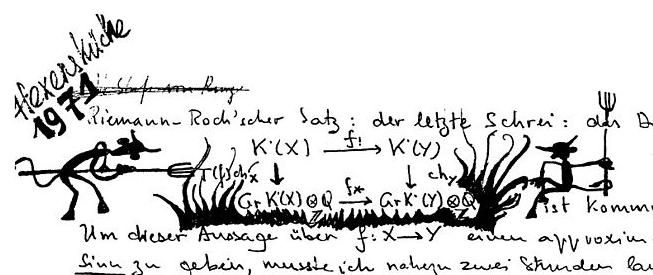
\includegraphics[scale=0.5]{grr.jpeg}
	\end{center}
	\caption{A famous drawing of the Grothendieck-Hirzebruch-Riemann-Roch formula from one of Grothendieck's notebooks. }\label{fig:grr}
\end{figure}

Here is the statement of the Theorem. 
We will explain what everything means after. 
\begin{theorem}
	Let $f:X\to Y$ be a proper morphism of schemes. 
	Let $E$ be a vector bundle on $X$. 
	The following identity holds in $A^{\bullet}(Y)$,
	\begin{equation}
	\ch(f_{!}E) \td(Y) = f_* (\ch(E)) \td(X).
	\end{equation}
	Another way of writing this is as a commutative diagram
	$$\begin{tikzcd}
	K_0(X) \ar[r,"f_!"] \ar[d, "\ch(\cdot)\td(X)"]& K_0(Y) \ar[d,"\ch(\cdot)\td(Y)"]\\
	A(X) \ar[r,"f_*"] & A(Y)
	\end{tikzcd}.$$
\end{theorem}
\begin{proof}[Proof Reference]
	\url{http://www.math.stonybrook.edu/~fgreer/IntersectionTheoryNotes.pdf}
\end{proof}

Given a coherent sheaf $E$ we define 
$$ f_!E = \sum_{i=0}^n (-1)^iR^if_*E $$
and this gives a map $f_!:K_0(X) \to K_0(Y)$.
The vertical maps say to take the \emph{chern character} $\ch(E)$ of your vector bundle and multiply it times the \emph{todd class}. 
To explain these I need to get into a bit more detail about the chern classes and the splitting principal since the definition of these two characteristic classes use the chern roots. 
Basically, the splitting principal is going to tell use that we can always treat vector bundles as if they were direct sums of line bundles. 
Then for line bundles, the chern character will just be the exponential function and the todd character will be the generating function for the Bernoulli numbers. 
The todd character of a scheme then is defined to the todd character of the tangent bundle on that scheme.

\subsection{The Grothendieck Group of Vector Bundles}
Everyone when they are first introduced to modules over commuative rings one notices the nice ring structure that they have: 
Given two modules $E$ and $F$ we can construct the modules $E \oplus F $ and $E \otimes F$.
These operations have the nice property that $E \otimes( F \oplus F') \cong E \otimes F \oplus E \otimes F'$.
To make this "ring" make sense as an actual ring we mod out by the relation of isomorphism. 
This gives
$$[E \oplus F ] = [E] + [F] \mbox{ and } [E \otimes F] = [E] \cdot [F] $$
There is actually a slighly better way of doing this and that is to using the relation
$$0 \to V \to E \to H \to 0 \implies [E] = [V] + [H] $$
In the free group of modules. 
We also have $[E\otimes F] = [E][F]$.

What Grothendieck did is only slighly fancier:
\begin{eqnarray*}
	K_0(X) &=& \mbox{(Grothendieck Group of Coherent Sheaves on $X$)}\\
	&=& \frac{\mbox{(Free Group of Coherent Sheaves on $X$)} }{\mbox{relations}}
\end{eqnarray*}
where we have the same relation among exact sequences. 
Since every vector bundle gives a coherent sheave by taking its sections we will consider this slightly more general setting.
Just as a remark, it turns out that the Grothendieck group of vector bundles and the Grothendieck group of coherent sheaves are actually the same most of the time so we are going to sweep this under the rug.

\iffalse 
\begin{remark}
	The reason we take coherent sheaves rather than just sheaves of $\Ocal_X$-modules is to make the category behave better with respect to morphisms.
	GIven a map $f: X \to Y$ there is a functor $f^*:\Coh_Y \to \Coh_X$ from the category of coherent modules on $Y$ to the category of coherent modules on $X$ given by
	$E \mapsto f^*E$. 
	Since $K_0(X) = \Coh_X/\sim$ as sets the functor $f^*$ then induces a functor on $K_0(X)$.
	This makes $K_0$ a functor to abelian groups.
\end{remark}
\fi 


\iffalse 
\begin{exercise}
	A $\lambda$-\emph{ring} is a ring $R$ equipped with a maps of sets $\lambda^i: R\to R$ for $i\in \NN$ satisfying the following properties
	\begin{enumerate}
		\item $\lambda^i \circ \lambda^j(a) = \lambda^{i+j}(a)$
		\item $\lambda^i( a \cdot b) = P_i(\lambda^1(a),\lambda^2(a),\ldots, \lambda^i(a),\lambda^1(b),\lambda^2(b),\ldots,\lambda^{i-1}(a))$
		\item $\lambda^i(a + b) = \sum_{j+k=i} \lambda^j(a) \lambda^k(b) $
	\end{enumerate}
	
	Show that $K_0(X)$ can be given the structure of a $\lambda$-ring 
	via $ \lambda^i: [E] \mapsto [\wedge^i E]. $
\end{exercise}
\fi



\subsection{Chern Classes}
Given a vector bundle $E$ of rank $r$ on a scheme $X$ we are going to define the chern classes $c_i(E)\in A^i(X)$ for $0\leq i \leq r$.
The key things we want are that $c_1(\Ocal_X(D)) = D \in A^1(X)$ for any Cartier divisor $D$ and that the class behave well with respect exact sequences. 
To explain what we mean by ``behave well'' let's first define the total chern class:
\begin{definition}
	Let $E$ be a vector bundle of rank $r$ on $X$.
	We define the \emph{total chern class} of $X$ to be the element of $A^{\bullet}(X) = \bigoplus_{i=0}^n A^i(X)$ given by 
	$$ c(E) = 1 + c_1(E)t + c_2(E)t^2 + \cdots + c_r(E)t^r. $$
	Here we are only using the variables $t$'s as decorations so that we know that these elements are in different degrees. 
\end{definition}
Now we can describe what we mean by behave well: we want $c:K_0(X)\to A^{\bullet}(X)$ to be a ring homomorphism. 
This means for any exact sequence 
$$ 0 \to V \to E \to H \to 0 \quad \implies \quad c(E) = c(H)c(V). $$
\iffalse 
Note that as $\Ocal_X(D)\otimes \Ocal_X(E) = \Ocal_X(D+E)$.
This suggests the rule $c(E\otimes F) = c(E)+c(F)$ which we will also impose.
\fi

\subsubsection{Splitting Principle}
If $E = \bigoplus_{i=1}^r L_i$ where $L_i$ are line bundles then we get to write 
$$ c(E) = \prod_{i=1}^r(1+c_1(L_i)t).$$
This implies that $c_i(E) = \sigma^{r}_i( c_1(L_1), c_1(L_2),\ldots, c_1(L_r) )$ where $\sigma^r_i$ is the $r$th symmetric polynomial in $i$ variables.
This symmetric polynomial has ${r \choose i}$ terms where the terms come from choosing $i$ of the variables and take their products.

For the purposes of computations we get to pretend that every vector bundle is the direct sum of line bundles.
This is because any symmetric polynomial can be written in a basis of symmetric polynomials. 
Generally we write
$$c(E) = \prod_{i=1}^r ( 1+ \alpha_i t )$$
and call $\alpha_i \in A^1(X)$ the \emph{chern roots} of $E$.
The fact that computations work out is called the \emph{splitting principle}. 

\begin{example}
	Let $E$ be a vector bundle of rank two. Using the splitting principle, we can compute $\Sym^2(E)$.
	We will suppose that $E = L\oplus M$ and then we have $c_t(E) = (1+\alpha t)(1+\beta t)$ where $\alpha=c_1(L)$ and $\beta=c_1(M)$. 
	This implies that $c_1(E) = \alpha+\beta$ and $c_2(E) =\alpha\beta$. 
	In the case that $E=L\oplus M$ we have $\Sym^2(E) = L^{\otimes 2}\oplus (L\otimes M) \oplus M^{\otimes 2}$ which means $c(\Sym^2(E)) = (1+2\alpha t)(1+(\alpha+\beta) t)(1+2\beta t)$ if you work this all out you get 
	$$ c_1(\Sym^2(E)) = 3c_1(E), \quad c_2 (\Sym^2(E)) = 2c_1(E)^2+2c_2(E), \quad c_3(\Sym^2(E)) = 4c_1(E)c_2(E).$$
	Here you need to use the identities for $c_1$ and $c_2$ in terms of $\alpha$ and $\beta$.
\end{example}

\begin{exercise}
	Compute $c(\Sym^n(E))$ and $c(\wedge^nE)$ for the first several $n$. 
	You may want to use the $\lambda$-ring structure for the wedge powers.
\end{exercise}



The following is an important fact that we will not prove. 
\begin{theorem}
	\begin{enumerate}
	\item If $X$ is a smooth complex projective variety of dimension $n$ and $T_X$ is its tangent bundle then $\deg(c_n(T_X)) = \chi_{\top}(X)$, the topological Euler characteristic. 
	\item $c_1(E) = c_1(\det(E))$; in particular $c_1(\Omega_X) = c_1(\omega_X)=K_X$ for $X$ regular.
	\item $c_i(E^{\vee}) = (-1)^i c_i(E)$. 
	\end{enumerate}
	%For any vector bundle $E$, and general $X$, $\deg(c_n(E))$ also counts the zeros of a general section of $s \in H^0(X,E)$ with multiplicity.
\end{theorem}


\subsection{Chern Characters}
We now come to Chern characters which also appear in the statement of Riemann-Roch.
\begin{definition}
	The \emph{Chern character} of $E$ is defined by the formula $\ch(E) = \sum_{i=1}^r e^{\alpha_i t}$
	where $\alpha_1,\ldots, \alpha_r$ are the Chern roots of $E$.
\end{definition}
One can break down the above definition to get 
\begin{align*}
\ch(E) =&\sum_{i=1}^r e^{\alpha_i}=\sum_{i=1}^r \left ( \sum_{j\geq 0}  \frac{\alpha_i^j}{j!}t^j \right) = \sum_{j\geq 0}  \sum_{i=1}^r \frac{\alpha_1^j + \alpha_2^j + \cdots + \alpha_r^j }{j!}t^j\\
=& \rk(E) + c_1t + \frac{c_1^2 - c_2 }{2}t^2 + \frac{c_1^2 - 3 c_1 c_2 + 2c_3}{6}t^3 \\
& + \frac{c_1^4 - 4c_1^2c_2 + 3 c_1c_3 + 2 c_2^2 + c_1c_2 - 4c_4}{24} t^4 + \cdots + n_r t^r
\end{align*}
Where $n_r$ is the last entry. 
Here we have written $c_i$ for $c_i(E)$. 
Also, on the last line uses the Newton identities which allows use to express the symmetric functions 
$$n_d(x_1,\ldots,x_r) = x_1^d+x_2^d+\cdots + x_r^d $$
in terms of elementary symmetric functions.
This is a symmetric polynomials and by the fundamental theorem of symmetric polynomials we have $n_s \in \ZZ[\sigma^r_1,\sigma^r_2,\ldots,\sigma^r_r]$.
The formulas for these are given by Newton's identities. 
The first several formulas are as follows:
\begin{align*}
n_0 &= r, \\
n_1 &= \sigma_1, \\
n_2 &= \sigma_2 - 2 \sigma_1,\\
n_3 &= \sigma_1^3 - 3 \sigma_1 \sigma_2 - 3 \sigma_3,\\
n_4 &= \sigma_1^4 - 4 \sigma_1^2 \sigma_2 + 4 \sigma_1 \sigma_3 + 2 \sigma_2^2 + 4\sigma_1 \sigma_2 - 4 \sigma_4.
\end{align*}
This will be sufficient for our purposes.
There is a recurrence that you can look-up on wikipedia if you ever need to go beyond this. 
\begin{exercise}
	Show that the chern character defines a ring homomorphisms $\ch: K^0(X) \to A^{\bullet}(X).$ One needs to show that $ 0 \to V \to E \to H \to 0$ implies $\ch(E) = \ch(V) + \ch(H)$ and that $ \ch(E \otimes F) = \ch(E)\ch(F)$.
\end{exercise}

\subsection{Todd Classes}
Recall that the Bernoulli Number are defined by the exponential generating function 
$$\frac{x}{e^x-1} = \sum_{j\geq 0} B_j \frac{x^j}{j!}.$$
As stated in the introduction, we use these to define the Todd class. 
\begin{definition}
	Let $E$ be a vector bundle on $X$ with chern roots $\alpha_1,\alpha_2,\ldots,\alpha_r$.
	The \emph{Todd character} of $E$ is defined by $\td(E) = \prod_{i=1}^r \frac{\alpha_i t}{1 - e^{-\alpha_i t}}$.
\end{definition}
Again, one does some computations and finds that 
\begin{align*}
\td(E) =& \prod_{i=1}^r \frac{\alpha_i t}{1 - e^{-\alpha_it}} = \prod_{i=1}^r \left( \sum_{j\geq 0} (-1)^j B_j  \alpha_i^j \frac{t^j}{j!}\right) \\
=& 1 + \frac{c_1}{2}t + \frac{c_1^2 +c_2}{12}t^2 + \frac{c_1c_2}{24}t^3 + \frac{-c_1^4 + 4 c_1^2 c_2 + c_1c_3 + 3c_2^2 - c_4}{720}t^4 + \cdots 
\end{align*}
In the above formula $c_i$ denotes $c_i(E)$. 
\begin{definition}
	For a scheme $X$ we define the \emph{todd class of $X$} to be $\td(X):= \td(T_X)$.
\end{definition}
As a warning, you will often see people write $c_i(X)$ for $c_i(T_X)$. 
A $c_i$ alone without specifying where it comes from can sometimes be ambiguous. 
You should worry about this a little when you first start working with these.

\begin{exercise}
	Show that if we have an exact sequence $0\to V \to E \to H \to 0$ we get $\td(E) = \td(V)\td(H)$.
\end{exercise}

Finally, Euler characteristics come into play because of how they are related to chern and todd classes. \taylor{I need to get my hands dirty again and check some of these}
\begin{theorem}
	Suppose that $\pi:X\to \Spec(K)$ is proper. 
	Then $ \chi(E) = \deg(\ch(E)\td(E)).$
\end{theorem}

\subsection{Examples}

\begin{example}
	When $X/K$ is a curve and $E$ is a vector bundle on $X$ we have 
	$\chi(E) = \deg(c_1(E)) + \rk(E)(1-g)$
	Note that when $E=L$ a line bundle of degree $d$ we have $\chi(L) = d-g+1.$
\end{example}

\begin{example}
	Here is the example for surfaces:
	\begin{center}
		\url{https://www.youtube.com/watch?v=3N3dvfHkG1o}.
	\end{center}
	
	
\end{example}

\begin{exercise}
	Prove Noether's Formula by Specializing the previous exercise to the trivial vector bundle:
	$$ \chi(\Ocal_S) = \frac{c_1(T_S)^2+c_2(T_S)}{12} = \frac{K_X^2+\chi_{\top}(S)}{12} $$
\end{exercise}

\begin{exercise}
	\begin{enumerate}
		\item Derive the Riemann-Roch formula for threefolds over a field. 
		\item Derive the Riemann-Roch formula for fourfolds over a field.
	\end{enumerate}
\end{exercise}

\section{27 Lines via Schubert Calculus}

This approach is nice because in addition to telling you that a cubic surface in $\PP^3$ has 27 lines it will also tell you things like quintic hypersurfaces in $\PP^4$ have 2875 lines. 

The long and the short of it is this: 
\begin{itemize}
	\item There exists a vector bundle of rank two $E$ on $\GG(1,3)$ such that a global section of $\Sym^3(E)$ corresponds to restricting a cubic form to various lines.
	This means vanishing locus of the section corresponds to the lines on this cubic form. 
	\item As it turns out the top chern class $c_4(\Sym^3(E)) \in A^4(\GG(1,3))=A_0(\GG(1,3))$ is the cycle of points which counts exactly this. 
	This is sometimes called the Euler class. 
	\item It also turns out that $A^{\bullet}(\GG(1,3))$ can be computed explicitly and furthermore that we are about to write out the chern classes of $E$ in this basis. This is Schubert calculus. 
\end{itemize}
From this we will compute 
$$ \deg( c_4(\Sym^3(E)) ) = 27 $$
which will give our result.

\subsection{Computation of $c_4(\Sym^3(E))$}
Let $X$ be any scheme. 
Let $E$ be a rank two vector bundle on $E$ and for simplicity we will write 
 $$a=c_1(E), \quad b = c_2(E). $$
These live in $A^1(X)$ and $A^2(X)$ respectively and with them we can write out the Chern polynomial:
 $$ c(E) = 1+at+bt^2.$$
Using the splitting principle we pretend $E = L \oplus M$ and write 
 $$ c(E) = (1+\alpha t) (1+\beta t)= 1+(\alpha+\beta)t + \alpha \beta t^2$$
where $\alpha$ and $\beta$ are the first chern classes of the fictitous line bundles $L$ and $M$. 
This gives 
 $$ a = \alpha + \beta, \quad b = \alpha \beta.$$
Now since 
$$\Sym^3(L\oplus M) = L^{\otimes 3} \oplus (L^{\otimes 2} \otimes M) \oplus (L\otimes M^{\otimes 2}) \oplus M^{\otimes 3},$$ 
we have that 
 $$ c(\Sym^3(E)) =(1+3\alpha t) (1+(2\alpha+\beta)t) (1+(\alpha+2\beta t))(1+3\beta t).$$
We can expand this our and get the various chern classes for $\Sym^3(E)$. 
We have, for example, 
 $$ c_1(\Sym^3 E) = 6(\alpha+\beta), \quad c_4(\Sym^3 E) = 9 \alpha \beta ( 5\alpha\beta + 2(\alpha^2+\beta^2)). $$
We now just need to write these in terms of elementary symmetric polynomials $a,b$.
The first one is obvious: $c_1(\Sym^3(E)) = 6a=6c_1(E)$.
Being clever and writing 
$$\alpha^2+\beta^2 = (\alpha+\beta)^2-2\alpha\beta=a^2-2b$$ 
gives us a formula for the second one:
 $$ c_4(\Sym^3(E)) = 9 b ( 5b + 2(a^2-2b))=18ba^2+9b^2.$$
In the case of our particular application it will turn out that $ba^2 = b^2$ and both have degree one which will imply that 
$$ \deg(c_4(\Sym^3(E))) = 18+9 =27,$$
hence the 27 lines on a cubic surface. 

\subsection{Schubert Cycles}
\taylor{I need to add more here}
\newpage
 
\appendix


 


%%%%%%%%%%%%%%%%%%%%%%%%%%%%%%%%%%%%%%%%%
%%%%%%%%%%%%%%%%%%%%%%%%%%%%%%%%%%%%%%%%%

\section{Nakayama's Lemma: Stalk Local to Affine Local}
The version of Nakayama that you hear in a commutative algebra class is this: if $R$ is a local noetherian ring with maximal ideal $M$ and $V$ is a finitely presented $R$-module (or just finitely generated because we are working over a Noetherian ring) then 
$$ MV =V \implies V =0. $$
The proof relies on the Cayley-Hamilton theorem and relies on producing an element (which ends up being a determinant) which is a unit and which annihilates $V$. 
There is another version where $V$ is finitely generated and we only need to assume that $IV=V$ where $I$ is contained in the jacobson radical (the intersection of all maximal ideals)--- the proof is exactly the same. 

For the untrained eye, these theorems look useless, but these theorems are really about extending stalk-local information of coherent sheaves (the analog of finitely presented) to affine-local information. 

The first version says that if you are zero at a point then you are zero in a neighborhood:
\begin{theorem}[Nakayama: vanishing version]\label{thm:nakayama-vanishing}
	Let $X$ be a Noetherian scheme and let $F$ be a coherent $\Ocal_X$-module. 
	Let $x\in X$. 
	$$F_x \otimes_{\Ocal_{X,x}}\kappa(x) =0 \implies F\vert_U =0. $$
	By the statement on the right we mean that there exists an open $U$ containing $x$ such that this holds.
\end{theorem}

\begin{theorem}[Nakayama: generators version]
	Let $X$ be a Noetherian scheme and let $F$ be a coherent $\Ocal_X$-module. 
	Let $U\subset X$ be an open subscheme containing $x$.
	If $s_1,\ldots,s_n \in F(U)$ have the property that $\overline{s}_1,\ldots,\overline{s}_n\in F_x\otimes_{\Ocal_{X,x}} \kappa(x)$ generate $F_x$ then there exists some $U_0 \subset U$ containing $x$ such that $s_1,\ldots,s_n$ generate $F\vert_{U_0}$.
\end{theorem}

\begin{theorem}[Nakayama: rank version]\label{thm:nakayama-rank}
	Let $X$ be a Noetherian scheme and $F$ a coherent $\Ocal_X$-module.
	Define 
	$$ e(x) := \dim_{\kappa(x)}\left( F_x \otimes_{\Ocal_{X,x}} \kappa(x) \right). $$
	\begin{enumerate}
		\item 	The function $e(x)$ is upper semicontinuous. 
		This means that the sets $ \lbrace x \in X \colon e(x)\leq r \rbrace$
		are open for all $r\in \RR$.
		\item Assume $X$ is reduced. 
		Let $x\in X$. 
		There exists some $U\owns x$ open such that $F\vert_U$ is free if and only if there exists some $V \owns x$ open such that $e$ is constant on $V$.
	\end{enumerate}
\end{theorem}
I learned this all from Mumford's Red Book, Atiyah-MacDonald, and Eisenbud's Commutative Algebra.


\section{Flatness}
Here we give a good practical discussion of how to determine if a scheme is flat. 
My favorite place to read about flatness is Mumford's Red Book.

One should recall that an $R$-module $V$ is flat if and only if the functor $\otimes_RV$ from $R$-modules to $R$-modules is left exact. 
We should now that right exactness comes for free since cokernels are colimits, $-\otimes_R V$ is a left adjoint of $\Hom_R(V,-)$, and left adjoints preserve limits. 
There are a couple other tests that are useful. 
For example it suffices to test $I\otimes_R V \to IV$ is injective for every ideal $I$ to show that $V$ is a flat $R$-module. 

Another important property is that flatness is stalk-local.
We have thet $V$ is a flat $R$-module if and only if for every prime ideal $P$ we have $V_P$ is a flat $R_P$-module. 
We actually have something even stronger: one only needs to check this for $P$ a maximal ideal.
Furthermore, over a local noetherian ring flat, projective, and free are all the same thing.
So flat is another way of saying locally free (one thing to keep in mind is that it won't necessarily be locally free of finite rank... for example $R[x]$ is a flat $R$-module). 

This stalk-locality property allows us to transfer this notion to schemes. 
We say that a sheaf of modules $\Fcal$ on $X$ is flat if it is $\Fcal_x$ is a flat $\Ocal_{X,x}$-module for every $x\in X$ (or every closed point). 
We say a morphism of schemes $X \to S$ is flat if and only if $\Ocal_{X,x}$ is a flat $\Ocal_{S,s}$-module. 



\subsection{Flatness over a DVR}
Let $R$ be a DVR with uniformizer $t$.
An $R$-module $M$ is flat if and only if multiplication by $t$ is injective on $M$. 
This is a very useful way to check to see if things are flat.

\begin{example}
	The map $k[x,y]/(xy)$ is not a flat $k[x]$-module. 
	We have $k[x]_{(x)} \to (k[x,y]/(xy))_{(x,y)}$ and after taking completions we have $k[[x]] \to k[[x,y]]/(xy)$ and we see that multiplication by $x$ in $k[[x,y]]/(xy)$ is not injective.\footnote{Flatness can be deduced from flatness at the completion because the maps $A \to \widehat{A}$ are faithfully flat.}
\end{example}

\begin{example}
	The map $k[x] \to k[x,y]/(y^2,xy)$ is not flat. 
	Again we see that $k[x]_{(x)} \to (k[x,y]/(y^2,xy))_{(x,y)}$ is not flat since multiplications by $x$ is not injective. 
\end{example}


\subsection{Flat limits}
Here we follow McKernan's Lecture notes:
\begin{center}
	\url{https://math.mit.edu/~mckernan/Teaching/07-08/Spring/18.726/l_14.pdf}
\end{center}
What we are going to be doing here is talking about taking limits of families. 
As usual ``families'' are fibers of a morphism. .

\begin{itemize}
	\item Let $S$ be a one dimensional regular scheme.
	\item Let $X$ be a closed subscheme of $W\times S$. 
	\item Let $\pi:X\to S$ be a morphism of schemes.
	\item Let $s\in S$ be a closed point. 
	\item Let $S^* = S \setminus  s$
	\item Let $X^* = \pi^{-1}(S^*)$.
	\item Let $X_s=\pi^{-1}(s)$ be the fiber above $s\in S$. 
\end{itemize}
We say that $X_s$ is a \emph{flat limit} of $X^*$ at $s$ if the scheme theoretic closure of $X^*$ is $X$. 

\begin{remark}
	Later we will show that $\Ocal_{X,s}$ is a flat $\Ocal_{S,s}$-module in this situation.
\end{remark}

We recall briefly the definition of scheme theoretic closure.
Since $i:X^* \subset W\times S$ we have $\Ocal_{W\times S} \to i_*\Ocal_{X^*}$.
The kernel of this morphism is an ideal sheaf $I$ which cuts our the scheme theoretic closure in $W\times S$. 



In what follows we remind the reader that $\Irr(X)$ denotes the irreducible components of $X$.
\begin{lemma}
	Let $X$ be a scheme. 
	Let $Z\subset X$ is a closed subscheme. 
	$$ \Irr(X) = \Irr_Z(X) \amalg \Irr(X\setminus Z)$$
	and $\Irr_Z(X)$ are the irreducible components of $X$ lying in $Z$.
\end{lemma}
\begin{proof}
	If $Y$ is an irreducible component of $X$ and $X = X' \cup X''$ with $X'$ and $X''$ then $Y \subset X'$ or $Y \subset X''$. 
	If not then $Y = (Y \cap X') \cup (Y \cap X'')$ is a decomposition into irreducible components. 
	We have $X = \overline{U} \cup Z$ and hence, by what was said previously every irreducible component is either in $\overline{U}$ or $Z$. 
\end{proof}

Next we give a criteria for $X_s$ being a flat limit. 

\begin{theorem}
	The scheme $X_s$ is the flat limit of $X^*$ at $s$ if and only if $X_s$ contains no components of $X$ (see figure~\ref{fig:flat-limit} for a picture of a non-flat limit).
\end{theorem}

	\begin{figure}[h]
	\begin{center}
		\includegraphics[scale=0.4]{flat-limit.eps}
	\end{center}
	\caption{A picture of a non-flat limit. You can see the fiber has irreducible components.}\label{fig:flat-limit}
\end{figure}


\begin{proof}
	Let $s=0$ for simplicity.
	We always have $\Irr(X) = \Irr(X^*) \amalg \Irr(X_0)$.
	We have $\Irr(\overline{X^*}) = \Irr(X^*)$ and hence if $\overline{X^*}=X$ then $\Irr_{X_0}(X)=\emptyset.$.  
	This proves that when we have a flat limit, the fiber contains no components. 
	
	Conversely, suppose that the fiber contains no components. 
	Then by the irreducible component equation, all the irreducible components must be in $\overline{X^*}$ which shows $\overline{X^*}=X$.
\end{proof}


\begin{theorem}
	$X_s$ is the flat limit of $X^*$ at $s$ if and only if for every closed point $x \in X$ with $\pi(x)=s$ the localization $\Ocal_{X,x}$ is a flat $\Ocal_{S,s}$-module. (In the case when $S$ is regular of dimension one, and $t$ is a uniformizer at $s$, this is equivalent to $\Ocal_{X,x}$ being $t$-torsion free).
\end{theorem}
\begin{proof}
Without loss of generality we can assume that $S = \Spec(R)$. 
\begin{itemize}
	\item We first show that not flat implies not a flat limit:
		We will let $s=0$ for simplicity and let $t$ be a uniformizer at $0$. 
	Suppose that $\pi(x)=0$ and $R_{(t)} = \Ocal_{S,0} \to \Ocal_{X,x}$ is not flat. 
	Then there is some $f$ such that $tf=0$. 
	This can be lifted to an affine open since localizations are a direct limit of principal localizations. 
	This means that $f$ vanishes identically on some irreducible component of $X$ (also $t$ vanishes identically on some irreducible component); this component is contained in $X_0$. 
	
	By the previous theorem, $X_0$ is a flat limit if and only if it doesn't contain any components of $X$, which tells us that $X_0$ is not flat.  
	
	\item We now show that not a flat limit implies not flat. 
	Suppose  that $Z \subset X_0$ is a schematic component of $X$. 
	We need to show there is a closed point $x \in X_0$ such that $R_{(t)} =\Ocal_{S,0} \to \Ocal_{X,x}$ which is not flat. 
	Let $\Spec(A)\subset X$ be an affine open containing $x$ so that $\Ocal_{X,x} = A_{m_x}$ where $m_x$ is the maximal ideal of $x$ in $A$.
	This means we need to find some $f \in \Ocal_{X,x}$ which is annhilated by $t$.
	Note that $tA \subset m_x$ so $t$ is not a valid denominator in $A_{m_x}$.
	
	Let $I_Y$ be the ideal cutting out $Y$, the union of all components not contained in $X_0$. See Figure~\ref{fig:flat-limit} for a picture.
	Note that $f \in I_Y$ means that $f \vert_Y=0$ and in particular $f\vert_{X^*}=0$.
	See Figure~\ref{fig:flat-limit} for a picture. 
	Also, since $X^*$ is the localization at $t$, this means that $f\vert_{X^*}=0$ if and only if $t^nf =0$ for some $f$. 
	
	Now, the condition of minimality of primary decompositions says that we can pick any component and find a function which vanishes on all the other components except the one we chose. 
	In particular because it is a non-zero element and it is not a unit, there is a maximal ideal which contains $f$ which means that the localization of $f$ at $m_x$ is non-zero.
	Note that this maximal ideal can be viewed both as a maximal ideal of $\Ocal(X_0)$ and $\Ocal(X)$.
	This gives an element of $\Ocal_{X,x}$ which is annihilated by $t$ and hence $\Ocal_{S,s} \to \Ocal_{X,x}$ is not flat.
\end{itemize}

\begin{example}
	A consequence of this is that the blow-up at a point is not flat. 
\end{example}

\end{proof}

\section{Supports}

\taylor{I need to check this section. I'm a little worried about the schematic version.}
Let $F$ be a sheaf of modules on a scheme $X$. 
We will first define the support of a sheaf of modules as a subset of the underlying topological space. 
Later, we will give it a scheme structure. 
\begin{definition}[Preliminary Definition]
	The collection of points $x\in X$ such that $F_x\neq 0$ is called the \emph{support of $F$}. We denote this set as $\supp(F)$.
\end{definition}

There is a version of Nakayama's Theorem (Theorem~\label{thm:nakayama-vanishing}) that tells us the place where $F_x=0$ is is an open subset of the topological space. 
This means the collection where $F_x\neq 0$ is closed (this is sort of the opposite of the way that we are used to think of functions where vanishing is a closed condition).
We want more than just this. 
We would like $\supp(F)$ to be a closed subscheme. 
In terms of modules have scheme structures, the main thing that we want is that $\widetilde{R/I}$ as an $\Ocal_{\Spec R}$-module have support $\Spec(R/I)$ on $\Spec(R)$.

\subsection{Supports of Modules}

\begin{lemma}
	Let $I\subset A$ be an ideal. 
	We have $\supp(A/I) = V(I)$ as subsets of $\Spec(A)$.
\end{lemma}
\begin{proof}
	Let $P\in V(I)$. This means $P\supset I$. 
	Let $l_P: A/I \to (A/I)_P$ be the localizations map.
	It has a kernel consisting of all the elements which are annihilated by $S = A\setminus P$. 
	Since $P \supset I$ we have $A\setminus P \subset A\setminus I$ and no elements are killed. 
	This means $P\in \supp(A/I).$
	
	Conversely, let $P \in \supp(A/I)$. 
	Then $l_P: A/I \to (A/I)_P$ is nonzero. 
	This means that $S=A\setminus P$ does not annihilate 1 which means $(A\setminus P)\cap I = \emptyset$ whcih means $P \supset I$ or that $P \in V(I)$.
\end{proof}

\begin{lemma}
	Let $M$ be an $A$-module. We have $\supp(M) = V(A/\ann_A(M))$.
\end{lemma}
\begin{proof}
	We show that $\supp(M)=\supp(A/\ann(M))$. 
	By the previous lemma this will give the result. 
	For simplicity of notation we let $I = \ann(M)$. 
	
	If $P\in \supp(M)$ then $M_P$ is nontrivial $(A/I)_P$-module which means $(A/I)_P$ is nontrivial and $P\in \supp(A/I)$. 
	
	Conversely, let $P\in \supp(M)$. 
	Since $M$ is nontrivial, there is always a cyclic $(A/I)$-module in $M$, otherwise we could increase the annihilator. 
	Let the generator of the cyclic submodule be $x$. 
	We have 
	\begin{align*}
	(A/I)_P \neq 0 &\implies ((A/I) \cdot x)_P \neq 0 \\
	&\implies M_P \neq 0. 
	\end{align*}
	This proves $\supp(A/I)\subset \supp(M)$. 
\end{proof}

\subsection{Scheme structure}
Let $F$ be a sheaf of $\Ocal_X$-module. 
We define $\ann_X(F)$ to be the sheaf associated to the presheaf 
$$ U\mapsto \ann_{\Ocal_X(U)}(F(U)).$$
We then define $\supp(F)$ to be the subscheme associated to $\ann_X(F)$.





\end{document}
